% ===================================================================
%  EN48  Cannizzo《亏格 2 曲线的同调镜像对称》中文译注本  汇总文件
% ===================================================================
% ===================================================================
%  EN48  Cannizzo《亏格 2 曲线的同调镜像对称》中文译注本  导言区
%  本工程由译者（翻译智能体）全权维护；改动须记入 README 变更日志
% ===================================================================
\documentclass[11pt,a4paper]{article}

\usepackage[UTF8]{ctex}
\usepackage{amsmath,amssymb,amsthm,mathtools}
\usepackage{mathrsfs}
\usepackage{bm}
\usepackage{graphicx}
\usepackage{tikz}
\usepackage{tikz-cd}
\usepackage[a4paper,top=2.4cm,bottom=2.6cm,left=2.4cm,right=2.4cm]{geometry}
\usepackage[dvipsnames]{xcolor}
\usepackage{enumitem}
\usepackage{array}
\usepackage{multicol}
\usepackage{fancyhdr}
\usepackage{caption}
\usepackage{titlesec}
\usepackage[hidelinks,bookmarksnumbered]{hyperref}

% ---------- 版面 ----------
\linespread{1.18}
\setlength{\parindent}{2em}
\setlength{\parskip}{0.25em}
\captionsetup{font=small}

% ---------- 页眉页脚 ----------
\pagestyle{fancy}
\fancyhf{}
\fancyhead[L]{\small 亏格 2 曲线的同调镜像对称}
\fancyhead[R]{\small 中文译注本}
\fancyfoot[C]{\small\thepage}
\renewcommand{\headrulewidth}{0.3pt}

% ---------- 章 / 节标题（原文为 Chapter N，故 section 显示为「第 N 章」） ----------
\newcommand{\seclabel}{第 \thesection{} 章}
\titleformat{\section}{\Large\bfseries}{\seclabel}{1em}{}
\titleformat{\subsection}{\large\bfseries}{\thesubsection}{0.8em}{}
\titlespacing*{\section}{0pt}{2.2ex plus 1ex minus .2ex}{1.2ex plus .2ex}
\titlespacing*{\subsection}{0pt}{1.8ex plus 1ex minus .2ex}{0.8ex plus .2ex}

% ---------- 定理类环境 ----------
% 原文编号形如 1.2.3（章.节.该节内序号），且各种环境共用同一计数器（例：
% Remark 1.2.1 与 Definition 1.2.2 连续编号）。故全部环境挂到同一个 result 计数器，
% 该计数器随 subsection 归零。定理类一律不手工写编号，用 \label/\ref。
\theoremstyle{definition}
\newtheorem{result}{结果}[subsection]
\newtheorem{theorem}[result]{定理}
\newtheorem{proposition}[result]{命题}
\newtheorem{lemma}[result]{引理}
\newtheorem{corollary}[result]{推论}
\newtheorem{definition}[result]{定义}
\newtheorem{example}[result]{例}
\newtheorem{claim}[result]{断言}
\newtheorem{remark}[result]{注}
\newtheorem{conjecture}[result]{猜想}
\newtheorem{problem}[result]{问题}
\renewcommand{\proofname}{证明}
\renewcommand{\qedsymbol}{$\square$}
\renewcommand{\refname}{参考文献}

% 公式、图、表按章编号：(1.1)、图 1.1
\numberwithin{equation}{section}
\numberwithin{figure}{section}
\numberwithin{table}{section}

% ---------- 译者注 ----------
\newcommand{\transnote}[1]{%
  \par\medskip\noindent
  {\small\color{Sepia}\textbf{【译者注】}#1\par}\medskip}

% ---------- 常用记号 ----------
\newcommand{\R}{\mathbb{R}}
\newcommand{\C}{\mathbb{C}}
\newcommand{\Z}{\mathbb{Z}}
\newcommand{\Q}{\mathbb{Q}}
\newcommand{\N}{\mathbb{N}}
\newcommand{\PP}{\mathbb{P}}
\newcommand{\KK}{\mathbb{K}}
\newcommand{\OO}{\mathcal{O}}
\newcommand{\GG}{\mathcal{G}}
\newcommand{\HH}{\mathcal{H}}
\newcommand{\MM}{\mathcal{M}}
\newcommand{\LL}{\mathcal{L}}
\newcommand{\de}{\mathrm{d}}
\newcommand{\dd}{\mathrm{d}}
\newcommand{\id}{\mathrm{id}}
\newcommand{\pt}{\mathrm{pt}}
\newcommand{\rk}{\operatorname{rk}}
\newcommand{\tr}{\operatorname{tr}}
\newcommand{\sgn}{\operatorname{sgn}}
\newcommand{\vol}{\operatorname{vol}}
\newcommand{\supp}{\operatorname{supp}}%
\newcommand{\Coker}{\operatorname{Coker}}
\newcommand{\Ker}{\operatorname{Ker}}
\newcommand{\Hom}{\operatorname{Hom}}
\newcommand{\End}{\operatorname{End}}
\newcommand{\Aut}{\operatorname{Aut}}
\newcommand{\GL}{\operatorname{GL}}
\newcommand{\U}{\mathrm{U}}
\newcommand{\SU}{\mathrm{SU}}
\newcommand{\SO}{\mathrm{SO}}
\newcommand{\Sp}{\mathrm{Sp}}
\newcommand{\Spin}{\mathrm{Spin}}

% 花体字母
\newcommand{\cA}{\mathcal{A}}\newcommand{\cB}{\mathcal{B}}
\newcommand{\cC}{\mathcal{C}}\newcommand{\cD}{\mathcal{D}}
\newcommand{\cE}{\mathcal{E}}\newcommand{\cF}{\mathcal{F}}
\newcommand{\cG}{\mathcal{G}}\newcommand{\cH}{\mathcal{H}}
\newcommand{\cI}{\mathcal{I}}\newcommand{\cJ}{\mathcal{J}}
\newcommand{\cK}{\mathcal{K}}\newcommand{\cL}{\mathcal{L}}
\newcommand{\cM}{\mathcal{M}}\newcommand{\cN}{\mathcal{N}}
\newcommand{\cO}{\mathcal{O}}\newcommand{\cP}{\mathcal{P}}
\newcommand{\cQ}{\mathcal{Q}}\newcommand{\cR}{\mathcal{R}}
\newcommand{\cS}{\mathcal{S}}\newcommand{\cT}{\mathcal{T}}
\newcommand{\cU}{\mathcal{U}}\newcommand{\cV}{\mathcal{V}}
\newcommand{\cW}{\mathcal{W}}\newcommand{\cX}{\mathcal{X}}
\newcommand{\cY}{\mathcal{Y}}\newcommand{\cZ}{\mathcal{Z}}
% 哥特体字母
\newcommand{\fA}{\mathfrak{A}}\newcommand{\fB}{\mathfrak{B}}
\newcommand{\fC}{\mathfrak{C}}\newcommand{\fD}{\mathfrak{D}}
\newcommand{\fE}{\mathfrak{E}}\newcommand{\fF}{\mathfrak{F}}
\newcommand{\fG}{\mathfrak{G}}\newcommand{\fH}{\mathfrak{H}}
\newcommand{\fI}{\mathfrak{I}}\newcommand{\fJ}{\mathfrak{J}}
\newcommand{\fK}{\mathfrak{K}}\newcommand{\fL}{\mathfrak{L}}
\newcommand{\fM}{\mathfrak{M}}\newcommand{\fN}{\mathfrak{N}}
\newcommand{\fO}{\mathfrak{O}}\newcommand{\fP}{\mathfrak{P}}
\newcommand{\fQ}{\mathfrak{Q}}\newcommand{\fR}{\mathfrak{R}}
\newcommand{\fS}{\mathfrak{S}}\newcommand{\fT}{\mathfrak{T}}
\newcommand{\fU}{\mathfrak{U}}\newcommand{\fV}{\mathfrak{V}}
\newcommand{\fW}{\mathfrak{W}}\newcommand{\fX}{\mathfrak{X}}
\newcommand{\fY}{\mathfrak{Y}}\newcommand{\fZ}{\mathfrak{Z}}

% ---------- 杂项 ----------
\newcommand{\eps}{\varepsilon}
\newcommand{\iso}{\cong}
\newcommand{\into}{\hookrightarrow}
\newcommand{\onto}{\twoheadrightarrow}
\newcommand{\restr}[2]{{#1}\big|_{#2}}
\newcommand{\ip}[2]{\langle #1,#2\rangle}
\newcommand{\Vdual}{V^{\vee}}
\newcommand{\DBCoh}{\mathrm{D}^{\mathrm{b}}\mathrm{Coh}}
\allowdisplaybreaks[2]
\emergencystretch=2em


\begin{document}

\begin{center}
  {\LARGE\bfseries 亏格 2 曲线的同调镜像对称}\\[0.6em]
  {\large 及其广义 Strominger--Yau--Zaslow 镜像}\\[1.0em]
  {\large 中文译注本}\\[1.0em]
  {\large Catherine Kendall Asaro Cannizzo}\\[0.3em]
  {\small University of California, Berkeley, Department of Mathematics}\\[1.0em]
  {\small 底本：PhD dissertation, University of California, Berkeley, Spring 2019；\\
  eScholarship \texttt{qt88g945z7}；145 页}
\end{center}

\vspace{0.6em}
\noindent\rule{\textwidth}{0.4pt}
\begin{minipage}{\textwidth}
\small
\textbf{译本说明}\quad
底本为 Catherine Kendall Asaro Cannizzo 2019 年在加州大学伯克利分校提交的博士学位论文
\emph{Homological mirror symmetry for the genus 2 curve in an abelian variety and its
generalized Strominger--Yau--Zaslow mirror}（导师 Denis Auroux；答辩委员会 Nadler、Shapiro）。
原书 145 页；正文页码 1--136，前置页用罗马数字 i--v。原书 PDF 页与原书页码的换算是
\textbf{原书页 = PDF 页 $-9$}：PDF 第 10 页即原书第 1 页。源码中每页起首以注释行
\texttt{\% ===== 原书 p.N =====}（前置页为 \texttt{FRONT MATTER}）标出，便于对照原书。
原书全部内容（定义、定理、注、公式、图）均有编号，编号形式为「章.节.序号」，本译本
用 \LaTeX{} 自动编号，正文中以 \verb|\ref| 引用，不手工填写编号。译文中的
\textbf{【译者注】}为译者所加，只分三类：易错预警、含糊点拨、背景直觉，不代替读者
阅读原文，也不替作者补证明。人名与未定译名的术语保留英文原名，术语首次出现时括注英文。
\end{minipage}
\noindent\rule{\textwidth}{0.4pt}

\vspace{1.2em}
\noindent\textbf{内容提要}\quad
受物理学中的观察启发，镜像对称是说某些流形成对出现：$X$ 与 $Y$，且 $X$ 上的复几何
与 $Y$ 上的辛几何互为镜像，于是可以由 $X$ 的已知性质推断 $Y$ 的信息。
Strominger--Yau--Zaslow（1996）指出这类配对在几何上可由具有同一底空间、纤维相互
关联的环面丛给出，即 SYZ 镜像对称。Kontsevich（1994）进一步猜想：$X$ 上的一个复
不变量（有界相干层导出范畴）应当等价于 $Y$ 上的一个辛不变量（深谷范畴），此即同调
镜像对称。本文先用 Abouzaid--Auroux--Katzarkov 关于阿贝尔簇中超曲面的 SYZ 镜像构造
得到流形 $X$ 与 $Y$：复流形一侧取亏格 2 曲线作为其 Jacobi 环面中的超曲面，并给 SYZ
镜像流形配上一个辛形式；随后把复一侧的范畴嵌入 $Y$（视为辛纤维丛）的一个上同调
Fukaya--Seidel 范畴，证明该嵌入在上同调意义下全忠实。本文的纤维丛属于最早被赋予
深谷范畴的非正合、非 Lefschetz 纤维丛之列，但定义它的主要几何想法与 Seidel 对
Lefschetz 纤维丛的深谷范畴的构造相同。

\vspace{0.8em}
\noindent{\small 2010 年数学主题分类：主分类 53D37；次分类 14J33, 53D40}

\vspace{0.4em}
\noindent{\small 关键词：同调镜像对称，SYZ 镜像对称，深谷范畴，导出范畴，环簇}

\vspace{1.4em}
\tableofcontents
\newpage

% EN48 c00 | 原书 PDF 1–9（原书 i–v） | 前置页：摘要、献词、致谢（封面/版权页信息并入扉页，目录与图目录由 LaTeX 生成）
% 骨架文件：标题行已设定，正文由译者填写。每页起首用 % ===== FRONT MATTER (PDF n) ===== 注释标记。
% ===== FRONT MATTER (PDF 4) =====
\section*{摘要}
\addcontentsline{toc}{section}{摘要}

\begin{center}
{\small
亏格 2 曲线的同调镜像对称及其广义 Strominger--Yau--Zaslow 镜像\\[0.4em]
Catherine Kendall Asaro Cannizzo\\
数学哲学博士，University of California, Berkeley\\
导师：Denis Auroux 教授（主席）
}
\end{center}

受物理学中的观察启发，镜像对称是说某些流形成对出现：$X$ 与 $Y$，且 $X$ 上的复几何与
$Y$ 上的辛几何互为镜像，于是可以由 $X$ 的已知性质推断 $Y$ 的信息。
Strominger--Yau--Zaslow（1996）指出，这类配对在几何上来自具有同一底空间、纤维相互关联的
环面丛，称为 SYZ 镜像对称。Kontsevich（1994）猜想：$X$ 上的一个复不变量（有界相干层
导出范畴）应当等价于 $Y$ 上的一个辛不变量（深谷范畴）。此即同调镜像对称。本项目先用
Abouzaid--Auroux--Katzarkov 关于阿贝尔簇中超曲面的 SYZ 镜像构造，得到作为流形的 $X$
与 $Y$。复流形一侧来自亏格 2 曲线作为其 Jacobi 环面中的超曲面；我们给 SYZ 镜像流形
配上一个辛形式。随后描述复一侧的范畴到 $Y$（视为辛纤维丛）的一个上同调
Fukaya--Seidel 范畴的嵌入。本文的纤维丛属于最早配备深谷范畴的非正合、非 Lefschetz
纤维丛之列，但定义它的主要几何想法与 Seidel 对 Lefschetz 纤维丛的深谷范畴的构造相同。

\transnote{摘要里的 ``bounded derived category of coherent sheaves'' 即正文的
$\DBCoh$，本译本统一作「有界相干层导出范畴」。注意此处的 ``embedded'' 是范畴嵌入，
不是流形嵌入：$H$ 本身是 $V$ 中的超曲面，这里说的是 $\DBCoh(H)$ 嵌入 $Y$ 的
Fukaya--Seidel 范畴。}

\transnote{``cohomological Fukaya--Seidel category'' 指把态射复形取上同调后得到的
普通范畴，记作 $H^0(\mathrm{FS}(Y,v_0))$；它丢掉了 $A_\infty$ 的高阶运算，
所以第 4、5 章证明的只是上同调层面的等价，而非 $A_\infty$-等价。}

\transnote{``nonexact'' 指辛形式 $\omega$ 不正合：$Y$ 是带有紧纤维的辛纤维丛，
纤维体积非零，故 $\omega$ 不是恰当形式。这与 Seidel 在 [Sei08] 中处理的
Lefschetz 纤维丛（正合情形）有实质差别。}

\transnote{``Jacobian torus'' 即 $\mathrm{Pic}^0(\Sigma_2)$，见 \S 1.2：
固定点 $x_0$ 后，$x\mapsto\OO(x-x_0)$ 把 $\Sigma_2$ 嵌入这个二维阿贝尔簇。
「Jacobi 环面」与「阿贝尔簇」在本文指同一个对象的不同侧面，前者强调它是复环面。}

% ===== FRONT MATTER (PDF 5) =====
\section*{献词}
\addcontentsline{toc}{section}{献词}

\begin{center}
谨以本论文献给我的父亲 John Kendall Cannizzo，献上我全部的爱。

感谢您做我生命中的阳光。愿您安息。
\end{center}

\transnote{献词中的人名保留英文原名，不音译。这是全书的通例：凡作者、导师、
被致谢者，一律照录原文。}

% ===== FRONT MATTER (PDF 9) =====
\section*{致谢}
\addcontentsline{toc}{section}{致谢}

本工作部分受 NSF 基金 DMS-1264662、DMS-1406274、DMS-1702049 与 Simons Foundation
基金（\# 385573，Simons 同调镜像对称合作项目）资助。感谢我的导师 Denis Auroux
在本论文项目上无法估量的学术支持与指导。感谢 Mohammed Abouzaid、Melissa Liu、
Katrin Wehrheim、Sheel Ganatra、Heather Lee、Roberta Guadagni、Jingyu Zhao、
Sara Venkatesh、Wolfgang Schmaltz、Zhengyi Zhou、Benjamin Filippenko，以及 MSRI
导出范畴项目 [APS] 与我的有益数学讨论。感谢 Jo Nelson、Ailsa Keating、Bahar Acu、
Ziva Myer、Yu Pan、Morgan Weiler 与 Anastasia Chavez 在申请过程与职业发展上给予的
宝贵建议与支持。感谢 Noetherian Ring 与 UC Berkeley 数学系的工作人员。最后，
感谢我的父母始终不渝的支持。

\transnote{``Noetherian Ring'' 是 UC Berkeley 数学系的研究生学术组织，不是环论
概念。这里按专名保留英文，避免误读成「诺特环」。}

\transnote{MSRI 即 Mathematical Sciences Research Institute（伯克利）。
``Derived Categories program'' 指 2018 年前后 MSRI 的导出范畴专题项目，
方括号 [APS] 是原文的引用标记，指参与该项目的 Abramovich--Polishchuk--Segal
等人在相关主题上的工作；详见参考文献。}

\transnote{致谢中的基金编号照录原文。``Simons Collaboration on Homological
Mirror Symmetry'' 是 Simons Foundation 资助的协作项目，不是期刊或会议。}

% EN48 c01 | 原书 p.1–12 及 p.13 上半（§1.2 收尾）（PDF 10–22） | 第 1 章 §1.1–1.2
% 块骨架：标题行已设定，正文由译者填写。每页起首用 % ===== 原书 p.N ===== 注释标记。
% 边界说明：原书第十三页上半仍属 §1.2（三条结果收尾），
% 为保持小节与定理编号连续，归入本块；c02 从 §1.3 起。
\section{引言、背景与设定}

\subsection{论文结果与方法的陈述}

% ===== 原书 p.1 =====
本文中，代词「我们」兼指作者与读者。

\begin{theorem}\label{thm:main}
设 $\iota\colon H := \Sigma_2 \hookrightarrow V$ 为亏格 $2$ 曲线到复维数 $2$ 的阿贝尔簇
$V$ 的嵌入。则存在镜像 $(Y,v_0)$：它是辛纤维丛，纤维记作 $\Vdual$，与 $V$ 互为镜像；
$\Vdual$ 也是复维数 $2$ 的阿贝尔簇。于是有下面的交换图，图中竖直箭头是范畴之间的
上同调意义下全忠实嵌入函子：
\begin{equation}\label{eq:1-1}
\begin{tikzcd}[column sep=4.2em, row sep=3.2em]
\DBCoh(V) \arrow[rr,"i^*"] \arrow[dd, hook, "HMS"'] & & \DBCoh(H) \arrow[dd, hook, "HMS\ (C.)"] \\
& \curvearrowright & \\
H^0(\mathrm{Fuk}(\Vdual)) \arrow[rr,"\sqcup"] & & H^0(\mathrm{FS}(Y,v_0))
\end{tikzcd}
\end{equation}
\end{theorem}

\begin{remark}[图示解释]\label{rem:diagram}
上排是有界相干层导出范畴之间的函子。本例只需考虑线丛。下排是深谷范畴与
Fukaya--Seidel 范畴之间的函子。这些范畴的态射空间是链复形；态射不满足结合律，
但满足涉及任意多个态射的结合关系，所以它们是 $A_\infty$-范畴。本文讨论的是
上同调深谷范畴：对态射群取上同调，得到真正的范畴。用 $A_\infty$-函子构造此图，
即除对象、态射与复合之外还要核对高阶复合映射相符，这是将来的方向。
\end{remark}

\transnote{图中两条竖直箭头的含义不同。左列 $\DBCoh(V)\to H^0(\mathrm{Fuk}(\Vdual))$
的 HMS 仍是猜想，[Fuk02] 只对特定情形证明；右列 $\DBCoh(H)\to
H^0(\mathrm{FS}(Y,v_0))$ 才是本文证明的「HMS (C.)」。两列都只在上同调层面陈述，
因为 $\mathrm{Fuk}$ 与 $\mathrm{FS}$ 本质上是 $A_\infty$-范畴。}

\begin{remark}\label{rem:fuk02}
注意：任意维数与任意商格的阿贝尔簇的 HMS 已在 [Fuk02] 中用更先进的工具讨论过。
本文对这个特例给出另一种论证。
\end{remark}

% ===== 原书 p.2 =====
\begin{remark}[亏格 2 曲线 HMS 的已有工作]\label{rem:seidel}
Seidel 证明了亏格 $2$ 曲面在 A 模型一侧的 HMS [Sei11]，即辛一侧；所以本文考虑
B 模型，即亏格 $2$ 曲线上的复结构。Seidel 构造的复镜像是 $\C^3/\Z_5$ 按旋转群取商的
crepant resolution（保持典范类的解消）：零点处的奇点被解消，同时第一 Chern 类保持不变；
它还配有超势。他论文中超势的临界轨迹与本文的镜像相同。一个未来方向是进一步弄清
他的镜像与本文镜像的关系。注意：我们不在 [Sei08] 的正合情形，即 $\omega$ 不正合——
辛纤维丛的纤维紧致且体积非零；也不在单调情形，后者下文还会讨论。我们处在镜像的
Calabi--Yau 情形：$c_1=0$，且镜像是 Landau--Ginzburg 模型。
\end{remark}

\transnote{$\C^3/\Z_5$ 中的 $\Z_5$ 按旋转作用。crepant resolution 指解消后典范除子
平凡，即 $K_X$ 保持不变，因而 $c_1=0$。这与本文的镜像同为 LG 模型，但 Seidel 的
镜像是代数簇，本文的镜像带有辛形式，二者只在超势的临界轨迹上重合。}

\transnote{「正合」指 $\omega=\de\lambda$ 是恰当形式；「单调」指
$c_1=\lambda[\omega]$（$\lambda>0$）。本文两条都不满足，所以 [Sei08] 的正合
Fukaya 范畴与单调 Fukaya 范畴的技术都不能直接照搬，第 4 章要重新定义
$H^0(\mathrm{FS}(Y,v_0))$。}

\noindent\textit{定理~\ref{thm:main} 的证明纲要。}\ 我们的做法如下：
\begin{itemize}[leftmargin=2.2em,itemsep=0.25em]
\item 把亏格 $2$ 曲线作为超曲面嵌入阿贝尔簇 $V$。
\item 沿 $\Sigma_2\times\{0\}$ 爆破 $V\times\C$，使 $\Sigma_2$ 成为爆破所得 $X$ 上
  某个全纯函数的临界轨迹；这正是 [AAK16] 求环簇中超曲面的 SYZ 镜像所用的办法。
  爆破空间自带一个拉格朗日环面丛。
\item 用 SYZ 得到复镜像 $Y$，它比 $\Sigma_2$ 高两维；再给这个镜像配一个全纯函数
  $v_0$，用它编码与 $\Sigma_2$ 互为镜像的行为。
\item 两侧都是凯勒的，所以改而考虑亏格 $2$ 曲线上的 B 模型，并在镜像上构造 A 模型。
  注意：配对为 Calabi--Yau 时应当有对合性，因此也可以从镜像作 A 模型出发，
  按 [AAK16, §8] 或 [CLL12] 构造 $X$。
\item 对镜像阿贝尔簇，证明上同调层面存在全忠实嵌入。
\item 对 $\Sigma_2$ 与 $(Y,v_0)$ 证明同样的结论。
\item 未来方向：证明所考虑的拉格朗日子范畴生成深谷范畴；把上同调范畴的等价
  加强为 $A_\infty$-等价。
\end{itemize}

\begin{remark}\label{rem:general-type}
我们处在一类一般型情形：亏格 $2$ 曲线上 $c_1<0$，所以镜像是非紧的 LG 模型。
又因为作了爆破，我们处在非环簇的拉格朗日纤维丛的设定中。所谓环簇，指纤维丛来自
矩映射；这里从矩映射出发，然后在底空间上作运算，结果仍是拉格朗日环面丛，
但不再来自矩映射。例如 [AAK16] 中最后一个坐标来自矩映射，其余坐标不是。
$X$ 上的深谷范畴将是 M. Liu 与 J. Hicks 的设定。反过来，
\end{remark}

% ===== 原书 p.3 =====
在 [CLL12] 中，作者取 $Y$ 上的 SYZ 镜像，并处理该情形中出现的球面泡。

\subsection{B 侧流形}

\medskip\noindent\textbf{复几何}\par

\begin{remark}[构造 SYZ 镜像是输入拉格朗日环面丛]\label{rem:sy-input}
给定辛流形上的拉格朗日环面丛，SYZ 构造 [SYZ96] 在同一底空间上指定对偶纤维，
由此得到一个候选的镜像复流形。对偶纤维的点由原纤维上平凡线丛的酉平坦联络参数化。
这一过程在 [Aur07] 中有明确说明。
\end{remark}

构造合适的拉格朗日环面丛是难题。R. Guadagni 的学位论文在环簇退化的中心纤维上
找到了拉格朗日环面丛，这正是本文镜像 $Y$ 的设定。然而 $\Sigma_2$ 上并没有明显的
拉格朗日环面丛，也没有到 $\Sigma_2$ 的环簇退化。Abouzaid--Auroux--Katzarkov
[AAK16] 在环簇中超曲面的爆破上构造了拉格朗日环面丛，本文把它改编到阿贝尔簇的情形。

\begin{definition}[阿贝尔簇的定义]\label{def:abelian-variety}
阿贝尔簇 $V$ 的拓扑型是 $T^4$，复结构定义如下：
\begin{equation}\label{eq:1-2}
\begin{gathered}
V := (\C^*)^2/\Gamma_B\\
\Gamma_B := \Z\langle\gamma',\gamma''\rangle\subset\Z^2,\qquad
\gamma' := \binom{2}{1},\quad \gamma'' := \binom{1}{2}\\
\Gamma_B\curvearrowright(\C^*)^2,\qquad
\gamma\cdot(x_1,x_2) := (\tau^{-\gamma_1}x_1,\tau^{-\gamma_2}x_2)
\end{gathered}
\end{equation}
其中 $\gamma\in\Gamma_B$ 的 $\Z^2$-坐标是 $(\gamma_1,\gamma_2)$，$\tau\in\R$ 参数化
一簇复结构，将来与镜像上一簇辛结构互为镜像。该复结构是通常的 $J_0$ 按 $\Gamma_B$
取商所得；$J_0$ 即在 $(\C^*)^2$ 的每一点上乘以 $i$。
\end{definition}

\begin{remark}[阿贝尔簇的乘法格与加法格视角]\label{rem:additive-mult}
描述阿贝尔簇有等价的方式：格可以像上面那样乘法地作用，也可以像下文那样加法地作用。
后一视角便于理解 $V$ 的上同调，见 [BL04] 与 [Pol03]。

下面的格 $\Gamma$ 加法地作用在 $\C^2$ 上，取商得到乘积环面，记作 $T_B\times T_F$；
它对应上文 $V$ 上乘法复坐标的范数与辐角。我们先定义 $T_B$ 与 $T_F$ 的格，
再定义 $\Gamma$。
\begin{equation}\label{eq:1-3}
\Gamma_B := \Z\Bigl\langle\binom{2}{1},\binom{1}{2}\Bigr\rangle,
\qquad \Gamma_F := \Z^2,
\qquad \Gamma := -\log\tau\cdot\Gamma_B+2\pi i\Gamma_F\subset\C^2
\end{equation}
\end{remark}

\transnote{同一个阿贝尔簇有两种坐标：乘法坐标 $x_i\in\C^*$ 便于描述复结构，
加法坐标 $(u_i,v_i)$ 便于算上同调。二者的桥是
$x_i=\tau^{-u_i}e^{2\pi iv_i}$。下文凡出现 $\Gamma$ 与 $T_B\times T_F$ 都在加法侧，
出现 $(\C^*)^2/\Gamma_B$ 都在乘法侧。}

% ===== 原书 p.4 =====
现在定义带加法结构的阿贝尔簇：
\[
V_+ := \C^2/\Gamma \cong \R^2_{u_1,u_2}/\Gamma_B\times\R^2_{v_1,v_2}/\Gamma_F
=: T_B\times T_F.
\]
加法结构在指数映射下对应乘法结构：
\[
\begin{aligned}
V_+ = \C^2/\Gamma &\ni (-u_1\log\tau+2\pi iv_1,\,-u_2\log\tau+2\pi iv_2)\\
&\xrightarrow{\ \exp\ }
(\tau^{-u_1}e^{2\pi iv_1},\tau^{-u_2}e^{2\pi iv_2})\in V=(\C^*)^2/\Gamma_B.
\end{aligned}
\]
由此可见，$u_1,u_2$ 编码 $V$ 上复坐标 $(x_1,x_2)$ 的范数，$v_1,v_2$ 是辐角。
下标 $B$ 表示矩映射的底空间，矩映射来自标准的 $T^2$-旋转作用
$(\alpha_1,\alpha_2)\cdot(x_1,x_2) := (e^{2\pi i\alpha_1}x_1,e^{2\pi i\alpha_2}x_2)$；
下标 $F$ 表示纤维，即在固定范数 $(|x_1|,|x_2|)$ 下沿轨道旋转角度所得。
特别地，$\Gamma_F$ 在乘法情形不再作用。所以在 $T_F$ 方向，$V_+$ 上的性质应当平凡，
才能经指数映射下降到 $V$。

反方向上，
$\bigl(-\frac{1}{\log\tau}|\log(x)|,\ \frac{1}{2\pi i}(\log(x)-\log|x|)\bigr)$
给出同构 $V\cong T_B\times T_F$，其中 $x=(x_1,x_2)$，这里采用向量记号。
通常 $\tau$ 很小，例如 $\tau=e^{-2\pi}$。当 $\tau\to0$ 时，
$-\log\tau\cdot\Gamma_B$ 中的本原格向量变长。

\begin{claim}[阿贝尔簇 $V$ 的上同调]\label{claim:cohomology}
$H^n(V;\Z)\cong\bigwedge^n\Hom(\Gamma,\Z)$。
\end{claim}

\begin{proof}[{略证，参看 [BL04, §1.3]}]
只需处理 $V_+$，它与 $V$ 同胚。
\[
\Gamma=\pi_1(V_+)=H_1(V_+;\Z)\quad\therefore\quad H^1(V_+;\Z)=\Hom(\Gamma,\Z).
\]
第二个等号因为 $\Gamma$ 交换，且 $H_1$ 是 $\pi_1$ 的交换化。第三个等号由万有系数
定理与无挠得出。于是用 K\"unneth 公式、它与杯积的相容性以及 de Rham 同构，
得到环同构（对 $n$ 归纳）：
\[
\bigwedge^n\Hom(\Gamma,\Z)\cong\bigwedge^n H^1(V;\Z)
\xrightarrow{\ \cup\ }H^n(V;\Z).\qedhere
\]
\end{proof}

\begin{corollary}[{[Pol03, §1]}]\label{cor:line-bundles-top}
$V$ 上复线丛按第一 Chern 类作拓扑分类，第一 Chern 类是反对称双线性形式
$E\colon\Gamma\times\Gamma\to\Z$。
\end{corollary}

\begin{proof}
对复线丛，由前一断言 $c_1(L)\in H^2(V;\Z)\cong\bigwedge^2\Hom(\Gamma,\Z)$，
而 $\bigwedge^2\Hom(\Gamma,\Z)\cong\Hom(\bigwedge^2\Gamma,\Z)$。

我们想知道哪些形式 $E$ 能成为全纯线丛的第一 Chern 类。这恰是那些满足
$c_1(L)\in H^{1,1}(V)$ 的 $L$。所以下一步是考虑 $\mathrm{Pic}(V)$ 与阿贝尔簇上的
Hodge 分解，再像上文拓扑上同调那样用格 $\Gamma$ 给出描述。
\end{proof}

% ===== 原书 p.5 =====
\begin{claim}\label{claim:holomorphic-line-bundles}
$V$ 上全纯线丛由
\begin{equation}\label{eq:1-4}
H^1\bigl(\pi_1(V_+);H^0(\OO^*_{\tilde V_+})\bigr)\cong H^1(V_+,\OO^*)
\end{equation}
分类。
\end{claim}

\begin{proof}[{据 [BL04] 的略证}]
该理论来自 [BL04, 附录 B]，其中式~\eqref{eq:1-4} 左端的元素称为\textbf{自守因子}
（factor of automorphy）。这个同构是复流形上 Cartier 除子与线丛等价性的类比，
只是多了 $\Gamma$-等变性。换言之，自守因子是这样一个函数：其零点集（即除子）
在 $\Gamma$ 作用下不变。群作用的概念等价于上链的概念，所以这种不变性编码在
上同调群 $H^1(\pi_1(V_+);H^0(\OO^*_{\tilde V_+}))$ 中。右端
$H^1(V_+,\OO^*)\cong\mathrm{Pic}(V_+)$ 由 $\C^2/\Gamma$ 上的全纯线丛组成。
注意 $\tilde V_+=\C^2$。

设 $\pi\colon\C^2\to V_+$ 是万有覆盖。式~\eqref{eq:1-4} 的同构构造如下，
参看 [BL04, Proposition B.1]。$V_+$ 上的线丛有很好的描述：$V_+$ 上卡片的
上链条件，等价于 $\Gamma$ 在万有覆盖中一族卡片上作用；这些卡片是底空间开集的
提升。下面来说明。
\begin{itemize}[leftmargin=2.2em,itemsep=0.25em]
\item 设 $\{U_i\}$ 是 $V_+$ 的覆盖。全纯线丛由过渡函数 $g_{ij}$ 把 $U_i\times\C$
  粘到 $U_j\times\C$ 定义；$g_{ij}$ 全纯，作用在 $\C$ 因子上。等价地，可以把每个
  $U_i$ 提升为 $W_i$，使 $\pi|_{W_i}\colon W_i\to U_i$ 是双全纯。特别地，
  $\pi_i^{-1}(x)$ 与 $\pi_j^{-1}(x)$ 是同一点的两个提升；由万有覆盖的定义，
  它们相差某个 $\gamma_{ij}\in\Gamma$。
\item 于是可以把过渡函数看成两个变量的函数：一个提升，以及记录
  $\pi_i^{-1}(x)$ 到 $\pi_j^{-1}(x)$ 变化的 $\gamma_{ij}$。即
  $\pi_j^{-1}(x)=\gamma_{ij}\pi_i^{-1}(x)$，其中 $\gamma_{ij}\in\Gamma$。然后定义
  \[
  f\bigl(\gamma_{ij},\pi_i^{-1}(x)\bigr) := g_{ij}.
  \]
\item 因为 $\Gamma$ 作用在 $\C^2$ 上，群作用给出 $\gamma_{ij}\gamma_{jk}=\gamma_{ik}$。
  $g_{ij}$ 是线丛上的上链，这一事实给出
  \begin{equation}\label{eq:1-5}
  \begin{aligned}
  g_{ij}g_{jk} &= g_{ik}\\
  \therefore\quad f\bigl(\gamma_{ij},\pi_i^{-1}(x)\bigr)
    f\bigl(\gamma_{jk},\pi_j^{-1}(x)\bigr)
    &= f\bigl(\gamma_{ik},\pi_i^{-1}(x)\bigr)\\
  \therefore\quad f\bigl(\gamma_{ij},\pi_i^{-1}(x)\bigr)
    f\bigl(\gamma_{jk},\gamma_{ij}\pi_i^{-1}(x)\bigr)
    &= f\bigl(\gamma_{ij}\gamma_{jk},\pi_i^{-1}(x)\bigr)\\
  \Longleftrightarrow\quad [f] &\in H^1\bigl(\Gamma,H^0(\OO^*_{\C^2})\bigr)
  \end{aligned}
  \end{equation}
  也就是说，$f$ 是自守因子。
\item 具体地，考察上链与上边界在映射
  $g_{ij}\mapsto f(\gamma_{ij},\pi_i^{-1}(\cdot))$ 下的像，
  得到 $\Gamma$ 上离散拓扑、取值于层 $\OO^*_{\C^2}$ 的 \v{C}ech 上同调群。
  特别地，像给出 $H^1(\pi_1(V_+);H^0(\OO^*_{\tilde V_+}))$ 中一个类的代表。
\end{itemize}
\end{proof}

\transnote{「自守因子」不是数，而是群 $\Gamma$ 上的函数。它与过渡函数 $g_{ij}$ 的关系
是 $g_{ij}=f(\gamma_{ij},\pi_i^{-1}(x))$：过渡函数记住两点的差 $\gamma_{ij}$，
自守因子把这一差异记录成 $\Gamma$ 上的函数。此处沿用复几何的通行译名，
不译作「自同构因子」。}

% ===== 原书 p.6 =====
\begin{itemize}[leftmargin=2.2em,itemsep=0.25em]
\item 平凡线丛的过渡函数形如 $g_{ij}=h_j/h_i$。于是令
  $g_{ij}=f(\gamma_{ij},\pi_i^{-1})=h_j/h_i$，可在万有覆盖上定义函数 $h$：
  \[
  h\bigl(\pi_i^{-1}(x)\bigr) := h\bigl(\pi_j^{-1}(x)\bigr)\cdot\frac{h_i}{h_j}.
  \]
\item 所以这对应上边界 $(\gamma,\tilde x)\mapsto h(\gamma\cdot\tilde x)h(\tilde x)^{-1}$，
  其中 $h\in H^0(\OO^*_{\C^2})$。
\item 这个对应在上同调上是同构，见 [BL04, Proposition B.1]。
\item 注意对所有更高次上同调也有类似结果。
\end{itemize}

\begin{claim}\label{claim:hodge-11}
$H^{1,1}(V_+)\cong\Hom_{\C}(\C^2,\C)\otimes\Hom_{\bar\C}(\C^2,\C)$。
\end{claim}

\begin{proof}
在复向量空间 $\C^2$ 上有分解 $(\C^2)^{1,0}\oplus(\C^2)^{0,1}$
[Huy05, Lemma 1.2.5]。而 $(T^{1,0}\C^2)^*=\Hom_{\C}(\C^2,\C)$，
$(T^{0,1}\C^2)^*=\Hom_{\bar\C}(\C^2,\C)$，见 [BL04, Theorem 1.4.1]。
设 $t_v$ 是环面上的平移，可以用 $dt_{-v}$ 拉回把 $\C^2$ 上的 $(p,q)$-形式延拓到
整个环面。所以
$H^{1,1}(V_+)\cong\Hom_{\C}(\C^2,\C)\otimes\Hom_{\bar\C}(\C^2,\C)$。\qedhere
\end{proof}

\begin{corollary}[{参看 [BL04, Proposition 2.1.6]}]\label{cor:holomorphic-structure}
复线丛 $\LL$ 有全纯结构，当且仅当 $c_1(\LL)$ 是 $(1,1)$-形式，即
$E(i\cdot,i\cdot)=E(\cdot,\cdot)$，且 $E(\Gamma,\Gamma)\subseteq\Z$。
特别地，$V_+$ 上的全纯线丛对应 $2\times2$ Hermite 矩阵，并满足同样的整性条件。
\end{corollary}

\begin{remark}\label{rem:exponential-sequence}
层的指数短正合列 $0\to\Z\to\OO\xrightarrow{\exp}\OO^*\to1$ 给出长正合列，其中含
\[
H^1(V,\OO^*)\cong\mathrm{Pic}(V)\xrightarrow{\ -c_1\ }H^2(V;\Z)\subseteq H^2(V;\C)
=H^{0,2}(V)\oplus H^{1,1}(V)\oplus H^{2,0}(V).
\]
特别地，$c_1(\LL)\in H^{1,1}(V)$，当且仅当它与 $H^{0,2}$、$H^{2,0}$ 的生成元作楔积
得零。

注意 $H(\cdot,\cdot) := E(i(\cdot),\cdot)+iE(\cdot,\cdot)$ 是 Hermite 形式，
见 [Huy05, Lemma 1.2.15]。用乘子 $e_\gamma$（[BL04] 中称自守因子）定义 $\LL$，
即 $\Gamma\to\OO^*(V)$；它描述绕 $\pi_1(V)$ 中元素一圈时线的、必然 $\Gamma$-周期的
粘合函数。
\end{remark}

\transnote{约定 $E=\mathrm{Im}\,H$，$H$ 是 Hermite 形式（对第二变量共轭线性）。
$E(i\cdot,i\cdot)=E(\cdot,\cdot)$ 等价于 $E$ 是 $(1,1)$-型；这一步把拓扑分类与
全纯分类接起来。下文推论~\ref{cor:symmetric-matrix} 用它把 $E$ 化成实对称矩阵。}

\begin{lemma}[{参看 [Pol03, Theorem 1.3] 与 [BL04, Appell--Humbert Theorem 2.2.3]}]\label{lem:picard}
$V_+$ 上全纯线丛的 Picard 群 $\mathrm{Pic}(V_+)$ 同构于所有满足下述条件的对
$(H,\alpha)$ 的集合：$H\colon\C^2\times\C^2\to\C$ 是 Hermite 形式，
$\mathrm{Im}\,H(\Gamma,\Gamma)\subseteq\Z$，$\alpha\colon\Gamma\to U(1)$，且
\[
\alpha(\gamma+\tilde\gamma)=\exp\bigl(\pi iE(\gamma,\tilde\gamma)\bigr)
\alpha(\gamma)\alpha(\tilde\gamma),
\]
其中 $E=\mathrm{Im}\,H$。
\end{lemma}

\begin{proof}[{据 [Pol03, 第 2 章] 与 [BL04, 第 2 章] 的略证}]
在 [Pol03, §2.3] 中，Polishchuk 说明全纯结构由满足
$\alpha(\gamma+\tilde\gamma)=\exp(\pi iE(\gamma,\tilde\gamma))\alpha(\gamma)
\alpha(\tilde\gamma)$ 的 $\alpha\colon\Gamma\to U(1)$ 参数化；
[BL04, Proposition 2.2.2] 同此（前者的 $\alpha$ 在后者中记作 $\chi$）。
于是选定 $(H,\alpha)$（其中 $E=\mathrm{Im}\,H$）后，自守因子为
\[
(\gamma,v)\mapsto\alpha(\gamma)
\exp\Bigl(\pi H(v,\gamma)+\frac{\pi}{2}H(\gamma,\gamma)\Bigr).
\]
\end{proof}

% ===== 原书 p.7 =====
从 [BD16] 的角度看，这个自守因子是自然的定义；那里有广义 Heisenberg 群的概念。
本文的相关群是半直积 $U(1)\times\C^2$，群律为
\[
(\gamma,v)\cdot(\tilde\gamma,\tilde v)
=\bigl(\exp(\pi iE(v,\tilde v))\gamma\tilde\gamma,\ v+\tilde v\bigr).
\]
Heisenberg 群的关键点在于酉不可约表示的唯一性，这是 Stone--von Neumann 定理。
Fock 表示给出上面的自守因子。

反过来，设全纯线丛 $\LL$ 有自守因子 $f$。由于 $f$ 处处非零，可写
$f=\exp(2\pi ig)$，其中 $g$ 全纯。于是由 [BL04, Theorem 2.1.2]，第一 Chern 类对应
交错形式
\[
E_{\LL}(\gamma,\tilde\gamma)
=g(\tilde\gamma,v+\gamma)+g(\gamma,v)-g(\gamma,v+\tilde\gamma)-g(\tilde\gamma,v),
\]
对任意 $\gamma,\tilde\gamma\in\Gamma=-\log\tau\,\Gamma_B+2\pi i\Gamma_F$ 与任意
$v\in\C^2$ 成立（该式其实与 $v$ 无关）。如上所见，$\LL$ 全纯时 $E$ 对应 Hermite
形式，且 $E(\Gamma,\Gamma)\subseteq\Z$。还可如 [BL04, 第 31 页] 末尾所述构造
$\alpha\colon\Gamma\to U(1)$。这就完成了引理中同构的略证。

\begin{example}\label{ex:alternating-form}
回忆阿贝尔簇上复线丛的 $c_1(L)$ 可由交错形式 $E\colon\Gamma\times\Gamma\to\Z$
（$\Gamma\subset\C^2$）表示。于是取 $\R$-线性组合，可把它延拓为 $\R$-线性形式
$E\colon\C^2\times\C^2\to\R$。关于注~\ref{rem:additive-mult} 中 $\Gamma_B$ 与
$\Gamma_F$ 的生成元所给的基，这给出一个 $4\times4$ 反对称矩阵，按
$\Gamma_B\times\Gamma_F$ 分块。

在本文的设定中，我们希望线丛在 $T_F$ 方向平凡。即对 $v,w\in\Z^2$ 有
$E(iv,iw)=0$。$\LL$ 全纯时，由推论~\ref{cor:holomorphic-structure} 可知
$E(iv,iw)=E(v,w)$。于是 $E$ 是分块矩阵
\[
E=\begin{array}{c|cc}
 & \Gamma_B & \Gamma_F\\\hline
\Gamma_B & 0 & *\\
\Gamma_F & -* & 0
\end{array}
\]
\end{example}

\transnote{原文此处作 ``Remark 1.3''，按上下文应指上面的注~\ref{rem:additive-mult}，
疑为笔误。译文按注~\ref{rem:additive-mult} 处理，并在报告中登记。}

% ===== 原书 p.8 =====
由此得到推论~\ref{cor:holomorphic-structure} 的一个推论。

\begin{corollary}\label{cor:symmetric-matrix}
经 $\exp$ 下降到 $V$ 上全纯线丛的 $V_+$ 上全纯线丛，对应实整对称 $2\times2$ 矩阵。
\end{corollary}

\begin{proof}
在 $V_+$ 上，取 $\Gamma_B+i\Gamma_F$ 的一般元素代入 $E(\gamma+iw,\tilde\gamma+iv)$。
由上文，它是某个 Hermite 形式 $H$ 的 $\mathrm{Im}\,H$；对
$H=\begin{pmatrix}a&b\\ \bar b&a\end{pmatrix}$ 有 $a\in\R$。
\begin{equation}\label{eq:1-6}
(\gamma_1+iw_1\ \ \gamma_2+iw_2)
\begin{pmatrix} a & b+ic\\ b-ic & d\end{pmatrix}
\binom{\tilde\gamma_1+iv_1}{\tilde\gamma_2+iv_2}
\end{equation}
特别地，由 $E(iw,iv)=0$ 得
\begin{align*}
E(iw,iv) &= \mathrm{Im}\,H(iw,iv)
 = \mathrm{Im}\bigl(aw_1v_1+bw_1v_2+icw_1v_2+bw_2v_1+dw_2v_2-icv_1w_2\bigr)\\
 &= c(w_1v_2-v_1w_2)=0\qquad\forall w,v\in\Z^2\\
\therefore\quad c &= 0,
\end{align*}
且 $H$ 实，因而对称。\qedhere
\end{proof}

\transnote{原文先写 $H=\begin{pmatrix}a&b\\ \bar b&a\end{pmatrix}$（对角元相同），
式~\eqref{eq:1-6} 却用一般 Hermite 矩阵
$\begin{pmatrix}a&b+ic\\ b-ic&d\end{pmatrix}$。下文由 $c=0$ 推出 $H$ 实对称，
回到前一种形式；读时把前者看作最终形式的预告即可。此处记号不统一，保留原样，
报告已登记。}

\begin{corollary}\label{cor:factor-form}
$V$ 上全纯线丛可用自守因子
\[
(\gamma,x)\mapsto x^{\lambda(\gamma)}\tau^{\kappa(\gamma)}
\]
表达；其中 $\lambda\in\operatorname{hom}(\Gamma_B,\Z^2)
=\operatorname{hom}(\Gamma_B,\Gamma_F^*)$ 对应第一 Chern
类，$\kappa(\gamma)$ 是实二次多项式：其二次部分由第一 Chern 类决定，
其线性部分决定全纯结构。
\end{corollary}

\begin{proof}
上文所述的自守因子（或见 [Pol03, Equation (1.2.2)] 及其后的讨论）对应某个
$(H,\alpha)$ 的选取，等于
\[
(\gamma,v)\mapsto\alpha(\gamma)\exp\Bigl(\pi H(v,\gamma)+\frac{\pi}{2}H(\gamma,\gamma)\Bigr).
\]
我们计算指数中的表达式（注意本情形中 $\Gamma$ 的元素是
$\gamma+iw\in\Gamma_B+i\Gamma_F$）：
\begin{align*}
&\pi H\Bigl(-\frac{1}{\log\tau}\log x,\ \gamma+iw\Bigr)
 +\frac{\pi}{2}H(\gamma+iw,\gamma+iw)\\
&\quad=\pi\Bigl[-\frac{1}{\log\tau}(\log x)^TH\gamma
 +\frac{1}{2}H(\gamma,\gamma)+\frac{1}{2}H(w,w)\Bigr]
 +i\pi\Bigl(-\frac{1}{\log\tau}\Bigr)\bigl[(\log x)^THw\bigr]\\
&\quad=\pi\Bigl[\Bigl(-\frac{1}{\log\tau}\Bigr)(\log x)^TH\gamma
 +\frac{1}{2}H(\gamma,\gamma)\Bigr]
\end{align*}
\end{proof}

% ===== 原书 p.9 =====
第二行用到 $H$ 实且对称；第三行取 $w=0$，因为结果不应依赖 $\Gamma_F$ 方向的辐角。
于是可令
\begin{align}
(-\log\tau)\lambda(\gamma) &:= H\gamma \notag\\
\kappa(\gamma) &:= \frac{1}{2}H(\gamma,\gamma)+\log(\alpha(\gamma))
\label{eq:1-7}
\end{align}
其中 $H(\Gamma_B,\Gamma_B)\subseteq(-\log\tau)\Z$。本文所用的 $H$ 由下面的例子给出。

\begin{example}\label{ex:H-choice}
回忆例~\ref{ex:alternating-form}。令
\[
H := (-\log\tau)\begin{pmatrix}2&1\\1&2\end{pmatrix}^{-1}.
\]
于是这定义了
\begin{align*}
&\LL\to V\\
&\LL=(\C^*)^2\times\C/\Gamma_B,\qquad
\gamma\cdot(x_1,x_2,v) := (\tau^{-\gamma_1}x_1,\tau^{-\gamma_2}x_2,
\tau^{\kappa(\gamma)}x^{\lambda(\gamma)}v)\\
&\Hom(\Gamma_B,\Z^2)\ni\lambda\colon
\gamma'\mapsto\binom{1}{0},\quad \gamma''\mapsto\binom{0}{1}\\
&\kappa(n_1\gamma'+n_2\gamma'') := -\frac{1}{2}
(n_1\ \ n_2)\begin{pmatrix}2&1\\1&2\end{pmatrix}\binom{n_1}{n_2}
\end{align*}
\end{example}

\begin{claim}\label{claim:kappa-cocycle}
$\kappa(n_1\gamma'+n_2\gamma'')=-\frac{1}{2}n^T
\begin{pmatrix}2&1\\1&2\end{pmatrix}n$ 满足上链条件。
\end{claim}

\begin{proof}
我们要求上述 $\kappa$ 的定义满足群作用的要求
$\gamma^2\cdot(\gamma^1\cdot(x,v))=(\gamma^2\circ\gamma^1)\cdot(x,v)$。
\begin{align*}
(x_1,x_2,v)&\xrightarrow{\gamma^1}
\bigl(\tau^{-\gamma^1_1}x_1,\tau^{-\gamma^1_2}x_2,
\tau^{\kappa(\gamma^1)}x^{\lambda(\gamma^1)}v\bigr)\\
(x_{new},v_{new}) &:= \bigl(\tau^{-\gamma^1_1}x_1,\tau^{-\gamma^1_2}x_2,
\tau^{\kappa(\gamma^1)}x^{\lambda(\gamma^1)}v\bigr)\\
&\xrightarrow{\gamma^2}
\bigl(\tau^{-\gamma^2_1-\gamma^1_1}x_1,\tau^{-\gamma^2_2-\gamma^1_2}x_2,
\tau^{\kappa(\gamma^2)}x_{new}^{\lambda(\gamma^2)}v_{new}\bigr)\\
&=\bigl(\tau^{-\gamma^2_1-\gamma^1_1}x_1,\tau^{-\gamma^2_2-\gamma^1_2}x_2,
\tau^{\kappa(\gamma^2)}(\tau^{-\gamma^1}x)^{\lambda(\gamma^2)}
(\tau^{\kappa(\gamma^1)}x^{\lambda(\gamma^1)}v)\bigr)\\
&=\bigl(\tau^{-\gamma^1-\gamma^2}x,\ 
\tau^{\kappa(\gamma^1)+\kappa(\gamma^2)-\langle\gamma^1,\lambda(\gamma^2)\rangle}
x^{\lambda(\gamma^1)+\lambda(\gamma^2)}v\bigr).
\end{align*}
另一方面，作用 $\gamma^2\circ\gamma^1$ 得
\[
(x_1,x_2,v)\mapsto
\bigl(\tau^{-\gamma^1-\gamma^2}x,\
\tau^{\kappa(\gamma^1+\gamma^2)}x^{\lambda(\gamma^1+\gamma^2)}v\bigr).
\]
\end{proof}

% ===== 原书 p.10 =====
已知 $\lambda$ 是同态。所以要核对两个映射一致，只需核对
\[
\kappa(\gamma^1)+\kappa(\gamma^2)-\langle\gamma^1,\lambda(\gamma^2)\rangle
=\kappa(\gamma^1+\gamma^2).
\]
二次型满足此式，所以我们选形式 $M:=\begin{pmatrix}2&1\\1&2\end{pmatrix}$，
使后文图形的几何处于标准形式。定义
\[
\kappa(n_1\gamma'+n_2\gamma'')=-\frac{1}{2}n^T
\begin{pmatrix}2&1\\1&2\end{pmatrix}n.
\]
则两端都等于
$-\frac{1}{2}n^1Mn^1-\frac{1}{2}n^2Mn^2-n^1Mn^2$，因为按定义 $\gamma^1=Mn^1$、
$\lambda(\gamma^2)=n^2$。

\transnote{$\kappa$ 取二次型不是任意的：上链条件
$\kappa(\gamma^1)+\kappa(\gamma^2)-\langle\gamma^1,\lambda(\gamma^2)\rangle
=\kappa(\gamma^1+\gamma^2)$ 正是二次型与双线性型的极化恒等式。
选 $M=\begin{pmatrix}2&1\\1&2\end{pmatrix}$ 只为让后文图形
（图~\ref{fig:1-1} 及 §1.3 的矩多面体）落在标准位置。}

\begin{claim}\label{claim:sections-periodic}
$V$ 上线丛的截面是 $(\C^*)^2$ 上的函数，满足周期性
\[
s(\gamma\cdot x)=\tau^{\kappa(\gamma)}x^{\lambda(\gamma)}s(x),
\]
因此有 Fourier 展开。
\end{claim}

\begin{proof}
截面 $s\colon V\to\LL$ 必须与线丛有相同的过渡函数（若考虑 Cartier 数据）：
\[
s(\gamma\cdot x)/s(x)=\tau^{\kappa(\gamma)}x^{\lambda(\gamma)}.\qedhere
\]
\end{proof}

\begin{corollary}\label{cor:basis-sections}
设 $\LL$ 是上文定义的次数 $(1,1)$ 线丛。则 $H^0(V,\LL^{\otimes l})$ 有以下截面基：
\[
s_{e,l} := \sum_{\gamma}\tau^{-l\kappa(\gamma+\frac{\gamma_{e,l}}{l})}
x^{-l\lambda(\gamma)-\lambda(\gamma_{e,l})},
\]
其中 $\gamma_{e,l}=s\gamma'+t\gamma''$，$0\le s,t<l$。
\end{corollary}

\begin{claim}[亏格 2 曲线]\label{claim:genus2-hypersurface}
$H=\Sigma_2$ 是 $V$ 中由截面 $s\colon V\to\LL$ 的零点定义的超曲面：
\begin{equation}\label{eq:1-8}
s(x)=\sum_{\gamma\in\Gamma_B}x^{-\lambda(\gamma)}\tau^{-\kappa(\gamma)}.
\end{equation}
\end{claim}

\begin{proof}
由伴随公式，$T^*H=K_H\cong(K_V\otimes\LL)|_H$。因为 $V$ 是阿贝尔簇，
其切丛平凡化，所以 $K_H\cong\LL|_H$。回忆
$\deg(K_H)=\int_H c_1(K_H)=\int_H c_1(\LL)=2g-2$。由于 $\LL$ 在 $x_1$ 与 $x_2$
方向各绕一次得到，其次数为 $2$，故 $g=2$。另一方面，见图~\ref{fig:1-1}：
蓝实线表示 $s(x)$ 零点的行为，那里 $|x_i| =: \tau^{-\xi_i}$ 很大，
等价于 $\tau\approx0$，其中变量 $\xi_i$ 定义为 $-\log_\tau|x_i|$。
\end{proof}

\transnote{$\deg(K_H)=2g-2$ 对亏格 $g$ 的曲线成立。这里 $\LL|_H\cong K_H$ 且
$\deg\LL=2$，所以 $2g-2=2$，得 $g=2$。注意「$\LL$ 绕一次」指在 $x_1$、$x_2$
两个方向上各绕基本域一周。}

% ===== 原书 p.11 =====
当 $\tau\to0$ 时，$s$ 零点的极限用虚线表示。于是把基本域平行四边形的对边粘合、
再旋转 $2\pi$，便得到亏格 $2$ 曲线。下文用函数的热带化概念更详细地描述这一极限行为。

\begin{figure}[htbp]
\centering
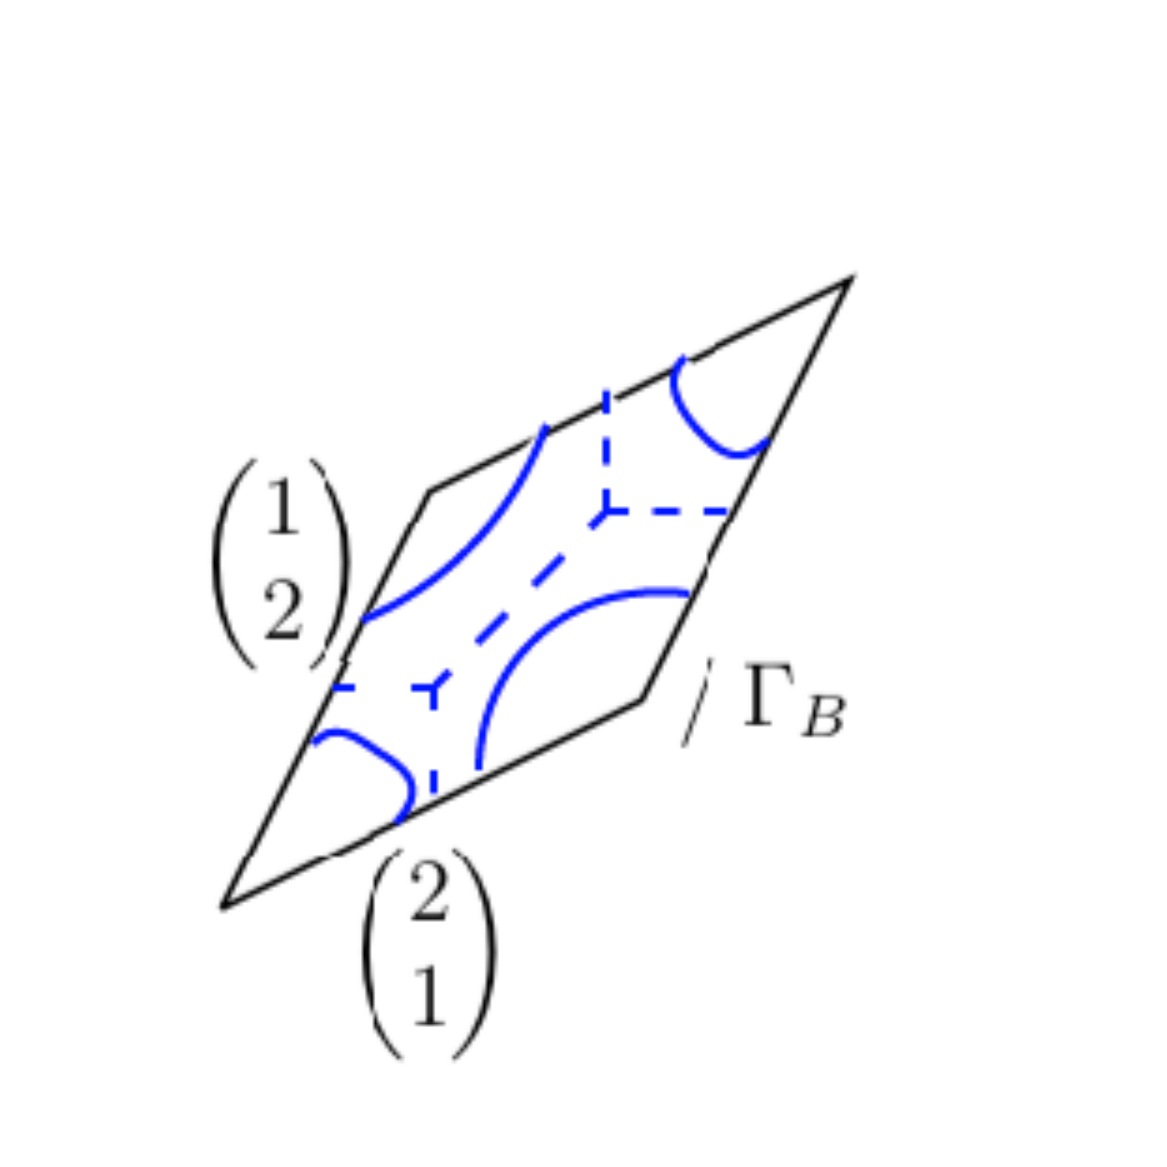
\includegraphics[width=0.42\textwidth]{figures/fig_1_1.png}
\caption{按 $\Gamma_B$ 取商（原书 p.11）}\label{fig:1-1}
\end{figure}

\transnote{图中蓝实线是 $\tau$ 很小时 $s(x)=0$ 的位置，四条蓝弧在粘合对边后两两
相接；虚线是 $\tau\to0$ 的极限（热带曲线），即后文热带化讨论的雏形。
「旋转 $2\pi$」指把平行四边形的斜边方向转正。图内标注 $/\,\Gamma_B$ 与两个
列向量保留原样，不译。}

\begin{remark}\label{rem:lattice-choice}
上文选取的 $\Gamma_B$ 格产生图~\ref{fig:1-1} 中由水平与垂直线段组成的蓝曲线，
本文通篇使用它。换一组生成元会得到不同的图，但本文的方法应当相同。
\end{remark}

\medskip\noindent\textbf{$X$ 与 $H$ 上不变量的关系}\par

\begin{theorem}[{拉格朗日环面丛的构造，取自 [AAK16, §4]}]\label{thm:lagrangian-fibration}
回忆 $x=(x_1,x_2)$ 是 $V$ 上的周期坐标。设 $y\in\C$ 是 $\C$ 因子上的坐标，
$s\colon V\to\LL$ 是上文定义的函数。然后定义
\begin{equation}\label{eq:1-9}
\begin{aligned}
X &:= \mathrm{Bl}_{H\times\{0\}}V\times\C\subset\PP(\LL\oplus\OO)\\
  &= \operatorname{graph}[s(x):y]\\
  &= \bigl\{(x,y,[s(x):y])\in(\PP(\LL\oplus\OO)\to V\times\C)\bigr\}\\
  &= \bigl\{(x,y,[u:v])\mid s(x)v=yu\bigr\},
\end{aligned}
\end{equation}
它是 $V\times\C$ 上 $\PP^1$-丛 $\PP(\LL\oplus\OO)$ 的子集。断言是：$X$ 带有
拉格朗日环面丛。
\end{theorem}

\begin{proof}[证明想法]
环簇有自然的环面作用（其一条轨道在簇中稠密），这个环面作用经矩映射自然给出
拉格朗日环面丛。$y$ 坐标上还有 $S^1$ 旋转作用。在矩映射的底空间上作剪切与粘贴，
对应总空间的爆破，由此在 $X$ 上得到拉格朗日环面丛。\qedhere
\end{proof}

% ===== 原书 p.12 =====
\begin{lemma}\label{lem:critical-locus}
$H=\mathrm{Crit}(y)$。
\end{lemma}

\begin{proof}
零纤维是 $V$ 的真变换与例外除子的并。设 $p$ 是收缩映射（blow-down map）：
\[
p\colon X\to V\times\C,\qquad (x,y,(u:v))\mapsto(x,y).
\]
真变换（proper transform）的定义是
\[
\tilde V := \overline{p^{-1}(V\setminus H\times\{0\})}.
\]
几何上 $\tilde V$ 是 $V$ 的一份拷贝，即爆破中 $V$ 远离 $H$ 那部分的闭包，
它补全了 $V$ 拷贝的其余部分。再定义由收缩映射在 $H$ 上给出的 $\PP^1$-丛，
以及该丛的一个截面 $s^p$：
\begin{align*}
\text{例外除子 } E &:= \{(x,0,(u:v))\mid x\in H\}=p^{-1}(H\times\{0\})\\
p|_E &\colon E\to H\times\{0\}\\
s^p &\colon H\to E,\qquad s^p(x) := (x,0,(1:0)).
\end{align*}
现在可把 $H$ 看成 $y$ 纤维丛的临界轨迹，即旋转 $y$ 的 $S^1$-作用的不动点集，
该作用为 $(x,e^{i\theta}y,(e^{-i\theta}u:v))$。
\begin{align*}
y^{-1}(0) &= \{(x,0,(u:v))\mid s(x)v=0\cdot u\}\\
&= \{(x,0,(1:0))\}\cup\{(x,0,(u:v))\mid s(x)=0\}\\
&= \tilde V\cup E.
\end{align*}
断言是 $\tilde V$ 与 $E$ 交于 $s^p(H)\cong H$。属于 $E$ 意味着 $s(x)=0$，
故 $x\in H$。属于 $\tilde V$ 意味着 $v=0$，故可把 $u\neq0$ 伸缩为 $u=1$。因此
\[
\tilde V\cap E=s^p(H)\cong H=\mathrm{Crit}(y).\qedhere
\]
\end{proof}

\medskip\noindent\textbf{辛不变量}\par

\begin{remark}\label{rem:dim1}
若 $\dim_{\C}V=1$，则 $y\colon X\to\C$ 的零纤维涉及形如 $ab=0$ 的正规交叉除子，
由维数原因产生一个 Lefschetz 奇点。于是可用 Seidel 的 Lefschetz 纤维丛的深谷范畴
[Sei08]；此时 $H$ 是一个点。我们想要该深谷范畴的类比，以 $H=\Sigma_2$ 为临界轨迹，
这需要升高一维。
\end{remark}

\begin{proposition}[{提出 Morse--Bott 纤维丛的深谷范畴 [AAK16]}]\label{prop:morse-bott}
$H\times0$ 在 $V\times\C$ 中的法丛是 $\LL\oplus\OO$。沿 $H\times\{0\}$ 爆破后，
$H=\Sigma_2$ 是正规交叉奇点中两个除子的交，并构成 Morse--Bott 纤维丛
$y\colon(x,y,(u:v))\mapsto y$ 的临界轨迹。于是 [AAK16, Corollary 7.8] 猜想
$\mathrm{Fuk}(H)$ 等价于 AAK 所描述的深谷范畴 $F_s(X,y)$，
因为 $H$ 中的拉格朗日可以从中纤维平行移动，得到 $X$ 中关于超势 $y$ 可容的
非紧拉格朗日。
\end{proposition}

\transnote{Lefschetz 纤维丛的临界点是孤立的；Morse--Bott 纤维丛的临界轨迹 $H$ 是
正维数的子流形，法丛的负特征值方向沿 $H$ 整体存在。这正是本文能用
$H=\Sigma_2$ 作临界轨迹、并把 $H$ 中的拉格朗日平行移动到 $X$ 中的原因。}

% ===== 原书 p.13 =====
\medskip\noindent\textbf{复不变量}\par

$X$ 与 $H$ 上有界相干层导出范畴的关系如下。

\begin{lemma}[{Orlov [APS]}]\label{lem:orlov}
存在半正交分解
\[
\DBCoh(X)=\bigl\langle\DBCoh(H),\DBCoh(V\times\C)\bigr\rangle.
\]
\end{lemma}

\transnote{半正交分解
$\DBCoh(X)=\langle\DBCoh(H),\DBCoh(V\times\C)\rangle$ 说明 $X$ 的导出范畴由
$H$ 与 $V\times\C$ 两块拼成，这是 Orlov 关于爆破的定理。后文用它在 $H$ 一侧
构造嵌入，$V\times\C$ 一侧用线丛处理。}

\medskip\noindent\textbf{对亏格 2 曲线选取的依赖}\par

\begin{claim}\label{claim:embed-genus2}
任何亏格 $2$ 曲线都能嵌入复维数 $2$ 的阿贝尔簇。
\end{claim}

\begin{proof}
固定一点 $x_0\in\Sigma_2$，则映射
$\Sigma_2\ni x\mapsto\OO(x-x_0)\in\mathrm{Pic}^0(\Sigma_2)$ 是单射
[Huy05, Proposition 2.3.34]。而 $\mathrm{Pic}^0(\Sigma_2)$ 同构于 $\Sigma_2$ 的
Jacobi 簇，后者是阿贝尔簇，见 [For91, §21.7]。具体地，设
$\{\omega_1,\omega_2\}\in H^{1,0}(\Sigma_2)$ 是一组基，取
$\alpha_1,\dots,\alpha_4\in H_1(\Sigma_2;\Z)$ 为同调的一组基。设 $c$ 是 $\Sigma_2$
上的链，使 $\partial c=x-x_0$。则嵌入为
\[
\Sigma_2\ni x\mapsto\Bigl(\int_c\omega_1,\int_c\omega_2\Bigr)
\in\operatorname{Jac}(\Sigma_2)=\C^2/\operatorname{Per}(\omega_1,\omega_2),
\]
其中
$\operatorname{Per}(\omega_1,\omega_2)
:=\Z\bigl\{\bigl(\int_{\alpha_i}\omega_1,\int_{\alpha_i}\omega_2\bigr)\bigr\}_i$。

注意：把 $\mathrm{Pic}(\Sigma_2)$ 定义为全纯线丛 [Huy05]，与定义为除子模主除子
[For91, §21.6]，两种定义等价。理由是：任何复曲线都能用适当高次线丛的截面嵌入
射影空间 [For91, Theorem 17.22]；因此映射
$\mathrm{Div}(\Sigma_2)\ni D\mapsto\OO(D)\in\mathrm{Pic}(\Sigma_2)$ 是满射
[Huy05, Corollary 5.3.7]。
\end{proof}

\begin{corollary}\label{cor:vary-genus2}
改变亏格 $2$ 曲线，对应改变 $V$（因而改变 $X$）的复结构参数。复结构极限在镜像
映射中有计数意义，见 [CLL12]。所以经镜像映射，这也改变 $Y$ 的凯勒参数。
\end{corollary}

% EN48 c02 | 原书 p.13 中部–p.23 上部（PDF 22–32） | 第 1 章 §1.3
% 块骨架：标题行已设定，正文由译者填写。每页起首用 % ===== 原书 p.N ===== 注释标记。
% 边界说明：按 Lead 批复的方案 A，本块收 §1.3 的全部 30 条结果（自本条首的定义至末条注），
% 止于原书 p.23 上部的末条注；§1.4 自 p.23 中部起，归 c03。
\subsection{环簇的背景}

% ===== 原书 p.13 =====
SYZ 镜像 $Y$ 的构造用到环簇这一套工具：先得到簇 $\tilde Y$，再令
$Y := \tilde Y/\Gamma_B$。环簇提供一种组合式的办法，用来产生定义流形所需的
坐标卡与过渡函数。

下文要在 $Y$ 上定义辛形式。这是给 $Y$ 配备深谷范畴、再用该范畴证明 HMS 的第一步。
% ===== 原书 p.14 =====
由于 $Y$ 局部上是环簇 $\tilde Y$ 按离散群取商的结果，而由多面体构造出的环簇天然
带有线丛，我们就用该线丛的截面定义一个度量。这个度量将给出辛形式。

我们先建立定义该线丛所需的理论。下面是行动路线。
\begin{center}
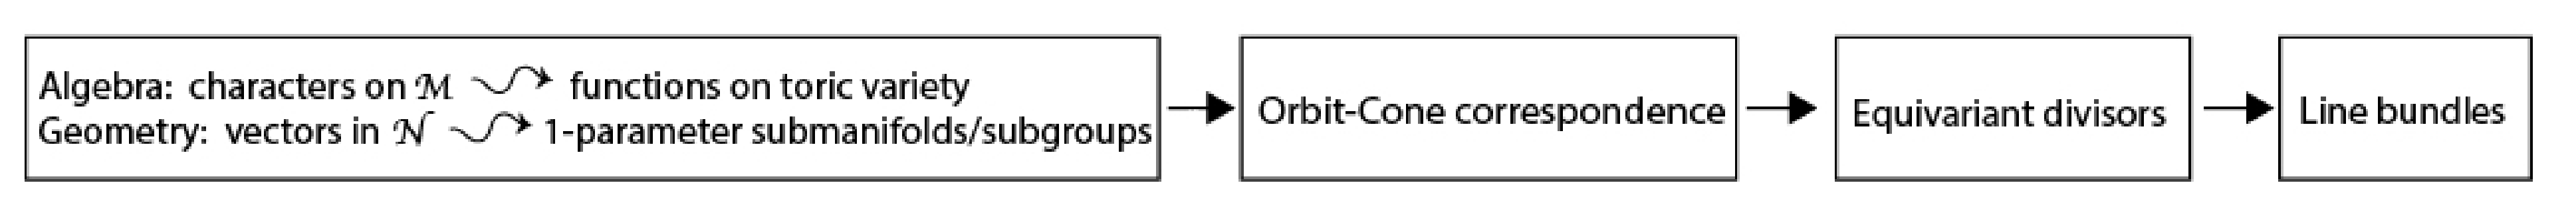
\includegraphics[width=0.98\textwidth]{figures/fig_c02_plan.png}
\end{center}
本小节的背景取自 [CLS11, p 59, p128] 与 [Ful93, Chapter 1]。

\transnote{上图把本节要建立的两条线索并排列出：左栏是代数侧，$M$ 中的特征标给出
环簇上的函数；左栏下一行是几何侧，$N$ 中的向量给出单参数子群。中栏到右栏是推导
路线：先证轨道–锥对应，再由它得到等变除子，最后由除子得到线丛。}

\medskip\noindent\textbf{特征标与单参数子群}\par

设 $Y_\Delta$ 为与多面体 $\Delta$ 相伴的环簇，其构造下文说明。本文对
$Y_\Delta = \PP^2(3)$（即 $\PP^2$ 在三点处爆破）以及后文描述的另一个无限型环簇
[KL19] 使用这套理论。轨道–锥对应解释组合数据（锥）如何给出几何数据（轨道）。
这些数据分别编码在两个向量空间里：特征标空间 $M_\R$，其元素是 $Y_\Delta$ 上的
函数；以及「余特征标」空间 $N_\R$，它生成 $Y_\Delta$ 中的单参数子群（PS）。
下标 $\R$ 表示把格与 $\R$ 作张量积。在这个环簇的代数几何设定里，$M$ 是「代数」，
$N$ 是「几何」。

\begin{definition}[记号]\label{def:notation}
我们固定一些记号。下文将考虑 $n=2$ 与 $n=3$ 的例子。
\begin{itemize}[leftmargin=2.2em,itemsep=0.25em]
\item 几何：$N := \Z^n$，其向量编码环面 $T_N := (\C^*)^n$ 中由 $\C^*$ 参数化的
  单参数子群；该环面在环簇中稠密。有 $N\otimes_\Z\C^* = T_N$ 与
  $N_\R := N\otimes_\Z\R$。
\item 代数：$M = \Hom_\Z(N,\Z)$ 同时编码 $N$ 上的线性泛函（组合层面）与环簇上的
  函数（流形层面）。在 [AAK16] 中，$M$ 的元素称为权向量，因为将其指数化得到
  环簇单项式，而后者是特征标，即环簇上的函数。
\item $M_\R = \R^n$，并由 $\ip{e_i}{f_j} = f_j(e_i) = \delta_{ij}$ 定义非退化配对
  $M_\R\times N_\R\to\R$。
\end{itemize}
\end{definition}

\begin{definition}[锥]\label{def:cone}
锥 $\sigma\subset N_\R$ 是一族半空间
$H_u^+ := \{n\in N_\R\mid \ip{u}{n}\ge 0\}$ 的交，其中 $u$ 取遍 $M$ 中一组法向量。
例如取 $u_1 = e_1$、$u_2 = e_2$，就得到第一象限 $e_1,e_2\ge 0$。于是 $\sigma$ 由
若干格向量的凸线性组合构成；这些格向量称为射线 $\rho$，其全体记作 $\sigma(1)$。

对偶锥 $\sigma^\vee\subset M_\R$ 定义为对偶半空间的交：
\[
\sigma^\vee := \{m\in M_\R\mid \ip{m}{n}\ge 0\ \forall n\in\sigma\}
= \bigcap_{n\in\sigma(1)}\{m\in M_\R\mid \ip{m}{n}\ge 0\}.
\]
\end{definition}

% ===== 原书 p.15 =====
\begin{definition}[强凸有理多面体锥]
强凸指 $\sigma$ 不由任何方向 $e$ 上的 $\pm e$ 生成（等价地，
$\sigma\cap(-\sigma)=\{0\}$）；有理指 $\sigma$ 有整生成元，即生成元都在 $\Z^n$ 中。
\end{definition}

\begin{remark}
若 $m_1,\dots,m_s$ 生成 $\sigma^\vee$，则它们就是 $\sigma$ 中那些半空间的法向量，
即 $\sigma = H_{m_1}^+\cap\cdots\cap H_{m_s}^+$。于是要点在于：$\sigma^\vee$ 把这些
法向量整体编码起来，它的边是 $\sigma$ 的刻面。更一般地，$\sigma$ 中的面 $\tau$
对应 $\sigma^\vee$ 中一个维数互补的面，记作 $\tau^*$，即
$\tau^\perp\cap\sigma^\vee$；反之亦然。
\end{remark}

\transnote{这里「它的边是 $\sigma$ 的刻面」是对偶关系，不是说两者是同一族子集：
$\sigma$ 的刻面（余维 $1$ 的面）与 $\sigma^\vee$ 的边（1 维面）一一对应，且
$\dim\tau + \dim\tau^* = n$。读后文关于多面体刻面的定义时，可以回头对照这一条。}

\begin{definition}[特征标]\label{def:character}
令 $S_\sigma := \sigma^\vee\cap M$ 为对偶锥中的格点。坐标环 $\C[S_\sigma]$ 的元素是
局部定义在 $Y_\Delta$ 上的函数，称为特征标或环簇单项式。它们是集合
$\{\chi^u\mid u\in S_\sigma\}$ 中元素的 $\C$-线性组合。在环簇上定义开集
\[
U_\sigma := \operatorname{Spec}\C[S_\sigma].
\]
特别地，由于 $S_\sigma$ 是半群（可以相加，且含零元），元素 $\chi^u$ 的集合具有
自然的环结构，符合我们对函数坐标环的预期。
\end{definition}

\begin{remark}[记号]
我们用字母 $u$ 表示 $N$ 中的格点。字母 $m$ 保留给 $M_\R$ 或 $M$ 中的点，$n$ 表示
$N_\R$ 中的元素。这样做与 [CLS11] 一致。
\end{remark}

\begin{definition}[仿射卡与函数]\label{def:affine-chart}
$Y_\Delta$ 上的仿射卡（或局部卡）是 $\operatorname{Spec}\C[S_\sigma]$。特别地，
所有局部卡都包含稠密环面
$(\C^*)^n = \operatorname{Spec}\C[\chi^{\pm e_1},\dots,\chi^{\pm e_n}]$，因为
\[
M = \operatorname{Span}_{\Z_+}\langle \pm e_1,\dots,\pm e_n\rangle
\supset \{u\in\sigma^\vee(1)\},
\]
并且射线生成半群 $S_\sigma$。局部函数由特征标 $\chi^u$ 给出。特征标是从稠密环面
到 $\C^*$ 的同态：
\[
\chi^u\colon(\C^*)^n\to\C^*,\qquad
(t_1,\dots,t_n)\mapsto t^u := t_1^{u_1}\cdots t_n^{u_n},\qquad
u = \sum_{i=1}^n u_i e_i.
\]
固定 $S_\sigma$ 的一组基 $\{u_1,\dots,u_k\}$，意思是
$\{\pm u_1,\dots,\pm u_l,u_{l+1},\dots,u_k\}$ 在 $\Z_+$ 上生成 $S_\sigma$，且
$\{u_1,\dots,u_k\}$ 之间没有关系（即极小生成元）。若 $\sigma$ 是强凸锥，就得到带
局部复坐标 $\chi^{u_1},\dots,\chi^{u_k}$ 的坐标卡：
\[
(\chi^{u_1},\dots,\chi^{u_k})\colon U_\sigma\to\C^k.
\]
\end{definition}

\transnote{第一行的包含关系里，$\operatorname{Span}_{\Z_+}\langle
\pm e_1,\dots,\pm e_n\rangle$ 其实就是整个 $M$（因为允许 $\pm e_i$，$\Z_+$ 系数
等于 $\Z$ 系数）。所以任何一张仿射卡都含稠密环面，卡与卡之间的差别只在额外加了
哪些 $\chi^u$。集合 $\sigma^\vee(1)$ 指对偶锥的射线（1 维面）的生成元。}

\begin{remark}
这个卡的像可能是 $\C^k$ 中一个可能奇异的 $n$ 维子簇。特别地，对极大锥有 $k=n$，
$u_i$ 构成 $M$ 的一组 $\Z$-基，于是得到一个光滑簇，以及通常意义上的仿射流形卡，
它把 $U_\sigma$ 映到
% ===== 原书 p.16 =====
局部模型 $\C^n$。

另一种情形是 $u_i$ 不构成 $M$ 的 $\Z$-基，此时它们之间有关系。具体地，
\[
\C[S_\sigma]\cong \C[\chi^{u_1},\dots,\chi^{u_k}]/I,
\]
其中 $I$ 是记录这些关系的环簇理想。下文的 $\PP^2$ 例子（例~\ref{ex:cp2-fan}）
不需要对环簇理想取商。

适当取这个卡的闭包即得环簇。后文会考察特征标何时延拓为整个环簇上的函数，
即 $(\C^*)^n$ 的部分或完全紧化：我们让坐标趋于 $0$ 或无穷。这说明了 $M$ 如何
产生函数。
\end{remark}

\begin{definition}[环簇]\label{def:toric-variety}
回忆锥 $\sigma$ 给出仿射卡。扇是一族锥，其排列方式告诉我们如何粘合局部卡，
即流形上的过渡函数是什么。扇是 $N_\R$ 中的一族锥 $\sigma_i$，满足
\begin{itemize}[leftmargin=2.2em,itemsep=0.25em]
\item 每个锥的每个面都是锥；
\item $\tau_{ij} := \sigma_i\cap\sigma_j$ 是 $\sigma_i$ 与 $\sigma_j$ 共同的面，
  因此沿 $U_{\tau_{ij}}$ 把 $U_{\sigma_i}$ 与 $U_{\sigma_j}$ 粘合。
\end{itemize}
设 $\sigma_1,\sigma_2$ 是两个极大锥，使 $\tau = \sigma_1\cap\sigma_2$ 为 $(n-1)$ 维。
\end{definition}

\begin{claim}\label{claim:tau-hyperplane}
$\tau = H_m\cap\sigma_1 = H_m\cap\sigma_2$，其中
$m\in\sigma_1^\vee\cap(-\sigma_2)^\vee\cap M$。
\end{claim}

特别地，半群 $S_\tau$ 现在含 $\pm m$ 两个方向，而 $\sigma_1$ 只含 $m$、$\sigma_2$
只含 $-m$。这相当于在第一张卡 $\C[S_{\sigma_1}]$ 中把坐标 $\chi^m$ 取逆、在第二张卡
$\C[S_{\sigma_2}]$ 中把坐标 $\chi^{-m}$ 取逆；两者现在都要求非零。我们沿
\[
U_\tau = (U_{\sigma_1})_{\chi^m} = (U_{\sigma_2})_{\chi^{-m}}
\]
粘合这两张卡。

\transnote{两张卡各自的坐标是 $\chi^m$ 与 $\chi^{-m}$，它们互为倒数；要求非零就是
要求取出这两张卡的交。后文例~\ref{ex:cp2-fan} 的过渡映射 $g_{12}$ 正是把这个取逆写成坐标
变换，即 $\chi^{(1,0)}\mapsto 1/\chi^{(1,0)}$。}

由此可以看出 $N$ 如何产生单参数子群。

\begin{definition}[单参数子群（1-PS）]\label{def:one-parameter}
给定 $v = \sum_{i=1}^n v_i f_i\in N$，通过乘法同态得到单参数子群 $\lambda^v$：
\[
\lambda^v\colon \C^*\to(\C^*)^n,\qquad t\mapsto(t^{v_1},\dots,t^{v_n}).
\]
例如 $v=(1,1)$ 给出复单参数子群 $(t,t)_{t\in\C^*}\subset(\C^*)^2$。取
$(\chi^{u_1},\dots,\chi^{u_k})$ 在 $\{\lambda^v(t)\}_{t\in\C^*}$ 上的像，
就得到 $U_\sigma$ 中的一维子流形。
\end{definition}

\begin{remark}
把特征标与单参数子群复合，得到 $\C^*$ 的特征标：
\[
\chi^u\circ\lambda^v(t) = t^\ell,\qquad \ell = \ip{u}{v}.
\]
特别地，把所有单参数子群收集起来，即可几何地看出 $N$ 就是稠密环面：
\[
N\otimes_\Z\C^*\colon v\otimes t\mapsto\lambda^v(t).
\]
\end{remark}

% ===== 原书 p.17 =====
\begin{example}[$\PP^2$]\label{ex:cp2-fan}
扇有三个锥，其射线分别由 $v_1 = f_1$、$v_2 = f_2$、$v_3 = -f_1-f_2$ 在 $N_\R$
中生成。
\begin{center}
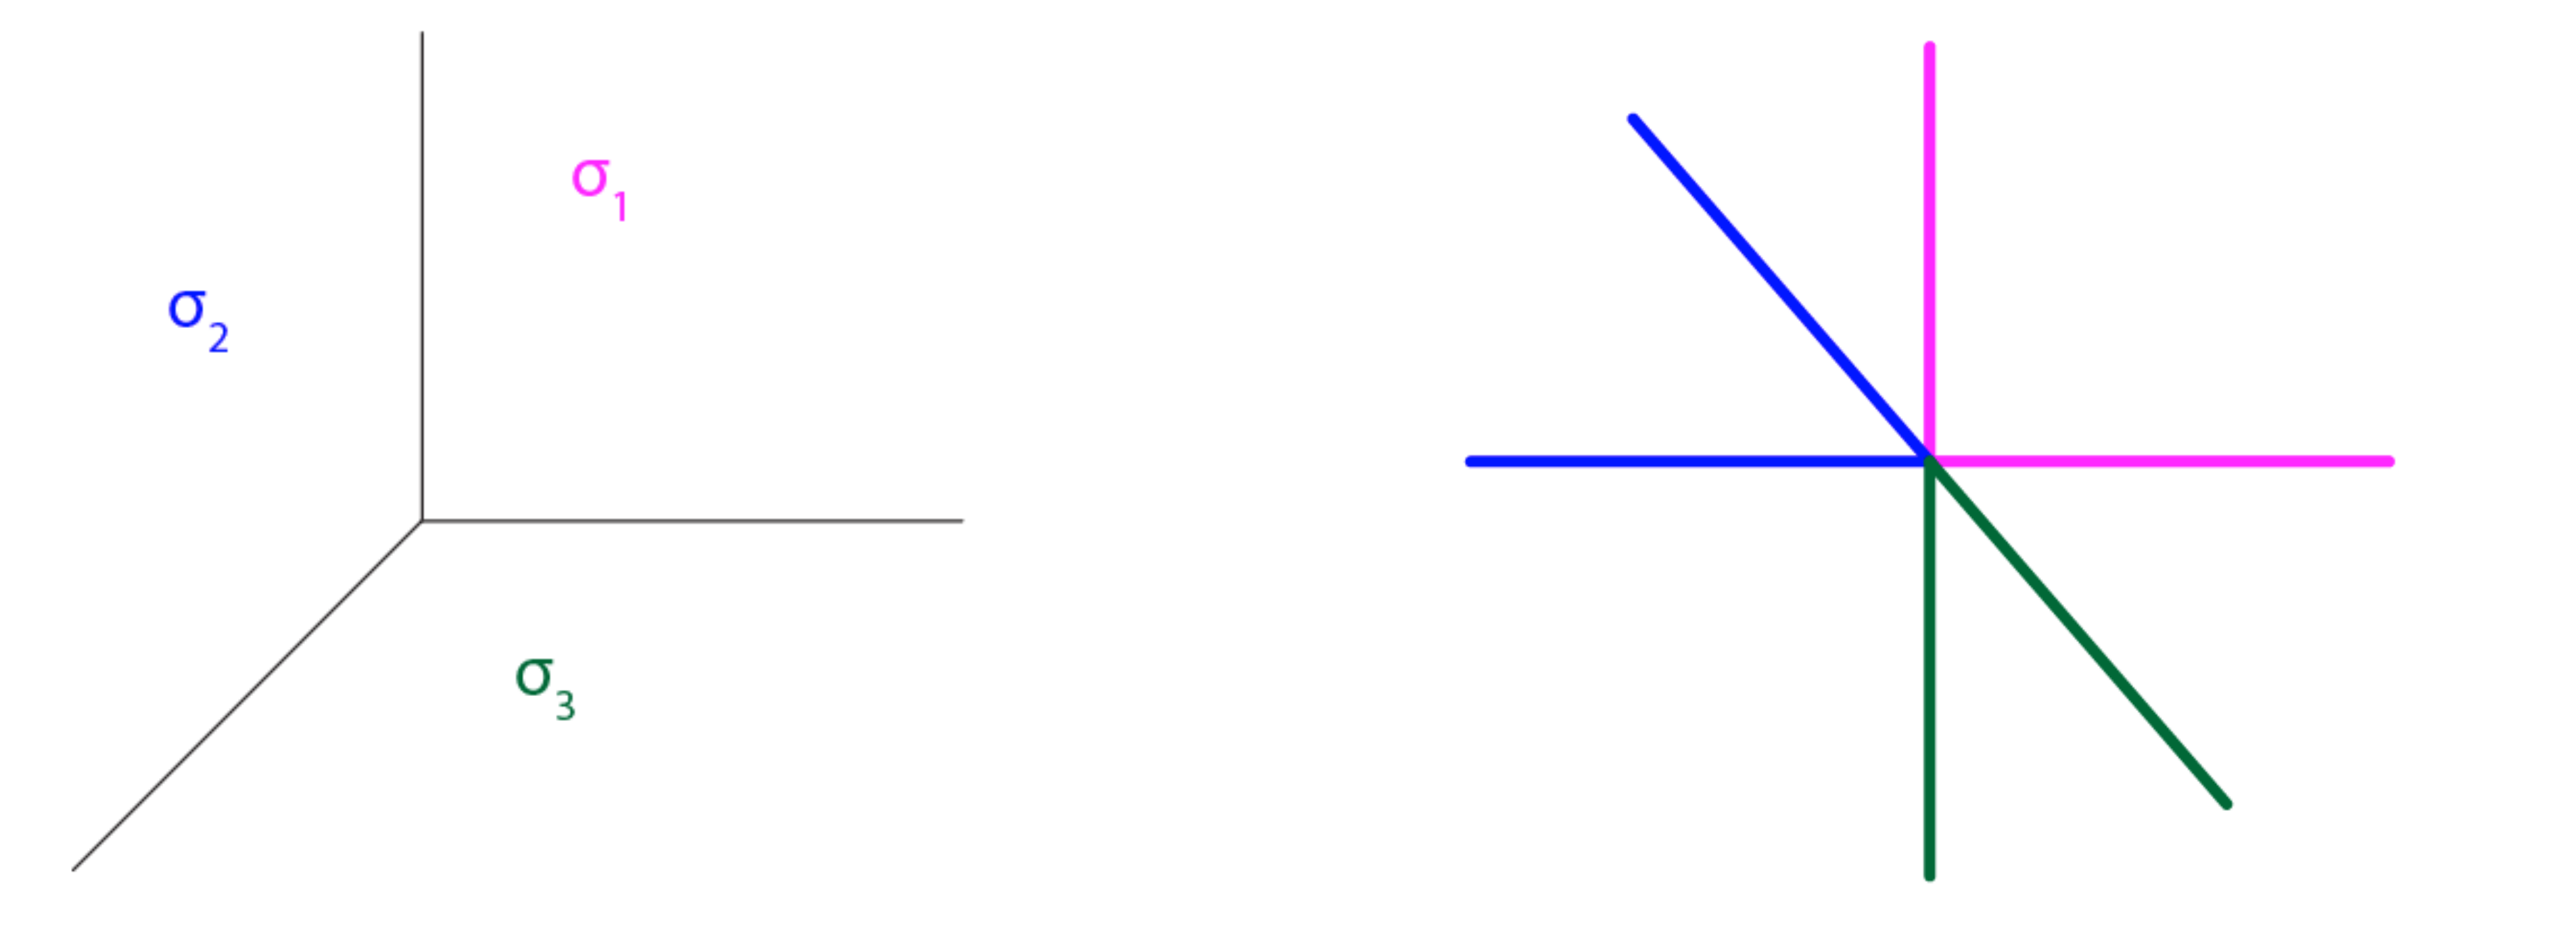
\includegraphics[width=0.86\textwidth]{figures/fig_c02_fan.png}
\end{center}
在原锥上取非负值的线性泛函，其对偶锥为
\begin{gather*}
\sigma_1^\vee = \operatorname{span}(e_1,e_2),\\
\sigma_2^\vee = \operatorname{span}(-e_1,-e_1+e_2),\\
\sigma_3^\vee = \operatorname{span}(-e_2,e_1-e_2).
\end{gather*}
这些对中的向量之间没有关系，所以它们对应某个同构于 $\C[x,y]$ 的仿射卡的变量。
换言之，我们不需要对记录生成元之间关系的环簇理想 $I$ 取商。每种情况下选取生成元，
就给出卡上的一个复坐标。
\begin{align*}
U_{\sigma_1} &= \operatorname{Spec}\C[\chi^{1,0},\chi^{0,1}]\cong\C^2
\ni(\chi^{1,0},\chi^{0,1}),\\
U_{\sigma_2} &= \operatorname{Spec}\C[\chi^{-1,0},\chi^{-1,1}]\cong\C^2
\ni(\chi^{-1,0},\chi^{-1,1}),\\
U_{\sigma_3} &= \operatorname{Spec}\C[\chi^{0,-1},\chi^{1,-1}]\cong\C^2
\ni(\chi^{0,-1},\chi^{1,-1}).
\end{align*}
若 $\tau = \sigma_1\cap\sigma_2$，则这相当于把 $\chi^{1,0}$ 取逆，并且
$\tau^\vee = H^+_{(1,0)}$。选定生成元就选定了坐标；两种不同的自然选择给出坐标变换：
\begin{align*}
\C[S_{\sigma_1}] &= \C[\chi^{(1,0)},\chi^{(0,1)}]
\subset \C[\chi^{\pm(1,0)},\chi^{(0,1)}] = \C[S_\tau]\\
&\rightsquigarrow \operatorname{Spec}\C[\chi^{\pm(1,0)},\chi^{(0,1)}]
\to \operatorname{Spec}\C[\chi^{(1,0)},\chi^{(0,1)}],
\end{align*}
以及
\begin{align*}
\C[\chi^{-(1,0)},\chi^{(-1,1)}] &\subset
\C[\chi^{\pm(1,0)},\chi^{(-1,1)}]\\
&\rightsquigarrow \operatorname{Spec}\C[\chi^{\pm(1,0)},\chi^{(-1,1)}]
\to \operatorname{Spec}\C[\chi^{-(1,0)},\chi^{(-1,1)}].
\end{align*}
注意 $\C[\chi^{\pm(1,0)},\chi^{(0,1)}] = \C[\chi^{\pm(1,0)},\chi^{(-1,1)}]$，
在 $\operatorname{Spec}$ 下得到 $U_\tau$。选定生成元给出与 $\C^*\times\C$ 的一个
等同；两张卡中的这个等同再作为恒等映射嵌入 $\C^2$。这个等同的两种不同选择给出
过渡映射：
\[
g_{12}(\chi^{(1,0)},\chi^{(0,1)}) :=
\left(\frac{1}{\chi^{(1,0)}},\ \frac{\chi^{(0,1)}}{\chi^{(1,0)}}\right).
\]
这样就回到我们对 $\PP^2\ni[z_0:z_1:z_2]$ 的理解，其中
$\chi^{(1,0)} = z_1/z_0$，$\chi^{(0,1)} = z_2/z_0$。
\end{example}

\transnote{两串包含与 $\operatorname{Spec}$ 的图说的是同一件事：$U_{\sigma_1}$ 与
$U_{\sigma_2}$ 各自嵌入 $U_\tau$，而 $U_\tau$ 等同 $\C^*\times\C$。把第二串的坐标
换回第一串的坐标就得到 $g_{12}$，这正是 $\PP^2$ 的标准过渡函数：$\C^*\times\C$
里一点在第一张卡上记作 $(\chi^{(1,0)},\chi^{(0,1)})$，在第二张卡上记作其倒数。}

% ===== 原书 p.18 =====
\medskip\noindent\textbf{轨道–锥对应}\par

要理解等变除子，需要理解组合数据如何给出几何数据。除子对应簇上某个坐标的零点。
这一点可以从扇通过「轨道–锥对应」读出。

\begin{lemma}[轨道–锥对应]\label{lem:orbit-cone}
环簇中某点的 $n-k$ 维 $(\C^*)^n$-轨道，与扇的 $k$ 维锥之间存在一一对应；
例如除子与射线对应。
\end{lemma}

\begin{proof}
思路是：「对应于 $N$ 中某个锥内部的点的每个单参数子群，都收敛到同一个极限点。」
（回忆定义~\ref{def:one-parameter} 中 $N$ 的点与单参数子群的对应。）该点给出确定
单参数子群方向的向量。按代数几何，环簇上的一个点是半群同态
$S_\sigma = \C[\sigma^\vee\cap M]\to\C$，即映射
$\operatorname{Spec}\C\to U_\sigma$。回忆 $M$ 编码环簇上的函数。因此，这样的赋值
确定了所有函数在该点的取值；知道一个点处所有函数的取值，与知道这个点本身是同样的
信息。给定 $v\in\sigma\cap N$，用 $\sigma^\vee\cap M$ 的一组基上的如下映射，可以给
相应的点指定坐标：
\[
\sigma^\vee\cap M\ni u\mapsto\lim_{t\to0}\chi^u(\lambda^v(t))
= t^{\ip{u}{v}}\in\C.
\]
下面用一条断言说明：一个锥的所有向量为何给出同一个极限点。由此，取该锥的极限点
的轨道，就得到轨道–锥对应。

\begin{claim}\label{claim:limit-point}
由方向 $v\in\operatorname{int}(\sigma)\cap N$ 给出的所有单参数子群都收敛到同一点。
\end{claim}

\begin{proof}
为清楚起见，我们用下标 $u_{\mathrm{bdry}}$、$u_{\mathrm{int}}$ 区分需要对每个 $v$
核对的两种函数（即 $u$ 不在对偶锥 $\sigma^\vee\subset M$ 的内部，或 $u$ 在其内部）。
可以看到：
\begin{enumerate}[leftmargin=2.6em,itemsep=0.3em]
\item $u_{\mathrm{bdry}}\in\sigma^\vee\cap\sigma^\perp$ 推出对一切 $v\in\sigma$ 有
  $\ip{u_{\mathrm{bdry}}}{v}=0$，因此
  \[
  \lim_{t\to0}\chi^u(\lambda^v(t)) = t^{\ip{u}{v}} = 1.
  \]
\item $u_{\mathrm{int}}\in\sigma^\vee\setminus(\sigma^\vee\cap\sigma^\perp)$ 推出：
  一方面，按 $\sigma^\vee$ 的定义，对一切 $v\in\operatorname{int}(\sigma)\cap N$
  有 $\ip{u_{\mathrm{int}}}{v}\ge 0$；另一方面，对 $\sigma$ 内部的 $v$ 有
  $\ip{u_{\mathrm{int}}}{v}\ne 0$，且 $u_{\mathrm{int}}\notin\sigma^\perp$。因此
  \[
  \lim_{t\to0}\chi^u(\lambda^v(t)) = t^{\ip{u}{v}} = 0.
  \]
\end{enumerate}
\end{proof}

为完成轨道–锥对应的证明，令对应锥 $\sigma$ 的轨道为 $(\C^*)^n\cdot p$，其中 $p$
是点
\[
\lim_{t\to0}\bigl(\chi^{u_1}(\lambda^v(t)),\dots,
\chi^{u_k}(\lambda^v(t))\bigr),
\]
$v\in\sigma$，$u_1,\dots,u_k$ 是 $S_\sigma$ 的生成元。由上一条断言，可以任取 $v$。
\end{proof}

\transnote{两个极限的差别全在指数 $\ip{u}{v}$ 上：边界方向使指数为 $0$，极限是
$1$；内部方向使指数严格为正，极限是 $0$。所以「极限点」的各坐标只取 $0$ 或 $1$，
由 $u$ 属于哪一类函数决定。这也解释了为何同一锥的所有方向给出同一点。}

% ===== 原书 p.19 =====
\begin{example}[$\PP^2$]\label{ex:cp2-cones}
扇的锥与对偶锥如下：
\begin{gather*}
\{0\},\quad \{0\}^\vee = M_\R\cong\R^2,\\
\rho_1 = \langle(1,0)\rangle,\quad \rho_2 = \langle(0,1)\rangle,\quad
\rho_3 = \langle(-1,-1)\rangle,\\
\rho_1^\vee = \langle\pm(0,1),(1,0)\rangle,\quad
\rho_2^\vee = \langle\pm(1,0),(0,1)\rangle,\\
\rho_3^\vee = \langle\pm(-1,1),(-1,0)\rangle,\\
\sigma_1 = \langle(1,0),(0,1)\rangle,\quad
\sigma_2 = \langle(1,0),(-1,-1)\rangle,\quad
\sigma_3 = \langle(0,1),(-1,-1)\rangle,\\
\sigma_1^\vee = \langle(1,0),(0,1)\rangle,\quad
\sigma_2^\vee = \langle(0,1),(1,-1)\rangle,\\
\sigma_3^\vee = \langle(-1,0),(-1,1)\rangle.
\end{gather*}
生成与锥 $\sigma$ 对应的轨道的极限点 $\gamma_\sigma$，是把
$\sigma^\perp\cap\sigma^\vee$ 中的向量 $m$ 送到 $1$、把 $\sigma^\vee$ 中其余向量
送到 $0$ 的点。令 $(t_1,t_2)\in(\C^*)^2$ 为稠密环面轨道上的坐标。对 $S_{\rho_i}$
所取的生成元列在下面的指数中。
\begin{align*}
\lambda^{(0,0)}(t) &= (1,1), &
\gamma_{\{0\}} &= \lim_{t\to0}(\chi^{(1,0)}(1,1),\chi^{(0,1)}(1,1))
= (1,1) \Longrightarrow (\C^*)^2,\\
\lambda^{(1,0)}(t) &= (t,1), &
\gamma_{\rho_1} &= \lim_{t\to0}(\chi^{(0,1)}(t,1),\chi^{(1,0)}(t,1))
= (1,0) \Longrightarrow \C^*\times\{0\},\\
\lambda^{(0,1)}(t) &= (1,t), &
\gamma_{\rho_2} &= \lim_{t\to0}(\chi^{(1,0)}(1,t),\chi^{(0,1)}(1,t))
= (1,0) \Longrightarrow \C^*\times\{0\},\\
\lambda^{(-1,-1)}(t) &= (t^{-1},t^{-1}), &
\gamma_{\rho_3} &= \lim_{t\to0}(\chi^{(-1,1)}(t^{-1},t^{-1}),
\chi^{(-1,0)}(t^{-1},t^{-1})) = (1,0) \Longrightarrow \C^*\times\{0\}.
\end{align*}
在环簇中取闭包，就得到三个环簇除子，即 $(\C^*)^n$ 作用不变的除子。
\end{example}

\transnote{表中每行左边是单参数子群 $\lambda^v$，右边是它给出的极限点。第三、四行的
第一分量都趋于 $1$，第二分量都趋于 $0$，所以轨道是 $\C^*\times\{0\}$ 型的一维轨道。
$\gamma_{\{0\}}$ 对应零锥，它的轨道就是整个稠密环面 $(\C^*)^2$。}

\begin{claim}\label{claim:orbit-closure}
设 $O(\sigma)$ 表示轨道–锥对应下与锥 $\sigma$ 对应的轨道。则轨道的闭包给出的
环簇除子有如下描述：
\[
\overline{O(\tau)} = \bigcup_{\tau\le\sigma} O(\sigma).
\]
\end{claim}

记号：$N(\sigma)$ 指 $N$ 中的格点模去 $N_\sigma$ 中的格点，其中
$N_\sigma := \sigma\cap N$。

\medskip\noindent\textbf{除子、线丛与多面体}\par

除子–射线对应是轨道–锥对应的特例；按复几何 [Huy05, §2.3]，除子的定义函数给出
线丛的过渡函数。下面引入多面体的概念，并说明它为何决定一个线丛。我们将看到，
它的构造使它的边与扇中的射线垂直，而它的大小控制每个不可约环簇除子（对应扇的
射线）上的系数。这个除子随后给出与该多面体对应的线丛。

\begin{definition}[多面体]\label{def:polytope}
多面体 $P\subset M_\R$ 是
\[
P := \{m\in M_\R\mid \ip{m}{\nu_i}\ge -a_i\}\subset M_\R,
\]
其中 $i$ 取有限多个值，$\nu_i\in N$ 生成扇 $\Sigma$ 的射线 $\rho_i$。若 $i$ 取
无限多个值，更一般地得到多面体（polyhedron）。
\end{definition}

% ===== 原书 p.20 =====
\begin{definition}[面、刻面]
多面体中余维 $1$ 的面称为刻面：对某个 $i$ 有 $\ip{u}{v_i} = -a_i$，且对 $j\ne i$
有 $\ip{u}{v_j} > -a_j$。余维更高的面则对不止一个 $i$ 满足
$\ip{u}{v_i} = -a_i$。
\end{definition}

% [Tutor Note: 本条原文用 v_i 与 u，与定义~\ref{def:polytope} 的 ν_i、以及记号约定中「m 表示
% 多面体侧的点」不一致。此处照录原书符号，不作改动。]

\begin{definition}[由 $P$ 得到扇]\label{def:fan-from-polytope}
（全维格多面体的顶点对应环簇卡，参见 [CLS11, p 76]。）给定顶点为 $\mathbf v$ 的
多面体 $P$，把每个顶点平移为原点，取它的边张成的锥，即
$C_{\mathbf v} := \operatorname{Cone}(P\cap M-\mathbf v)\subset M_\R$。对应的扇中的
锥定义为
\[
\sigma_{\mathbf v} := C_{\mathbf v}^\vee
= \operatorname{Cone}(\nu_i\mid \text{第 } i \text{ 个面包含 } \mathbf v)
\subset N_\R.
\]
于是卡为
$U_{\sigma_{\mathbf v}}
= \operatorname{Spec}\C[\operatorname{Cone}(P\cap M-\mathbf v)\cap M]$。（更一般地，
对多面体的面 $Q$，$\sigma_Q$ 是由包含 $Q$ 的面的 $\nu_i$ 张成的锥。）所以要点是：
「环簇的局部坐标可以从多面体的顶点出发沿它的边读出。」
\end{definition}

检查所有锥 $\sigma_Q$ 的全体确为一个扇，我们把它定义为 $\Sigma_P$。

\transnote{这里的操作分三步：先把多面体平移使某个顶点落在原点，再由该顶点出发的边
张成一个锥 $C_{\mathbf v}$；取对偶锥就落到 $N$ 一侧，得到扇的锥。对偶的作用正是把
「多面体的边」换成「法向量 $\nu_i$」。所以多面体的顶点对应扇的极大锥，而多面体的
面（法向量）对应扇的射线。}

\begin{remark}
关于对偶化 $\sigma\to\sigma^\vee$ 在多面体层面的类比（多面体 → 极多面体），讨论见
[Ful93, §1.5, p 26]。可以把 $M_\R$ 中的多面体 $P$ 过渡到锥
$\operatorname{Cone}(P\times\{1\})\subset M_\R\times\R$，再对锥取对偶 $\vee$，
得到 $N_\R\times\R$ 中的锥；可以证明这是 $P$ 的极 $P^0$ 上的锥，即形如
$\operatorname{Cone}(P^0\times\{1\})$，其中 $P^0\subset N_\R$ 是对偶多面体。
\end{remark}

\transnote{取 $\operatorname{Cone}(P\times\{1\})$ 相当于给多面体加一个高度坐标，
把有界的多面体变成无界的锥；锥的对偶仍在锥的层面进行，所以「多面体对偶」被化归为
「锥对偶」。这与定义~\ref{def:cone} 的对偶锥是同一套操作，只是所在空间多了一维。}

\begin{definition}[等变除子]
等变除子（或 $T$-除子）是环簇轨道闭包的线性组合。
\end{definition}

\begin{claim}
$T$-除子是刻面对应除子的线性组合。
\end{claim}

\begin{proof}
扇的射线对应等变除子。事实上，给定射线 $\rho$，其正交补 $\rho^\perp$ 余维为 $1$；
这意味着特出点 $\gamma_\rho$ 有 $n-1$ 个 $1$ 与 $1$ 个 $0$（其中 $0$ 来自 $\rho$
生成的那个方向，它把余维 $1$ 的空间 $\rho^\perp$ 送到零）。所以 $(\C^*)^n$-轨道是
$(n-1)$ 维的。取它的闭包就得到除子 $D_\rho$，即
\[
D_\rho = \overline{O(\rho)} = \bigcup_{\rho\le\sigma} O(\sigma).
\]
这样就从某个坐标的零点得到了除子。
\end{proof}

\begin{remark}[记号]
既然现在知道 $\nu_i$ 与 $a_i$ 中的 $i$ 由多面体的刻面 $F$ 标号，就可以用 $F$
来标号它们。
\end{remark}

\begin{definition}[特出除子]
设 $P := \{m\in M_\R\mid \ip{m}{\nu_i}\ge -a_i\}\subset M_\R$ 为整多面体，即
$a_i\in\Z$。由轨道–锥对应，可以对 $\Sigma_P$ 中每条射线 $\nu_F$ 取对应轨道的
闭包，得到环簇除子 $D_F$。
\end{definition}

% ===== 原书 p.21 =====
于是可以由这个扇构造环簇 $Y_P$。最后，把 $Y_P$ 中的特出除子定义为
\[
D := \sum_F a_F D_F.
\]

\begin{remark}
整性条件使我们能定义该除子，并在之后把 $Y_P$ 嵌入射影空间，因为 $D$ 将对应一个
丰富线丛。
\end{remark}

\begin{claim}[{$\OO(D)$ 的截面，[CLS11][Proposition 4.3.3]}]\label{claim:sections}
$\OO(D)$ 的截面由
\[
\Gamma(Y_P,\OO(D)) = \bigoplus_{m\in P\cap M}\C\cdot\chi^m
\]
给出，其中 $P := \{m\in M_\R\mid \ip{m}{\nu_F}\ge -a_F\}\subset M_\R$，
$D = \sum_{F\ \text{刻面}} a_F D_F$。
\end{claim}

\transnote{直和只取 $P\cap M$ 中的格点，而不是整个 $P$。这就用上了整性条件
$a_i\in\Z$：它保证 $P$ 是格多面体，各面由格点方程 $\ip{m}{\nu_F} = -a_F$ 切出，
于是 $P\cap M$ 足够大，能用来标号截面。}

\begin{proof}
按定义
\[
\Gamma(Y_P,\OO(D)) = \{f\in\C(Y_P)^*\mid
\operatorname{div}(f)+D\ge 0\}\cup\{0\},
\]
其中 $\C(Y_P)^*$ 由 $Y_P$ 上的可逆有理函数组成。注意
\[
\operatorname{Supp}(D)\cap T_N = \emptyset,
\]
因为 $T_N$ 是所有坐标都非零的轨道，而 $\operatorname{Supp}(D)$ 由 $D_F$ 组成，
后者包含至少一个坐标为零的轨道。因此 $D|_{T_N} = 0$，且
$\operatorname{div}(f)|_{T_N}\ge 0$，即 $f$ 是 $T_N = \operatorname{Spec}\C[M]$
上的正则函数。由此推出 $f\in\operatorname{Spec}\C[M]$，从而
\[
\Gamma(Y_P,\OO(D))\subset \C[M].
\]
% [Tutor Note: 原文作 f ∈ Spec C[M]，按上下文应为 f ∈ C[M]；此处照录，不擅改。]

写 $f = \sum_{m\in\mathcal A} c_m\chi^m$，其中 $\mathcal A\subset M$，系数
$c_m\in\C$。注意 $\Gamma(Y_P,\OO(D))$ 是 $T_N$-不变子集，作用为
\begin{gather*}
T_N\curvearrowright\Gamma(Y_P,\OO(D))\colon t\cdot f := f\circ t^{-1},\\
T_N\curvearrowright T_N\colon t\cdot p := (t_1p_1,\dots,t_np_n),
\end{gather*}
因为 $D_F$ 是 $T_N$-不变的，且 $f$ 与 $f\circ t^{-1}$ 的零点集相同。特别地，令
\[
B = \operatorname{span}\{\chi^m\mid m\in\mathcal A\}.
\]
由于 $\chi^m\colon T_N\to\C^*$ 是同态，$T_N$ 保持 $\chi^m$ 张成的空间，因为
\[
t\cdot\chi^m(p) = \chi^m(t^{-1}\cdot p) = \chi^m(t^{-1})\chi^m(p)
\quad\therefore\quad t\cdot\chi^m = \chi^m(t^{-1})\chi^m.
\]
于是 $W := B\cap\Gamma(Y_P,\OO(D))$（由于 $f$ 是有限和，它是有限维的）作为两个
$T_N$-不变子空间的交也 $T_N$-不变。下面用一些线性代数的结果。注意 $T_N$-作用由
有限维空间 $W$ 上的线性映射组成，因而给出两两交换的有限维矩阵（$T_N$ 是交换
% ===== 原书 p.22 =====
群），所以这些矩阵可以同时对角化，即可以找到 $W$ 的一组特征向量基。特别地，
按表示论，可以把表示 $T_N\to\GL(W)$ 写成 $1$ 维表示的直和，即特征标 $\chi^m$。
于是要点是：$f\in W$ 既可以表示成 $\C[M]$ 中特征标之和，也可以表示成 $W$ 中
特征标之和；由唯一性，这两个表达式相同。因此对 $m\in\mathcal A$ 有
$\chi^m\in W$，且
$f\in\bigoplus_{\chi^m\in\Gamma(Y_P,\OO(D))}\C\cdot\chi^m$，从而
\[
\Gamma(Y_P,\OO(D)) = \bigoplus_{\chi^m\in\Gamma(Y_P,\OO(D))}\C\cdot\chi^m.
\]

最后一步如下。取一个整体截面 $\chi^m$。条件
$\operatorname{div}(\chi^m)+D\ge 0$ 在系数上等价于
\[
\ip{m}{\nu_F}+a_F\ge 0.
\]
换言之，这等价于 $m\in P$。但 $\chi^m$ 是特征标意味着 $m\in M$，因此这等价于
$m\in P\cap M$；于是得到最终结果
\[
\Gamma(Y_P,\OO(D)) = \bigoplus_{m\in P\cap M}\C\cdot\chi^m.
\]
\end{proof}

\begin{claim}[{无基点，[CLS11][Proposition 6.1.1]}]\label{claim:basepoint-free}
不存在点 $p\in Y_P$ 使对所有 $m_i\in P\cap M$ 都有 $\chi^{m_i}(p)=0$。换言之，
$\OO(D)$ 无基点，因为
$\Gamma(Y_P,\OO(D)) = \bigoplus_{m_i\in P\cap M}\chi^{m_i}$。
\end{claim}

\begin{proof}
回忆面 $Q\subset P$ 给出描述多面体 $\Sigma_P$ 的扇的锥 $\sigma_Q$。我们要证明：
对每个仿射片 $U_{\sigma_Q}$，存在一个在该片上不为零的整体截面。由于
$U_{\sigma_Q}$ 覆盖环簇，这就够了。

把面 $Q = \bigcap_{F\supset Q} F$ 写成刻面的交。于是
\[
Q := \{m\in M_\R\mid \ip{m}{\nu_F} = -a_F,\ \forall F\supset Q\}\subset M_\R.
\]
取格点 $m_Q\in Q$，例如一个顶点。由断言~\ref{claim:sections}，$\chi^{m_Q}$ 是
$\OO(D)$ 的整体截面。又对 $F\supset Q$ 有 $\ip{m_Q}{\nu_F}+a_F=0$，这意味着
$\chi^{m_Q}+D$ 沿 $U_{\sigma_Q}$ 的零点阶数为零：
\[
(\operatorname{div}(\chi^{m_Q})+D)|_{U_{\sigma_Q}}
= \sum_{F\supset Q}(\ip{m_Q}{\nu_F}+a_F)D_F = 0.
\]
换言之，$\chi^{m_Q}(U_{\sigma_Q})\ne 0$。
\end{proof}

\transnote{「无基点」是说：每个点处至少有一个截面不为零，所以这些截面不会共同消失。
下一推论正是利用这一点，用 $\sum_i|\chi^{m_i}|^2$ 作分母定义 $h$；若分母在某点为零，
$h$ 就没有定义。}

% ===== 原书 p.23 =====
\begin{corollary}[{辛形式的定义，[Huy05][Example 4.1.2]}]\label{cor:symplectic-form}
由断言~\ref{claim:sections} 回忆
\[
\Gamma(Y_P,\OO(D)) = \bigoplus_{m_i\in P\cap M}\chi^{m_i}.
\]
由断言~\ref{claim:basepoint-free}，$\OO(D)$ 无基点，所以这些基元素在任何点
$p\in Y_P$ 处不会同时为零。于是可以定义凯勒形式
\[
\omega_P := \frac{i}{2\pi}\partial\bar\partial h,\qquad
h = \frac{1}{\sum_{i=1}^s|\chi^{m_i}|^2},
\]
其中 $|\cdot|$ 指 $\C$ 中的标准模，因为 $\chi^{m_i}$ 是复坐标。
\end{corollary}

\transnote{这里的 $h$ 不是 $\omega_P$ 的凯勒势，而是它的倒数形式：$\omega_P$ 由
$\partial\bar\partial h$ 给出，$h$ 取截面模长平方和之倒数。$|\cdot|$ 用 $\C$ 的
标准模，是因为 $\chi^{m_i}$ 在所取的卡上是复坐标，不是实坐标。}

\begin{remark}
$\OO(D)$ 是丰富线丛，这意味着 $Y_\Delta$ 可以看成射影空间中的簇。它丰富的原因
可在 [CLS11] 中找到，源于多面体的组合性质。多面体的某个倍数 $kP$ 是正规的
（第 2 章），这推出该多面体是丰富的（第 2 章的定义）；后者随后被证明等价于线丛
丰富（第 6 章）。直观上，极丰富多面体有足够多的格点，对应有足够多的截面来定义
嵌入。
\end{remark}

% EN48 c03 | 原书 p.23–43（PDF 32–52） | 第 1 章 §1.4–1.5
% 骨架文件：标题行已设定，正文由译者填写。每页起首用 % ===== 原书 p.N ===== 注释标记。
% 边界说明：p.23 上部的 Corollary 1.3.29 与 Remark 1.3.30 归 c02；本块从 §1.4 起。
\subsection{A 侧流形}

% ===== 原书 p.23 =====
我们已经有环簇背景，下一步是描述构造 $\tilde Y$ 的多面体所用的工具。对合适的全纯函数
$v_0$，$(Y,v_0)$ 应当与 $H=\Sigma_2\subset V$ 互为镜像；因此可以预期，该多面体由亏格 $2$
曲线的信息构造。对定义截面 $s$ 取热带化，就能从中提取组合数据。

\medskip\noindent\textbf{theta 函数的热带化}\par

\begin{definition}[热带化（Tropicalization）]\label{def:tropicalization}
设 $f(x)=\sum_{a\in A\subset\Z^n}c_ax^a\tau^{\rho(a)}$。令 $\xi=(\xi_1,\dots,\xi_n)$
是由
\[
|x_i|=\tau^{-\xi_i}
\]
定义的对数坐标（Log coordinates）。则
\[
f=\sum_a c_a\Bigl(\frac{x}{|x|}\Bigr)^a\tau^{\rho(a)-\ip{a}{\xi}}.
\]
特别地，热带极限对应 $\tau\to0$，也就是重新缩放 $|x_i|$，使 $\xi_i$ 保持不变。当
$\tau\to0$ 时，$f$ 的首项是 $\tau$ 的指数最小的那一项。$f$ 的热带化取该指数的相反数，
即
\[
\operatorname{Trop}(f):=-\min_{a\in A}\bigl(\rho(a)-\ip{a}{\xi}\bigr)
=\max_{a\in A}\bigl(\ip{a}{\xi}-\rho(a)\bigr).
\]
\end{definition}

\transnote{「取负号」是为了让 $|x_i|=\tau^{-\xi_i}$ 真正成为对数坐标：$\tau\to0$ 时
$\tau$ 的指数最小的项占优，取相反数后，它成为 $\xi$ 的仿射函数。于是
$\operatorname{Trop}(f)$ 是仿射函数的上包络，自动是凸的分段线性函数。}

% ===== 原书 p.24 =====
\begin{claim}\label{clm:periodicity}
设 $s$ 为上述 theta 函数。其热带化 $\varphi:=\operatorname{Trop}s$ 满足如下周期性质
\begin{equation}\label{eq:1-10}
\varphi(\xi+\tilde\gamma)=\varphi(\xi)-\kappa(\tilde\gamma)
+\ip{\xi}{\lambda(\tilde\gamma)}.
\end{equation}
\end{claim}

\begin{proof}
回忆
\[
s(x)=\sum_{\gamma\in\Gamma_B}\tau^{-\kappa(\gamma)}x^{-\lambda(\gamma)},
\]
其中
\[
\kappa(\gamma)=-\frac12\lambda(\gamma)^TM\lambda(\gamma),\qquad
M=\begin{pmatrix}2&1\\1&2\end{pmatrix},
\]
\[
\lambda(\gamma')=\binom{1}{0},\qquad \lambda(\gamma'')=\binom{0}{1}.
\]
令 $x=\tau^{\xi}$，上式化为
\[
s(x)=\sum_{\gamma\in\Gamma_B}\tau^{-\kappa(\gamma)-\ip{\xi}{\lambda(\gamma)}}.
\]
令 $\tau\to0$，可见首项是 $\tau$ 的指数最小者，也就是该指数相反数的最大者，即
\begin{equation}\label{eq:1-11}
\varphi(\xi):=\operatorname{Trop}(s)(\xi):=
\max_{\gamma}\bigl(\kappa(\gamma)+\ip{\xi}{\lambda(\gamma)}\bigr).
\end{equation}
由于 $\kappa$ 是负定二次形式，而 $\lambda$ 是正的一次齐次映射，上式应有最大值。于是
成立如下周期性质：
\begin{align*}
\varphi(\xi+\tilde\gamma)
&=\max_{\gamma}\bigl(\kappa(\gamma)+\ip{\xi+\tilde\gamma}{\lambda(\gamma)}\bigr)\\
&=\max_{\gamma}\bigl(\kappa(\gamma)+\ip{\xi}{\lambda(\gamma)}
  +\ip{\tilde\gamma}{\lambda(\gamma)}\bigr).
\end{align*}
我们知道
\[
\kappa(\gamma-\tilde\gamma)=\kappa(\gamma)+\kappa(\tilde\gamma)
+\lambda(\gamma)^TM\lambda(\tilde\gamma),
\]
并且由上述 $\lambda(\gamma)$ 的约定，
\[
M\lambda(\tilde\gamma)=\tilde\gamma.
\]
于是可以把热带化的表达式改写为
\begin{align*}
\varphi(\xi+\tilde\gamma)
&=\max_{\gamma}\bigl(\ip{\xi}{\lambda(\gamma)}
  +\kappa(\gamma-\tilde\gamma)-\kappa(\tilde\gamma)\bigr)\\
&=\Bigl(\max_{\gamma}\bigl(\kappa(\gamma-\tilde\gamma)
  +\ip{\xi}{\lambda(\gamma-\tilde\gamma)}\bigr)\Bigr)
  -\kappa(\tilde\gamma)+\ip{\xi}{\lambda(\tilde\gamma)}.
\end{align*}
由此推得
\[
\varphi(\xi+\tilde\gamma)=\varphi(\xi)-\kappa(\tilde\gamma)
+\ip{\xi}{\lambda(\tilde\gamma)}.
\]
\end{proof}

% ===== 原书 p.25 =====
\begin{definition}[热带化的零点集]\label{def:vanishing}
$\operatorname{Trop}(f)$ 的零点集（vanishing set）记作
$V(\operatorname{Trop}(f))$，定义为两个首项指数相等之处：在那里两项可以在极限中相互
抵消，使极限为零。
\end{definition}

\begin{claim}\label{clm:honeycomb}
$V(\operatorname{Trop}s)\subset\R^2$ 呈蜂窝状，也就是由六边形铺成的瓦片铺砌。
\end{claim}

\begin{proof}
令 $\xi=0$。此时 $\operatorname{Trop}(s)(0)$ 是 $\kappa(\gamma)$ 关于 $\gamma$ 的最大值。
注意 $\kappa(\gamma)$ 是负定形式，所以最大值至多为零。因此 $\varphi(0)=0$；又因为原点
的一个邻域内最大值持续由 $\gamma=0$ 取得，$\varphi$ 在该邻域内恒为零。我们称这个邻域为
$(0,0)$ 瓦片。把 $(0,0)$ 瓦片沿 $\gamma'$ 方向移动 $m$ 次、沿 $\gamma''$ 方向移动 $n$ 次，
得到 $(m,n)$ 瓦片。下面考察更换瓦片时会发生什么，以找出热带化的零点集。

本节以下始终设 $\xi$ 位于 $(0,0)$ 瓦片内，用 $\Gamma_B$ 的元素平移，并借助 $\varphi$ 的
周期性质看其值如何变化。令 $\tilde\gamma=\gamma':=(2,1)$。上式表明，对 $(0,0)$ 瓦片中的
$\xi$，
\[
\varphi(\xi+\gamma')=0+\frac12(1,0)M(1,0)^T+\xi_1=\xi_1+1.
\]
令其等于 $0$，就应找出两个分段线性分支相交之处。$\xi_1+1=0\Longrightarrow\xi_1=-1$。
而 $\xi_1=-1$ 恰在 $\xi+\gamma'$ 的第一个分量为 $-1+2=1$ 时发生，所以 $(0,0)$ 与
$(1,0)$ 瓦片沿直线 $\xi_1=1$ 相交。

同理考察沿 $\gamma''=(1,2)$ 方向的移动。对 $(0,0)$ 瓦片中的 $\xi$，
\[
\varphi(\xi+\gamma'')=0+\frac12(0,1)M(0,1)^T+\xi_2=\xi_2+1,
\]
同样可得 $(0,0)$ 与 $(0,1)$ 瓦片沿 $\xi_2=1$ 相交。

再考察沿 $-\gamma'$ 与 $-\gamma''$ 方向的移动。此时
\[
\varphi(\xi-\gamma')=0+\frac12(-1,0)M(-1,0)^T-\xi_1=-\xi_1+1,
\]
于是 $-\xi_1+1=0\Longrightarrow\xi_1=1$，即这两个瓦片沿直线 $\xi_1=-1$ 相交。同理，
$(0,0)$ 与 $(0,-1)$ 瓦片沿 $\xi_2=-1$ 相交。

我们已接近 $\C\PP^2$ 在三点爆破后的六边形。还需检查 $\gamma''-\gamma'$ 与
$\gamma'-\gamma''$ 方向，此时 $\xi$ 仍在 $(0,0)$ 瓦片内。
\begin{align*}
\varphi(\xi+\gamma''-\gamma')
&=\varphi(\xi+\gamma'')+\frac12(-1,0)M(-1,0)^T
  +\ip{\xi+\gamma''}{\lambda(-\gamma')}\\
&=\xi_2+1+1-\xi_1-1=-\xi_1+\xi_2+1,
\end{align*}

% ===== 原书 p.26 =====
令其等于 $0$ 得 $\xi_1-\xi_2=1$。此直线参数化为 $(t+1,t)$，意味着该处的热带化零点集为
$(t+1,t)+\gamma''-\gamma'=(t+1,t)+(1,2)-(2,1)=(t+1,t)+(-1,1)=(t,t+1)$。它在
$t=-1$ 时与直线 $\xi_1=-1$ 相交，在 $t=0$ 时与直线 $\xi_2=1$ 相交；这两点即边界，
也就是从 $(-1,0)$ 到 $(0,1)$ 的线段。

最后一条边：
\begin{align*}
\varphi(\xi+\gamma'-\gamma'')
&=\varphi(\xi+\gamma')+\frac12(0,-1)M(0,-1)^T+\ip{\xi}{\lambda(-\gamma'')}\\
&=\xi_1+1+1-\xi_2-1=\xi_1-\xi_2+1,
\end{align*}
于是 $(t,t+1)+(2,1)-(1,2)=(t,t+1)+(1,-1)=(t+1,t)$。它在 $t=0$ 时与 $\xi_1=1$ 相交、
在 $t=-1$ 时与 $\xi_2=-1$ 相交，得到从 $(0,-1)$ 到 $(1,0)$ 的线段。

\begin{figure}[htbp]
  \centering
  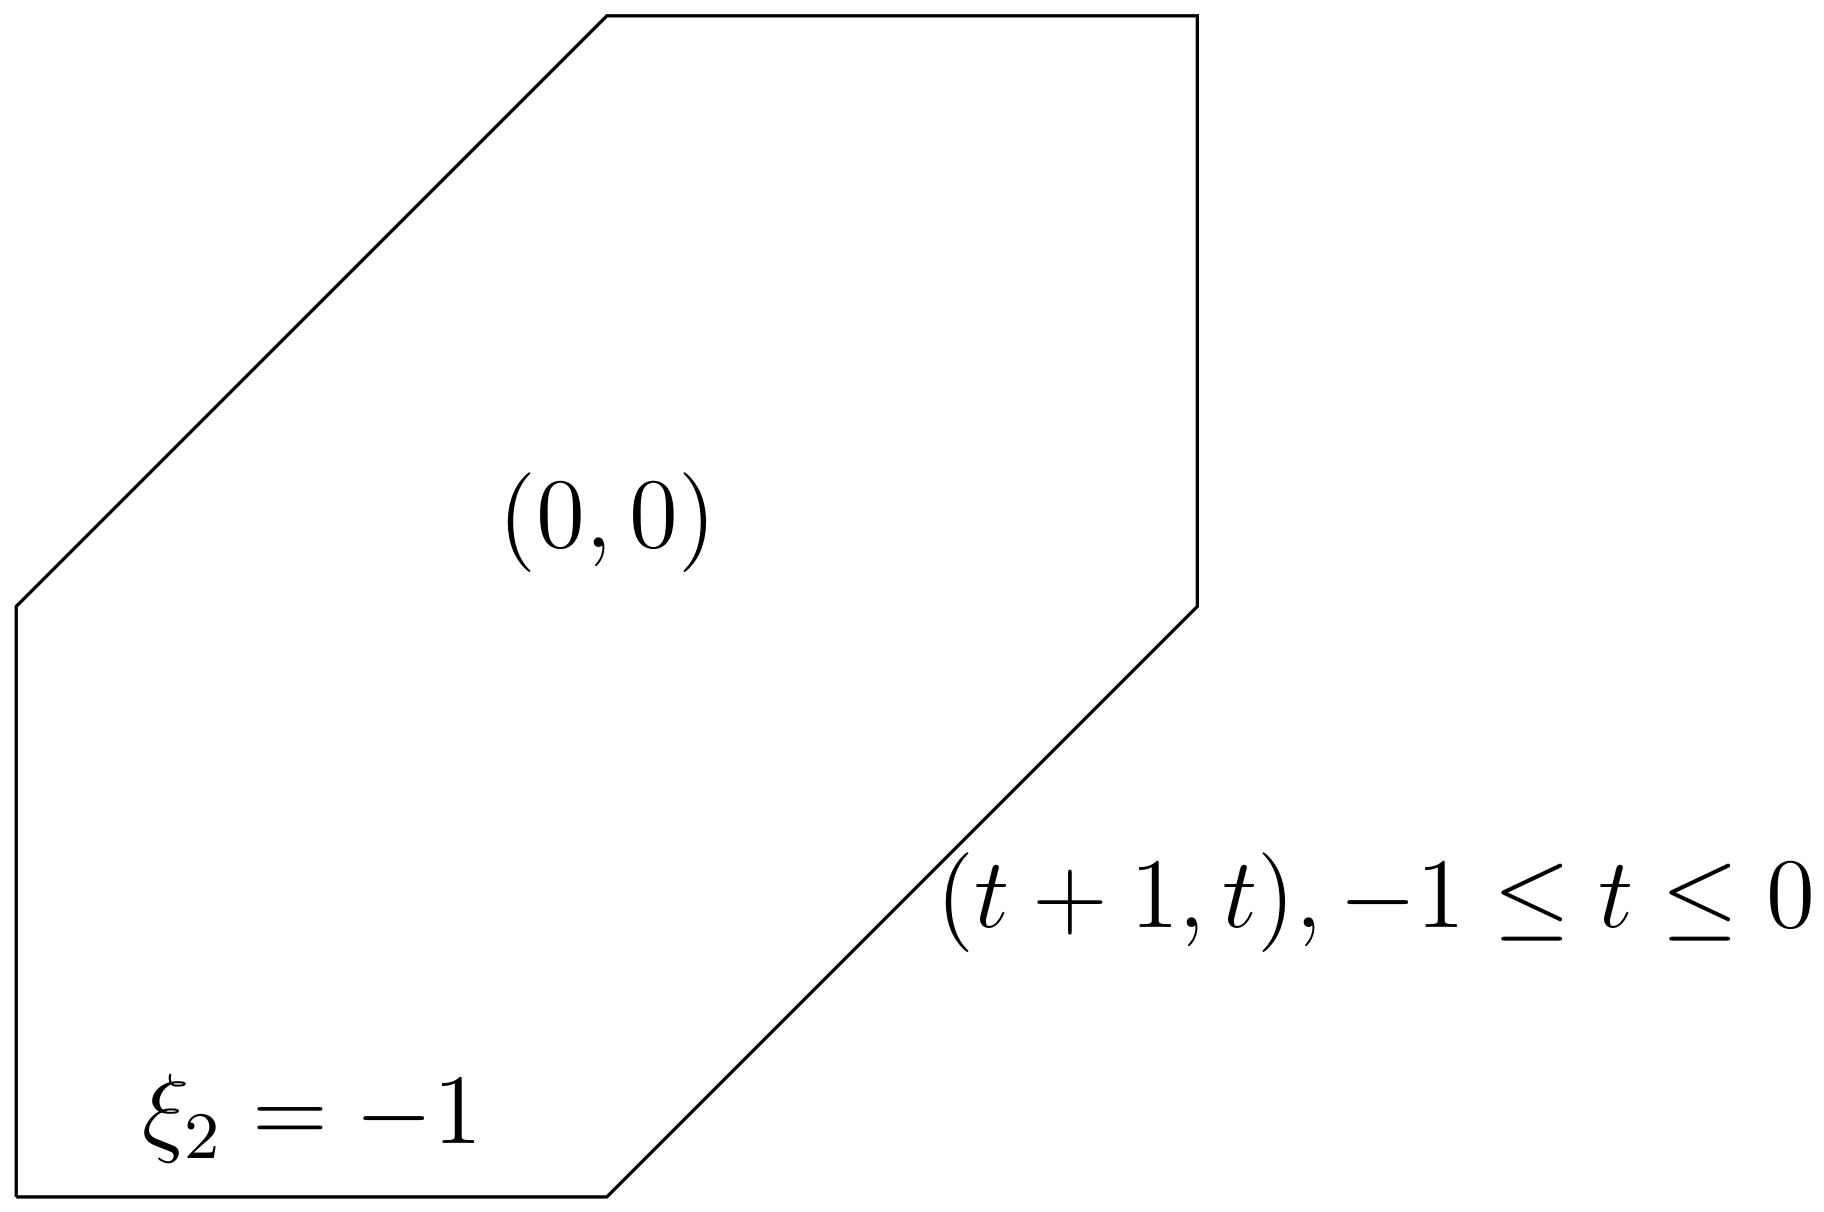
\includegraphics[width=0.52\textwidth]{figures/fig_1_2.png}
  \caption{由热带曲线界定的 $(0,0)$ 瓦片。（原书 p.26）}
  \label{fig:1-2}
\end{figure}

由周期性，这幅图铺满平面；由式~\eqref{eq:1-11}，$(m,n)$ 瓦片的斜率为
$m\xi_1+n\xi_2+\kappa(m\gamma'+n\gamma'')$。
\end{proof}

\transnote{证明只计算 $(0,0)$ 瓦片与相邻瓦片的交线；其余瓦片由 $\varphi$ 的周期性质（式~\eqref{eq:1-10}）平移得到。因此「蜂巢」是同一六边形沿 $\gamma'$、$\gamma''$ 两个方向铺成的。}

\medskip\noindent\textbf{概览：$(Y,v_0)$ 与 $\omega$ 的定义}\par

光滑流形 $Y$ 由环簇 $\tilde Y$ 的一部分取商得到；$\Gamma_B$ 通过全纯映射真不连续地作用。
其定义多面体为
\begin{equation}\label{eq:1-12}
\begin{gathered}
\Delta_{\tilde Y}:=\{(\xi_1,\xi_2,\eta)\in\R^3
  \mid\eta\ge\operatorname{Trop}(s)(\xi)\}\\
\Delta_Y:=(\Delta_{\tilde Y})|_{\eta\le T^l}/\Gamma_B\quad\text{其中}\\
\gamma\cdot(\xi_1,\xi_2,\eta):=(\xi_1+\gamma_1,\xi_2+\gamma_2,
  \eta-\kappa(\gamma)+\ip{\xi}{\lambda(\gamma)})\\
\because\operatorname{Trop}(s)(\xi+\gamma)=\operatorname{Trop}(s)(\xi)
  -\kappa(\gamma)+\ip{\xi}{\lambda(\gamma)}.
\end{gathered}
\end{equation}

多面体 $\Delta_{\tilde Y}$ 见图~\ref{fig:1-7}：$\eta$ 的下界由瓦片中央的表达式给出，
方向朝纸面外。复坐标将在下文讨论；此处先给出定义。

\transnote{作用 $\gamma\cdot$ 在 $(\xi_1,\xi_2)$ 方向平移，在 $\eta$ 方向平移并剪切，
恰好抵消 $\operatorname{Trop}(s)$ 在平移下的变化，所以图像在商下保持不变。这正是
$\Delta_Y$ 能良定义的原因。}

% ===== 原书 p.27 =====
\begin{definition}[{[AAK16][Definition 1.2]}]\label{def:syz-mirror}
称 $(Y,v_0)$ 为 $H=\Sigma_2$ 的广义 SYZ 镜像（generalized SYZ mirror）。
\end{definition}

\begin{remark}\label{rem:reverse-syz}
注意可以反向使用 SYZ：从 $Y$ 挖去一个除子后剩下的拉格朗日环面丛出发，把 $X$ 恢复为其
复镜像；参看 [AAK16, §8] 或 [CLL12]。
\end{remark}

\medskip\noindent\textbf{pair of pants：局部模型}\par

我们给出广义 SYZ 的一个示例，它是本文设定的局部模型。

\begin{example}[{[AAK16][§9.1]}]\label{ex:pants}
设 $H\subset V$ 是 $V=(\C^*)^2$ 中的 pair of pants（三孔球面）
$f(x_1,x_2):=1+x_1+x_2=0$。称之为 pair of pants，是因为
$x_1\in\C^*\setminus\{-1\}$，而柱面去掉一点正是 pair of pants。回忆
定义~\ref{def:tropicalization} 中 $\operatorname{Trop}(f)$ 的定义。
\end{example}

于是在 pair of pants 一例中 $\rho\equiv0$、$A=\{(0,0),(1,0),(0,1)\}$，因此
$\operatorname{Trop}(f)(\xi_1,\xi_2)=\max\{0,\xi_1,\xi_2\}$。若 $\xi_1,\xi_2<0$，
最大值为 $0$；若 $\xi_1>\xi_2>0$，最大值为 $\xi_1$；若 $\xi_2>\xi_1>0$，最大值为
$\xi_2$。所以 $\operatorname{Trop}(f)$ 的零点集（定义~\ref{def:vanishing}）如下图：

\begin{figure}[htbp]
  \centering
  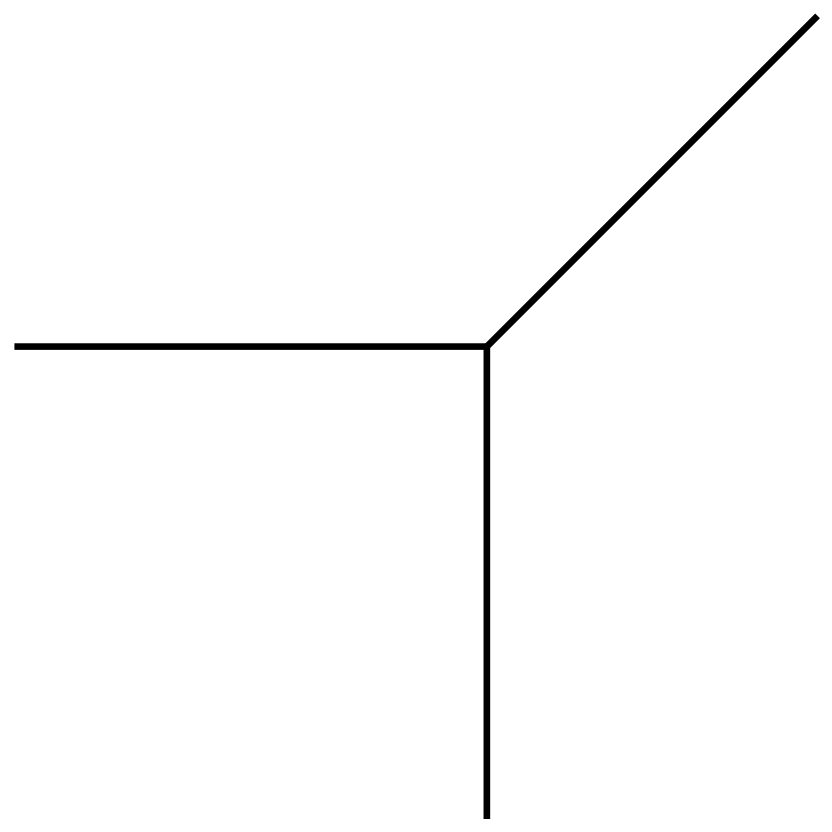
\includegraphics[width=0.2\textwidth]{figures/fig_1_3.png}
  \caption{$\operatorname{Trop}(1+x_1+x_2)=0$。（原书 p.27）}
  \label{fig:1-3}
\end{figure}

而矩多面体为 $\Delta:=\{(\xi,\eta)\mid\eta\ge\operatorname{Trop}(f)(\xi)\}
\subset\R^{n+1}$，如下图：

\begin{figure}[htbp]
  \centering
  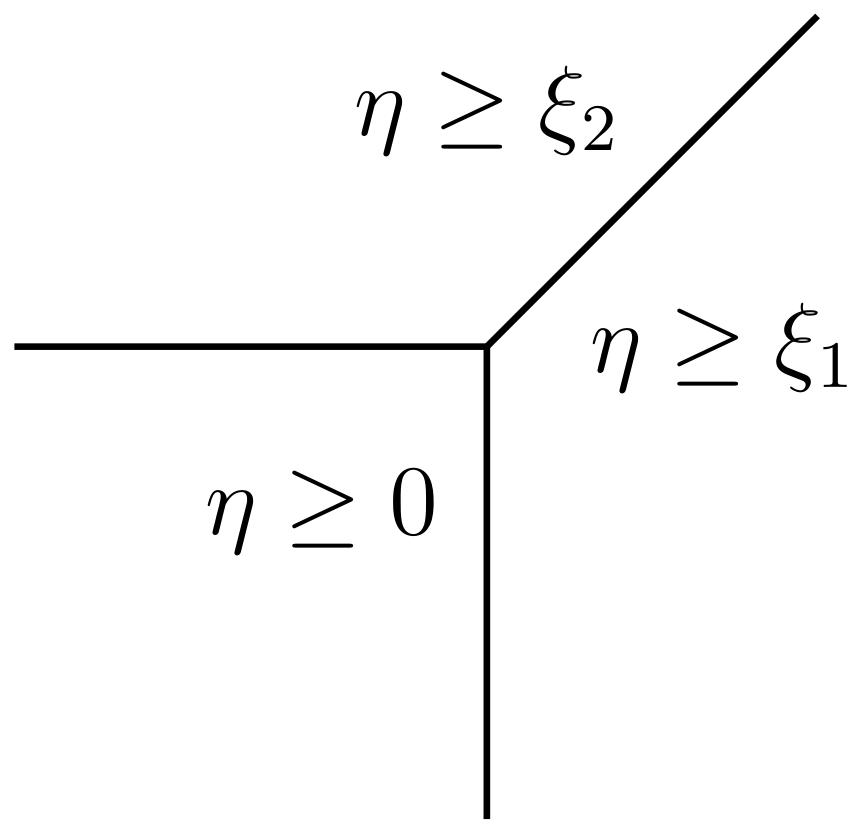
\includegraphics[width=0.26\textwidth]{figures/fig_1_4.png}
  \caption{矩多面体 $\subset\R^3$。（原书 p.27）}
  \label{fig:1-4}
\end{figure}

对 $(\xi_1,\xi_2,\eta)$ 作线性变换后，该多面体变为 $\R^3_{\ge0}$。相应的环簇是
$\operatorname{Spec}\C[x,y,z]=\C^3$。超势为 $v_0=xyz$，于是得到 pair of pants 的
预期镜像 $(\C^3,xyz)$。

\transnote{三点爆破的 $\C\PP^2$ 与 pair of pants 是同一局部模型的两种外观：前者是矩
多面体（六边形），后者是超曲面 $1+x_1+x_2=0$。多面体的每个顶点对应一个 $\C^3$
坐标卡，这正是后文用 $g_{xy}$ 在顶点附近插值的原因。}

% ===== 原书 p.28 =====
\medskip\noindent\textbf{$\omega$ 决定复坐标上的 $\Gamma_B$-作用}\par

我们要构造辛形式 $\omega$，使 1) 它是凯勒的，即与复环簇坐标继承的复结构相容；
2) $v_0:=xyz$ 是辛纤维丛；3) 它是环簇的，即在环面作用下不变。

由 3)，只需用复坐标的模长来定义辛形式。为保证 1)，局部地把 $\omega$ 写成某个凯勒势的
$\frac{i}{2\pi}\partial\bar\partial$，其中 $\partial\bar\partial$ 针对局部复环簇坐标。
为保证 2)，辛形式限制到每个纤维上都应是辛的。中心纤维是矩多面体由图~\ref{fig:1-5}
中六边形给出的环簇，再对 $\Gamma_B$ 取商。按 §1.3 的理论，它连同环簇
$\C\PP^2(3\text{ points})$（三点爆破）自带一个辛形式。离开 $v_0=0$ 但仍靠近多面体顶点
时，环簇局部地以例~\ref{ex:pants} 的局部模型 $(\C^3,xyz)$ 为模型。因此我们将用鼓包函数，
在 $\C\PP^2(3\text{ points})$ 的环簇辛形式与 $\C^3$ 上的标准形式之间插值。

\begin{figure}[htbp]
  \centering
  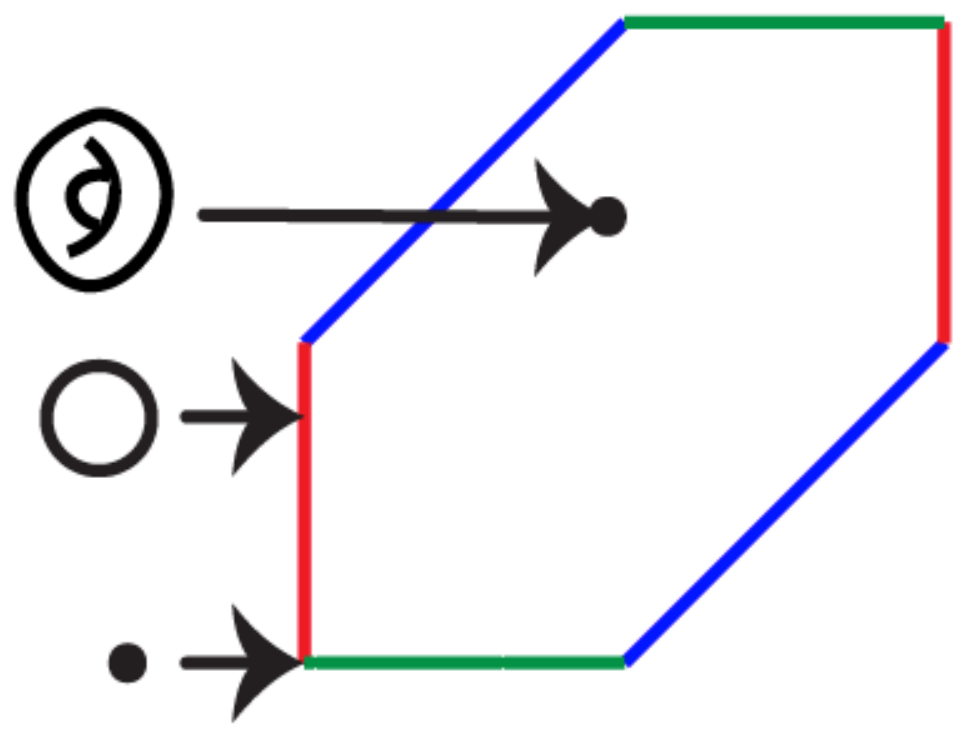
\includegraphics[width=0.28\textwidth]{figures/fig_1_5.png}
  \caption{$H=\Sigma_2$ 时 $(Y,v_0)$ 中心纤维的矩多面体。（原书 p.28）}
  \label{fig:1-5}
\end{figure}

下面解释降一维情形下辛形式构造的图示动机。

\begin{example}\label{ex:lower-dim}
设 $H$ 是椭圆曲线内的一点。此时多面体 $\Delta_{\tilde Y}$ 是二维的，可以画出来。
\end{example}

$v_0\colon\tilde Y\to\C$ 的纤维拓扑上是柱面；当 $|v_0|\to0$ 时，颈部周期性地被掐细，
退化为中心纤维上方的一串 $\PP^1$。在柱面最宽处，它看起来像球面的一部分，而 $\PP^1$
典范地带有富比尼–施图迪形式（Fubini--Study form）。另一方面，多面体顶点的邻域给出
坐标卡 $\C^2$，即 Lefschetz 纤维丛 $\C^2\to\C$、$(x,y)\mapsto xy$ 的局部图像，其中
柱面退化为以零点为顶点的锥。特别地，$\C^2$ 典范地带有标准形式 $\omega_{\mathrm{std}}$。
当环簇坐标很小时，由 $\log$ 的 Taylor 展开，富比尼–施图迪形式与标准形式近似相等。
因此在两个凯勒形式之间插值，即可构造辛形式。

% ===== 原书 p.29 =====
\begin{figure}[htbp]
  \centering
  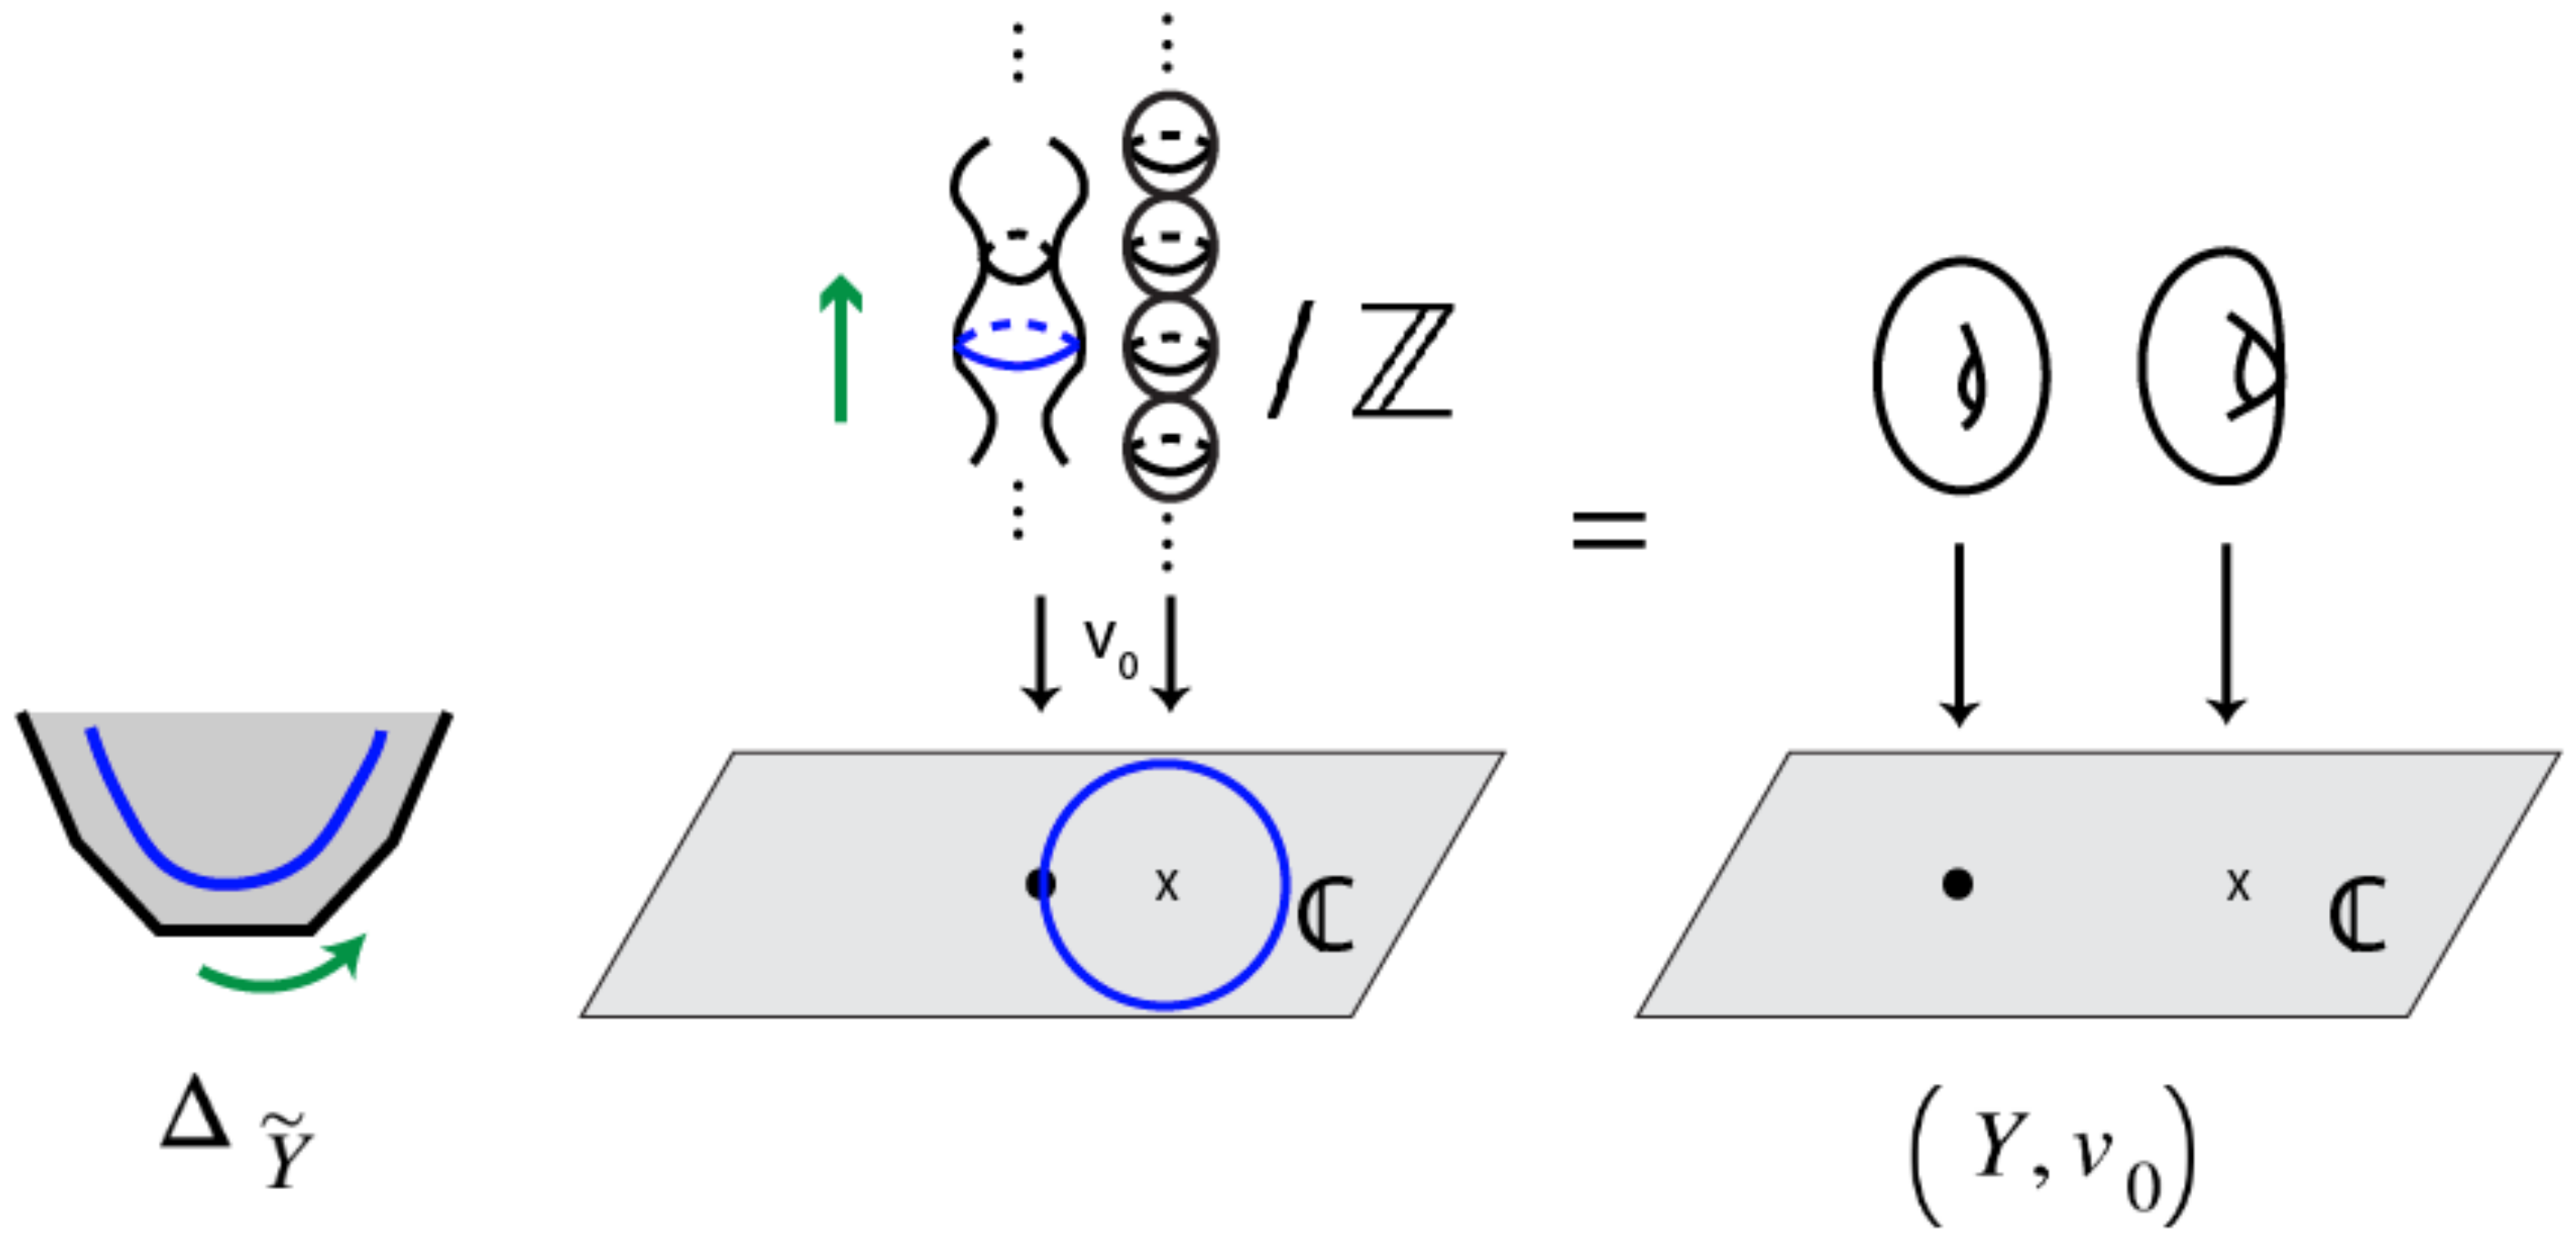
\includegraphics[width=0.8\textwidth]{figures/fig_1_6.png}
  \caption{降一维看，$\Delta_{\tilde Y}$ 的边界是一串 $\PP^1$ 的矩映射像。在多面体中
  $|v_0|$ 沿 $(0,1)$ 方向递增；在纤维丛 $v_0$ 中，$|v_0|$ 是底空间中圆的半径。
  （原书 p.29）}
  \label{fig:1-6}
\end{figure}

\begin{lemma}\label{lem:interpolation}
设 $r_x=|x|$，其余坐标同理，并设 $0<T\ll1$ 为常数。当 $H=\Sigma_2$ 时，
辛形式会在两种形式之间插值：一是顶点附近的局部坐标卡给出的 $(\C^3,\omega_{\mathrm{std}})$，
其凯勒势为 $\frac13T^2(r_x^2+r_y^2+r_z^2)$；
二是由六边形作为 $\C\PP^2$ 的三点爆破所诱导的环簇凯勒形式。
该凯勒势是「适当缩放的、对应格点的截面的平方和」的对数，如原书 1.3.29 的推论所述。
\end{lemma}

对某个 $(a,b,c)$，置
$g_{xy}:=\log(1+|T^ax|^2)(1+|T^by|^2)(1+|T^cxy|^2)$。
则 $(a,b,c)=(1,1,2)$ 具有正确的对称性，
使 $\omega$ 与 $\Gamma_B$-作用相容，并在商 $\tilde Y/\Gamma_B$ 上定义辛形式。

\transnote{引理中的「插值」有两层：一是在 $(\C^3,\omega_{\mathrm{std}})$ 与 $\C\PP^2$ 三点爆破的环簇形式之间插值；二是 $g_{xy}$ 中指数 $(a,b,c)$ 的选取要满足 $\Z/6$ 与 $\Gamma_B$ 的对称性。后文把这两层分别落实为鼓包函数与 $(a,b,c)=(1,1,2)$。}

\begin{remark}\label{rem:gxy-approx}
当 $Tr_x$ 与 $Tr_y$ 都很小时，有 $g_{xy}\approx(Tr_x)^2+(Tr_y)^2$。
\end{remark}

\begin{remark}\label{rem:figure17-scaling}
考察图~\ref{fig:1-7}，它画出本文的三维 $\Delta_{\tilde Y}$。
由环簇几何可知，$(x,y)$ 必定映到 $(y^{-1},xy)$ 的某个缩放，如图所示。
下文将定义合适的 $(\alpha,\beta)$，使该缩放为 $(x,y)\mapsto(T^\alpha y^{-1},T^\beta xy)$。
\end{remark}

\begin{definition}\label{def:G-action}
定义 $G=\Z/6\curvearrowright\tilde Y$，使六边形按如下方式顺时针旋转，
其中 $g$ 是 $G$ 的生成元：
\begin{equation}\label{eq:1-13}
g\cdot(x,y)=(T^\alpha y^{-1},T^\beta xy).
\end{equation}
更具体地说，$(x,y)$ 上的这一作用，通过指定它在 $v_0$ 的纤维上的限制，
决定了 $\tilde Y$ 上的作用；该纤维取一般纤维或退化的中心纤维。
换言之，$z$ 坐标上的作用是 $g\cdot z=T^{-\alpha-\beta}yz$，于是
$v_0=xyz\mapsto T^{\alpha+\beta-\alpha-\beta}y^{-1}\cdot xy\cdot yz=xyz$ 保持不变。
\end{definition}

\transnote{$\Z/6$-作用 $g$ 把六边形顺时针旋转一格；$\Gamma_B$ 则是由 $\gamma'$、$\gamma''$ 生成的平移群。两者在复坐标上的公式只差坐标置换 $\sigma_{g^n}$，务必分清「旋转」与「平移」两种操作。}

% ===== 原书 p.30 =====
\begin{figure}[htbp]
  \centering
  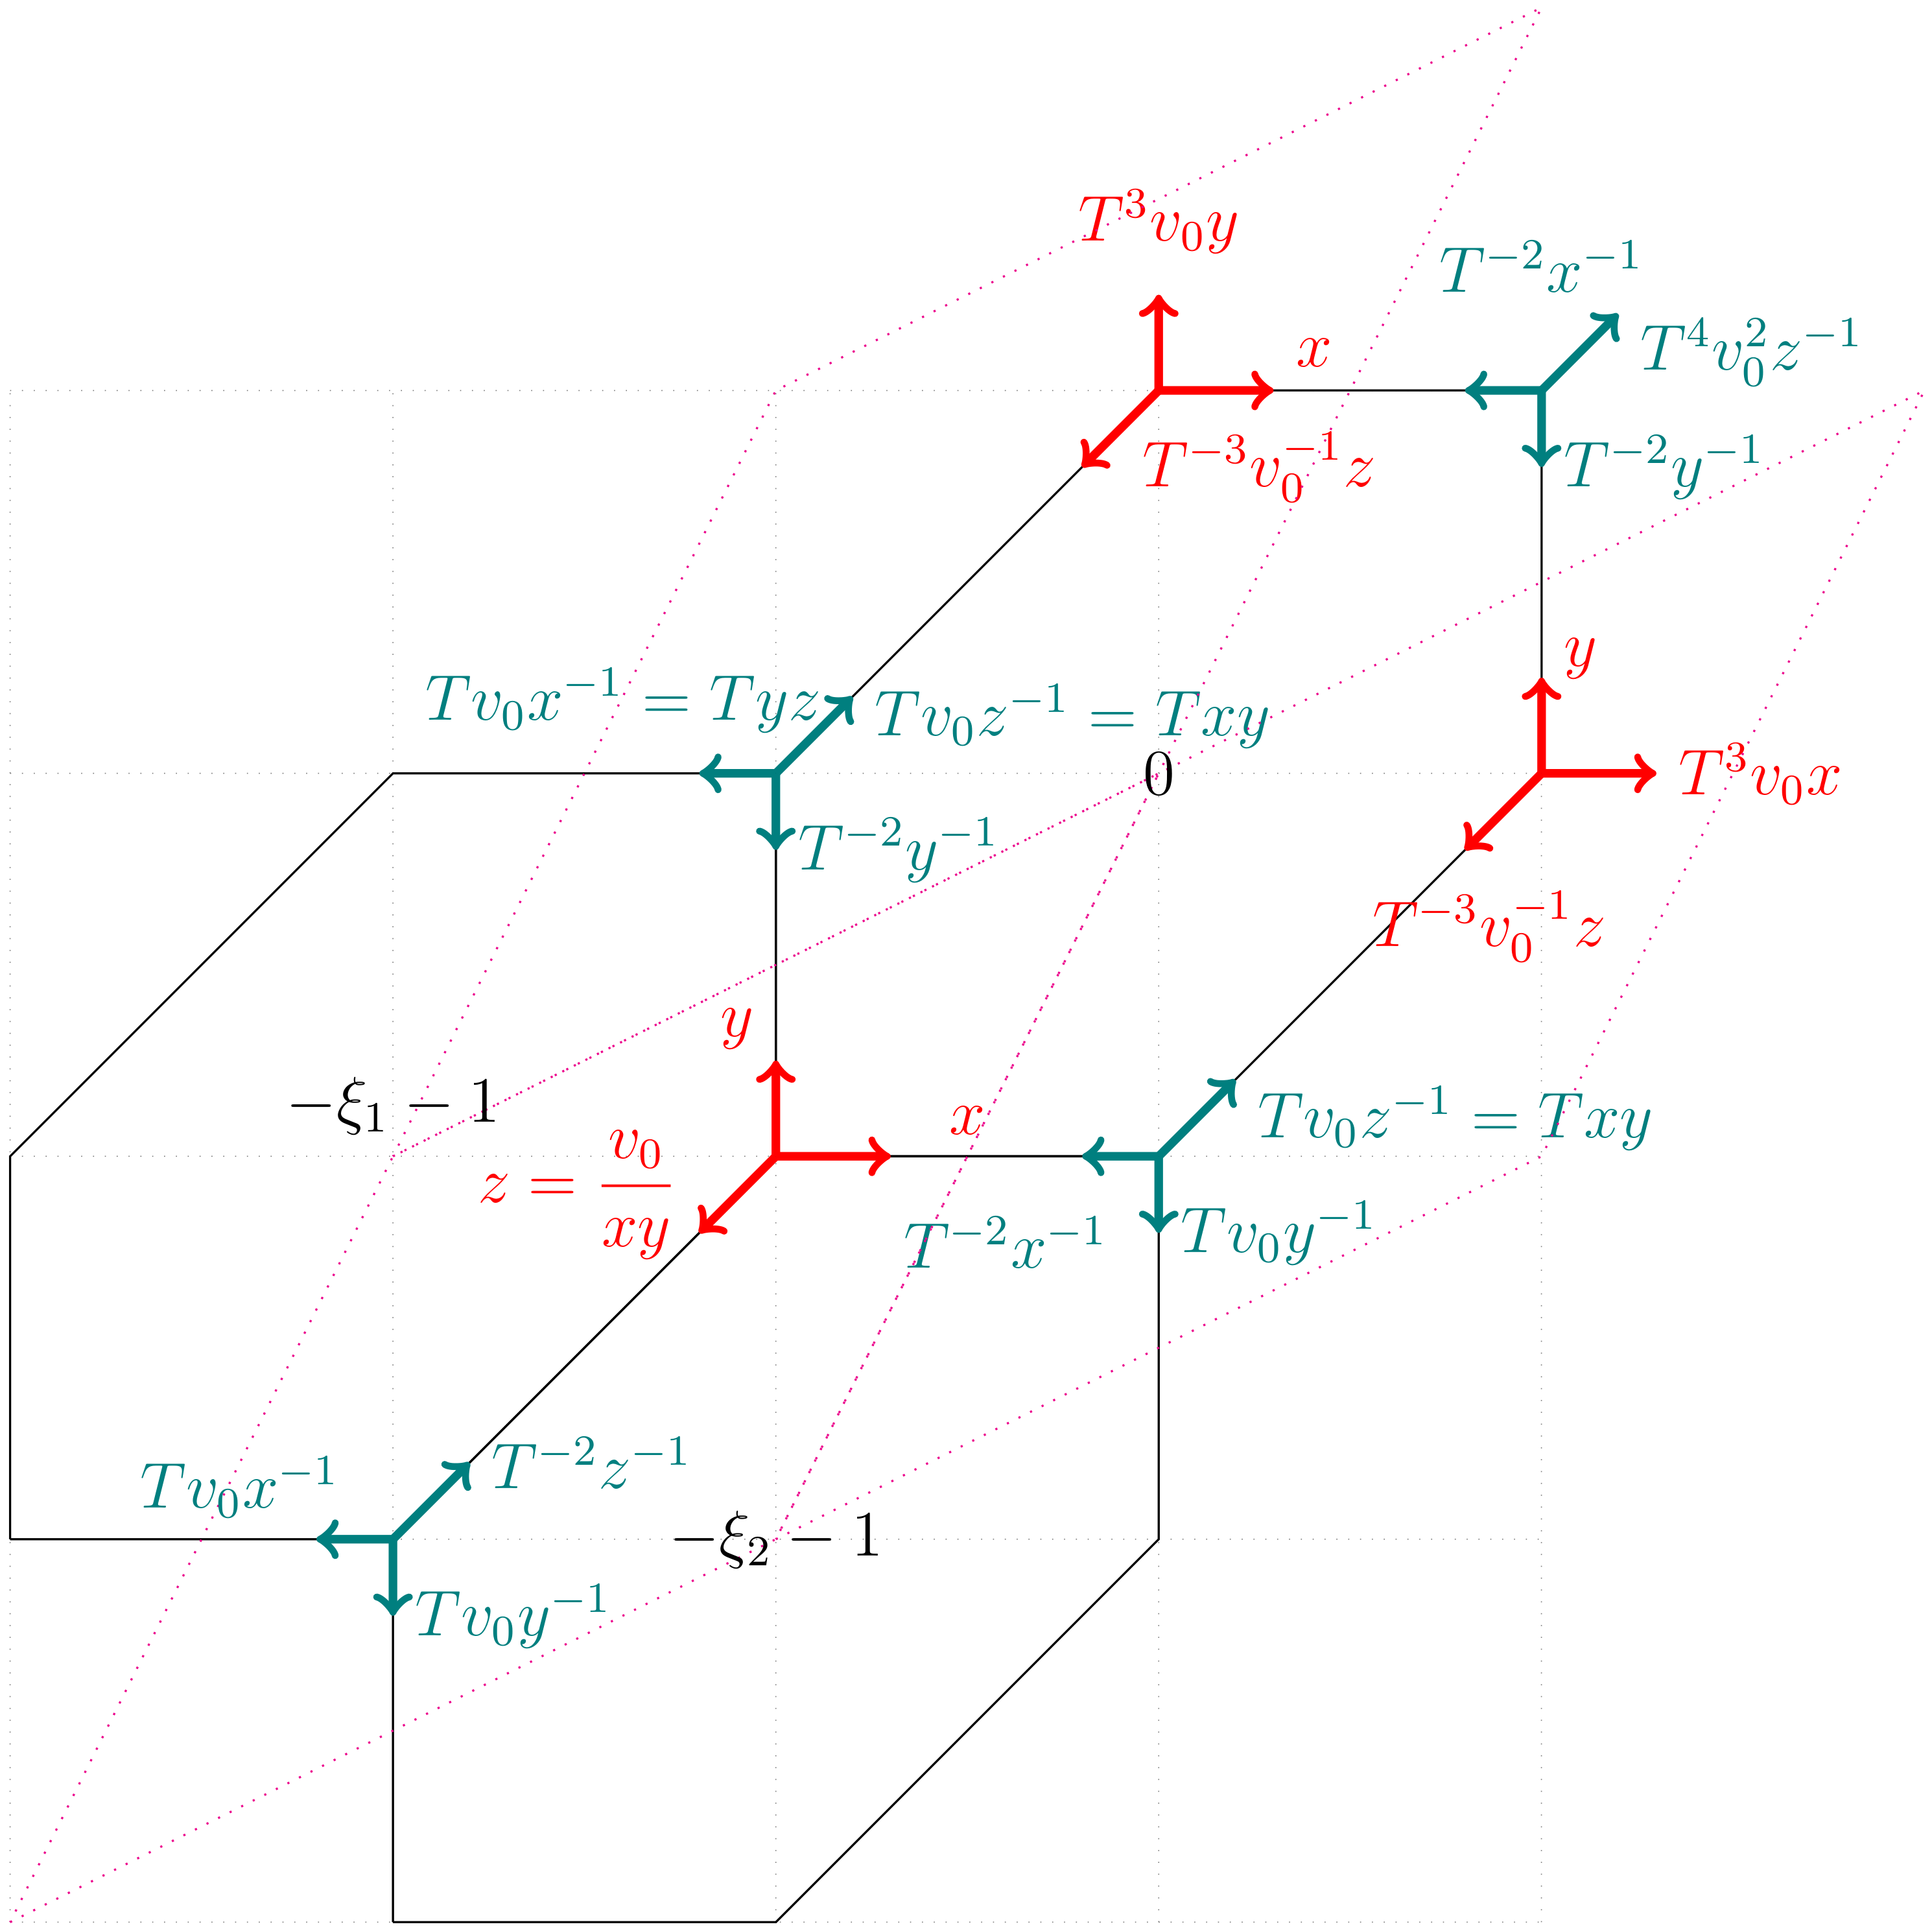
\includegraphics[width=0.8\textwidth]{figures/fig_1_7.png}
  \caption{$\Sigma_2$ 情形下 $\Delta_{\tilde Y}$ 的图示。图中坐标提示了
  $\Gamma_B$-作用，其动机与定义见后续各节。洋红色平行四边形是
  $\Gamma_B$-作用的基本域，中心为对角的 $\PP^1$。每个顶点是一个 $\C^3$ 坐标卡，
  坐标过渡将在引理~\ref{lem:interpolation} 中说明。瓦片中心处的表达式表示该瓦片上的
  $\eta\ge\varphi(\xi)=-\xi_1-1$ 一类不等式；六条边的方程表明瓦片 $(0,0)$ 由
  $(\xi_1,\xi_2)\in\{(\xi_1,\xi_2)\mid-1\le\xi_1,\xi_2,-\xi_1+\xi_2\le1\}$ 给出。
  （原书 p.30）}
  \label{fig:1-7}
\end{figure}

\begin{claim}\label{clm:area-one}
在 $G$ 作用下，若 $g_{xy}$ 映到的凯勒势只相差一个调和函数，
即相差 $\log|T^{\alpha/2}y|^2$，则沿 $y$ 轴的 $\PP^1$ 的辛面积为 $1$。
\end{claim}

\begin{proof}
我们沿 $z$ 轴计算。由对称性，沿 $y$ 轴的计算与之类似，故只需考虑前者。
注意由 Stokes 定理，沿 $z$ 轴的 $\PP^1$ 辛面积为 $1$。
回忆 $\PP^1$ 有开覆盖 $U_0,U_\infty$，坐标卡 $\varphi_0$ 与 $\varphi_1$
分别把 $[z_0:z_1]$ 送到 $z_1/z_0$ 与 $z_0/z_1$。
我们要把 $\PP^1$ 上的积分拆到这两个卡上，但只取到两卡相交之处，否则积分区域过大。
于是 $z$ 是 $\varphi_0(U_0)\cong\C$ 上的坐标，
% [Tutor Note: 原文此处称坐标卡为 φ1，而下式与后文均写作 φ∞；疑为同一张卡的笔误，保留原样。]

% ===== 原书 p.31 =====
它在 $\varphi_\infty(U_\infty)$ 上是 $1/(T^\alpha z)$，并且
$|z|=|1/T^\alpha z|\Longrightarrow|z|=1/T^{\alpha/2}$。
令 $D_0$ 为 $\varphi_0(U_0)$ 中的圆盘，$D_\infty$ 为另一卡中对应的圆盘。
设 $F_0,F_\infty$ 为两卡中的凯勒势。
\begin{align*}
\int_{\PP^1}\frac{i}{2\pi}\partial\bar\partial F
&=\frac{i}{2\pi}\Bigl[\int_{\varphi_0^{-1}(D_0)}d(\bar\partial F)
 +\int_{-\varphi_\infty^{-1}(D_\infty)}d(\bar\partial F)\Bigr]\\
&=\frac{i}{2\pi}\Bigl[\int_{\partial D_0}\bar\partial(\varphi_0^{-1})^*F
 -\int_{\partial D_\infty}\bar\partial(\varphi_\infty^{-1})^*F\Bigr]\\
&=\frac{i}{2\pi}\int_{C_{1/T^{\alpha/2}}}\bar\partial(F_0-F_\infty)\\
&=\frac{i}{2\pi}\int_{C_{1/T^{\alpha/2}}}\bar\partial\log(|T^{\alpha/2}z|^2)
 =\frac{i}{2\pi}\int_{C_{1/T^{\alpha/2}}}\frac{T^\alpha z\,d\bar z}{|T^{\alpha/2}z|^2}\\
&=\frac{i}{2\pi}\int_0^{2\pi}e^{i\theta}(-i)e^{-i\theta}\,d\theta=1.
\end{align*}
\end{proof}

\transnote{只需沿 $z$ 轴计算，其余两轴由 $(x,y,z)$ 的轮换对称性得到。积分拆到 $U_0$ 与 $U_\infty$ 两张卡，交线是圆 $C_{1/T^{\alpha/2}}$；最后一步为 $\int_0^{2\pi}e^{i\theta}(-i)e^{-i\theta}\,d\theta=2\pi$，再乘 $i/2\pi$ 得 $1$。}

\begin{proof}[{主引理~\ref{lem:interpolation} 的证明}]
\begin{gather*}
g^*\log(1+|T^ax|^2)(1+|T^by|^2)(1+|T^cxy|^2)\\
=\log(1+|T^{a+\alpha}y^{-1}|^2)(1+|T^{b+\beta}xy|^2)(1+|T^{c+\alpha+\beta}x|^2),\\
g_{xy}=\log(1+|T^ax|^2)(1+|T^by|^2)(1+|T^cxy|^2).
\end{gather*}
我们预期两个势相差 $\log|T^by|^2$，因为 $y$ 在 $g$ 下变为 $y^{-1}$。
比较指数得
\begin{gather*}
b=-a-\alpha,\\
a=c+\alpha+\beta,\\
c=b+\beta.
\end{gather*}
这里有 5 个未知量与 3 个方程，故应能化为 2 个未知量。
具体地，把 $(a,b,c)$ 用 $(\alpha,\beta)$ 表示，再要求 $x\leftrightarrow y$ 对称，
即令 $a=b$，从而用 $\beta$ 确定 $\alpha$。
\begin{align*}
a&=c+\alpha+\beta=(b+\beta)+\alpha+\beta=(-a-\alpha)+\alpha+2\beta\\
\Longrightarrow a&=\beta\\
\Longrightarrow b&=-\alpha-\beta\\
a=b\ \therefore\ \alpha&=-2\beta\\
\Longrightarrow c&=b+\beta=2\beta\\
\therefore\ g_{xy}&=\log(1+|T^\beta x|^2)(1+|T^\beta y|^2)(1+|T^{2\beta}xy|^2).
\end{align*}
取 $\beta=1$ $\Longrightarrow$ $g_{xy}=\log(1+|Tx|^2)(1+|Ty|^2)(1+|T^2xy|^2)$。

% ===== 原书 p.32 =====
由于取 $\beta=1$，可见沿 $x$ 轴（由对称性，沿 $y$、$z$ 轴亦然）复坐标的模改变 $T^{-2}$。
于是施加 $g$ 时 $y$ 的值变大；但那里新的坐标系（后文记作 $(x'',y'',z'')$）
与原 $(x,y,z)$ 处一样取小值。
\end{proof}

\transnote{「$y$ 的值变大」说的是旧坐标在新卡中的量级，相差 $T^{-2}$；
换到新卡 $(x'',y'',z'')$ 后各坐标仍取小值。读图~\ref{fig:1-7} 时不宜把两者混为一谈。}

下一节将说明为何 $(\alpha,\beta)=(-2,1)$ 与 $g\cdot(x,y)=(T^{-2}y^{-1},Txy)$
给出图~\ref{fig:1-7} 所画的 $\Gamma_B$-作用。
由此便可定义 $Y$ 为商 $\tilde Y/\Gamma_B$；
其中 $\tilde Y$ 由 $\Delta_{\tilde Y}$ 按 §1.3 所述构造。

\medskip\noindent\textbf{$Y$ 的定义}\par

\begin{remark}[约定]\label{rem:convention}
约定：在图~\ref{fig:1-7} 中向上、向右移动为负方向。
因为 $T\ll1$ 的正幂次使坐标值变小，而坐标值变小对应沿群作用的负方向移动。
也就是说，$\gamma'$ 与 $\gamma''$ 的作用分别把坐标 $(x,y,z)$ 送到
图~\ref{fig:1-7} 中以 $(-2,-1)$ 与 $(-1,-2)$ 为中心的卡。
\end{remark}

\transnote{图~\ref{fig:1-7} 中坐标的指向与 $T$ 的幂次相反：$T\ll1$ 时 $T$ 的正幂次让坐标值变小，所以图上「向上、向右」对应群作用的负方向。核对 $\gamma'$、$\gamma''$ 的像之前，先确认这一约定。}

\begin{definition}[$\Gamma_B$-作用的定义]\label{def:GammaB-action}
$(x,y,z)$ 上的 $\Gamma_B$-作用可由定义~\ref{def:G-action} 中定义的 $\Z/6$-作用读出。
即 $g^2$ 像 $-\gamma''$ 那样，把 $(x,y,z)$ 送到以 $(\xi_1,\xi_2)=(1,2)$ 为中心的坐标系；
但它是通过旋转来置换坐标方向的。
事实上，$g$ 把 $(x,y,z)\mapsto(T^{-2}y^{-1},Txy,Tyz)$。
为抵消 $g$ 中的这一置换、使方向保持不变，即
$(x,y,z)\mapsto(Tyz,T^{-2}y^{-1},Txy)=(Tv_0x^{-1},T^{-2}y^{-1},Tv_0z^{-1})$；
对施加 $g^2$ 所得的坐标作同样的置换，即可定义 $\Gamma_B$-作用：
\[
(-\gamma'')\cdot(x,y,z):=(x,T^3v_0y,T^{-3}v_0^{-1}z).
\]
\end{definition}

\begin{definition}[{$Y$ 的定义}]\label{def:Y}
现在可以用商 $\tilde Y/\Gamma_B$ 定义 $Y$：
\begin{equation}\label{eq:1-14}
\begin{gathered}
\Delta_{\tilde Y}:=\{(\xi_1,\xi_2,\eta)\in\R^3\mid\eta\ge\operatorname{Trop}(s)(\xi)\}\\
\Delta_Y:=(\Delta_{\tilde Y})|_{\eta\le T^l}/\Gamma_B\quad\text{其中式~\eqref{eq:1-10} 表明}\\
\gamma\cdot(\xi_1,\xi_2,\eta):=(\xi_1+\gamma_1,\xi_2+\gamma_2,\eta-\kappa(\gamma)+\ip{\xi}{\lambda(\gamma)}).
\end{gathered}
\end{equation}
\end{definition}

$\Delta_{\tilde Y}$ 的每个顶点对应三个复坐标，可以用 $(x,y,z)$（以及 $v_0=xyz$）写出。
图~\ref{fig:1-7} 列出了这些坐标；为清楚起见，我们在此把它们收集为坐标卡 $U_{n,g^k}$。
其中 $\gamma=n_1\gamma'+n_2\gamma''$ 表示所看瓦片在 $\Delta_{\tilde Y}$ 中投影到前两个坐标后的中心，
$g^k$ 表示绕六边形走到了何处。
$g^k$ 只用来索引坐标卡；但如定义~\ref{def:GammaB-action} 所述，
坐标是 $g^k\cdot(x,y,z)$ 的置换，所以下标主要用于索引。过渡映射为
\[
(x,y,z)\mapsto\sigma_{g^n}\cdot(g^n\circ\gamma)\cdot(x,y,z),
\qquad n\in\Z/6,\ \gamma\in\Gamma_B.
\]

% ===== 原书 p.33 =====
其中 $\sigma_{g^n}$ 是坐标的某个置换，依赖于 $n$，见定义~\ref{def:GammaB-action}。
从 $(x,y,z)$ 出发，沿 $(0,0)$ 瓦片顺时针走：
\begin{itemize}[leftmargin=2.2em,itemsep=0.25em]
\item $U_{0,g^0}$：$(x,y,z)$。
\item $U_{0,g}$：$(Tv_0x^{-1},T^{-2}y^{-1},Tv_0z^{-1})=:(x'',y'',z'')$。
\item $U_{0,g^2}$：$(x,T^3v_0y,T^{-3}v_0^{-1}z)=:(-\gamma'')\cdot(x,y,z)$。
\item $U_{0,g^3}$：$(T^{-2}x^{-1},T^{-2}y^{-1},T^4v_0^2z^{-1})$。
\item $U_{0,g^4}$：$(T^3v_0x,y,T^{-3}v_0^{-1}z)=:(-\gamma')\cdot(x,y,z)$。
\item $U_{0,g^5}$：$(T^{-2}x^{-1},Tv_0y^{-1},Tv_0z^{-1})=:(x',y',z')$。
\item 沿 $z$ 轴走，可到 $(-1,0)$ 瓦片中的 $g^{-1}$ 顶点：
\item $U_{(-1,0),g^{-1}}$：$(Tv_0x^{-1},Tv_0y^{-1},T^{-2}z^{-1})=:(x''',y''',z''')$。
\end{itemize}

于是：当 $|v_0|=T^l$、$T\ll1$ 且 $l$ 充分小时，$\Gamma_B$ 真不连续地全纯作用，
故商是良定义的复流形 $Y$。
% [Tutor Note: 原文作「l sufficiently small」；但要使 |v0|=T^l 很小（T<<1），应需 l 充分大。保留原样，登记为疑点。]

\begin{proof}[{由 $\Z/6$-作用计算坐标}]
由于 $g\cdot(x,y)=(T^{-2}y^{-1},Txy)$，把群作用施加两次得
\[
(x,y)\sim(T^{-2}y^{-1},Txy)\sim
\bigl(T^{-2}(T^{-1}x^{-1}y^{-1}),T(T^{-2}T^{-1})(Txy)\bigr)
=(T^{-3}x^{-1}y^{-1},x).
\]
% [Tutor Note: 原件第二分量写作 T(T^{-2}T^{-1})(Txy)，代入得 T^{-1}xy，与右侧的 x 不符；疑应为 T(T^{-2}y^{-1})(Txy)=x。保留原样，登记为疑点。]
特别地，$\Gamma_B$ 固定 $v_0=xyz$，故可把变换后的 $y$ 坐标改写为 $T^3v_0y$，
从而在适当的置换 $\sigma_{g^2}$ 之后得到 $\gamma''$-作用：
\[
\sigma_{g^2}\cdot g^2\cdot(x,y,z)=:-\gamma''\cdot(x,y,z)
=(x,T^3v_0y,T^{-3}v_0^{-1}z).
\]
$\gamma'$ 的计算与之类似。为求坐标系 $(x''',y''',z''')$，
先沿 $\gamma'$ 的作用向左下方移动，进入 $(0,-1)$ 瓦片，
再用 $g^{-1}$ 旋转，最后施加适当的置换。
由于 $g^{-1}\cdot(x,y)=(Txy,T^{-2}x^{-1})$，得
$g^{-1}\cdot(x,y,z)=(Tv_0z^{-1},T^{-2}x^{-1},Tv_0y^{-1})$。于是
\begin{align*}
\gamma'\cdot(x,y,z)&=(T^{-3}v_0^{-1}x,y,T^3v_0z),\\
g^{-1}\cdot(T^{-3}v_0^{-1}x,y,T^3v_0z)
&=\bigl(Tv_0(T^3v_0z)^{-1},T^{-2}(T^{-3}v_0^{-1}x)^{-1},Tv_0y^{-1}\bigr)\\
&=(T^{-2}z^{-1},Tv_0x^{-1},Tv_0y^{-1}),\\
\therefore\ (x''',y''',z''')
&:=\sigma_{g^{-1}}\cdot g^{-1}\cdot\gamma'\cdot(x,y,z)\\
&=(Tv_0x^{-1},Tv_0y^{-1},T^{-2}z^{-1}).
\end{align*}
\end{proof}

上面所列各卡中其余坐标的计算与此类似。

% ===== 原书 p.34 =====
\begin{remark}\label{rem:symmetry-told-structure}
注意，$\omega$ 所需的对称性质告诉我们需要何种复结构（它给出乘积复结构）；
由镜像对称，这将对应 $X$ 的 A 模型上某个特定的辛形式。
我们在定义~\ref{def:Y} 的列表中，用新的带撇变量标记图~\ref{fig:1-7} 的部分绿色坐标卡坐标。
\end{remark}

\begin{corollary}[{$Y$ 上的复结构}]\label{cor:complex-structure}
复结构这样得到：先把多面体 $\Delta_{\tilde Y}$ 每个顶点的环簇卡，
通过把 $(x,y,z)$ 与各其他顶点的新坐标系粘合而等同起来。
然后按 $\Gamma_B$-作用取商；该作用缩放坐标而保持 $v_0=xyz$，
故商上 $v_0$ 的纤维是阿贝尔簇。用复坐标写出，$\Gamma_B$-作用为
\[
(x,y,z)\sim(T^3v_0x,y,T^{-3}v_0^{-1}z),\qquad
(x,y,z)\sim(x,T^3v_0y,T^{-3}v_0^{-1}z).
\]
\end{corollary}

\begin{remark}\label{rem:gluing-rescaling}
注意，在按 $\Gamma_B$-作用取商之前，把所有环簇卡粘好后纤维会是 $(\C^*)^2$。
复坐标中的 $\Gamma_B$-作用，对应从 $\Delta_{\tilde Y}$ 过渡到
$\Delta_Y=\Delta_{\tilde Y}/\Gamma_B$。
我们仍按多面体等同单项式来粘环簇卡，但允许在粘合复坐标时发生缩放。
（例如低一维：对 $\C^*\ni x\mapsto Tx$，把单位圆与半径 $T$ 的圆粘起来，得到环面。）
\end{remark}

\begin{remark}[术语]\label{rem:terminology}
环簇 $\tilde Y$ 被 [KL19] 称为「无穷型」（infinite-type）环簇，
因为它的面有无穷多个；那里环簇除子的邻域，
等同于我们限制到 $|v_0|$ 小（即 $\eta$ 小）的情形。
\end{remark}

\begin{definition}[超势]\label{def:superpotential}
超势 $v_0$ 是全纯函数 $Y\to\C$，定义为
\begin{equation}\label{eq:1-15}
v_0(x,y,z):=xyz,
\end{equation}
它在 $Y$ 上是良定义的全局函数，因为它在 $\Gamma_B$-作用下不变。
\end{definition}

\begin{remark}\label{rem:symplectic-fibration}
我们将在第 2 章为 $v_0$ 配上辛纤维丛结构，
再在 §4.1 为它配上深谷–Seidel 范畴。
\end{remark}

\begin{remark}\label{rem:AAK16-comparison}
这里的复坐标上的 $\Gamma_B$-作用与 [AAK16, §10.2] 所述不同。
这意味着 $Y$ 作为 $X$ 的镜像，所用的辛形式与其论文中的不同。那里的复结构是
\begin{equation}\label{eq:1-16}
\boldsymbol{v}^m\sim v_0^{\ip{\lambda(\gamma)}{m}}T^{\ip{\gamma}{m}}\boldsymbol{v}^m,
\end{equation}
其中用复坐标 $\boldsymbol{v}=(v_1,v_2)$。于是置 $(x,y,z)=(v_1^{-1},v_2^{-1},v_0v_1v_2)$，
其复结构来自如下 $\Gamma_B$-作用：
\begin{gather*}
\gamma'\cdot(x,y,z)=(T^{-2}v_0^{-1}x,T^{-1}y,T^3v_0z),\\
\gamma''\cdot(x,y,z)=(T^{-1}x,T^{-2}v_0^{-1}y,T^3v_0z).
\end{gather*}
\end{remark}

% ===== 原书 p.35 =====
\medskip\noindent\textbf{把多面体划分为区域}\par

回忆图~\ref{fig:1-7} 的多面体 $\Delta_{\tilde Y}$。
我们先在一个顶点的邻域内定义 $\omega$。
它用 $\tilde Y$ 上一组新的局部实径向与角向坐标 $d$ 与 $\theta$ 定义，
在图~\ref{fig:1-9} 的每个划分区域内各有一套。

这些划分由下列变量给出。固定 $|v_0|(=|xyz|)=T^l$，
其中 $T\ll1$，$l$ 是大的正常数。
在图~\ref{fig:1-9} 的支集内，$r_x,r_y,r_z\ll1$，
故式~\eqref{eq:1-18} 的近似成立。

定义函数 $\phi_x,\phi_y,\phi_z$，它们对理解后续计算至关重要。
\begin{equation}\label{eq:1-17}
\begin{gathered}
\phi_x(x,y,z):=\log_T\frac{1+|Tx|^2}{1+|T^2yz|^2},\\
\phi_y(x,y,z):=\log_T\frac{1+|Ty|^2}{1+|T^2xz|^2},\\
\phi_z(x,y,z):=\log_T\frac{1+|Tz|^2}{1+|T^2xy|^2}.
\end{gathered}
\end{equation}

现在可以定义计算中要用的局部径向与角向坐标。
它们的下标表示其定义所在的是图 1.4 的哪个区域。
% [Tutor Note: 此处划分区域画在图 1.8/1.9，原文「图 1.4」疑为「图 1.9」之误。保留原样，登记为疑点。]

\begin{figure}[htbp]
  \centering
  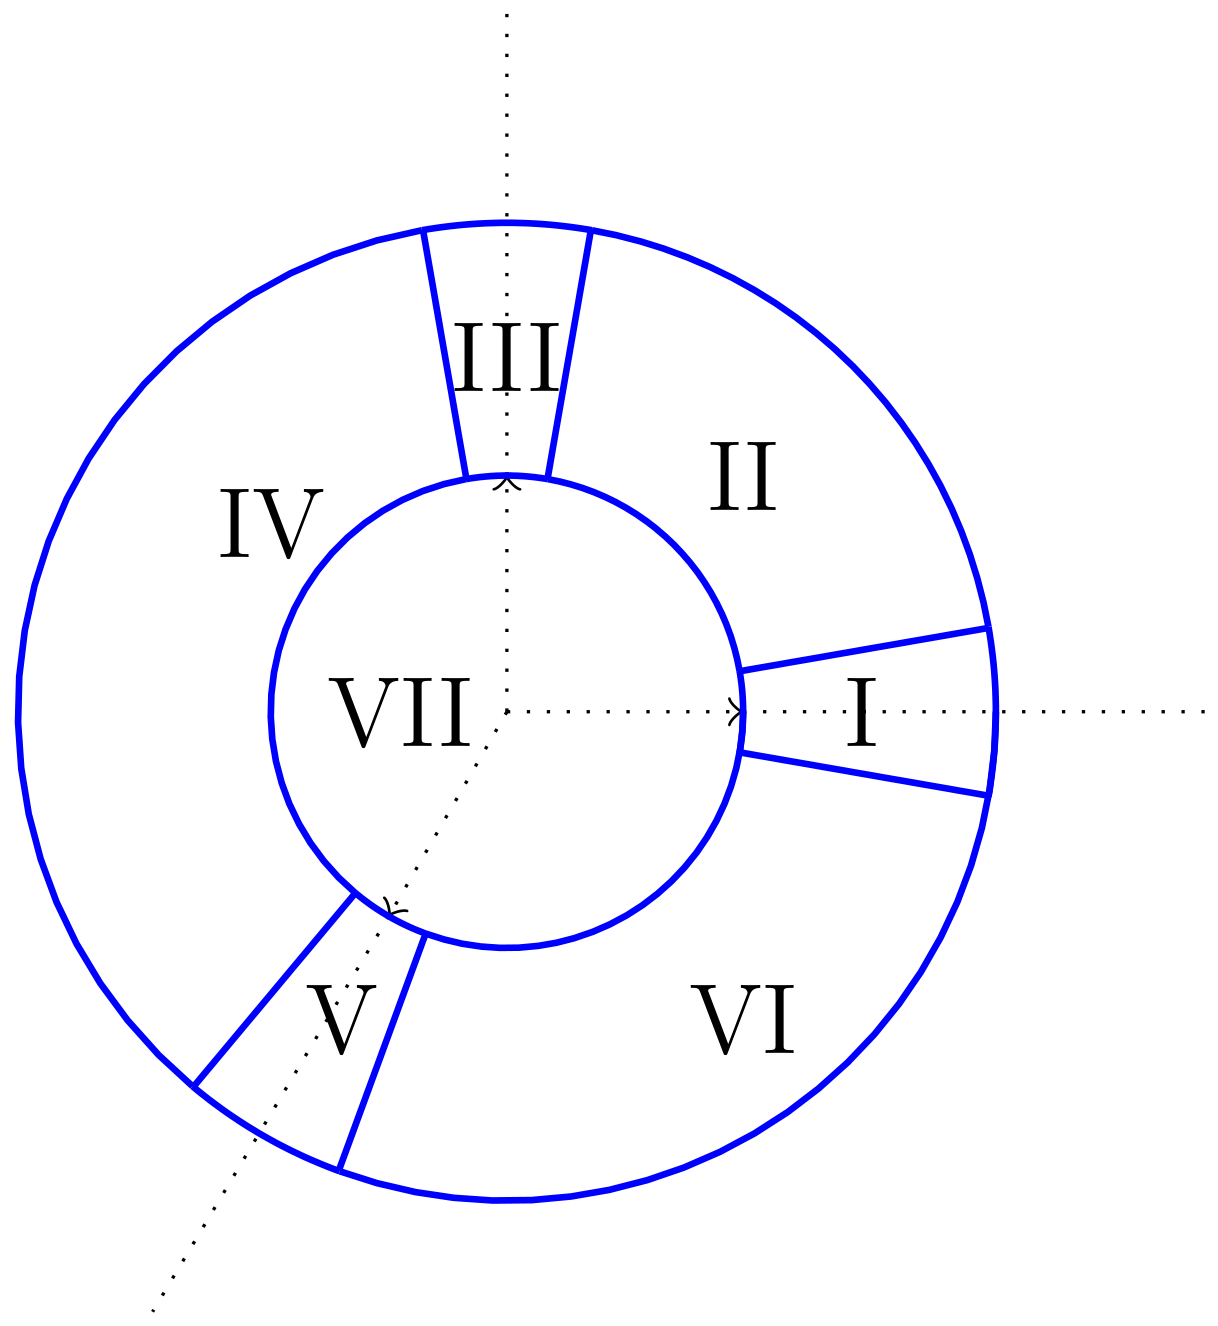
\includegraphics[width=0.3\textwidth]{figures/fig_1_8.png}
  \caption{围绕一个顶点划分 $\Delta_{\tilde Y}$ 中的区域。（原书 p.35）}
  \label{fig:1-8}
\end{figure}

% ===== 原书 p.36 =====
\begin{equation}\label{eq:1-18}
\begin{gathered}
d_I:=\phi_x-\frac12(\phi_y+\phi_z)\\
=\log_T\Biggl(\frac{1+|Tx|^2}{1+|T^2v_0x^{-1}|^2}\Bigg/
\sqrt{\frac{1+|Ty|^2}{1+|T^2v_0y^{-1}|^2}\cdot
\frac{1+|Tz|^2}{1+|T^2v_0z^{-1}|^2}}\Biggr)\\
\approx(Tr_x)^2-\frac12\bigl((Tr_y)^2+(Tr_z)^2\bigr)
\qquad\text{当 }r_x,r_y,r_z\ll1\text{ 时}\\
\theta_I:=\phi_y-\phi_z\\
=\log_T\Bigl(\frac{1+|Ty|^2}{1+|Tz|^2}\cdot\frac{1+|T^2xy|^2}{1+|T^2xz|^2}\Bigr)
\approx(Tr_y)^2-(Tr_z)^2.
\end{gathered}
\end{equation}

\par\noindent\rule{\textwidth}{0.4pt}\par

\begin{equation}\label{eq:1-19}
\begin{gathered}
d_{IIA}:=\phi_x-\frac12(\phi_y+\phi_z)+\frac32\alpha_6(\theta_{II})\cdot\phi_y
\approx T^2\Bigl[r_x^2-\frac12(r_y^2+r_z^2)+\frac32\alpha_6(\theta_{II})\cdot r_y^2\Bigr]\\
d_{IIB}:=\phi_x+\phi_y-\frac12\phi_z,\\
d_{IIC}:=\phi_y-\frac12(\phi_x+\phi_z)+\frac32\alpha_6(-\theta_{II})\cdot\phi_x,\\
\theta_{II}:=\log_T r_y-\log_T r_x.
\end{gathered}
\end{equation}

其中 $\alpha_6$ 是角向上的截断函数，将在下文定义。最后定义
\begin{equation}\label{eq:1-20}
\begin{gathered}
d_{III}:=\phi_y-\frac12(\phi_x+\phi_z),\qquad
\theta_{III}:=\phi_z-\phi_x,\\
d_V:=\phi_z-\frac12(\phi_x+\phi_y),\qquad
\theta_V:=\phi_x-\phi_y.
\end{gathered}
\end{equation}

沿图~\ref{fig:1-9} 上图各轴，$(1,0)$ 方向有 $r_y=r_z<r_x$，
$(0,1)$ 方向有 $r_x=r_z<r_y$，$(-1,-1)$ 方向有 $r_x=r_y<r_z$。

\begin{definition}[{图 1.9 中各区域的定义}]\label{def:regions}
划分区域 I 的曲线为：左右两条上 $d_I$ 为常数，上下两条上 $\theta_I$ 为常数。
可分别近似为 $r_x$ 为常数与 $r_y$ 为常数，
同时另两个变量变化而 $|xyz|=T^l$ 保持不变。
在区域 VII 的原点处 $|x|=|y|=|z|=T^{l/3}$，
因为三个坐标相等且乘积为 $|v_0|=T^l$。
取 $p$ 充分大，我们定义如下。
\end{definition}

% ===== 原书 p.37 =====
\begin{figure}[htbp]
  \centering
  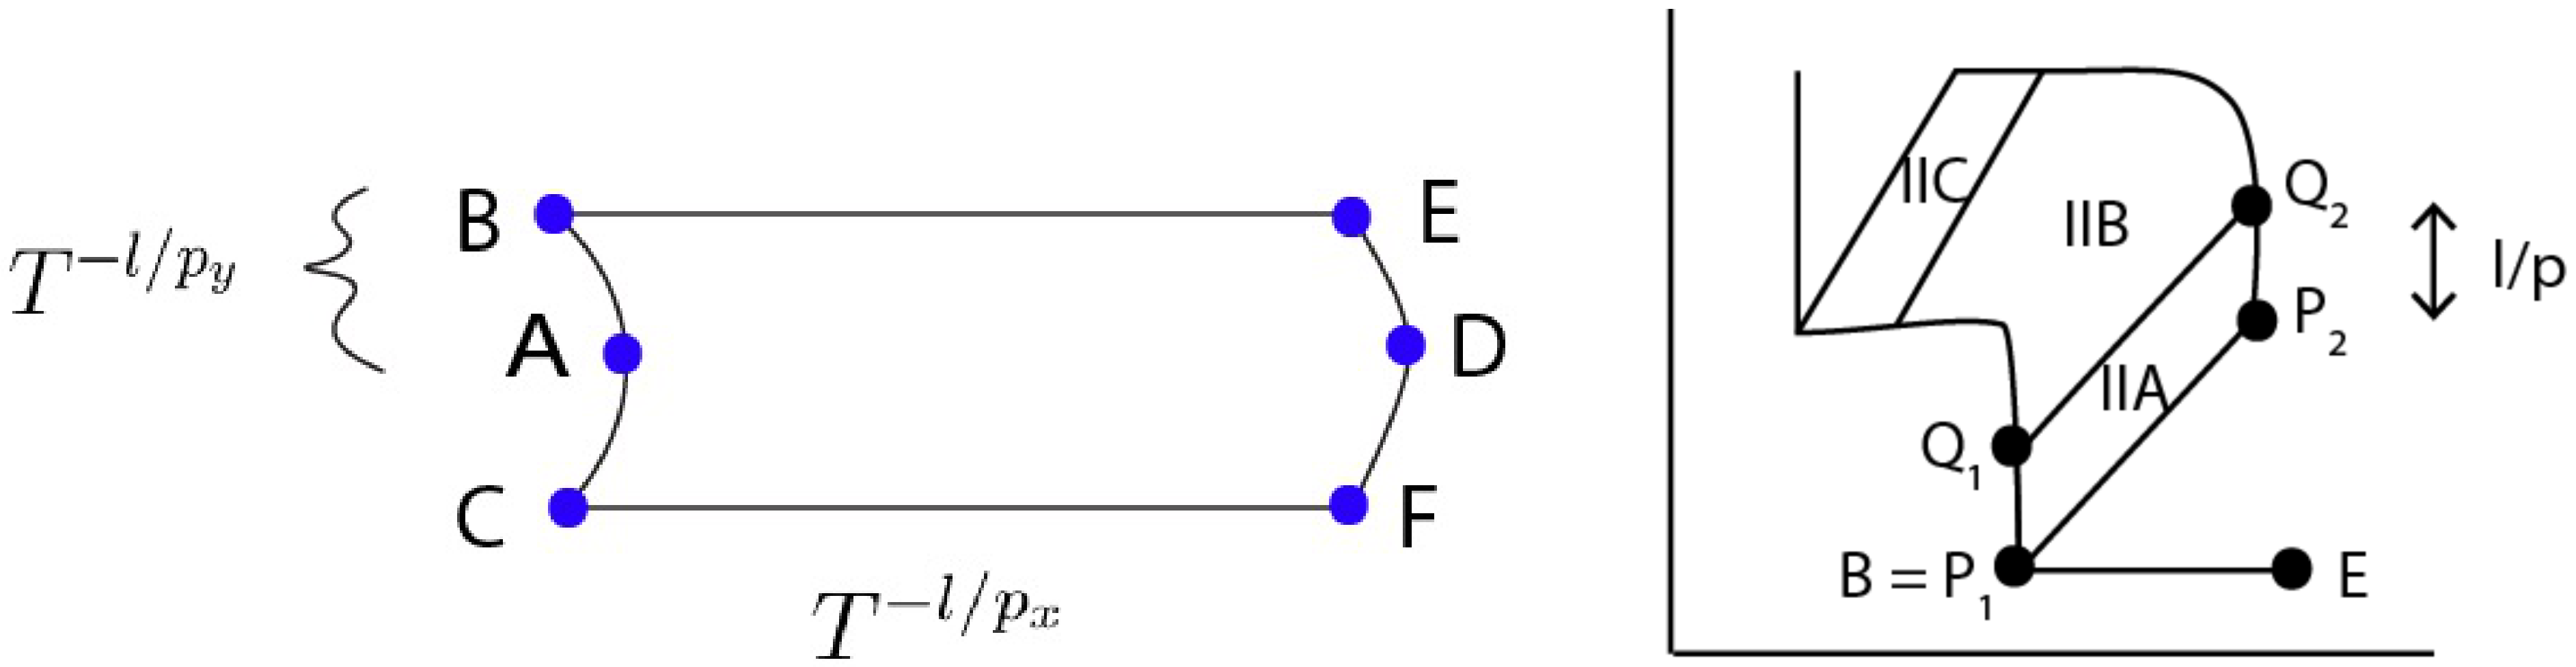
\includegraphics[width=0.95\textwidth]{figures/fig_1_9.png}
  \caption{左、右两图分别是区域 I 与区域 II 的放大。（原书 p.37）}
  \label{fig:1-9}
\end{figure}

\noindent\textbf{区域 I}
\begin{itemize}[leftmargin=2.2em,itemsep=0.25em]
\item $A(r_x,r_y,r_z)=(T^{l/4},T^{3l/8},T^{3l/8})$。
\item $B(r_x,r_y,r_z)\approx(T^{l/4},T^{3l/8-l/p},T^{3l/8+l/p})$。
\item $C(r_x,r_y,r_z)\approx(T^{l/4},T^{3l/8+l/p},T^{3l/8-l/p})$。
\item $D(r_x,r_y,r_z)=(T^{l/4-l/p},T^{3l/8+l/2p},T^{3l/8+l/2p})$。
此处 $r_x$ 已增大，而 $r_y=r_z$ 保持不变。
\item $E(r_x,r_y,r_z)\approx(T^{l/4-l/p},T^{3l/8-l/p},T^{3l/8+2l/p})$。
\item $F(r_x,r_y,r_z)\approx(T^{l/4-l/p},T^{3l/8+2l/p},T^{3l/8-l/p})$。
\end{itemize}

划分区域 II 的曲线为：沿径向向外的直线 $\theta_{II}$ 为常数，
沿角向曲线 $d_{IIA}$ 或 $d_{IIB}$ 为常数。
注意此处 $d_{IIA}$ 为常数近似于 $r_x$ 为常数。

\noindent\textbf{区域 II}
\begin{itemize}[leftmargin=2.2em,itemsep=0.25em]
\item $P_1=B\approx(T^{l/4},T^{3l/8-l/p},T^{3l/8+l/p})$。
\item $P_2\approx(T^{l/4-l/p},T^{3l/8-2l/p},T^{3l/8+3l/p})$。
\end{itemize}
这是因为从 $P_1$ 到 $P_2$ 的窄条上 $\theta_{II}=\log_T r_y-\log_T r_x$ 为常数；
而 $P_2$ 由沿 $d_I\approx(Tr_x)^2$ 常数的方向把 $E$ 上移得到，
故 $r_x(P_2)\approx T^{l/4-l/p}$。于是 $\theta_{II}$ 为常数给出
\begin{align*}
\theta_{II}(P_1)&\approx3l/8-l/p-l/4=l/8-l/p\\
&=\theta_{II}(P_2)\approx\log_T r_y-(l/4-l/p)\\
\Longrightarrow\ \log_T r_y&\approx3l/8-2l/p.
\end{align*}

% ===== 原书 p.38 =====
\begin{itemize}[leftmargin=2.2em,itemsep=0.25em]
\item $Q_1\approx(T^{l/4},T^{3l/8-2l/p},T^{3l/8+2l/p})$。
从 $P_1$ 沿 $d_{IIA}$ 常数到 $Q_1$，$r_y$ 乘以 $T^{-l/p}$，而 $r_x$ 近似不变。
\item $Q_2\approx(T^{l/4-l/p},T^{3l/8-3l/p},T^{3l/8+4l/p})$。
从 $Q_1$ 到 $Q_2$，$\theta_{II}$ 为常数；在 $Q_1$ 处
$\theta_{II}(Q_1)\approx3l/8-2l/p-l/4=l/8-2l/p$。
从 $P_2$ 到 $Q_2$，$r_x$ 近似不变，故 $Q_2$ 处 $\log_T r_x$ 近似为 $l/4-l/p$，于是
\[
\log_T r_y\approx(l/8-2l/p)+(l/4-l/p)=3l/8-3l/p.
\]
\end{itemize}
$r_z$ 坐标由 $r_xr_yr_z=T^l$ 确定。

现在终于得到关于 $p$ 的条件。我们希望区域 IIA 中处处 $r_x\gg r_y$，
使 $d_{IIA}$ 的等值线大致如所画，且 $d_{IIA}$ 的近似成立。
看 $Q_1$，这意味着 $T^{l/4}\gg T^{3l/8-2l/p}$；$Q_2$ 给出同样的限制。
故需 $1/8-2/p>0$，即 $p>16$。例如取 $p=17$。

其余区域由对称性定义。

\transnote{$p$ 的作用是把区域 IIA 的坐标细化到可分辨的程度；条件 $p>16$ 来自 $r_x\gg r_y$ 的要求，即比较 $Q_1$ 处的 $T^{l/4}$ 与 $T^{3l/8-2l/p}$。取 $p=17$ 只是方便的选取，不影响几何。}

\subsection{辛形式的定义}

现在定义 $H=\Sigma_2$ 情形下的辛形式。

\begin{figure}[htbp]
  \centering
  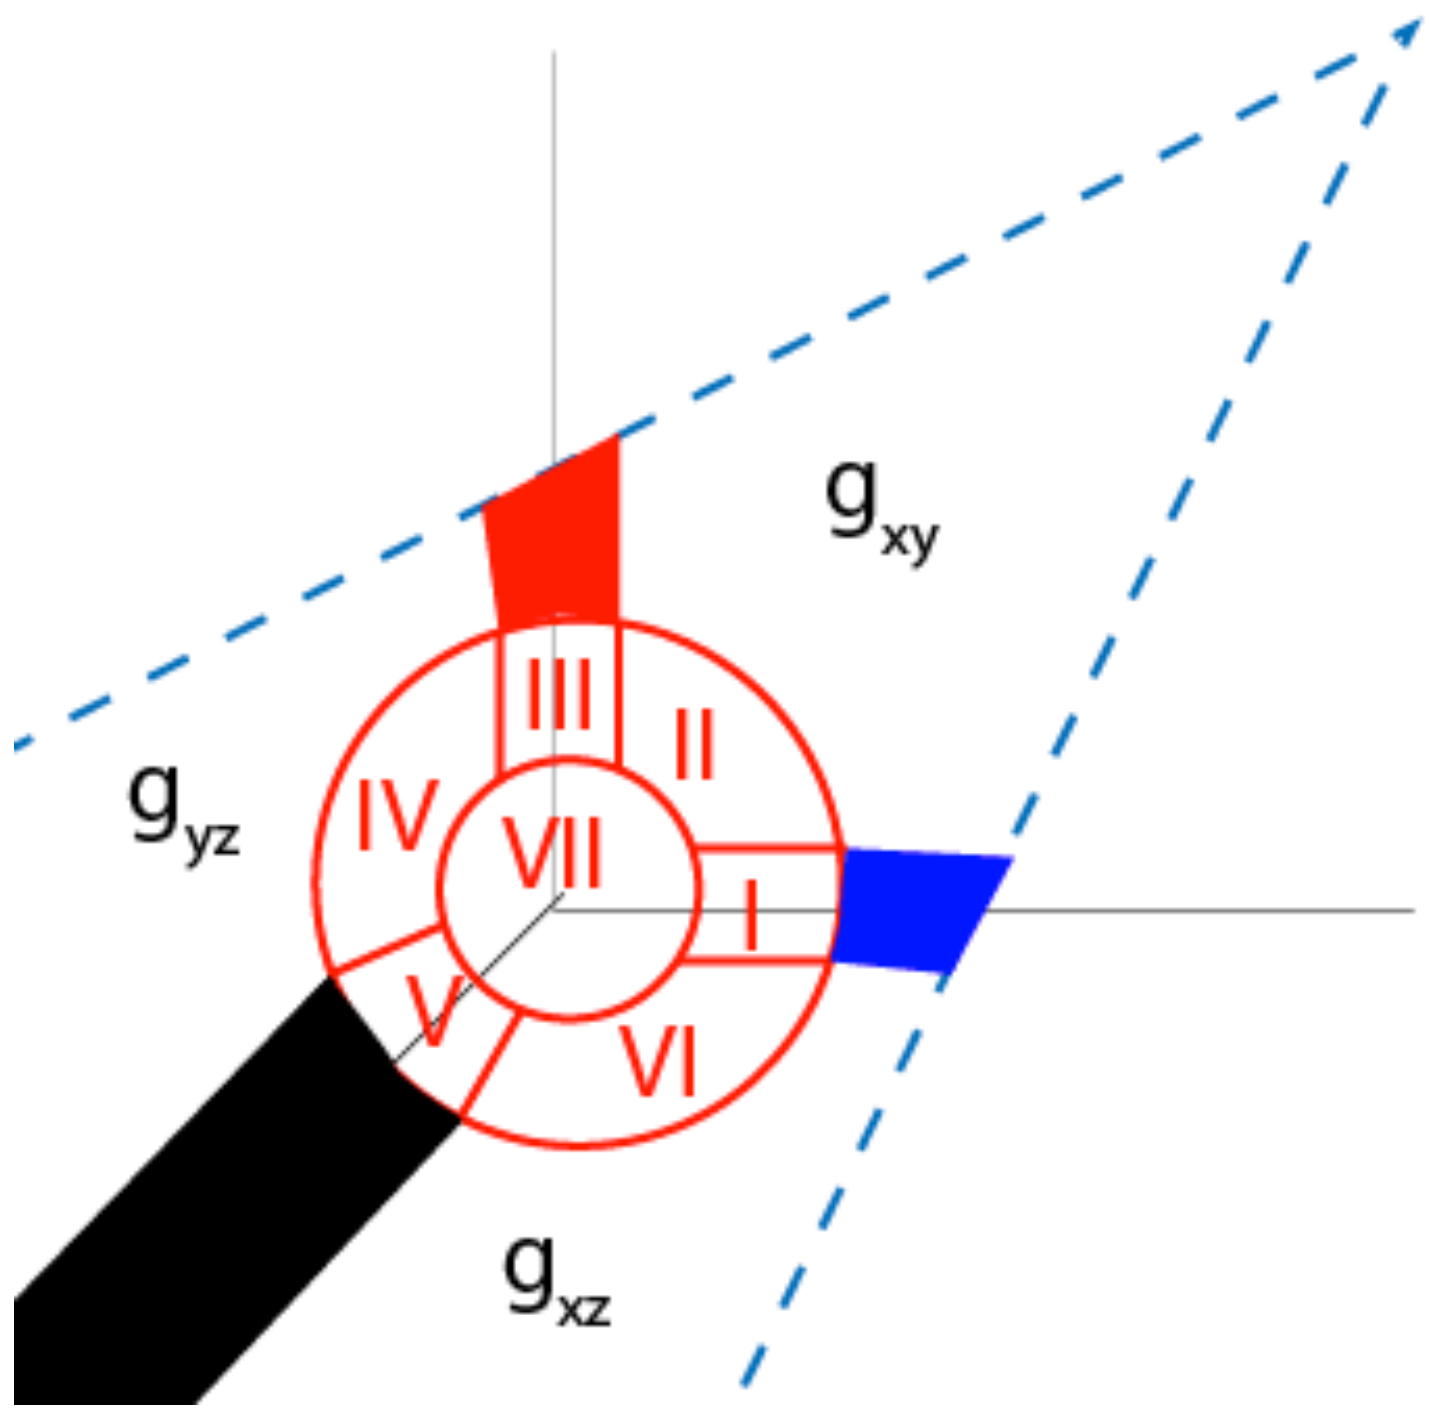
\includegraphics[width=0.38\textwidth]{figures/fig_1_10.png}
  \caption{在三个势之间插值：$F=\alpha_1g_{xy}+\alpha_2g_{xz}+(1-\alpha_1-\alpha_2)g_{yz}$，
  $0\le\alpha_1,\alpha_2\le1$。区域 VII 是 $\alpha_1=\alpha_2=1/3$ 之处；
  由对数近似，$F=\frac13(g_{xy}+g_{xz}+g_{yz})\approx\frac23((Tr_x)^2+(Tr_y)^2+(Tr_z)^2)$。
  （原书 p.38）}
  \label{fig:1-10}
\end{figure}

% ===== 原书 p.39 =====
\begin{definition}[辛形式的定义]\label{def:symplectic-form}
置 $\omega=\frac{i}{2\pi}F$，其中 $F$ 局部地由式~\eqref{eq:1-18} 的坐标定义如下：
\begin{equation}\label{eq:1-21}
\begin{gathered}
g_{yz}=\log(1+|Ty|^2)(1+|Tz|^2)(1+|T^2yz|^2),\\
g_{xz}=\log(1+|Tx|^2)(1+|Tz|^2)(1+|T^2xz|^2),\\
g_{xy}=\log(1+|Tx|^2)(1+|Ty|^2)(1+|T^2xy|^2).
\end{gathered}
\end{equation}
引入新的鼓包函数 $\alpha_3,\dots,\alpha_6$ 如下：
\[
\frac23\le\alpha_3(d_I)=\alpha_1+\alpha_2\le1,\qquad
-\frac12\le\alpha_4(\theta_I)\le\frac12,\qquad
0\le\alpha_5(d_I)\le1,\qquad
0\le\alpha_6(\theta_{II})\le1,
\]
\[
\alpha_4(\theta_I)\cdot\alpha_5(d_I)=\frac12(\alpha_1-\alpha_2).
\]
这些鼓包函数光滑、作为指定变量的函数递增，
且在定义域两端附近取所给界值的常数。
我们还要求 $\alpha_4$ 是奇函数。
关于这些鼓包函数性质的解释，见下小节「定义的动机」。
现在定义如下；注意 $g_{xz}-g_{yz}=\phi_x-\phi_y$，且 $(x,y,z)$ 的轮换同理：
\begin{equation}\label{eq:1-22}
\begin{gathered}
\text{图 1.10 中的区域 } g_{\bullet}\text{：分别对应 }F=g_{xy},\ F=g_{yz},\ F=g_{xz}\\
\text{区域 I：}\quad F=g_{yz}+\alpha_3(d_I)d_I+\alpha_4(\theta_I)\alpha_5(d_I)\theta_I\\
\text{区域 IIA：}\quad F=g_{yz}-\alpha_6(\theta_{II})\phi_y+\alpha_3(d_{IIA})d_{IIA}\\
+\frac12\alpha_5(d_{IIA})\bigl(\phi_y-\phi_z-\alpha_6(\theta_{II})\phi_y\bigr)\\
\text{区域 IIB：}\quad F=(g_{yz}-\phi_y)+\alpha_3(d_{IIB})d_{IIB}-\frac12\alpha_5(d_{IIB})\phi_z\\
\text{区域 IIC：}\quad F=g_{xz}-\alpha_6(-\theta_{II})\phi_x+\alpha_3(d_{IIC})d_{IIC}\\
+\frac12\alpha_5(d_{IIC})\bigl(\phi_x-\phi_z-\alpha_6(-\theta_{II})\phi_x\bigr)\\
\text{区域 I 到区域 IIA：}\quad F=g_{yz}+\alpha_3(d_I)\cdot d_I+\frac12\alpha_5(d_I)\cdot\theta_I\\
=g_{yz}+\alpha_3(d_{IIA})d_{IIA}+\frac12\alpha_5(d_{IIA})\cdot\theta_I\\
\text{区域 VII：}\quad F=\frac13(g_{xy}+g_{xz}+g_{yz})
\end{gathered}
\end{equation}

这些公式在边界处互相匹配，因此可以用 $(x,y,z)$ 的置换，
把区域 III–VI 像 I、II 那样由对称性定义。
例如可以验证：区域 IIA 的公式在 $\alpha_3=\frac23$、$\alpha_5=0$ 时与区域 VII 的公式一致；
在 $\alpha_6=0$、$\alpha_4=\frac12$ 时与区域 I 的一致；
在 $\alpha_6=1$ 时与区域 IIB 的一致；在 $\alpha_3=\alpha_5=1$ 时与 $g_{xy}$ 一致。
其余区域的计算类似。
\end{definition}

沿坐标轴（即染成红、蓝、黑色的区域），
我们用与区域 I、III、V 相同的公式、取 $\alpha_3\equiv1$，在相应的 $g_{\bullet}$ 之间插值。
例如沿 $r_x$ 轴（蓝色区域），公式为
$F=\frac12(g_{xy}+g_{xz})+\alpha_4(\theta_I)(g_{xy}-g_{xz})$；其余边类似。

\transnote{$\alpha_4\cdot\alpha_5=\frac12(\alpha_1-\alpha_2)$ 把两个鼓包函数捆绑在一起：$\alpha_5$ 控制径向支撑，$\alpha_4$ 控制角向变化。边界匹配正是靠这一乘积条件与 $\alpha_4$ 的奇性。}

% ===== 原书 p.40 =====
由于凯勒势是局部定义的，且在 $(\xi_1,\xi_2)$ 坐标中原点邻域内关于 $(x,y,z)$ 对称，
我们可以要求凯勒形式在先前所述 $\Z/6$-作用与 $\Gamma_B$-作用下都不变，从而处处定义它。
这一相容性条件在下面的断言~\ref{clm:descends} 中验证。

辛形式的定义到此完成。

\medskip\noindent\textbf{定义的动机}\par

我们可以重新整理 $F$ 的初始表达式中依赖于 $\alpha_1,\alpha_2$ 的项，
以说明 $\alpha_3$ 与 $\alpha_4\cdot\alpha_5$ 的定义，以及各区域中 $d$ 与 $\theta$ 的定义。
$\alpha_6$ 的选取与区域 II 中的变量，是为了在两侧（即区域 I 与 III）$F$ 的定义之间插值。
\begin{align*}
F&=\alpha_1g_{xy}+\alpha_2g_{xz}+(1-\alpha_1-\alpha_2)g_{yz}\\
&=\alpha_1\log(1+|Tx|^2)(1+|Ty|^2)(1+|T^2xy|^2)
+\alpha_2\log(1+|Tz|^2)(1+|Tx|^2)(1+|T^2xz|^2)\\
&\quad+(1-\alpha_1-\alpha_2)\log(1+|Tz|^2)(1+|Ty|^2)(1+|T^2yz|^2)\\
&=g_{yz}+(\alpha_1+\alpha_2)\phi_x
-\Bigl(\frac{\alpha_1+\alpha_2}{2}-\frac{\alpha_1-\alpha_2}{2}\Bigr)\cdot\phi_y
-\Bigl(\frac{\alpha_1+\alpha_2}{2}+\frac{\alpha_1-\alpha_2}{2}\Bigr)\cdot\phi_z\\
&=g_{yz}+(\alpha_1+\alpha_2)\bigl(\phi_x-\tfrac12(\phi_y+\phi_z)\bigr)
+\tfrac12(\alpha_1-\alpha_2)(\phi_y-\phi_z).
\end{align*}

注意 $\alpha_1,\alpha_2,1-\alpha_1-\alpha_2$ 并不对称，但三者应被对称地对待，
故如上合并。换言之，把 $(\alpha_1,\alpha_2)$ 看作向量并旋转 $\pi/4$，得到与
\[
\begin{pmatrix}1&-1\\1&1\end{pmatrix}
\begin{pmatrix}\alpha_1\\\alpha_2\end{pmatrix}
=\begin{pmatrix}\alpha_1-\alpha_2\\\alpha_1+\alpha_2\end{pmatrix}
\]
成比例的向量。

\transnote{把 $\alpha_1g_{xy}+\alpha_2g_{xz}+(1-\alpha_1-\alpha_2)g_{yz}$ 按三个 $\log$ 因子重新分组；$g_{yz}$ 之外的项恰好组合成 $\phi_x-\frac12(\phi_y+\phi_z)$ 与 $\phi_y-\phi_z$，这就是 $d_I$ 与 $\theta_I$ 的来源。}

定义 $\alpha_3=\alpha_1+\alpha_2$。为得到其界，我们考虑几何以及 $\alpha_1,\alpha_2$ 的变化。
在中心区域 VII 中 $\alpha_1=\alpha_2=1/3$。
沿 $r_x$ 方向穿过区域 I 到达尽头时，不应有 $g_{yz}$ 贡献，
即那里 $\alpha_3=\alpha_1+\alpha_2=1$。于是区域 I 中 $\alpha_3$ 从 $2/3$ 变到 $1$。

我们用 $\alpha_1-\alpha_2$ 定义角向变化的鼓包函数 $\alpha_4$，
其角向变量记作 $\theta_I$，定义见下文。这里有一处需要注意。
在区域 I 起点 $\alpha_1=\alpha_2=1/3$，故沿角 $\theta_I$ 走时 $\alpha_1-\alpha_2$ 始终为 $0$；
但在区域 I 末端，从底部的 $(\alpha_1,\alpha_2)=(0,1)$ 走到顶部的 $(1,0)$，
于是 $\alpha_1-\alpha_2$ 在 $-1$ 与 $1$ 之间变化。
因此需把 $\alpha_4(\theta_I)$ 乘以另一个鼓包函数 $\alpha_5(d_I)$；
后者从 $0$ 变到 $1$，依赖于随 $r_x$ 增大而增大的变量 $d_I$，下文将定义。
于是我们缩放了 $\alpha_4$ 的变化区间。出于对称性，要求 $\alpha_4$ 是奇函数。
% ===== 原书 p.41 =====
令 $\alpha_4\cdot\alpha_5=\frac12(\alpha_1-\alpha_2)$，于是
\[
F=g_{yz}+\alpha_3\bigl(\phi_x-\tfrac12(\phi_y+\phi_z)\bigr)+\alpha_4\cdot\alpha_5(\phi_y-\phi_z).
\]

后续计算的关键在于：鼓包函数会乘以它所依赖的变量。
$\alpha_i$ 依据「绕圆走了多远」（角向）与「离中心多远」（径向）变化。
于是我们引入一组坐标 $d$ 与 $\theta$，它们可从上面 $F$ 的表达式读出：
$d_I=\phi_x-\frac12(\phi_y+\phi_z)$，$\theta_I=\phi_y-\phi_z$。
下面从几何上说明它们为何合理。

我们想构造一个辛形式，使其矩多面体由 Delzant 定理与环簇多面体相同。
从图中能读出的是 $r_x,r_y,r_z$ 彼此如何比较；
即使无法确定其值，也可观察它们的相对大小。
特别地，在图~\ref{fig:1-11} 中可见：$T^2(r_y^2-r_z^2)$ 沿向上的竖直方向增大，
$(Tr_x)^2$ 沿向右的水平方向增大。
这启发了我们对角向与径向变量的选取；这些变量可用首阶项近似。

\begin{figure}[htbp]
  \centering
  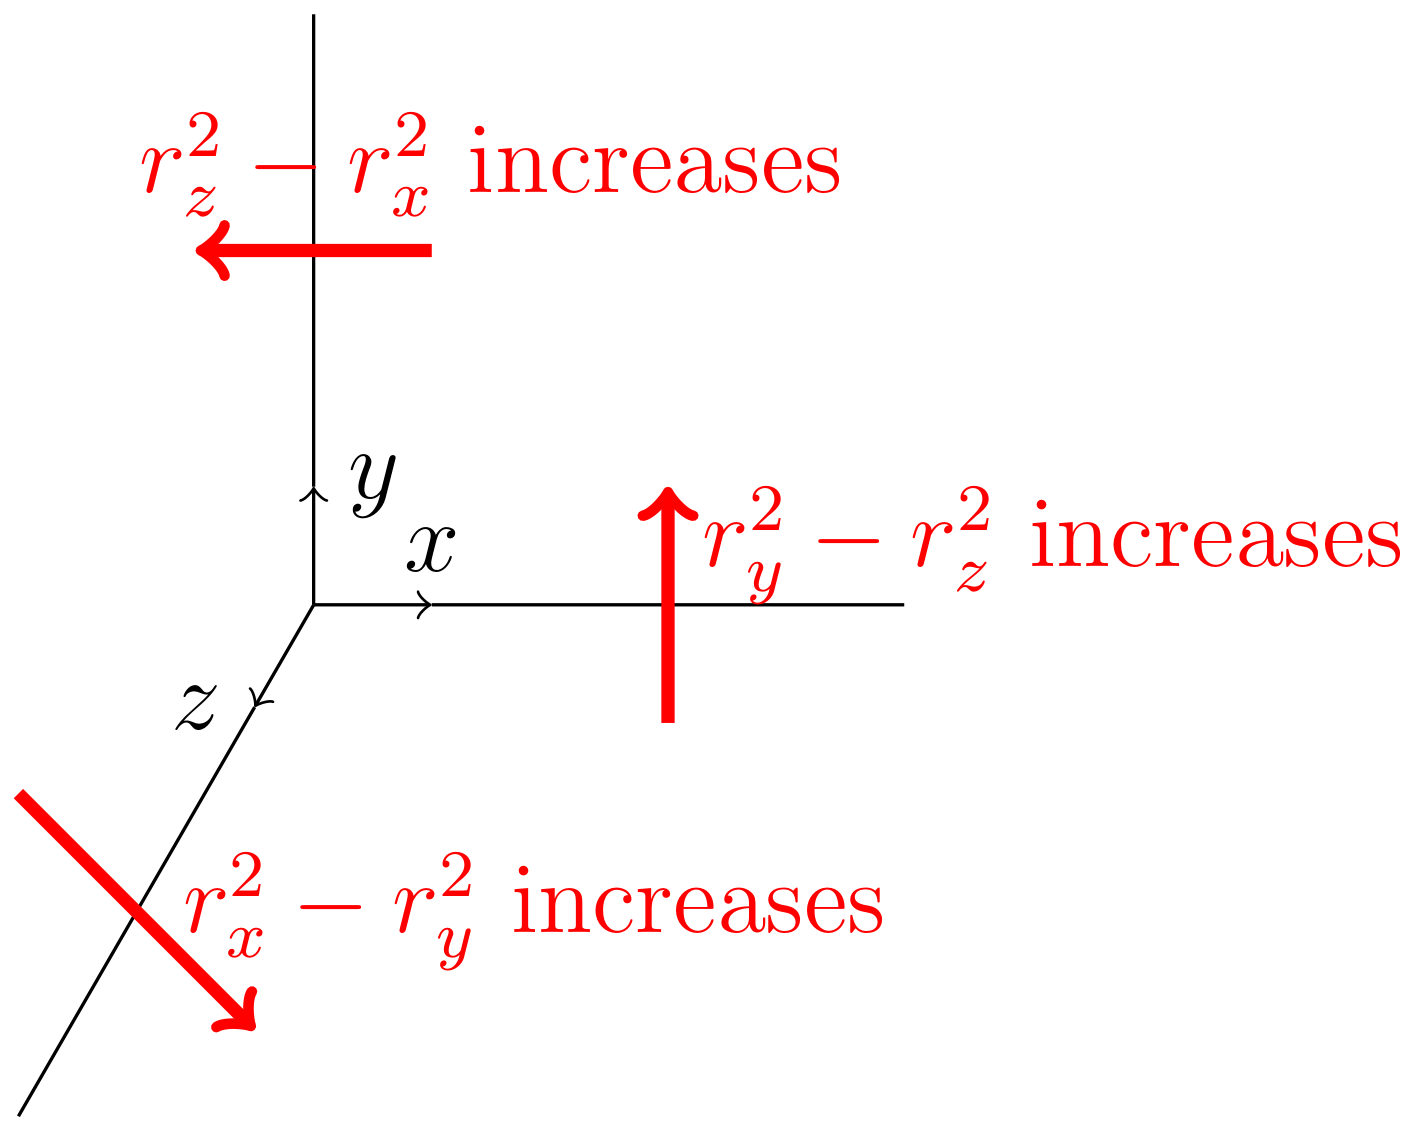
\includegraphics[width=0.4\textwidth]{figures/fig_1_11.png}
  \caption{三条角向如何变化。（原书 p.41）}
  \label{fig:1-11}
\end{figure}

在区域 I 中，$d$ 应随 $x$ 增大。
具体地，$d_I:=\phi_x-\frac12(\phi_y+\phi_z)$ 仍随 $x$ 增大，
因为区域 I 开始时 $r_x\gg r_y,r_z$。
（由于 $v_0=xyz$，固定纤维时 $|x|$ 增大意味着 $|yz|$ 相应减小。）

对角度方向，注意在表达式 $\phi_x:=\log(1+|Tx|^2)/(1+|T^2yz|^2)$ 中，
首阶项是 $|Tx|^2$。于是如上所述，$\theta_I=\phi_y-\phi_z$ 应是角向坐标，从而得到
\[
F=g_{yz}+\alpha_3(d_I)\cdot d_I+\alpha_4(\theta_I)\cdot\alpha_5(d_I)\cdot\theta_I.
\]
至此定义了区域 I 中的凯勒势。由 $(x,y,z)$ 的对称性，它也定义了区域 III 与 V 中对应的势。
随后区域 II 在这些势之间插值。

% ===== 原书 p.42 =====
\medskip\noindent\textbf{$\omega$ 延拓过中心纤维并下降到 $Y$}\par

由于 $\omega$ 的构造，该形式延拓为全空间上的形式，包含零纤维。
若在顶点周围画一个圆盘并考虑其上所有 $|v_0|$ 值，
就得到 $\C^3$ 中的一块，其凯勒形式在 $r_x,r_y,r_z$ 小时近似标准辛形式；
也就是说，我们移植了 $(\C^3,xyz)$ 模型纤维丛的一部分，
而它是光滑流形、有良定义的辛形式。
若在六边形中心取一个圆盘形区域，那里只有一个凯勒势起作用，
再考虑其上所有 $|v_0|$，就得到纤维中的模型环簇凯勒形式；
再加上来自纤维丛 $v_0$ 底空间的一项，便得到乘积辛形式。

在这两者之间插值的区域中，得到两个正定凯勒势的凸线性组合。
特别地，可取 $\epsilon$ 充分小，使给这两个度量之一加上 $\epsilon$ 不影响正定性。
然后固定 $l$ 的取值，使某些 $|v_0|=T^l$ 时下文所述所有鼓包函数导数都小于 $\epsilon$。
之后可令 $|v_0|=T^{l'}$ 趋于零，而界仍然成立：若对 $l$ 成立，则 $l'\to\infty$ 时只会更小。
换言之，一旦为鼓包函数导数留出足够空间，
就可以定义它们在所有 $v_0\to0$ 的纤维上有相同的支集，并在其余部分为常数。

此外，$\omega$ 以 $\Gamma_B$-不变（也以 $\Z/6$-不变）的方式延拓到整个 $\tilde Y$：
用群作用在定义~\ref{def:Y} 引入的其他坐标卡 $U_{n,g^k}$ 中定义它。
于是这些公式在卡的重叠处相符，给出 $\tilde Y$ 上良定义的 2-形式。
进一步，它如下下降到商 $Y$ 上良定义的 2-形式。

\begin{claim}\label{clm:descends}
形式 $\omega$ 下降到商 $Y=\tilde Y/\Gamma_B$ 上良定义的 2-形式。
\end{claim}

\begin{proof}
上面已见 $\omega$ 的局部模型良定义，因为所有局部定义在边界处一致；
这一点在定义~\ref{def:symplectic-form} 末尾已指出。
此外，在 $\Delta_{\tilde Y}$ 的每个顶点与六边形瓦片中心粘合坐标卡 $U_{n,g^k}$
（见定义~\ref{def:Y}）时，公式一致。
例如引理~\ref{lem:interpolation} 证明 $g_{xy}$ 在 $\Z/6$-作用下对称。
最后，沿边的定义必须相容。换言之，取 $\alpha_3=\alpha_5=1$，
从区域 I、III、V 延拓到图 ?? 中染成黑、红、蓝的阴影区域时，变换是相容的。
% [Tutor Note: 原文作「of Figure ??」，是坏引用；按上下文应为图 1.10。保留原样，登记为疑点。]
由对称性，只需沿 $r_z$ 轴检验。
按定义~\ref{def:Y} 的记号，这是主卡 $U_{0,g^0}$（坐标 $(x,y,z)$）
与坐标卡 $U_{(-1,0),g^{-1}}$（坐标 $(x''',y''',z''')=(Tyz,Txz,T^{-2}z^{-1})$）之间的变换。

设 $F$ 为未加撇坐标中辛形式的凯勒势，$F'''$ 为三撇坐标中的凯勒势。
在我们考虑的区域，$F$ 由区域 V 的公式在 $\alpha_3=\alpha_5=1$ 时给出。

% ===== 原书 p.43 =====
\begin{align*}
F_V&=g_{xy}+d_V+\alpha_4(\theta_V)\cdot\theta_V\\
g_{xy}+d_V&=\log_T(1+|Tx|^2)(1+|Ty|^2)(1+|T^2xy|^2)\cdot\\
&\quad\Biggl(\frac{1+|Tz|^2}{1+|T^2xy|^2}\Bigg/
\sqrt{\frac{1+|T^2xz|^2}{1+|Ty|^2}\cdot\frac{1+|T^2yz|^2}{1+|Tx|^2}}\Biggr)\\
&=\frac12\log_T(1+|Tx|^2)(1+|Ty|^2)(1+|T^2xz|^2)(1+|T^2yz|^2)
+\log_T(1+|Tz|^2)\\
\theta_V&=\phi_x-\phi_y\\
\therefore\ g'''_{xy}&=\Bigl(\frac12\log_T(1+|T^2yz|^2)(1+|T^2xz|^2)(1+|Ty|^2)(1+|Tx|^2)
+\log_T(1+|T^{-1}z^{-1}|^2)\Bigr)\\
&\quad+\alpha_4(-\theta_V)\cdot(-\theta_V)\\
&=g_{xy}-\log_T(|Tz|^2).
\end{align*}
最后等号成立：第一项中，用 $(x,y,z)$ 与 $(x''',y''',z''')$ 之间的坐标变换作拉回，
只是置换因子；第二项用 $\alpha_4(-\theta)=-\alpha_4(\theta)$。
又注意在该坐标卡下 $\theta_V'''$ 对应 $-\theta_V$。
于是从一个卡到另一个卡需加 $\log_T(|Tz|^2)$；
它是调和函数，因为 $\log(Tz)$ 全纯而其共轭反全纯。
\end{proof}

\transnote{「延拓过中心纤维」与「下降到商」是两件不同的事：前者用 $(\C^3,xyz)$ 局部模型补上零纤维处的定义，后者验证 $\Gamma_B$-不变性。至于 $\omega$ 闭且非退化、以及正定性，引理~\ref{lem:symplectic-on-Y} 把它们留到第 2 章。}

\begin{lemma}\label{lem:symplectic-on-Y}
$\omega$ 的定义给出 $Y$ 上良定义的辛形式。
\end{lemma}

其完整证明在下一章，将证明正定性。

% EN48 c04 | 原书 原书 p.44–69（PDF 53–78） | 第 2 章 §2.1–2.4
% 骨架文件：标题行已设定，正文由译者填写。每页起首用 % ===== 原书 p.N ===== 注释标记。
\section{辛形式 $\omega$ 的非退化性}

% ===== 原书 p.44 =====
本章的目标是证明：

\begin{lemma}\label{lem:omega-fiber}
第 1.5 节定义的 $\omega$，在由 $v_0\colon Y\to\C$ 给出的 Landau–Ginzburg 模型的纤维上非退化。
\end{lemma}

\begin{corollary}\label{cor:omega-y}
在底空间上添加一项，由此得到 $Y$ 上的非退化形式 $\omega$。
\end{corollary}

\transnote{本章只论证 $\omega$ 的非退化，不直接论证正定性：正定性要靠再往凯勒势里加底空间的一项 $|xyz|^2$ 来补（见原书 p.50 与 p.56 的两处说明）。读后面的长计算时，凡是出现「某一项趋于零」的段落，都要记住补这一项之后才得到度量的正定。}

\subsection{对鼓包函数导数给出界}

\begin{claim}[对数导数便于作出估计]\label{claim:log-bounds}
设 $\alpha$ 取 $\alpha_3,\dots,\alpha_5$ 中的任一个，$\mu$ 为相应的 $d$ 或 $\theta$ 变量。那么可以保证：对数导数（logarithmic derivative）${\alpha'}^{\log}=\mu\alpha'(\mu)$ 在 $\log(T^l)$ 上被常数界住；二阶导数同理。$\alpha_6$ 的论证不同：它的自变量已经是复坐标范数的对数函数，因此通常的导数可以控制。
\end{claim}

特别地，$\log_T$ 导数可以取得很小。把凯勒势写成 $\alpha(\mu)\cdot\mu$ 的形式（$\alpha$、$\mu$ 取得合适），威力正在于此。本节考察鼓包函数的导数。一阶导数会拾取如下形式的项：
\[
\alpha'(\mu)\cdot\mu_*\cdot\mu=\mu_*\frac{d\alpha}{d(\log_T\mu)}
\approx(\text{small})\cdot\frac{\Delta\alpha}{\Delta\log_T\mu},
\]
其中 $\mu_*$ 是 $\mu$ 对某个坐标的某个导数。回忆 $\mu$ 将用 $T$ 乘范数的平方和来近似。这些范数非常小，量级为 $T^l$。然而 $\log_TT^l=l$，所以分子与分母都只变 $O(1)$ 项，再乘上一个可以取得很小的因子。特别是，我们除以 $l$，而 $l$ 想取多大就取多大。

% ===== 原书 p.45 =====
\begin{remark}[检验导数变小的空间是否足够，参看图 1.9]\label{rem:enough-space}
在区域 I 中 $d\approx T^2[r_x^2-\frac12(r_y^2+r_z^2)]>0$，因为进入该区域时 $r_x$ 比 $r_y$、$r_z$ 大许多个数量级。不过在 $\alpha_4$ 的计算里，最后要除以 $\theta$。所以 $\alpha_4$ 需要在中间一小段上保持常数，以免除以零。下文会详细交代。
\end{remark}

另外，$\theta_{II}$ 与 $\log d_{IIA}$ 中分别有足够的空间留给 $\alpha_6$ 与 $\alpha_3,\alpha_5$。回忆
\[
d_{IIA}\approx T^2\Big[r_x^2-\frac12(r_y^2+r_z^2)+\frac32\alpha_6\cdot r_y^2\Big].
\]
区域 IIA 内处处有 $r_x\gg r_y$，所以 $d_{II}$ 的主项是 $(Tr_x)^2$。同理，$\theta_{II}$ 关于 $\log_Tr_y-\log_Tr_x$ 线性；要让它保持常数，$\log_Tr_y$ 与 $\log_Tr_x$ 沿等值线就得增加相同的量。在 $P_1$、$P_2$ 处 $\theta_{II}\approx T^{3l/8-2l/p}$，在 $Q_1$、$Q_2$ 处 $\theta_{II}\approx T^{l/8-2l/p}$。于是变化量为 $2l/8=l/4$，且 $\alpha_6'\approx\Delta\alpha_6/\Delta\theta_{II}\approx4/l$。这可以取得很小。

现在对 $\alpha_3$、$\alpha_5$ 检验 $d_{IIA}$。在较小的取值处，$P_1$ 上 $d_{IIA}\approx(Tr_x)^2$，指数为 $l/2$；在较大的取值处指数为 $l/2-2l/p$。所以变化量是 $2l/p$，$\alpha_3$、$\alpha_5$ 中的导数约为 $\frac{p}{2l}$ 乘以 $\alpha_i$ 的整个取值范围。这同样可以取得很小。

二阶导数也有足够的空间。鼓包函数 $\alpha_3,\dots,\alpha_6$ 中，求导所沿的变量有 $k\cdot l$（某个 $k>0$）的移动空间，而每个鼓包函数只走过 $1/3$ 或 $1$ 的量。让 $l$ 足够大，就能保证这一过程中二阶导数不会太大。鼓包函数的图像不会是直的，因为它们必须在支撑集的端点处变平。但只要空间足够，就能保证它们从水平转向线性的过程不至于太急。

区域 IIC 中空间足够的论证，由 IIA 交换 $r_x$ 与 $r_y$ 得到。区域 IIB 中唯一的变量是 $d_{IIB}$；我们取两条径向曲线为 $d_{IIB}$ 的等值线，变量的变化量与 $d_{IIA}$ 中相同。注意当 $r_x\gg r_y$ 时
\[
d_{IIB}\approx T^2\Big[r_x^2+r_y^2-\frac12r_z^2\Big]\approx(Tr_x)^2.
\]
所以起初「$d_{IIB}$ 为常数」与「$r_x$ 为常数」近似是一回事。到某一步我们把 $r_y$ 增大到与 $r_x$ 相等。同理，从区域 IIC 过来时，「$d_{IIB}$ 为常数」起初近似等于「$r_y$ 为常数」。于是在中段，曲线从竖直（$r_x$ 为常数）插值到水平（$r_y$ 为常数）。$d_{IIB}$ 的函数有足够空间，因为 $d_{IIB}$ 走过的量与 $d_{IIA}$、$d_{IIC}$ 相同。

\medskip
\noindent\textbf{检验 ${\alpha_3'}^{\log}$ 与 ${\alpha_5'}^{\log}$ 足够小。} 区域 I 中 $\alpha_3$ 是
\[
T^2\Big[d_I\approx r_x^2-\frac12(r_y^2+r_z^2)\Big]\approx(Tr_x)^2
\]
的函数，所以要看 $\log_T(Tr_x)^2$ 如何变化。回忆 $r_x$ 变了 $l/p_x$ 个数量级，于是 $\log_T(Tr_x)^2$ 约变 $2l/p_x$。

% ===== 原书 p.46 =====
于是如上所述，对数导数可以取得任意小。

对 ${\alpha_3''}^{\log}$，我们要知道斜率在 $\log d$ 时间内的变化。导数在约 $l$ 的 $\log$ 时间内从 $0$ 变到 $\frac{1}{3l}$。想一个从 $2/3$ 到 $1$ 的鼓包函数。于是所有含 $\alpha_3$ 导数的项都被常数乘 $T^2/l$ 界住。

\medskip
\noindent\textbf{检验跨坐标轴的对数导数有足够空间。} 回忆图 1.9：从 $A$ 到 $B$，$r_y$ 走过 $l/p$ 个 $T$ 的量级；从 $D$ 到 $E$ 则走过 $3l/2p$，对小的 $T$ 而言这大得多。

在上面的计算中，我们挖掉了一块区域 $T<(r_y/r_z)^2<T^{-1}$，其中 $\alpha_4\equiv0$。为此要保证 $r_y$ 与 $r_z$ 至少相差一个数量级。区域 I 里这没问题：在 $B$ 与 $C$ 处 $r_y$、$r_z$ 相差许多个数量级，向外走到 $E$、$F$ 差距更大。（不过区域 II 里的情形反过来。也就是说，向外走时 $r_z$ 变小，$r_x$ 与 $r_y$ 变大，而 $r_y^2-r_x^2$ 为常数意味着它们会越来越靠近。）

\medskip
\noindent\textbf{检验 ${\alpha_4'}^{\log}$，它是 $\theta_I$ 的函数。} 这个量是 $\theta_I\approx T^2[r_y^2-r_z^2]$ 或其负值的函数。此外要在轴附近挖掉一条窄带 $T<(r_y/r_z)^2<1/T$，所以要检查剩余空间够不够。在 $C$、$F$ 所在的底部，$\theta_I\approx-r_z^2$，量级为 $-T^2(3l/8-l/p_y)$，如前所见。随后我们在 $r_z/r_y=1/\sqrt{T}$ 处停下。此时 $r_z$ 与 $r_y$ 基本相等，因为它们只差约一个 $T$ 量级，而且都很小。在某个固定的 $d_I$ 处有 $r_x\approx T^{l/4-tl/p_x}$，其中 $t$ 固定为 $0$ 与 $1$ 之间的某个数。于是 $r_z=\sqrt{T}^{-1}r_y$，且
\[
r_xr_yr_z=T^l\quad\Longrightarrow\quad T^{l/4-tl/p_x}\cdot r_y\cdot\sqrt{T}^{-1}r_y=T^l
\quad\Longrightarrow\quad r_y^2=\sqrt{T}\cdot T^{3l/4+tl/p_x}.
\]
因此
\[
\begin{aligned}
\theta_I&\approx T^2[r_y^2-r_z^2]
=T^2r_y^2\left(1-\left(\frac{r_z}{r_y}\right)^2\right)\\
&\approx T^2\sqrt{T}\cdot T^{3l/4+tl/p_x}(1-T^{-1})
\approx -T^{3l/4+tl/p_x+3/2},\quad\because T\ll1.
\end{aligned}
\]

我们挖掉这条窄带，是为了检查 $\theta_I$ 的变化，以确认 $\alpha_4$ 在对数导数上有足够空间。结果 $\theta_I$ 从量级 $3l/4-2l/p_y$ 降到量级 $3l/4+tl/p_x+3/2$。于是净变化为
\[
(3l/4-2l/p_y)-(3l/4+tl/p_x+3/2)=-l\left(\frac{2}{p_y}+\frac{t}{p_x}\right)+3/2,
\]
其中含 $l$ 的倍数。所以 $\alpha_4$ 的对数导数仍然没问题：这个量是对数导数的分母，靠 $l$ 可以取得很大。注意我们只在区域 I 中关心 $\alpha_4$，因为离开该区域进入区域 II 时它已经恒等于 $1/2$。

\subsection{化为极坐标}

% ===== 原书 p.47 =====
为定义度量，我们换成极坐标，在那里更方便。局部地，辛形式是 $\frac{i}{2\pi}\partial\bar\partial F$，其中 $F$ 是 $|x|$ 与 $|y|$ 的函数。于是要用实变换 $(r_x,\theta_x)\leftrightarrow(x_1,x_2)$ 改写 $\partial\bar\partial$ 中的导数，其中 $x=x_1+ix_2=r_xe^{i\theta_x}$，$y$ 同理。回忆 $\partial_x=\frac12(\partial_{x_1}-i\partial_{x_2})$。由 $\partial_{x_i}=\partial_{x_i}(r_x)\partial_{r_x}+\partial_{x_i}(\theta_x)\partial_{\theta_x}$ 得
\[
\frac{\partial}{\partial x}
=\frac12\left(\frac{\partial}{\partial x_1}-i\frac{\partial}{\partial x_2}\right)
=\frac12\left(\left[\frac{\partial r_x}{\partial x_1}-i\frac{\partial r_x}{\partial x_2}\right]\frac{\partial}{\partial r_x}
+\left[\frac{\partial r_x}{\partial x_1}-i\frac{\partial r_x}{\partial x_2}\right]\frac{\partial}{\partial\theta_x}\right).
\]
% [Tutor Note: 原文第二个方括号内写作 ∂r_x/∂x_i，按上下文应为 ∂θ_x/∂x_i；照录不改。]
\transnote{上式右侧第二个方括号照录原文。按 $\partial_{x_i}=\partial_{x_i}(r_x)\partial_{r_x}+\partial_{x_i}(\theta_x)\partial_{\theta_x}$，这一处应为 $\partial\theta_x/\partial x_i$；若按字面代入，$x$ 方向的导数会对不上下一段的 $e^{-i\theta_x}$ 系数。}

接下来用极坐标 $r_x^2=x_1^2+x_2^2$ 与 $\theta_x=\tan^{-1}(x_2/x_1)$ 逐个改写实偏导数，$y$ 同理。回忆 $\arctan t$ 的导数是 $1/(1+t^2)$。
\[
\frac{\partial}{\partial x_1}=\frac{\partial r_x}{\partial x_1}\frac{\partial}{\partial r_x}+\frac{\partial\theta_x}{\partial x_1}\frac{\partial}{\partial\theta_x},
\qquad
r_x\frac{\partial r_x}{\partial x_i}=x_i\quad\Longrightarrow\quad\frac{\partial r_x}{\partial x_i}=\frac{x_i}{r_x},
\]
\[
\frac{\partial\theta_x}{\partial x_1}=-\frac{x_2}{r_x^2},\qquad
\frac{\partial\theta_x}{\partial x_2}=\frac{x_1}{r_x^2}.
\]
因此
\[
\frac{\partial}{\partial x}=\frac12\left[e^{-i\theta_x}\partial_{r_x}-ie^{-i\theta_x}/r_x\,\partial_{\theta_x}\right],
\qquad
\frac{\partial}{\partial\bar x}=\frac12\left[e^{i\theta_x}\partial_{r_x}+ie^{i\theta_x}/r_x\,\partial_{\theta_x}\right].
\]

$y$ 同理。还需要改写微分 $dx=dx_1+idx_2$ 与 $d\bar x$。用
\[
x_1=r_x\cos\theta_x,\qquad x_2=r_x\sin\theta_x,
\]
\[
\therefore\quad dx=e^{i\theta_x}dr_x+ir_xe^{i\theta_x}d\theta_x,\qquad
d\bar x=e^{-i\theta_x}dr_x-ir_xe^{-i\theta_x}d\theta_x.
\]

% ===== 原书 p.48 =====
现在把 $\partial\bar\partial F$ 化成极坐标。
\begin{align*}
i\partial\bar\partial F
&=\sum_{i,j=1}^{3}\frac{\partial^2F}{\partial z_i\partial\bar z_j}\,dz_i\wedge d\bar z_j\\
&=i\sum_{i,j}\Big(\tfrac12e^{-i\theta_{z_i}}\big[\partial_{r_{z_i}}-i/r_{z_i}\partial_{\theta_{z_i}}\big]\Big)
\Big(\tfrac12e^{i\theta_{z_j}}\big[\partial_{r_{z_j}}+i/r_{z_j}\partial_{\theta_{z_j}}\big]\Big)(F)\\
&\qquad\cdot\big(e^{i\theta_i}(dr_i+ir_i\,d\theta_i)\big)\wedge\big(e^{-i\theta_j}(dr_j-ir_j\,d\theta_j)\big)\\
&=i\tfrac14\sum_{i,j}e^{-i\theta_i}\Big[e^{i\theta_j}\partial^2_{r_ir_j}F
-\frac{i}{r_i}\partial_{r_j}F\,\delta_{ij}ie^{i\theta_j}\Big]
\big(e^{i\theta_i}(dr_i+ir_i\,d\theta_i)\big)\wedge\big(e^{-i\theta_j}(dr_j-ir_j\,d\theta_j)\big)\\
&=i\tfrac14\Big[\sum_i\Big(\partial^2_{r_i}F+\frac{1}{r_i}\partial_{r_i}F\Big)
(dr_i+ir_i\,d\theta_i)\wedge(dr_i-ir_i\,d\theta_i)\Big]\\
&\qquad+\tfrac14\Big[\sum_{i\ne j}\big(\partial^2_{r_ir_j}F\big)
(dr_i+ir_i\,d\theta_i)\wedge(dr_j-ir_j\,d\theta_j)\Big].
\end{align*}

为使上式来自一个度量，需要与 $J_0$ 相容，其中 $J_0$ 由环簇卡（toric chart）上复坐标 $(x,y,z)$ 乘以 $i$ 诱导。而 $\omega$ 与 $J$ 相容，因为它来自凯勒势。$J$ 就是乘以 $i$，与 $\partial\bar\partial$ 交换。

\transnote{这段原文把 $J_0$ 与 $J$ 分开说，却又都说成「乘以 $i$」，字面上像同义反复。实际的区分是：$J_0$ 是环簇卡坐标自带的复结构，$J$ 是 $\omega$ 所来自的凯勒势定出的复结构；两者在卡内一致，正是「相容」的意思，而这个一致性保证了下面 $g(u,v)=\omega(u,Jv)$ 是（近）复度量。}

接下来需要正定性，即对一切 $v\ne0$ 有 $\omega(v,Jv)>0$。
\begin{align*}
\partial_{r_1}&=\frac{\partial x_1}{\partial r_1}\partial_{x_1}+\frac{\partial x_2}{\partial r_1}\partial_{x_2}
=\cos\theta_1\partial_{x_1}+\sin\theta_1\partial_{x_2},\\
\partial_{\theta_1}&=-r_1\sin\theta_1\partial_{x_1}+r_1\cos\theta_1\partial_{x_2},\\
J(\partial_{x_1})&=\partial_{x_2},\qquad J(\partial_{x_2})=-\partial_{x_1}
\quad\Longrightarrow\quad J(\partial_{r_1})=\frac{1}{r_1}\partial_{\theta_1},\quad
J(\partial_{\theta_1})=-r_1\partial_{r_1}.
\end{align*}

我们希望 $g(u,v):=\omega(u,Jv)$ 是度量，即正定。三维情形给出一个 $6\times6$ 矩阵，我们希望它正定。该矩阵分块对角，一块是 $r$ 块，一块是 $\theta$ 块。$r$ 块沿对角线的元素是
\[
g_{ii}=\omega(\partial_{r_i},J\partial_{r_i})
=\omega\Big(\partial_{r_i},\frac{1}{r_i}\partial_{\theta_i}\Big)
=\frac{1}{r_i}\omega(\partial_{r_i},\partial_{\theta_i})
=\frac12\Big(\partial^2_{r_i}F+\frac{1}{r_i}\partial_{r_i}F\Big),
\]

% ===== 原书 p.49 =====
它会拾取 $dr_i\wedge d\theta_i$ 项；回看上面的 $\partial\bar\partial F$，这一项是 $\frac{2}{4}r_i\,dr_i\wedge d\theta_i$ 乘 $F$ 的导数项。同理
\[
g_{ij}=\omega(\partial_{r_i},J\partial_{r_j})=\frac{1}{r_j}\omega(\partial_{r_i},\partial_{\theta_j})=\frac12\big(\partial^2_{r_ir_j}F\big).
\]

\subsection{证明 $\omega$ 非退化：$\C^3$ 卡}

\begin{figure}[htbp]
\centering
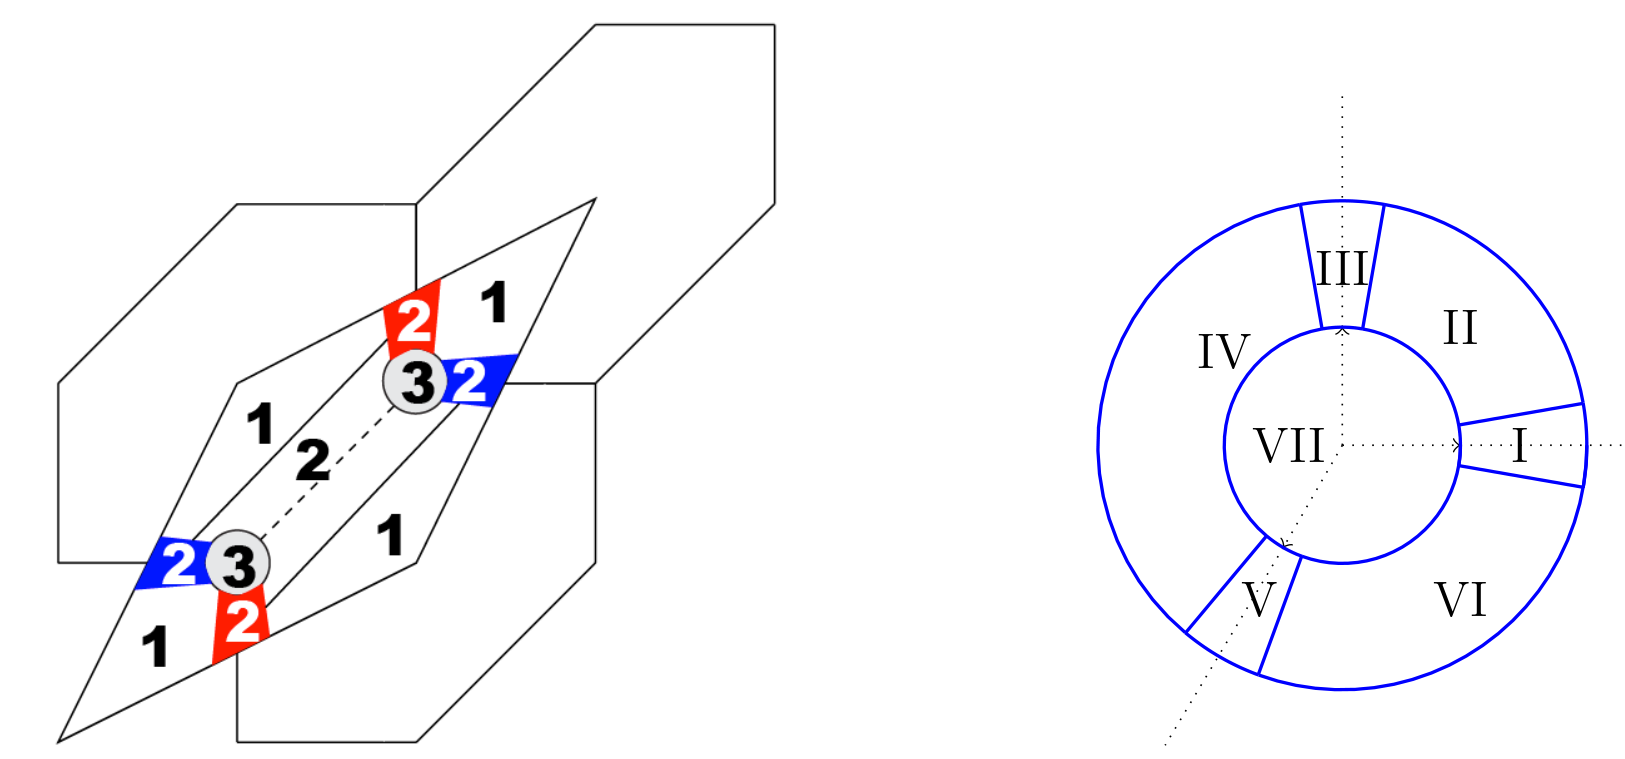
\includegraphics[width=0.86\textwidth]{figures/fig_2_1.png}
\caption{左（L）：所插值的势的数目。右（R）：顶点附近的放大区域。（原书 p.49）}
\label{fig:2-1}
\end{figure}

\medskip
\noindent\textbf{区域 I 的主项}\par
先看没有鼓包函数导数的项。它们应当给出正定矩阵，于是得到度量。随后只需证明：其余各项都能写成（鼓包函数的对数导数）乘（有界项）的形式，而后者只要把 $l$ 取够大就能任意小。首先回忆极坐标下的度量是
\[
\begin{pmatrix}
\partial^2_{r_x}F+\frac{1}{r_x}\partial_{r_x}F & \partial^2_{r_xr_y}F & \partial^2_{r_xr_z}F\\
\partial^2_{r_xr_y}F & \partial^2_{r_y}F+\frac{1}{r_y}\partial_{r_y}F & \partial^2_{r_yr_z}F\\
\partial^2_{r_xr_z}F & \partial^2_{r_yr_z}F & \partial^2_{r_z}F+\frac{1}{r_z}\partial_{r_z}F
\end{pmatrix}.
\]

% ===== 原书 p.50 =====
\begin{gather*}
F=f+\alpha_3d+\alpha_4\cdot\alpha_5\theta,\\
d\approx T^2\Big[r_x^2-\tfrac12(r_y^2+r_z^2)\Big],\\
\theta\approx T^2[r_y^2-r_z^2],\\
f\approx T^2[r_y^2+r_z^2].
\end{gather*}

注意 $r_x$ 处处以 $r_x^2$ 的形式出现，所以作用 $\partial^2_{r_xr_x}$ 等同于作用 $\partial_{r_x}/r_x$。下面列出不含 $\alpha_i$ 导数的项；为记号简便，下标 $x$ 表示 $\partial_{r_x}$：
\[
\begin{aligned}
&\begin{pmatrix}
2(f_{xx}+\alpha_3d_{xx}+\alpha_4\alpha_5\theta_{xx}) & f_{xy}+\alpha_3d_{xy}+\alpha_4\alpha_5\theta_{xy} & f_{xz}+\alpha_3d_{xz}+\alpha_4\alpha_5\theta_{xz}\\
\text{“} & 2(f_{yy}+\alpha_3d_{yy}+\alpha_4\alpha_5\theta_{yy}) & f_{yz}+\alpha_3d_{yz}+\alpha_4\alpha_5\theta_{yz}\\
\text{“} & \text{“} & 2(f_{zz}+\alpha_3d_{zz}+\alpha_4\alpha_5\theta_{zz})
\end{pmatrix}\\
&\qquad\approx T^2
\begin{pmatrix}
4\alpha_3 & 0 & 0\\
0 & 4-2\alpha_3+4\alpha_4\alpha_5 & 0\\
0 & 0 & 4-2\alpha_3-4\alpha_4\alpha_5
\end{pmatrix}.
\end{aligned}
\]

展开式中高阶项的导数会带 $Tr_*$ 变量，因而可以忽略。只要把区域稍微限制一下，这个矩阵就有下界：每个元素都有下界。鼓包函数到达边界时，确有一个坐标趋于零。不过在 $xy$ 平面里趋于零的是 $z$ 项，$xz$ 平面里同理是 $y$ 项。由于我们从底空间加上一项 $|xyz|^2$，离开零纤维处就有正定性。

\medskip
\noindent\textbf{区域 I 中含鼓包函数导数的项}\par
产生鼓包函数导数的项是 $\alpha_3(d_I)d_I$ 与 $\alpha_4(\theta_I)\alpha_5(d_I)\theta_I$。注意在 $r_x=r_y=r_z$ 附近的区域 I 中，$d$ 关于 $(Tr_x)^2$、$(Tr_y)^2$、$(Tr_z)^2$ 近似线性。

记号约定：本节令 $d\equiv d_I$。我们让求导所沿的变量在 $\{r_x,r_y,r_z\}$ 中变动，并把这组变量记作 $\{r_\star,r_\bullet\}\in\{r_x,r_y,r_z\}$。又，$'^{\log}$ 表示取对数导数 $d\alpha_3/d(\log(d_I))=\alpha_3'\cdot d$。下面的二阶导数计算对 $\alpha_5$ 同样适用；把 $d$ 换成 $\theta$ 后对 $\alpha_4$ 也适用。

% ===== 原书 p.51 =====
\begin{align*}
\frac{d^2\alpha_3}{d(\log d)}&=(\alpha_3'\cdot d)'\cdot d=(\alpha_3''\cdot d+\alpha_3')d\\
\Longrightarrow\quad\alpha_3''\cdot d+\alpha_3'&=\frac{1}{d}\cdot\frac{d^2\alpha_3}{d(\log d)^2}\\
\Longrightarrow\quad\alpha_3''&=\frac{1}{d^2}\left(\frac{d^2\alpha_3}{d(\log d)^2}-\frac{d\alpha_3}{d(\log d)}\right)
\end{align*}
% [Tutor Note: 第一行左端原文作 d^2α3 / d(log d)，按上下文应为 d^2α3 / d(log d)^2；照录不改。]

\transnote{本章的 ${\alpha_i'}^{\log}$ 一律指对数导数 $\alpha_i'\cdot d$（或 $\alpha_i'\cdot\theta$），量级为 $1/l$；而 ${\alpha_i''}^{\log}$ 指二阶对数导数，量级为 $1/l^2$。原书在这两个记号与普通导数之间来回换用，读式子时务必先看是哪种：后面的「小量乘有界量」估计全靠 $1/l$ 与 $1/l^2$ 的差别。}

\medskip
\noindent\textbf{$\alpha_3d$ 的导数}\par
一阶导数：$\frac{1}{r_\star}\partial_{r_\star}(\alpha_3d)$。其中 $\alpha_3'd={\alpha_3'}^{\log}$ 是对数导数，可以取得任意小。

二阶导数：$\alpha_3d$ 的二阶导数涉及 $r_\star\alpha_3'd$ 的一阶导数，其中含前面那样的 $\alpha_3'd$ 项，以及 $r_\star(\partial_\bullet d)(\alpha_3''d+\alpha_3')$ 乘以 $T$ 的幂，即正比于 $T^2r_\star r_\bullet(\alpha_3''d+\alpha_3')$，因为 $d$ 关于 $(Tr_x)^2,(Tr_y)^2,(Tr_z)^2$ 近似线性。于是得到
\[
\frac{T^2r_\star r_\bullet}{d}{\alpha_3''}^{\log}.
\]
把分子分母同除以 $r_x^2$，得
\[
\frac{(r_\star r_\bullet)/(r_x)^2}{1-\frac12\big((r_y/r_x)^2+(r_z/r_x)^2\big)},
\]
分母接近 $1$，分子小或等于 $1$，因为 $r_x\gg r_y,r_z$。于是得到有界量乘小量。因此只要 $l$ 固定且足够大，含 $\alpha_3$ 的导数都给出小项。下面写出计算。

\medskip
\noindent\textbf{$\alpha_3(d)\cdot d$ 的对角项：}\par
\begin{align*}
&d\approx T^2\Big[r_x^2-\frac12(r_y^2+r_z^2)\Big],\qquad
d_{r_\star}\approx\lambda T^2r_\star,\quad d_{r_\star r_\star}\approx\lambda T^2,\quad \lambda\in\{2,-1\},\\
&\Big(\frac{1}{r_\star}\partial_{r_\star}+\partial^2_{r_\star r_\star}\Big)(\alpha_3(d)\cdot d)
=\frac{1}{r_\star}\big(\alpha_3'd_{r_\star}d+\alpha_3(d)\cdot d_{r_\star}\big)\\
&\qquad+\big(\alpha_3''d_{r_\star}^2d+\alpha_3'd_{r_\star r_\star}d+2\alpha_3'(d)d_{r_\star}^2+\alpha_3(d)\cdot d_{r_\star r_\star}\big)\\
&\approx\frac{1}{r_\star}\big(\alpha_3'\lambda T^2r_\star d+\alpha_3(d)\cdot\lambda T^2r_\star\big)\\
&\qquad+\big(\alpha_3''(\lambda T^2r_\star)^2d+\alpha_3'\lambda T^2d+2\alpha_3'(d)(\lambda T^2r_\star)^2+\alpha_3(d)\cdot\lambda T^2\big)\\
&=\lambda T^2\big[\alpha_3'd+\alpha_3+\lambda T^2\alpha_3''r_\star^2\cdot d+\alpha_3'd+2\lambda T^2\alpha_3'r_\star^2+\alpha_3(d)\big]\\
&=2\lambda T^2\big[\alpha_3'\big(d+(\lambda-1)T^2r_\star^2\big)+T^2r_\star^2(\alpha_3''d+\alpha_3')\big]+2\lambda T^2\alpha_3\\
&=2\lambda T^2\Big[{\alpha_3'}^{\log}\Big(1+(\lambda-1)\frac{T^2r_\star^2}{d}\Big)+\frac{T^2r_\star^2}{d}{\alpha_3''}^{\log}\Big]+2\lambda T^2\alpha_3.
\end{align*}

% ===== 原书 p.52 =====
\[
{\alpha_3'}^{\log}\approx\frac{\Delta\alpha_3}{\Delta\log d}\approx\propto\frac{1}{l},
\qquad
{\alpha_3''}^{\log}\approx\propto\frac{1}{l^2}.
\]
\[
\frac{T^2r_\star^2}{d}\approx\frac{T^2r_\star^2}{T^2\big[r_x^2-\frac12(r_y^2+r_z^2)\big]}
=\frac{r_\star^2}{r_x^2-\frac12(r_y^2+r_z^2)}
=\frac{r_\star^2/r_x^2}{1-\frac12\Big(\frac{r_y^2}{r_x^2}+\frac{r_z^2}{r_x^2}\Big)}
\approx 1\ \text{或}\ 0\quad\because r_x\gg r_y,r_z.
\]

\medskip
\noindent\textbf{$\alpha_3(d)\cdot d$ 的非对角项，$\star\ne\bullet$：}\par
\begin{align*}
d_{r_\star r_\bullet}&=0\\
\partial^2_{r_\star r_\bullet}(\alpha_3\cdot d)&=\partial_{r_\star}\big(\alpha_3'd_{r_\bullet}d+\alpha_3(d)\cdot d_{r_\bullet}\big)\\
&=\alpha_3''d_{r_\star}d_{r_\bullet}d+\alpha_3'd_{r_\bullet r_\star}d+2\alpha_3'd_{r_\bullet}d_{r_\star}+\alpha_3\cdot d_{r_\bullet r_\star}\\
&=T^4\lambda\mu r_\star r_\bullet\alpha_3''d+0+2T^4\lambda\mu r_\star r_\bullet\alpha_3'+0,\qquad\lambda,\mu\in\{2,-1\}\\
&=T^4\lambda\mu\frac{r_\star r_\bullet}{d}\,d(\alpha_3''d+\alpha_3'+\alpha_3')\\
&=T^4\lambda\mu\frac{r_\star r_\bullet}{d}\big({\alpha_3''}^{\log}+{\alpha_3'}^{\log}\big)
\end{align*}
% [Tutor Note: 上面倒数第二行多出的因子 d 与末行不相容；照录不改。]
\[
\frac{T^2r_\star r_\bullet}{d}\approx\frac{r_\star r_\bullet/r_x^2}{1-\frac12\big((r_y/r_x)^2+(r_z/r_x)^2\big)}\approx 0\ \text{或}\ 1.
\]

又可以看到，鼓包函数的导数全是对数导数，所有项都被常数乘 $T^2/l$ 界住。

\medskip
\noindent\textbf{$\alpha_4\alpha_5\theta$ 的导数}\par
对 $\alpha_4\alpha_5\theta$，一阶导数项（除以求导所沿的变量后）含 $\alpha_5(\alpha_4'\theta)$，这是 $O(1)$ 项（回忆 $\alpha_5$ 从 $0$ 走到 $1$）乘一个对数导数；还含 $\alpha_4(\alpha_5'\theta)=\alpha_4\big({\alpha_5'}^{\log}\cdot\frac{\theta}{d}\big)$，因为 $\alpha_5$ 是 $d$ 的函数。所以要检查 $\theta/d$ 有界且与 $l$ 无关。除以 $r_x^2$ 后分子是小量、分母接近 $1$。因此这两项都没问题。

一阶导数给出 $r_\star\alpha_5(\alpha_4'\theta)$ 与 $r_\star\alpha_4(\alpha_5'\theta)$。把 $r_\star$ 对 $r_\bullet$ 求导，得到上一段已证为小的项；当 $\bullet\ne\star$ 时得零。于是把它提到前面，只对剩下的表达式求导。注意 $\alpha_4$ 是 $\theta$ 的函数，$\alpha_5$ 是 $d$ 的函数。
\begin{itemize}[leftmargin=2.2em,itemsep=0.25em]
\item $r_\star r_\bullet\alpha_4'\alpha_5'\theta=\dfrac{r_\star r_\bullet}{d}{\alpha_4'}^{\log}{\alpha_5'}^{\log}$。这里乘 $d$ 再除以 $d$，以便凑出 $\alpha_5$ 的对数导数。
\item $r_\star r_\bullet\alpha_5(\alpha_4''\theta+\alpha_4')=\alpha_5\cdot\dfrac{r_\star r_\bullet}{\theta}{\alpha_4''}^{\log}$。其中 $r_\bullet$ 来自 $\partial_\bullet\theta$。特别地，若 $r_\bullet=r_x$ 则得零，因为 $\theta\approx T^2[r_y^2-r_z^2]$，即 $\theta_{r_x}\approx0$。
\end{itemize}

% ===== 原书 p.53 =====
\begin{itemize}[leftmargin=2.2em,itemsep=0.25em]
\item $r_\star r_\bullet\alpha_4(\alpha_5''\theta)=\alpha_4\cdot\dfrac{r_\star r_\bullet}{d}\big({\alpha_5''}^{\log}-{\alpha_5'}^{\log}\big)\cdot\dfrac{\theta}{d}$。
\item $r_\star r_\bullet\alpha_4(\alpha_5')=\dfrac{r_\star r_\bullet}{d}\cdot\alpha_4{\alpha_5'}^{\log}$。
\end{itemize}

上面已看到 $T^2\frac{r_\star r_\bullet}{d}$、从而 $\frac{\theta}{d}$ 有界。于是只剩检验 $T^2\frac{r_\star r_\bullet}{\theta}$ 有界。另外，按上面的说明，分子含 $r_x$ 时得零；又由二阶偏导数对称，只需考虑分子不含 $r_x$ 的情形。因此要估计下列表达式：
\[
\frac{r_y^2}{r_y^2-r_z^2},\qquad
\frac{r_z^2}{r_y^2-r_z^2},\qquad
\frac{r_yr_z}{r_y^2-r_z^2}.
\]

我们看区域 I 的上半部分，那里 $r_y>r_z$。我们规定 $\alpha_4$ 在区域 $1<\left(\frac{r_y}{r_z}\right)^2<\frac1T$ 内取常值。于是 $\alpha_4$ 的支撑集是 $\left(\frac{r_y}{r_z}\right)^2>\frac1T$。特别地，
\[
\frac{1}{\left(\frac{r_y}{r_z}\right)^2-1}<\frac{1}{\frac1T-1}=\frac{T}{1-T}\approx T.
\]
所以这些项有界；把分子分母同除以 $r_z^2$ 即可看出。下面是具体计算。

对角项为 $\frac{1}{r_\bullet}\partial_{r_\bullet}+\partial^2_{r_\bullet r_\bullet}$，非对角项为 $\partial^2_{r_\bullet r_\star}$。
\begin{align*}
\theta&\approx T^2(r_y^2-r_z^2),\\
d&\approx T^2\big(r_x^2-\tfrac12(r_y^2+r_z^2)\big),\\
\theta_{r_\bullet}&\approx\lambda_\bullet T^2r_\bullet,\qquad\lambda_\bullet\in\{0,\pm2\},\\
d_{r_\bullet}&\approx\mu_\bullet T^2r_\bullet,\qquad\mu_\bullet\in\{2,-1\},\\
\frac{1}{r_\bullet}\partial_{r_\bullet}(\alpha_4\alpha_5\theta)
&=\frac{1}{r_\bullet}\big(\alpha_4'\theta_{r_\bullet}\alpha_5\theta+\alpha_4\alpha_5'd_{r_\bullet}\theta+\alpha_4\alpha_5\theta_{r_\bullet}\big)\\
&=T^2\Big(\lambda_\bullet{\alpha_4'}^{\log}\alpha_5+\mu_\bullet\alpha_4{\alpha_5'}^{\log}\frac{\theta}{d}+\lambda_\bullet\alpha_4\alpha_5\Big).
\end{align*}

% ===== 原书 p.54 =====
\begin{align*}
\partial^2_{r_\star r_\bullet}(\alpha_4\alpha_5\theta)
&=T^2\partial_{r_\star}\big[r_\bullet\lambda_\bullet\alpha_4'\theta\alpha_5+r_\bullet\mu_\bullet\alpha_4\alpha_5'\theta+r_\bullet\lambda_\bullet\alpha_4\alpha_5\big]\\
&=T^2\big[\partial_{r_\star}r_\bullet\lambda_\bullet\alpha_4'\theta\alpha_5
+T^2r_\bullet\lambda_\bullet\alpha_4''\theta_{r_\star}\theta\alpha_5\\
&\qquad+T^2r_\bullet\lambda_\bullet\alpha_4'\theta_{r_\star}\alpha_5
+T^2r_\bullet\lambda_\bullet\alpha_4'\theta\alpha_5'd_{r_\star}
+\partial_{r_\star}(r_\bullet)\alpha_4\alpha_5'\theta\\
&\qquad+T^2r_\bullet\mu_\bullet\alpha_4'\theta_{r_\star}\alpha_5'\theta
+T^2r_\bullet\mu_\bullet\alpha_4\alpha_5''d_{r_\star}\theta
+T^2r_\bullet\mu_\bullet\alpha_4\alpha_5'\theta_{r_\star}\\
&\qquad+\partial_{r_\star}(r_\bullet)\lambda_\bullet\alpha_4\alpha_5
+T^2r_\bullet\lambda_\bullet\alpha_4'\theta_{r_\star}\alpha_5
+T^2r_\bullet\lambda_\bullet\alpha_4\alpha_5'd_{r_\star}\big]\\
&=T^2\Big[\delta_{\bullet\star}\lambda_\bullet{\alpha_4'}^{\log}\alpha_5
+T^2\Big[\lambda_\bullet\lambda_\star\frac{r_\bullet r_\star}{\theta}\big({\alpha_4''}^{\log}-{\alpha_4'}^{\log}\big)\alpha_5\\
&\qquad+\lambda_\bullet\lambda_\star\frac{r_\bullet r_\star}{\theta}{\alpha_4'}^{\log}\alpha_5
+\lambda_\bullet\mu_\star\frac{r_\bullet r_\star}{d}{\alpha_4'}^{\log}{\alpha_5'}^{\log}\Big]\\
&\qquad+\delta_{\star\bullet}\frac{\theta}{d}\alpha_4{\alpha_5'}^{\log}
+\mu_\bullet\lambda_\star\frac{T^2r_\bullet r_\star}{d}{\alpha_4'}^{\log}{\alpha_5'}^{\log}\\
&\qquad+\frac{T^2r_\bullet r_\star\theta}{d^2}\alpha_4\big({\alpha_5''}^{\log}-{\alpha_5'}^{\log}\big)
+\mu_\bullet\lambda_\star\frac{T^2r_\bullet r_\star}{d}{\alpha_5'}^{\log}\\
&\qquad+\delta_{\star\bullet}\lambda_\bullet\alpha_4\alpha_5
+\lambda_\bullet\lambda_\star\frac{T^2r_\bullet r_\star}{\theta}{\alpha_4'}^{\log}\alpha_5
+\lambda_\bullet\mu_\star\frac{T^2r_\bullet r_\star}{d}\alpha_4{\alpha_5'}^{\log}\Big].
\end{align*}

我们看到 $T^2\frac{r_\bullet r_\star}{\theta}$、$T^2\frac{r_\bullet r_\star}{d}$、$\frac{\theta}{d}$ 如上都有界，且其中的导数都是对数导数。

\medskip
\noindent\textbf{把区域 III 与 V 调成与区域 I 一致}\par
区域 I 中 $r_x$ 是主导坐标。区域 III 中 $r_y$ 将主导，区域 V 中 $r_z$ 将主导。于是仿照 I，取 III 与 V 各半区域的相应数据。

\begin{figure}[htbp]
\centering
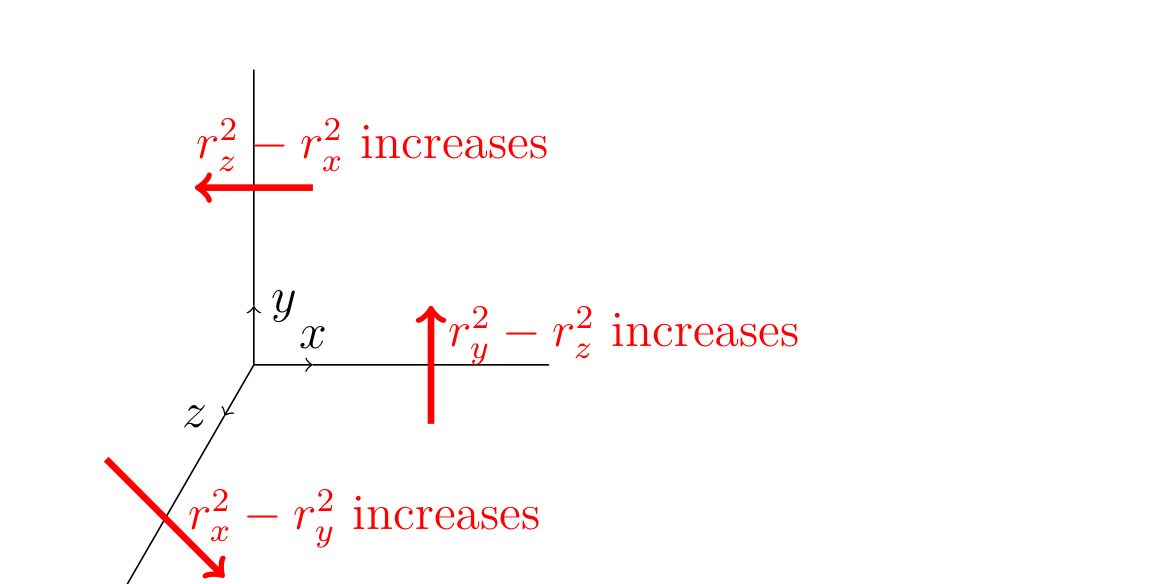
\includegraphics[width=0.62\textwidth]{figures/fig_2_2.png}
\caption{三个角方向。（原书 p.54）}
\label{fig:2-2}
\end{figure}

\begin{gather*}
g_{yz}=g_{yz}+\alpha_3(d_I)\cdot d_I+\alpha_4(\theta_I)\alpha_5(d_I)\cdot\theta_I\\
g_{yz}\approx T^2[r_y^2+r_z^2]\\
\theta_I\approx T^2[r_y^2-r_z^2]\\
d_I\approx T^2\Big[r_x^2-\frac12(r_y^2+r_z^2)\Big]
\end{gather*}
% [Tutor Note: 第一行左端原文写作 g_yz = g_yz + …，按上下文应为 F = g_yz + …；照录不改。]

% ===== 原书 p.55 =====
\begin{gather*}
g_{xy}=g_{xy}+\alpha_3(d_{III})\cdot d_{III}+\alpha_4(\theta_{III})\alpha_5(d_{III})\cdot\theta_{III}\\
g_{xy}\approx T^2[r_x^2+r_z^2]\\
\theta_{III}\approx T^2[r_z^2-r_x^2]\\
d_{III}\approx T^2\Big[r_y^2-\frac12(r_x^2+r_z^2)\Big]
\end{gather*}
\begin{gather*}
F_V=f_V+\alpha_3(d_V)\cdot d_V+\alpha_4(\theta_V)\alpha_5(d_V)\cdot\theta_V\\
f_V\approx T^2[r_x^2+r_y^2]\\
\theta_V\approx T^2[r_x^2-r_y^2]\\
d_V\approx T^2\Big[r_z^2-\frac12(r_x^2+r_y^2)\Big]
\end{gather*}

已知起点是 $\alpha_1g_{xy}+\alpha_2g_{xz}+(1-\alpha_1-\alpha_2)g_{yz}$，而终点应是 III 与 V 中的上述表达式；由于角方向与径向方向按上面的对称性确定，这就定下了 III 与 V 中 $\alpha_3$ 与 $\alpha_4\cdot\alpha_5$ 的取值。

区域 III 中要求
\begin{align*}
F&=g_{xy}+\alpha_3(d_{III})\cdot d_{III}+\alpha_4(\theta_{III})\alpha_5(d_{III})\cdot\theta_{III}\\
&=g_{xz}+\alpha_3\Big(\frac12(g_{yz}-g_{xz})+\frac12(g_{xy}-g_{xz})\Big)+\alpha_4\alpha_5(g_{yz}-g_{xy})\\
&=g_{xz}(1-\alpha_3)+g_{xy}\Big(\frac{\alpha_3}{2}-\alpha_4\alpha_5\Big)+g_{yz}\Big(\frac{\alpha_3}{2}+\alpha_4\alpha_5\Big)\\
&=\alpha_1g_{xy}+\alpha_2g_{xz}+(1-\alpha_1-\alpha_2)g_{yz}\\
&\Longrightarrow\quad\alpha_3=1-\alpha_2,\qquad\alpha_4\cdot\alpha_5=\frac12-\frac{\alpha_2}{2}-\alpha_1.
\end{align*}
% [Tutor Note: 上面第一行左端的 g_xy 与第二行的 g_xz 不一致；按 d_III 的展开，基项应为 g_xz。照录不改。]

区域 V 中要求
\begin{align*}
F&=f_V+\alpha_3(d_V)\cdot d_V+\alpha_4(\theta_V)\alpha_5(d_V)\cdot\theta_V\\
&=g_{xy}+\alpha_3\Big(\frac12(g_{xz}-g_{xy})+\frac12(g_{yz}-g_{xy})\Big)+\alpha_4\alpha_5(g_{xz}-g_{yz})\\
&=g_{xy}(1-\alpha_3)+g_{xz}\Big(\frac{\alpha_3}{2}+\alpha_4\alpha_5\Big)+g_{yz}\Big(\frac{\alpha_3}{2}-\alpha_4\alpha_5\Big)\\
&=\alpha_1g_{xy}+\alpha_2g_{xz}+(1-\alpha_1-\alpha_2)g_{yz}\\
&\Longrightarrow\quad\alpha_3=1-\alpha_1,\qquad\alpha_4\cdot\alpha_5=\alpha_2-\frac12+\frac{\alpha_1}{2}.
\end{align*}

% ===== 原书 p.56 =====
两种情形中 $\alpha_3$ 都从 $2/3$ 走到 $1$，$\alpha_4$ 都从 $-1/2$ 走到 $1/2$，$\alpha_5$ 则从 $0$ 到 $1$ 给它作缩放。既然一切都在 $(r_x,r_y,r_z)$ 下对称，前面的计算对 $f+\alpha_3d+\alpha_4\alpha_5\theta$ 照旧成立。现在的问题在于：$\alpha_{\ge3}$ 是 $d$ 与 $\theta$ 的函数，而这两个变量在三个区域中各有不同定义。因此我们要把 $d$ 坐标沿区域 II、IV、VI 拼接起来。

之所以只需拼接 $d$，是因为在奇数区域边界处 $\alpha_4$ 已经变平到 $1/2$ 或 $-1/2$，而 $\alpha_3,\alpha_5$ 只依赖 $d$。于是再取一个从 $0$ 到 $1$ 的鼓包函数 $\alpha_6$，在偶数区域里加入越来越多的 $\theta$ 坐标，从而在 $d$ 的两种定义之间插值。归纳一下：在 II、IV、VI 中，$\alpha_3$ 与 $\alpha_5$ 是 $d$ 的函数，而 $d$ 又是 $\alpha_6(\theta_{\text{even}})\cdot\theta_{\text{even}}$ 的函数。于是对 $r_x,r_y,r_z$ 求导时，链式法则要用两层。

\medskip
\noindent\textbf{区域 IIA 的主项}\par
先取不含鼓包函数导数的项。它们构成区域 II 上度量的非退化部分；其余各项我们会证明可以取得足够小。因为一切非鼓包的量都关于 $(Tr_x)^2$、$(Tr_y)^2$、$(Tr_z)^2$ 近似线性，所以仍有 $\frac{1}{r_x}\partial_{r_x}=\partial^2_{r_xr_x}$。回忆 $2/3\le\alpha_3\le1$，$0\le\alpha_5,\alpha_6\le1$。先修正第一行中的 $\phi$ 项。
\transnote{原文此处夹有作者的工作批注「Fix $\phi$ terms in first line.」，语义不明；照录为「先修正第一行中的 $\phi$ 项」。}

\begin{align*}
F&\approx T^2\Big[\big(r_y^2+r_z^2-\alpha_6(\theta_{II})\cdot r_y^2\big)
+\alpha_3(d_{IIA})\cdot\Big(r_x^2-\frac12(r_y^2+r_z^2)+\frac32\alpha_6(\theta_{II})\cdot r_y^2\Big)\\
&\qquad+\frac12\alpha_5(d_{IIA})\cdot\big(r_y^2-r_z^2-\alpha_6(\theta_{II})\cdot r_y^2\big)\Big]
\end{align*}

非对角项 $\partial^2_{r_\bullet r_\star}$（$\star\ne\bullet$）为零，因为对非鼓包函数求导就是对某个 $r_*^2$ 求导。对角项有 $\frac{1}{r_*}\partial_{r_*}+\partial^2_{r_*r_*}=2\partial^2_{r_*r_*}$，作用在 $(Tr_*)^2$ 上得 $2T^2$。于是矩阵的 $(*,*)$ 元中，主项是 $4T^2$ 乘 $r_*^2$ 的系数。$y$ 那一项还要核对。
\begin{align*}
x:\quad &T^2(4\alpha_3)\ge T^2\frac83,\\
y:\quad &T^2(4-4\alpha_6-2\alpha_3+6\alpha_3\alpha_6+2\alpha_5-2\alpha_5\alpha_6)
=T^2\big[4+(2-2\alpha_6)(\alpha_5-\alpha_3)+4\alpha_6(\alpha_3-1)\big]\\
&\ge T^2\big[4+2(0-2/3)+4(-1/3)\big]=T^2\cdot\frac43,\\
z:\quad &T^2(4-2\alpha_3-2\alpha_5).
\end{align*}

注意当 $\alpha_3=\alpha_5=1$ 时 $z$ 项趋于零。不过在 $\alpha_3,\alpha_5$ 与 $1$ 保持距离的区域里它有下界。在它趋于 $1$ 的区域，我们从底空间给 $F$ 加上一项 $|xyz|^2$，以维持非退化性。由于在加这一项的区域里 $xyz$ 有正的下界，求偏导数后得到的仍是正定的。

% ===== 原书 p.57 =====
\medskip
\noindent\textbf{区域 IIA 中含鼓包函数导数的项}\par
下面证明含鼓包函数导数的项可以取得很小。备查：
\begin{gather*}
F\approx\big(g_{yz}-\alpha_6\cdot(Tr_y)^2\big)+\alpha_3(d_{IIA})d_{IIA}
+\frac12\alpha_5(d_{IIA})\cdot\big((Tr_y)^2-(Tr_z)^2-\alpha_6(Tr_y)^2\big)\\
g_{yz}\approx T^2[r_y^2+r_z^2]\\
d_I\approx T^2\Big[r_x^2-\frac12(r_y^2+r_z^2)\Big]\\
d_{IIA}\approx T^2\Big[r_x^2-\frac12(r_y^2+r_z^2)\Big]+\frac32\alpha_6(\log r_y-\log r_x)\cdot(Tr_y)^2\\
\theta_I\approx T^2[r_y^2-r_z^2]\\
\theta_{II}=\log(r_y/r_x)
\end{gather*}

$F$ 中的鼓包函数项是：$\alpha_6\cdot(Tr_y)^2$、$\alpha_3\cdot d_{IIA}$、$\{\alpha_5(Tr_*)^2\}_{*=y,z}$、$\alpha_5\alpha_6\cdot(Tr_y)^2$。

第 1 项：$\alpha_6(\log(r_y/r_x))\cdot(Tr_y)^2$。

\medskip
\noindent 一阶导数（除以 $r_\star$）：
\begin{align*}
\frac{1}{r_x}\partial_{r_x}\big[\alpha_6(\log r_y-\log r_x)(Tr_y)^2\big]
&=-\frac{1}{r_x^2}\alpha_6'\cdot(Tr_y)^2=-T^2\cdot\frac{r_y^2}{r_x^2}\alpha_6',
\qquad\Big|\frac{r_y^2}{r_x^2}\Big|<1\\
\frac{1}{r_y}\partial_{r_y}\big[\alpha_6(\log r_y-\log r_x)(Tr_y)^2\big]
&=\frac{1}{r_y^2}\alpha_6'\cdot(Tr_y)^2+\alpha_6\cdot(2T^2r_y)=T^2\alpha_6'+2T^2\alpha_6r_y\\
\frac{1}{r_z}\partial_{r_z}\big[\alpha_6(\log r_y-\log r_x)(Tr_y)^2\big]&=0\\
\alpha_6'&\approx\propto\frac1l
\end{align*}

于是这一项的一阶导数给出的鼓包函数导数项都能取得很小。

\medskip
\noindent 二阶导数 $\partial^2_\bullet$：
\begin{align*}
\partial^2_{r_xr_x}(\alpha_6(Tr_y)^2)&=\partial_{r_x}\Big(-\frac{(Tr_y)^2}{r_x}\alpha_6'\Big)
=\frac{(Tr_y)^2}{r_x^2}(\alpha_6'+\alpha_6'')\\
&<T^2(\alpha_6'+\alpha_6'')\approx\propto T^2\Big(\frac1l+\frac1{l^2}\Big),\ \text{小}\\
\partial^2_{r_xr_y}(\alpha_6(Tr_y)^2)&=\partial_{r_y}\Big(-\frac{(Tr_y)^2}{r_x}\alpha_6'\Big)
=\frac{-T^2r_y}{r_x}(2\alpha_6'+\alpha_6''),\\
&\qquad\text{范数}<T^2(2\alpha_6'+\alpha_6'')\\
\partial^2_{r_yr_y}(\alpha_6(Tr_y)^2)&=\partial_{r_y}\big(T^2\alpha_6'r_y+2T^2\alpha_6r_y^2\big)\\
&=T^2(\alpha_6'+\alpha_6''+2\alpha_6'r_y+4\alpha_6r_y)<T^2(3\alpha_6'+\alpha_6''+4\alpha_6r_y)
\end{align*}

因为区域 II 中 $r_y$ 很小。注意一阶导数 $\alpha_6'$ 从 $0$ 增到 $l/2$ 中点处的最大值 $1/l+\epsilon$，因此斜率的变化约为 $1/l^2$，仍然很小。（确切地说是 $(1/l+\epsilon)(2/l)$。）所以 $\alpha_6r_y^2$ 这一项没有问题。

第 2 项：$\alpha_3(d_{IIA})d_{IIA}$。

% ===== 原书 p.58 =====
\medskip
\noindent\textbf{一阶导数。}$\frac{1}{r_\star}\partial_{r_\star}(\alpha_3d_{IIA})=(\alpha_3'd_{IIA}+\alpha_3)\cdot\frac{d_{IIA,\star}}{r_\star}$。下面是 $d_{IIA}$ 的偏导数。
\begin{align*}
d_{IIA}&\approx T^2\Big[r_x^2-\frac12(r_y^2+r_z^2)\Big]+\frac32\alpha_6(\log r_y-\log r_x)\cdot(Tr_y)^2\\
\frac{(d_{IIA})_x}{r_x}&=\frac{T^2}{r_x}\Big[2r_x+\frac32\Big(\alpha_6'\cdot\frac{-1}{r_x}\cdot r_y^2\Big)\Big]
=T^2\Big[2+\frac32\Big(\alpha_6'\cdot\frac{-r_y^2}{r_x^2}\Big)\Big]\\
\frac{(d_{IIA})_y}{r_y}&=\frac{T^2}{r_y}\Big[-r_y+\frac32\Big(\alpha_6'\cdot\frac1{r_y}\cdot r_y^2+2r_y\alpha_6\Big)\Big]
=T^2\Big[-1+\frac32(\alpha_6'+2\alpha_6)\Big]\\
\frac{(d_{IIA})_z}{r_z}&=\frac{T^2}{r_z}[-r_z]=-T^2
\end{align*}

于是 $\frac{1}{r_\star}\partial_{r_\star}(\alpha_3d_{IIA})=(\alpha_3'd_{IIA}+\alpha_3)\cdot\frac{d_{IIA,\star}}{r_\star}$ 中的项如下：
\begin{itemize}[leftmargin=2.2em,itemsep=0.2em]
\item 用 $\frac{d_{IIA,\star}}{r_\star}$ 中可能出现的项乘 $\alpha_3'd_{IIA}$：
 \begin{itemize}[leftmargin=1.8em,itemsep=0.15em]
 \item $\alpha_3'd_{IIA}$：$\star$ 任意，来自各个 $\frac{d_{IIA,\star}}{r_\star}$ 的常数项；
 \item $\alpha_3'd_{IIA}\alpha_6$：$\star=y$，因为 $\alpha_6$ 只出现在 $\star=y$ 的导数里；
 \item $\alpha_3'd_{IIA}\alpha_6'$：$\star=y$，同上；
 \item $\alpha_3'd_{IIA}\alpha_6'\cdot\left(\frac{r_y}{r_x}\right)^2$：仅 $\star=x$。
 \end{itemize}
\item 用 $\frac{d_{IIA,\star}}{r_\star}$ 乘 $\alpha_3$：
 \begin{itemize}[leftmargin=1.8em,itemsep=0.15em]
 \item $\alpha_3$：$\star$ 任意；
 \item $\alpha_3\alpha_6$：$\star=y$；
 \item $\alpha_3\alpha_6'$：$\star=y$；
 \item $\alpha_3\alpha_6'\cdot\left(\frac{r_y}{r_x}\right)^2$：$\star=x$。
 \end{itemize}
\end{itemize}

这里每一项都没问题：要么得到 ${\alpha_3'}^{\log}=\alpha_3'd_{IIA}$，要么得到 $\alpha_6$ 的通常导数；后者可能乘上 $(r_y/r_x)^2$，而区域 IIA 中 $r_x>r_y$，所以导数项可以取得很小。

\medskip
\noindent\textbf{二阶导数项。} 对上列每个一阶导数项求导。设 $P$ 是上表中的一项。因为前面除以了 $r_\star$，现在要对 $r_\star P$ 求导。用微分算子 $D=\partial_{r_\bullet}$ 与乘积法则得 $D(r_\star)P+r_\star D(P)$。第一项给出 $0$ 或 $1$ 乘 $P$，而上表已说明每个 $P$ 都小。所以只需对上表 8 种 $P$ 考察 $r_\star D(P)$。

\transnote{这里把二阶导数的检验压缩成「只需看 $r_\star D(P)$」，理由是 $D(r_\star)$ 只给出 $0$ 或 $1$，而 $1$ 倍的那部分已知是小量。抓这一点是本段长清单的目的：$P$ 一共 8 种，若逐一从头算二阶导数会失控，先剥掉 $D(r_\star)P$ 才把工作量化到 8 个小计算。}

% ===== 原书 p.59 =====
\medskip
\noindent\textbf{1.}\ $P=\alpha_3'd_{IIA}$。

这一项通过 $r_\star\partial_{r_\bullet}(P)$ 给 $\partial^2_{r_\star r_\bullet}(F)$ 作贡献，即
\[
r_\star\partial_{r_\bullet}(\alpha_3'd_{IIA})
=r_\star\alpha_3''\cdot(d_{IIA})_\bullet\cdot d_{IIA}+r_\star\alpha_3'(d_{IIA})_\bullet
=\frac{r_\star(d_{IIA})_\bullet}{d_{IIA}}{\alpha_3''}^{\log},
\]
\[
(d_{IIA})_\bullet\ \text{的取值}:\ \Big\{T^2r_\bullet,\ T^2\alpha_6r_y,\ T^2\alpha_6'r_y,\ T^2\alpha_6'\frac{r_y^2}{r_x}\Big\}<T^2r_\bullet,
\quad\because\alpha_6\le1,\ \alpha_6'\approx\propto\frac1l,\ \frac{r_y}{r_x}<1,
\]
\[
\begin{aligned}
\frac{T^2r_\star r_\bullet}{d_{IIA}}
&\approx\frac{r_\star r_\bullet}{r_x^2-\frac12(r_y^2+r_z^2)+\frac32\alpha_6r_y^2}
=\frac{r_\star r_\bullet/r_x^2}{1-\frac12\big((r_y/r_x)^2+(r_z/r_x)^2\big)+\frac32\alpha_6(r_y/r_x)^2}\\
&\approx\frac{r_\star r_\bullet}{r_x^2}\in\{0,1\}
\quad\because r_x\gg r_y,r_z\ \text{在区域 IIA}.
\end{aligned}
\]
\[
\therefore\quad r_\star\partial_{r_\bullet}(P)=\frac{r_\star(d_{IIA})_\bullet}{d_{IIA}}{\alpha_3''}^{\log}\approx(\text{有界})\cdot\frac1{l^2}.
\]

\medskip
\noindent\textbf{2.}\ $P=\alpha_3'd_{IIA}\alpha_6$，来自对 $F$ 先按 $y$ 求导，即 $\partial_{r_y}(F)$。
\begin{align*}
r_y\partial_{r_\bullet}(\alpha_3'd_{IIA}\alpha_6)
&=r_y\partial_{r_\bullet}(\alpha_3'd_{IIA})\cdot\alpha_6+r_y(\alpha_3'd_{IIA})\cdot\partial_{r_\bullet}(\alpha_6)\\
&=(\text{上一情形})\cdot\alpha_6\pm{\alpha_3'}^{\log}\alpha_6'\cdot cr_y,\qquad c\in\Big\{\frac1{r_x},\frac1{r_y},0\Big\}\\
&=\text{小}+\text{小}.
\end{align*}

\medskip
\noindent\textbf{3.}\ $\alpha_3'd_{IIA}\alpha_6'$，来自先按 $y$ 求导。与第 2 条相同，把 $\alpha_6$ 换成 $\alpha_6'$。

\medskip
\noindent\textbf{4.}\ $\alpha_3'd_{IIA}\alpha_6'\cdot\left(\frac{r_y}{r_x}\right)^2$，来自先按 $x$ 求导。
\begin{align*}
r_x\partial_{r_\bullet}\Big(\alpha_3'd_{IIA}\alpha_6'\cdot\Big(\frac{r_y}{r_x}\Big)^2\Big)
&=r_x\partial_{r_\bullet}(\alpha_3'd_{IIA}\alpha_6')\cdot\Big(\frac{r_y}{r_x}\Big)^2
+r_x(\alpha_3'd_{IIA}\alpha_6')\cdot\partial_{r_\bullet}\Big(\Big(\frac{r_y}{r_x}\Big)^2\Big)\\
&=\frac{r_y}{r_x}\cdot r_y\partial_{r_\bullet}(\alpha_3'd_{IIA}\alpha_6')
\pm({\alpha_3'}^{\log}\alpha_6')\cdot cr_x,\qquad c\in\Big\{\frac{2r_y^2}{r_x^3},\frac{2r_y}{r_x^2},0\Big\}\\
&=(\text{小})(\text{上一情形})+(\text{小})\Big(\frac{r_y}{r_x}\Big)^i,\qquad i\in\{1,2\}\\
&=\text{小}\quad\because r_x\gg r_y.
\end{align*}

\medskip
\noindent\textbf{5.}\ $P=\alpha_3$：它出现在 $F$ 对任一变量的一阶导数中。

再求一次导得 $r_\star\partial_{r_\bullet}\alpha_3=r_\star\alpha_3'(d_{IIA})_\bullet={\alpha_3'}^{\log}\cdot(r_\star(d_{IIA})_\bullet)/d_{IIA}$。所以要 $(r_\star(d_{IIA})_\bullet)/d_{IIA}$ 有界；第 1 条已检验过。

\medskip
\noindent\textbf{6.}\ $P=\alpha_3\alpha_6$：它出现在 $F$ 对 $y$ 的一阶导数中。
\[
r_y\partial_{r_\bullet}(\alpha_3\alpha_6)=r_y\big((\alpha_3)_\bullet\alpha_6+\alpha_3(\alpha_6)_\bullet\big).
\]

% ===== 原书 p.60 =====
含 $\alpha_3$ 导数的那项已归入上一情形。第二项给出 $\alpha_3\alpha_6'$ 乘 $\{0,\ r_y/r_x\approx0,\ 1\}$ 之一，于是这一项是有界量乘小量，同样小。

\medskip
\noindent\textbf{7.}\ $P=\alpha_3\alpha_6'$：$\star=y$。把上一情形中的 $\alpha_6$ 换成 $\alpha_6'$。

\medskip
\noindent\textbf{8.}\ $P=\alpha_3\alpha_6'(r_y/r_x)^2$：$\star=x$。计算与第 4 条完全相同，只是「已检验」的部分现在是 $\alpha_3\alpha_6'$ 而不是 $\alpha_3'd_{IIA}\alpha_6'$。

至此完成了 $\alpha_3(d_{IIA})d_{IIA}$ 一阶与二阶导数的检验。

\[
\text{第 3 项：}\ \alpha_5\cdot(Tr_*)^2,\qquad *\in\{y,z\}
\]

我们照搬上面 $\alpha_3\cdot d_{IIA}$ 的论证，只把第二项里的 $d_{IIA}$ 换成 $(Tr_*)^2$。

\medskip
\noindent\textbf{一阶导数。}$\frac{1}{r_\star}\partial_{r_\star}(\alpha_5(Tr_*)^2)=\frac{1}{r_\star}\alpha_5'(d_{IIA})_\star(Tr_*)^2+\alpha_5\cdot\frac{((Tr_*)^2)_\star}{r_\star}$。而 $(Tr_*)^2$ 的偏导数是 $\frac{1}{r_\star}\partial_{r_\star}((Tr_*)^2)=2T^2$ 或 $0$。

于是 $\frac{1}{r_\star}\partial_{r_\star}(\alpha_5(Tr_*)^2)$ 中的非零项是 $2T^2\alpha_5$ 与
\[
\frac{1}{r_\star}\alpha_5'(d_{IIA})_\star(Tr_*)^2={\alpha_5'}^{\log}\frac{T^2r_*^2(d_{IIA})_\star}{d_{IIA}r_\star}.
\]
注意 $\frac{T^2r_*^2}{d_{IIA}}$ 与 $\frac{(d_{IIA})_\star}{r_\star}$ 都有界；后者已在第 2、3 条中检验。前者：
\[
\frac{r_*^2}{r_x^2-\frac12(r_y^2+r_z^2)+\frac32\alpha_6r_y^2}
=\frac{r_*^2/r_x^2}{1-\frac12\big((r_y/r_x)^2+(r_z/r_x)^2\big)+\frac32\alpha_6(r_y/r_x)^2}
\approx0\quad\because r_x\gg r_y,r_z.
\]
注意 $*\in\{y,z\}$。所以一阶导数没问题：要么是非鼓包函数的导数，要么是有界量乘小对数导数。

\medskip
\noindent\textbf{二阶导数项。} 逐个对一阶导数项求导。它们是 $\alpha_5'(d_{IIA})_*(Tr_*)^2$ 与 $2T^2r_*\alpha_5$。设 $Pr_*$ 是其中一项，即上一条中考虑的 $P$。用微分算子 $D=\partial_{r_\bullet}$ 与乘积法则得 $D(r_*)P+r_*D(P)$。第一项给出 $0$ 或 $1$ 乘 $P$，上面已说明每个 $P$ 都小。所以只需对这 2 种 $P$ 考察 $r_*D(P)$。

\medskip
\noindent\textbf{1.}\ $P=\alpha_5'(Tr_*)^2\frac{(d_{IIA})_*}{r_*}$。这涉及下面的项：把 $\alpha_5'(Tr_*)^2$ 乘上 $\frac{(d_{IIA})_*}{r_*}$ 中出现的四类项，再逐类检验由此产生的二阶导数。

% ===== 原书 p.61 =====
\medskip
\noindent（i）$\alpha_5'(Tr_*)^2$：这一项通过 $r_\star\partial_{r_\bullet}(P)$ 给 $\partial^2_{r_\star r_\bullet}(F)$ 作贡献，即
\begin{align*}
r_\star\partial_{r_\bullet}(\alpha_5'(Tr_*)^2)
&=r_\star\alpha_5''\cdot(d_{IIA})_\bullet\cdot(Tr_*)^2+r_\star\alpha_5'((Tr_*)^2)_\bullet\\
&=\big({\alpha_5''}^{\log}-{\alpha_5'}^{\log}\big)\frac{r_\star(d_{IIA})_\bullet(Tr_*)^2}{d_{IIA}^2}
+{\alpha_5'}^{\log}\frac{2T^2r_\bullet r_\star}{d_{IIA}}.
\end{align*}
已检验有界：$\frac{r_\star(d_{IIA})_\bullet}{d_{IIA}}$（第 1 条）、$\frac{(Tr_*)^2}{d_{IIA}}$（上面）、$\frac{T^2r_\bullet r_\star}{d_{IIA}}$（第 1 条）。因此
\[
\therefore\quad r_\star\partial_{r_\bullet}(\alpha_5'(Tr_*)^2)=(\text{小})(\text{有界})+(\text{小})(\text{有界}).
\]

\medskip
\noindent（ii）$\alpha_5'(Tr_*)^2\alpha_6$：来自对 $F$ 先按 $y$ 求导，即 $\partial_{r_y}(F)$。
\begin{align*}
r_y\partial_{r_\bullet}(\alpha_5'(Tr_*)^2\alpha_6)
&=r_y\partial_{r_\bullet}(\alpha_5'(Tr_*)^2)\cdot\alpha_6+r_y(\alpha_5'(Tr_*)^2)\cdot\partial_{r_\bullet}(\alpha_6)\\
&=(\text{上一情形})\cdot\alpha_6\pm{\alpha_5'}^{\log}\frac{(Tr_*)^2}{d_{IIA}}\alpha_6'\cdot cr_y,
\qquad c\in\Big\{\frac1{r_x},\frac1{r_y},0\Big\}\\
&=(\text{小})(\text{有界})+(\text{小})(\text{有界}).
\end{align*}

\medskip
\noindent（iii）$\alpha_5'(Tr_*)^2\alpha_6'$：来自先按 $y$ 求导。与上一情形相同，把 $\alpha_6$ 换成 $\alpha_6'$。

\medskip
\noindent（iv）$\alpha_5'(Tr_*)^2\alpha_6'\cdot\left(\frac{r_y}{r_x}\right)^2$：来自先按 $x$ 求导。
\begin{align*}
r_x&\partial_{r_\bullet}\Big(\alpha_5'(Tr_*)^2\alpha_6'\Big(\frac{r_y}{r_x}\Big)^2\Big)\\
&=r_x\partial_{r_\bullet}(\alpha_5'(Tr_*)^2\alpha_6')\cdot\Big(\frac{r_y}{r_x}\Big)^2
+r_x(\alpha_5'(Tr_*)^2\alpha_6')\cdot\partial_{r_\bullet}\Big(\Big(\frac{r_y}{r_x}\Big)^2\Big)\\
&=\frac{r_y}{r_x}\cdot r_y\partial_{r_\bullet}(\alpha_5'(Tr_*)^2\alpha_6')\\
&\qquad\pm\Big({\alpha_5'}^{\log}\frac{(Tr_*)^2}{d_{IIA}}\alpha_6'\Big)\cdot cr_x,
\qquad c\in\Big\{\frac{2r_y^2}{r_x^3},\frac{2r_y}{r_x^2},0\Big\}\\
&=(\text{小})(\text{上一情形})+(\text{小})\Big(\frac{r_y}{r_x}\Big)^i,\qquad i\in\{1,2\}\\
&=\text{小}\quad\because r_x\gg r_y.
\end{align*}

\medskip
\noindent\textbf{2.}\ $P=2T^2\alpha_5$：它出现在 $F$ 对任一变量的一阶导数中。

再求一次导得 $r_\star\partial_{r_\bullet}2T^2\alpha_5=r_\star2T^2\alpha_5'(d_{IIA})_\bullet=2T^2{\alpha_5'}^{\log}\cdot(r_\star(d_{IIA})_\bullet)/d_{IIA}$。所以要 $(r_\star(d_{IIA})_\bullet)/d_{IIA}$ 有界；第 1 条已检验过。

至此完成了 $\alpha_5(d_{IIA})d_{IIA}$ 一阶与二阶导数的检验。$F$ 中还有一类项，需要检验它的一阶与二阶导数。

\[
\text{第 4 项：}\ \alpha_5\alpha_6\cdot(Tr_y)^2
\]
\begin{align*}
&\frac{1}{r_\star}\partial_{r_\star}(\alpha_5(Tr_y)^2)\cdot\alpha_6+\alpha_5(Tr_y)^2\cdot\frac{1}{r_\star}\partial_{r_\star}\alpha_6\\
&\qquad=(\text{前面})\cdot\alpha_6\pm\alpha_5(Tr_y)^2\cdot\frac{c}{r_\star^2}\alpha_6'.
\end{align*}
就第二项而言：$\star=z\Longrightarrow c=0$；$\star=x\Longrightarrow\approx0$，因 $r_x\gg r_y$；$\star=y\Longrightarrow\frac{r_y^2}{r_\star^2}=1$。

% ===== 原书 p.62 =====
一阶导数至此没问题。最后检验二阶导数。
\begin{align*}
&\partial_{r_\bullet}\big[\partial_{r_\star}(\alpha_5(Tr_y)^2)\cdot\alpha_6+\alpha_5(Tr_y)^2\cdot\partial_{r_\star}(\alpha_6)\big]\\
&\qquad=\partial^2_{r_\bullet r_\star}(\alpha_5(Tr_y)^2)\cdot\alpha_6+\partial_{r_\star}(\alpha_5(Tr_y)^2)\partial_{r_\bullet}\alpha_6
+\partial_{r_\bullet}(\alpha_5(Tr_y)^2)\partial_{r_\star}\alpha_6+\alpha_5(Tr_y)^2\cdot\partial_{r_\bullet}\partial_{r_\star}(\alpha_6).
\end{align*}
第 1 项由前面关于 $\alpha_5(Tr_y)^2$ 的检验可知没问题。

第 2、3 项：
\begin{align*}
\partial_{r_\star}(\alpha_5(Tr_y)^2)\cdot\partial_{r_\bullet}\alpha_6
&=\Big({\alpha_5'}^{\log}\frac{(d_{IIA})_\star}{d_{IIA}}(Tr_y)^2+2\alpha_5T^2\delta_{y\star}r_y\Big)\cdot\frac{\pm1}{r_x\ \text{或}\ r_y}\cdot\alpha_6'\\
&=\pm\Big[T^2{\alpha_5'}^{\log}\frac{(d_{IIA})_\star r_y}{d_{IIA}}\cdot\frac{r_y}{r_x\ \text{或}\ r_y}\cdot\alpha_6'
+2\alpha_5T^2\frac{r_y}{r_x\ \text{或}\ r_y}\cdot\alpha_6'\Big].
\end{align*}

第 4 项：
\begin{align*}
\alpha_5(Tr_y)^2\partial_{r_\bullet}\Big(\frac{\alpha_6'}{r_x\ \text{或}\ r_y}\Big)
&=\alpha_5(Tr_y)^2\Big[\alpha_6''\cdot\frac{\pm1}{r_x\ \text{或}\ r_y}\cdot\frac{1}{r_x\ \text{或}\ r_y}
-\alpha_6'\frac{1}{r_x^2\ \text{或}\ r_y^2}\Big]\\
&=T^2\alpha_5\alpha_6''\frac{\pm r_y^2}{r_x^2,\ r_xr_y,\ \text{或}\ r_y^2}
-T^2\alpha_5\alpha_6'\frac{r_y^2}{r_x^2\ \text{或}\ r_y^2}\\
&=\text{小},\qquad\because r_x\gg r_y.
\end{align*}
\[
\Longrightarrow\quad\partial_{r_\bullet}\partial_{r_\star}\big(\alpha_5\alpha_6\cdot(Tr_y)^2\big)=(\text{小})\quad\text{由第 1 条}.
\]

归结起来：含鼓包函数导数的项都可以取得任意小，因为它们乘上的表达式有界（或是 $\alpha_3$、$\alpha_5$ 的对数导数，或是 $\alpha_6$ 的通常导数）。于是得到正定的形式：不含鼓包函数导数的项是 $O(1)$，因而占主导，而前面已证明它们给出正定的东西。

\medskip
\noindent\textbf{确定区域 IIB 上的函数}\par
我们刚在区域 IIA 中检验过，由对称性在区域 IIC 中也成立；同理 IVA、C 与 VIA、C 也成立。把 $r_x\leftrightarrow r_y$ 互换即得 IIC，此时下标 I 变成 III。

区域 IIA：
\begin{gather*}
F\approx\big(g_{yz}-\alpha_6\cdot(Tr_y)^2\big)+\alpha_3(d_{IIA})d_{IIA}
+\frac12\alpha_5(d_{IIA})\cdot\big((Tr_y)^2-(Tr_z)^2-\alpha_6(Tr_y)^2\big)\\
g_{yz}\approx T^2[r_y^2+r_z^2]\\
d_I\approx T^2\Big[r_x^2-\frac12(r_y^2+r_z^2)\Big]\\
d_{IIA}\approx T^2\Big[r_x^2-\frac12(r_y^2+r_z^2)\Big]+\frac32\alpha_6(\log r_y-\log r_x)\cdot(Tr_y)^2\\
\theta_I\approx T^2[r_y^2-r_z^2]\\
\theta_{II}=\log(r_y/r_x)
\end{gather*}

% ===== 原书 p.63 =====
区域 IIC：
\begin{gather*}
F=\big(g_{xy}-\alpha_6\cdot(Tr_y)^2\big)+\alpha_3(d_{IIC})d_{IIC}
+\frac12\alpha_5(d_{IIC})\cdot\big((Tr_x)^2-(Tr_z)^2-\alpha_6(Tr_x)^2\big)\\
g_{xy}\approx T^2[r_x^2+r_z^2]\\
d_{III}\approx T^2\Big[r_y^2-\frac12(r_x^2+r_z^2)\Big]\\
d_{IIC}\approx T^2\Big[r_y^2-\frac12(r_x^2+r_z^2)\Big]+\frac32\alpha_6(\log r_x-\log r_y)\cdot(Tr_x)^2\\
\theta_{III}\approx T^2[r_x^2-r_z^2]\\
\theta_{II}=\log(r_y/r_x)
\end{gather*}

在区域 IIA 的末端、$\alpha_6\equiv1$ 时，得到：
\begin{gather*}
F\approx\big(g_{yz}-(Tr_y)^2\big)+\alpha_3(d_{IIA})d_{IIA}+\frac12\alpha_5(d_{IIA})\cdot\big(-(Tr_z)^2\big)\\
g_{yz}\approx T^2[r_y^2+r_z^2]\\
d_I\approx T^2\Big[r_x^2-\frac12(r_y^2+r_z^2)\Big]\\
d_{IIA}\approx T^2\Big[r_x^2+r_y^2-\frac12r_z^2\Big]
\end{gather*}

在区域 IIC 的末端、$\alpha_6\equiv1$ 时（$\alpha_6$ 仍看作 $\theta_{II}$ 的函数）：
\begin{gather*}
F\approx\big(g_{xy}-(Tr_y)^2\big)+\alpha_3(d_{IIC})d_{IIC}+\frac12\alpha_5(d_{IIC})\cdot\big(-(Tr_z)^2\big)\\
g_{xy}\approx T^2[r_x^2+r_z^2]\\
d_{III}\approx T^2\Big[r_y^2-\frac12(r_x^2+r_z^2)\Big]\\
d_{IIC}\approx T^2\Big[r_y^2+r_x^2-\frac12r_z^2\Big]
\end{gather*}

所以 $F$ 在区域 IIB 上应当等于它在 IIA 与 IIC 两端所取的值。注意两端上 $d_{IIA}$ 与 $d_{IIC}$ 相等，于是取 $d_{IIB}$ 为这个共同的近似：
\[
d_{IIB}:=T^2\Big[r_x^2+r_y^2-\frac12r_z^2\Big].
\]
两端的非鼓包函数都是 $(Tr_z)^2$。最后，乘 $\alpha_5$ 的因子关于 $x$、$y$ 也对称，即 $-(Tr_z)^2$。

\transnote{\transnote{这里能只插值 $d$ 而不管其他变量，靠的是两条同时成立：一、偶数区域里 $\alpha_3,\alpha_5$ 只依赖 $d$；二、奇数区域边界上 $\alpha_4$ 已变平为常数 $\pm1/2$，故它带来的差别只通过 $d$ 进门。漏掉任一条，$F$ 在 IIB 上就不止一个待插值的自由度。}}

区域 IIB：
\begin{gather*}
F\approx T^2r_z^2+\alpha_3(d_{IIB})d_{IIB}+\frac12\alpha_5(d_{IIB})\cdot(-r_z^2)\\
d_{IIB}\approx T^2\Big[r_x^2+r_y^2-\frac12r_z^2\Big]
\end{gather*}

% ===== 原书 p.64 =====
注意在另一端，IIA 应当接到区域 I，IIC 应当接到区域 III。在区域 IIA 的末端、$\alpha_6\equiv0$ 时，得到：
\begin{gather*}
F\approx g_{yz}+\alpha_3(d_{IIA})d_{IIA}+\frac12\alpha_5(d_{IIA})\cdot\theta_I\\
g_{yz}\approx T^2[r_y^2+r_z^2]\\
\theta_I\approx(Tr_y)^2-(Tr_z)^2\\
d_I\approx T^2\Big[r_x^2-\frac12(r_y^2+r_z^2)\Big]\\
d_{IIA}\approx T^2\Big[r_x^2-\frac12(r_y^2+r_z^2)\Big]\\
\therefore\quad d_I=d_{IIA}
\end{gather*}

在区域 IIC 的末端、$\alpha_6\equiv0$ 时：
\begin{gather*}
F\approx g_{xy}+\alpha_3(d_{IIC})d_{IIC}+\frac12\alpha_5(d_{IIC})\cdot(-\theta_{III})\\
g_{xy}\approx T^2[r_x^2+r_z^2]\\
\theta_{III}\approx(Tr_z)^2-(Tr_x)^2\\
d_{III}\approx T^2\Big[r_y^2-\frac12(r_x^2+r_z^2)\Big]\\
d_{IIC}\approx T^2\Big[r_y^2-\frac12(r_x^2+r_z^2)\Big]\\
\therefore\quad d_{III}=d_{IIC}
\end{gather*}

注意此处的区域 III 角，与区域 III 另一半上得到的角互为相反数。这是因为两种角都要等于区域 II 中部的 $-(Tr_z)^2$ 才能拼接。若在坐标 $(x'',y'',z'')$ 下按与 $(x,y,z)$ 相同的方式定义辛形式，则形式能正确拼接。只剩区域 IIB 需要检验，它的行为与前面检验过的区域不同。

\medskip
\noindent\textbf{区域 IIB}\par
区域 IIB 具有而 IIA、C 没有的特征有两条：1）$r_x$ 与 $r_y$ 从 $r_x\gg r_y$ 变到 $r_y\gg r_x$，途中经过 $r_x=r_y$；2）$\alpha_6\equiv1$。$r_x,r_y,r_z$ 仍然都很小，所以凯勒势的近似仍然可用：
\begin{gather*}
F\approx T^2r_z^2+\alpha_3(d_{IIB})d_{IIB}+\frac12\alpha_5(d_{IIB})\cdot\big(-(Tr_z)^2\big)\\
d_{IIB}\approx T^2\Big[r_x^2+r_y^2-\frac12r_z^2\Big]
\end{gather*}

把上面的计算对区域 IIB 重做一遍，即对 $\alpha_3(d_{IIA})\cdot d_{IIA}$ 与 $\alpha_5\cdot(Tr_z)^2$，看看哪些地方用到了 $r_x\gg r_y$。在区域 IIB 中我们知道的是 $r_x,r_y\gg r_z$。

% ===== 原书 p.65 =====
\[
\text{第 1 项：}\ \alpha_3(d_{IIB})d_{IIB}
\]
\noindent\textbf{一阶导数。}\ $\frac{1}{r_\star}\partial_{r_\star}(\alpha_3d_{IIB})=(\alpha_3'd_{IIB}+\alpha_3)\cdot\frac{d_{IIB,\star}}{r_\star}$。下面给出 $d_{IIB}$ 的偏导数。
\begin{gather*}
d_{IIB}\approx T^2\Big[r_x^2+r_y^2-\frac12r_z^2\Big]\\
\frac{(d_{IIB})_x}{r_x}\approx\frac{T^2}{r_x}(2r_x)=\frac{T^2}{2}\\
\frac{(d_{IIB})_y}{r_y}\approx\frac{T^2}{2}\\
\frac{(d_{IIB})_z}{r_z}\approx-\frac{T^2}{4}
\end{gather*}
% [Tutor Note: 按 d_{IIB}=T^2[rx^2+ry^2-rz^2/2] 直接求导应为 2T^2、2T^2、-T^2；原文第一行中间式 (T^2/r_x)(2r_x) 也等于 2T^2，却写成 T^2/2，三处一致地差 4 倍，疑原文漏写因子 1/4，或不一致；照录不改，只作提示。]
于是 $\frac{1}{r_\star}\partial_{r_\star}(\alpha_3d_{IIB})=(\alpha_3'd_{IIB}+\alpha_3)\cdot\frac{d_{IIB,\star}}{r_\star}$ 中的项正比于 $\alpha_3'd_{IIB}$（对数导数，因而是小量）与 $\alpha_3$（不带导数）。所以一阶导数没问题。

\noindent\textbf{二阶导数项。}\ 对每个一阶导数项再求导。设 $P$ 是上表中的一个项。我们要求 $r_\star P$ 的导数，因为上面已除以 $r_\star$。于是用乘积法则，取微分算子 $D=\partial_{r_\bullet}$，得 $D(r_\star)P+r_\star D(P)$。第一项给出 $0$ 或 $1$ 倍的 $P$，而每个 $P$ 都已由上面那条说明知道是小量。所以只需考虑上列 $P$ 的 2 种取法下的 $r_\star D(P)$。

\medskip
\noindent 1.\ $P=\alpha_3'd_{IIB}$

这一项通过 $r_\star\partial_{r_\bullet}(P)$ 给 $\partial^2_{r_\star r_\bullet}(F)$ 作贡献，即
\begin{align*}
r_\star\partial_{r_\bullet}(\alpha_3'd_{IIB})
&=r_\star\alpha_3''\cdot(d_{IIB})_\bullet\cdot d_{IIB}+r_\star\alpha_3'(d_{IIB})_\bullet
=\frac{r_\star(d_{IIB})_\bullet}{d_{IIB}}{\alpha_3''}^{\log},\\
(d_{IIB})_\bullet\ \text{型项}&:\ T^2r_\bullet,\\
\frac{T^2r_\star r_\bullet}{d_{IIB}}
&\approx\frac{r_\star r_\bullet}{r_x^2+r_y^2-\frac12r_z^2}
=\frac{r_\star r_\bullet/r_x^2}{1+(r_y/r_x)^2-\frac12(r_z/r_x)^2}
\approx\frac{r_\star r_\bullet/r_x^2}{1+(r_y/r_x)^2},\\
(\star,\bullet)\in\{&(r_x,r_x),(r_x,r_z),(r_z,r_z)\}\ \Longrightarrow\ \frac{r_\star r_\bullet}{r_x^2}\in\{1,\ \text{小}\}\quad\because r_x\gg r_z,\\
(\star,\bullet)&=(r_y,r_z)\ \Longrightarrow\ \frac{r_yr_z}{r_x^2}<\frac{r_y}{r_x},\\
(\star,\bullet)\in\{&(r_x,r_y),(r_y,r_y)\}\ \text{时只须估计：}\ \frac{a}{1+a^2},\ \frac{a^2}{1+a^2},\quad a=r_y/r_x,\\
&\frac{a^2}{1+a^2}\le1,\quad a<1\Longrightarrow\frac{a}{1+a^2}<1,\quad a\ge1\Longrightarrow\frac{a}{1+a^2}\le\frac{a^2}{1+a^2}\le1,\\
&\therefore\quad r_\star\partial_{r_\bullet}(\alpha_3'd_{IIB})=(\text{有界})\cdot(\text{小}).
\end{align*}

% ===== 原书 p.66 =====
\medskip
\noindent 2.\ $P=\alpha_3$

再求一次导得 $r_\star\partial_{r_\bullet}\alpha_3=r_\star\alpha_3'(d_{IIB})_\bullet={\alpha_3'}^{\log}\cdot(r_\star(d_{IIB})_\bullet)/d_{IIB}$。所以要 $(r_\star(d_{IIB})_\bullet)/d_{IIB}$ 有界；上一段刚检验过。

\[
\text{第 2 项：}\ \alpha_5\cdot(Tr_z)^2
\]
我们照上面 $\alpha_3\cdot d_{IIB}$ 的论证走一遍，只把第二项中的 $d_{IIB}$ 换成 $(Tr_z)^2$。

\noindent\textbf{一阶导数。}\ $\frac{1}{r_\star}\partial_{r_\star}(\alpha_5(Tr_z)^2)=\frac{1}{r_\star}\alpha_5'(d_{IIB})_\star(Tr_z)^2+\alpha_5\cdot\frac{((Tr_z)^2)_\star}{r_\star}$。其中 $(Tr_z)^2$ 的偏导数为 $\frac{1}{r_\star}\partial_{r_\star}((Tr_z)^2)=2T^2$ 或 $0$。

于是 $\frac{1}{r_\star}\partial_{r_\star}(\alpha_5(Tr_z)^2)$ 中的非零项为 $2T^2\alpha_5$ 与
\[
\frac{1}{r_\star}\alpha_5'(d_{IIB})_\star(Tr_z)^2={\alpha_5'}^{\log}\frac{T^2r_z^2(d_{IIB})_\star}{d_{IIB}\cdot r_\star}.
\]
注意 $\frac{T^2r_z^2}{d_{IIB}}$ 与 $\frac{(d_{IIB})_\star}{r_\star}$ 都有界。后者近似为常数，因为 $d_{IIB}$ 对 $r_x^2$、$r_y^2$、$r_z^2$ 近似线性。前者：
\[
\frac{r_z^2}{r_x^2+r_y^2-\frac12r_z^2}
=\frac{r_z^2/r_x^2}{1+r_y^2/r_x^2-\frac12(r_z/r_x)^2}
\approx\frac{r_z^2/r_x^2}{1+r_y^2/r_x^2}\approx0\quad\because r_x\gg r_z.
\]
所以一阶导数没问题。

\noindent\textbf{二阶导数项。}\ 对每个一阶导数项再求导。这些项是 $\alpha_5'(d_{IIB})_\star(Tr_z)^2$ 与 $2T^2r_\star\alpha_5$。设 $Pr_\star$ 是其中之一，即上一段中考虑过的 $P$。于是用乘积法则，取微分算子 $D=\partial_{r_\bullet}$，得 $D(r_\star)P+r_\star D(P)$。第一项给出 $0$ 或 $1$ 倍的 $P$，而每个 $P$ 已由上面那条说明知道是小量。所以只需考虑这 2 种 $P$ 下的 $r_\star D(P)$。

% ===== 原书 p.67 =====
\medskip
\noindent 1.\ $P=\alpha_5'(Tr_z)^2\frac{(d_{IIB})_\star}{r_\star}$。只须考虑 $\alpha_5'(Tr_z)^2$，因为 $\frac{(d_{IIB})_\star}{r_\star}$ 是常数。
\begin{align*}
r_\star\partial_{r_\bullet}(\alpha_5'(Tr_z)^2)
&=r_\star\alpha_5''\cdot(d_{IIB})_\bullet\cdot(Tr_z)^2+r_\star\alpha_5'((Tr_z)^2)_\bullet\\
&=\big({\alpha_5''}^{\log}-{\alpha_5'}^{\log}\big)\frac{r_\star(d_{IIB})_\bullet(Tr_z)^2}{d_{IIB}^2}
+{\alpha_5'}^{\log}\frac{2T^2r_zr_\star}{d_{IIB}}.
\end{align*}
已检验有界：$\frac{r_\star(d_{IIB})_\bullet}{d_{IIB}}$、$\frac{(Tr_z)^2}{d_{IIB}}$（见上文）。
\begin{align*}
\frac{T^2r_zr_\star}{d_{IIB}}
&\approx\frac{r_zr_\star/r_x^2}{1+(r_y/r_x)^2-\frac12(r_z/r_x)^2}
\approx\frac{r_zr_\star/r_x^2}{1+(r_y/r_x)^2}<\frac{r_\star/r_x}{1+(r_y/r_x)^2},\\
&\star=x\ \Longrightarrow\ \text{有界};\qquad
\star=y\ \Longrightarrow\ a/(1+a^2)\ \text{如上界};\qquad
\star=z\ \Longrightarrow\ \text{小},\\
&\therefore\quad r_\star\partial_{r_\bullet}(\alpha_5'(Tr_z)^2)=(\text{小})(\text{有界})+(\text{小})(\text{有界}).
\end{align*}

\medskip
\noindent 2.\ $P=2T^2\alpha_5$：它出现在 $F$ 对任一变量的一阶导数中。

再求一次导得 $r_\star\partial_{r_\bullet}2T^2\alpha_5=r_\star2T^2\alpha_5'(d_{IIB})_\bullet=2T^2{\alpha_5'}^{\log}\cdot(r_\star(d_{IIB})_\bullet)/d_{IIB}$。所以要 $(r_\star(d_{IIB})_\bullet)/d_{IIB}$ 有界；上面已检验过。

正定性的计算到此完成。下面把细节补全：检验对数导数有足够空间，办法是给出 $r_x,r_y,r_z$ 的近似值，从而给出 $\theta$ 与 $d$ 各变量的近似值，确保它们的 $\log_T$ 值变化量与 $l$ 成正比。

\transnote{「对数导数有足够空间」是本章全部估计的支点：鼓包函数的导数只能靠「小量乘有界量」压住，而小量来自对数导数，所以必须确认每个鼓包函数在其支撑集内自变量确实走了 $l$ 量级的 $\log_T$ 跨度；否则 $\alpha_i'$ 会退化成 $O(1)$，估计失效。}

\medskip
\noindent\textbf{$\C^3$ 卡的剩余部分}\par
在区域 I 与区域 IIA 之间的区域，起作用的鼓包函数只有 $\alpha_3$ 与 $\alpha_5$，它们可变化的余地与上面检验过的相同，且仍有 $r_x\gg r_y,r_z$，所以前面所有估计都适用。

\subsection{证明 $\omega$ 非退化：$\C^3$ 卡之外}

% ===== 原书 p.68 =====
以上计算都用到近似，因为 $r_x,r_y,r_z$ 在 $\C^3$ 卡附近都很小。无界多面体的每个顶点附近都有带很小坐标的坐标系，所以在每个顶点附近局部定义辛形式。（可以类比的例子是 $\PP^1$ 上 $0$ 附近的坐标 $z$ 与 $\infty$ 附近的坐标 $w=1/z$。$z$ 在 $w$ 卡里确实很大，但 $z$ 与 $w$ 小得一样，因此可以取 $\log(1+|\text{coord}|^2)$，它在两个卡里看起来相同。）于是剩下的检验是：辛形式沿例如 $z$ 轴正定地拼接。

沿 $z$ 轴的绿色区域里已没有 $d_V$ 坐标，因为决定它的鼓包函数 $\alpha_3$、$\alpha_5$ 的支撑集已结束。但仍有一个角坐标，允许我们在不带撇的坐标下于 $g_{xz}$ 与 $g_{yz}$ 之间插值，或在左下顶点的三重撇坐标下于 $g_{x'''z'''}$ 与 $g_{y'''z'''}$ 之间插值。所以要检验的是：只有 $\alpha_4$ 起作用、$r_z$ 很大时，形式仍正定。注意没有鼓包函数时正定性成立：我们或者在区域 VII 中，那里是标准凯勒势；或者在三点爆破的 $\PP^2$ 的环簇的 $\PP^2(3)$ 中心，那里有可从格点读出的自然势。

\begin{figure}[htbp]
\centering
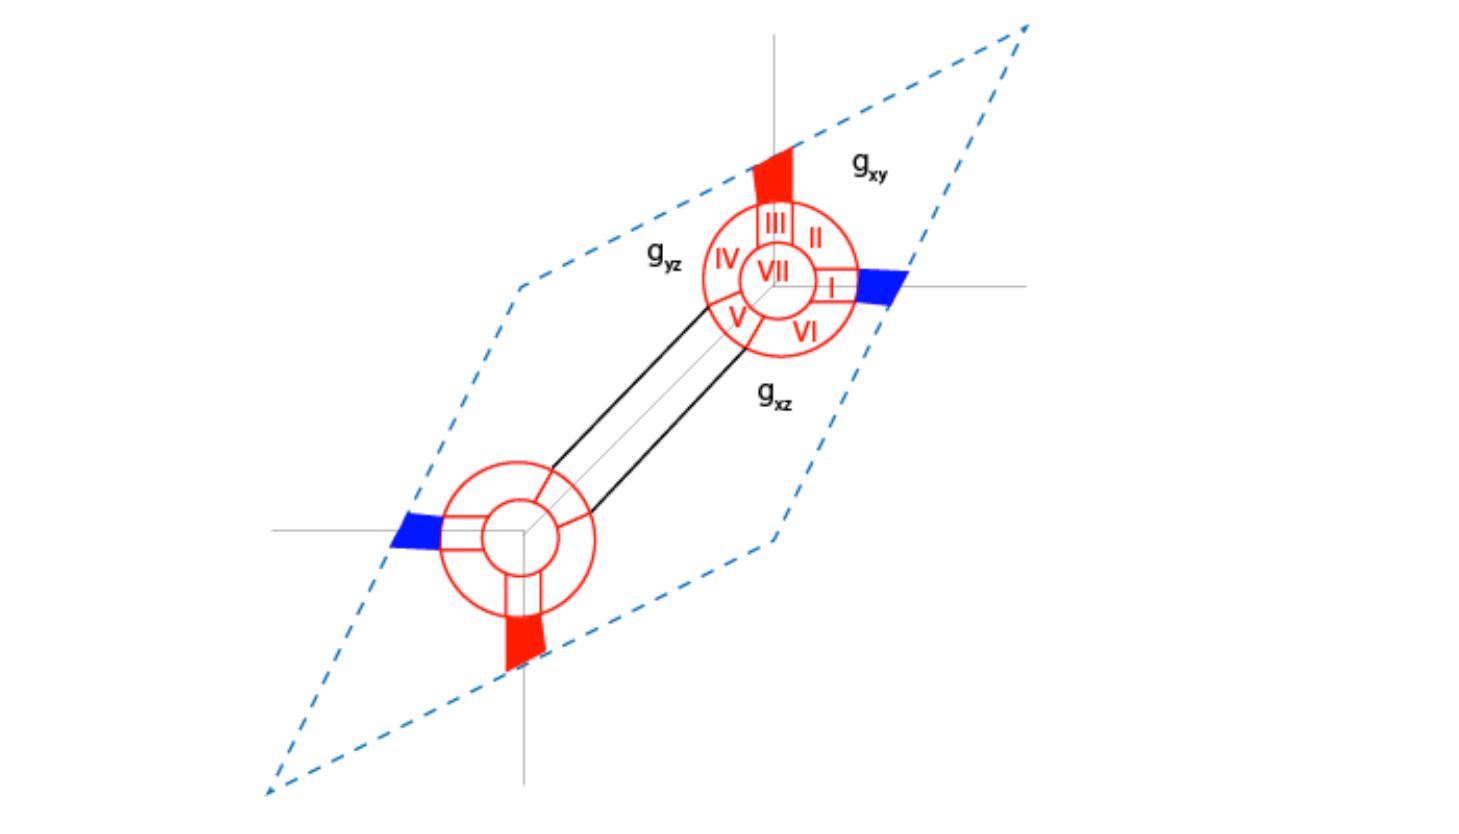
\includegraphics[width=0.62\textwidth]{figures/fig_2_3.png}
\end{figure}

\transnote{此图在原书中没有图号与图注，故这里也不加 \texttt{\textbackslash caption}，以免与原文只有图 2.1、图 2.2 的编号体系冲突。图中虚线框是无界多面体，两个红色小圆是顶点附近的小坐标卡，红色与蓝色箭头分别标出该处起作用的 $g$ 分量。}

还须检验 $|z|$ 很大时得到正定的东西。注意坐标上的等价关系 $\sim$ 正是把坐标看成环簇卡时得到的过渡映射。以 $\PP^2$ 为例：$\C\times\C^*$ 作为各卡的重叠部分落在所有卡内；它在一个卡中的嵌入是 $(u,v)$，在另一个卡中是 $(v^{-1},uv^{-1})$，这就告诉我们过渡映射把 $(u,v)$ 送到另一个。在我们的情形里，先不处理齐次坐标，图景直接给出环簇坐标上的过渡映射。

% ===== 原书 p.69 =====
具体地说，我们希望当 $|v_0|\neq0$ 时找出 $z$ 坐标的中点。固定一个纤维时，这对应于 $(\C^*)^2$ 到自身的环簇卡拼接。那个 $z$ 坐标映到 $T^{-2}z^{-1}$，起点为 $T^{l/3}$。所以我们仍然是把两份 $\C^*$ 互相粘起来，只不过其中一份从半径为 $T^{l/3}$ 的圆开始，而不是只挖掉原点。中点仍是 $T^{-1}$，只是我们粘的是比 $\PP^1$ 情形多挖了一些的平面。于是 $|z|$ 从 $T^{l/3}$ 变到 $T^{-1}$。由于上一项刚检验过的拼接性质，只须检验一半。

\transnote{「只须检验一半」用的正是 $z\mapsto T^{-2}z^{-1}$ 的拼接线对称性：两半的估计互为镜像，若一半上形式正定，另一半随之成立；漏掉这一句会把计算量算成两倍。}

据此检验鼓包函数导数有界。凯勒势形如 $(f+d)+\alpha_4(\theta)\cdot\theta$，所以只须检验 $\alpha_4(\theta)\cdot\theta$ 的导数。这一项可以用上面的计算，理由如下：虽然 $|z|\le T^{-1}$，但可设 $|x|$ 与 $|y|$ 很小。于是 $|T^2xz|\le|Tx|$、$|T^2yz|\le|Ty|$，这些量都很小，它们的对数又有小尺度近似：
\begin{align*}
\theta&=\phi_x-\phi_y\\
&=\log_T(1+|Tx|^2)-\log_T(1+|T^2yz|^2)-\log_T(1+|Ty|^2)+\log_T(1+|T^2xz|^2)\\
&\approx2|Tx|^2-2|Ty|^2\\
\frac{1}{r_*}\frac{\partial}{\partial r_*}(\alpha_4\theta)&=(\alpha_4'\theta+\alpha_4)\frac{\theta_*}{r_*}\\
\frac{\partial}{\partial r_\bullet}(\alpha_4'\theta\theta_*)
&=\alpha_4''\theta_\bullet\theta\theta_*+\alpha_4'\theta_\bullet\theta_*+\alpha_4'\theta\theta_{*\bullet}\\
&=\big(\alpha_4''\theta^2+\alpha_4'\theta\big)\cdot\frac{\theta_\bullet\theta_*}{\theta}
+{\alpha_4'}^{\log}\theta_{*\bullet}\\
\frac{\partial}{\partial r_\bullet}(\alpha_4\theta_*)
&=\alpha_4'\theta_\bullet\theta_*+\alpha_4\theta_{*\bullet}\\
&={\alpha_4'}^{\log}\frac{\theta_\bullet\theta_*}{\theta}+\alpha_4\theta_{*\bullet}
\end{align*}
于是需要估计下面三项，然后检查对数导数有足够空间：
\begin{itemize}[leftmargin=2.2em,itemsep=0.25em]
\item $\frac{\theta_*}{r_*}$：
\[
\frac{\theta_x}{r_x}\approx4T^2,\qquad \frac{\theta_y}{r_y}\approx-4T^2,\qquad \frac{\theta_z}{r_z}\approx0.
\]
\item $\frac{\theta_\bullet\theta_*}{\theta}$ 意味着要考虑 $\frac{r_\bullet r_*}{r_x^2-r_y^2}$，因此需要尺寸约束，使 $\alpha_4$ 的支撑集避开 $r_x=r_y$ 的区域。回想上面已挖掉窄条 $T<(r_x/r_y)^2<1/T$。又因 $\theta$ 近似为 $2T^2(r_x^2-r_y^2)$，只要 $*$ 与 $\bullet$ 都不是 $z$，这一项就近似为零。与前面一样，按两个变量中较大者分别除以 $r_x^2$ 或 $r_y^2$，于是分子至多为 $1$，分母由约束 $T<(r_x/r_y)^2<1/T$ 有正下界。
\item 除 $*=\bullet$ 外，$\theta_{*\bullet}$ 近似为零；而 $*=\bullet$ 时它是常数，故有界。
\end{itemize}
注意对数导数会有足够空间，因为 $r_x$、$r_y$ 很小时 $\theta\approx2T^2(r_x^2-r_y^2)$；这一点在早先按 $\theta\approx T^2(r_x^2-r_y^2)$ 检验时已经做过。

% EN48 c05 | 原书 p.70–81（PDF 79–90） | 第 3 章（无小节）
% 边界：本章自原书 p.70 章首起，至 p.81 最后一条结果收尾；第 4 章自 p.82 起。
\section{阿贝尔簇 $V$ 与 $\Vdual$ 的同调镜像对称}

% ===== 原书 p.70 =====
环面的 SYZ 镜像属于族 Floer 理论（Family Floer theory）的一个例子 [Fuk02]。特别地，
族 Floer 理论表明，线丛应当镜像拉格朗日（子流形）的行为。原因在于：由 Serre 对偶有
$\mathrm{Ext}^1(\OO_{p_0},\OO)\iso\OO_{p_0}$，而环面上竖直的线性拉格朗日（子流形）
与任意其他有限斜率的线性拉格朗日（子流形）恰交于一点。我们可以对每个点定义一个
线丛，使之对应 Floer 理论一侧由该交点生成的一维向量空间；再在所得对象上赋予全纯
结构，即得全纯线丛，参看 [Fuk02]。由于 $\LL_{pt}$ 与有限斜率的线性拉格朗日（子流形）
恰有一个交点，我们可以由此构造一个秩 $1$ 的线丛。

\transnote{$\mathrm{Ext}^1(\OO_{p_0},\OO)\iso\OO_{p_0}$ 是 Serre 对偶的具体形态：
阿贝尔曲面上「点层」的一阶扩张仍是一维的。正因每个交点只贡献一维，交点个数才恰好
等于线丛一侧的态射维数。这也是下文把「交点生成的向量空间」当作纤维的动机。}

\medskip\noindent\textbf{深谷范畴 $\mathrm{Fuk}(\Vdual)$}\par

我们考虑深谷范畴 $\mathrm{Fuk}(\Vdual)$（一个 $A_\infty$-范畴）的如下全子范畴。

\begin{itemize}[leftmargin=2.2em,itemsep=0.25em]
\item 对象：令 $M=\begin{pmatrix}2&1\\1&2\end{pmatrix}$，$\Gamma_B:=M(\Z^2)$。在
  $v_0\colon Y\to\C$ 的纤维 $\Vdual$ 上有仿射作用--角坐标（affine action-angle
  coordinates）$(\xi_1,\xi_2,\theta_1,\theta_2)$，其中 $\xi_i$ 关于复坐标的范数单调，
  $\theta_i$ 是相应的辐角。在这些坐标下，纤维上的辛形式为 $\omega=\de\xi\wedge\de\theta$。
  我们考虑以如下线性拉格朗日（子流形）为对象的子范畴：
\[
\ell_i=\bigl\{(\xi_1,\xi_2,-i\cdot M^{-1}(\xi))\bigr\}_{\xi\in T_B=\R^2/M(\Z^2)}.
\]
  这些对象是 [PZ98] 中椭圆曲线上斜率 $i$ 的直线的类比。
\item 态射：设 $|i-j|\ge1$，则
  $\Hom(\ell_i,\ell_j):=\bigoplus_{p\in\ell_i\cap\ell_j}\C\cdot\{p\}\iso\C^{(i-j)^2}$，
  论证是模算术（modular arithmetic）的。注意这等于 $j>i$ 时的
  $h^0(V,\LL^{\otimes(j-i)})$，而 $i>j$ 时为 $h^2(V,\LL^{\otimes(j-i)})$；
  后一事实将告诉我们各态射群同构。若 $\xi$ 是 $\ell_i$ 上的坐标、$\tilde\xi$ 是
  $\ell_j$ 上的坐标，则交点只能出现在满足下式处：

% ===== 原书 p.71 =====
\begin{equation}\label{eq:3-1}
\begin{gathered}
1)\ \xi\equiv\tilde\xi\mod M(\Z^2)\\
2)\ i\cdot M^{-1}(\xi)\equiv j\cdot M^{-1}(\tilde\xi)\mod\Z^2\\
\Longrightarrow\ i\cdot\xi\equiv j\cdot\tilde\xi\equiv j\cdot\xi\mod M(\Z^2)\\
\Longrightarrow\ \xi\in\frac{1}{i-j}M(\Z^2)
\end{gathered}
\end{equation}
  于是令 $\xi=s(2,1)+t(1,2)$。此时 $(i-j)s$ 与 $(i-j)t$ 可取 $0$ 到 $i-j-1$ 之间的
  任意值，于是得到 $(i-j)^2$ 个交点。
\item $\hom$ 上的 $\mu^1$：微分计数交点之间的全纯双边形（bigon）。
\end{itemize}

\transnote{式~\eqref{eq:3-1} 的推导只用到一个事实：$M$ 是整矩阵。由 1) 知
$j\xi\equiv j\tilde\xi\pmod{M(\Z^2)}$；由 2) 乘以 $M$ 得
$i\xi\equiv j\tilde\xi\pmod{M(\Z^2)}$。两式相减得 $(i-j)\xi\in M(\Z^2)$，即
$\xi\in\frac{1}{i-j}M(\Z^2)$。该有限子群在 $T_B$ 中恰有 $(i-j)^2$ 个元素，
这正是交点数。}

\begin{claim}\label{claim:no-bigons}
对 $i\ne j$，$T^4$ 上线性拉格朗日子流形 $\ell_i\cap\ell_j$ 的任意两个交点之间都
没有双边形，因此 $\mu^1=0$。
\end{claim}

\begin{proof}
由偶对 $(T^4,\ell_i\cup\ell_j)$ 有
\[
0=\pi_2(T^4)(=\pi_2(\R^4))\to\pi_2(T^4,\ell_i\cup\ell_j)\to\pi_1(\ell_i\cup\ell_j)
\xrightarrow{\ \sim\ }\pi_1(T^4),
\]
故 $\pi_2(T^4,\ell_i\cup\ell_j)$ 平凡。于是任何这样的全纯盘都是可缩的。取 $T^4$ 上
以 $\ell_i\cup\ell_j$ 为边界、连接交点 $p,q$ 的双边形
$u\colon D^2\setminus\{\pm1\}\to T^4$。取提升 $\tilde\ell_i,\tilde\ell_j$，使提升后的
交点 $\tilde p=0$：
\[
\tilde\ell_i=\bigl\{(\xi_1,\xi_2,i\cdot M^{-1}(\xi))\bigr\}_{\xi\in\R^2}.
\]
设 $\partial_1,\partial_2$ 是 $D^2\setminus\{\pm1\}$ 的两个边界分支，分别映到
$\ell_i,\ell_j$。把 $u(\partial_i)$ 提升到 $\R^4$，记作 $\gamma_1,\gamma_2$，使
$\gamma_i(0)=\tilde p$，并令 $\tilde q_i:=\gamma_i(1)$。由盘的可缩性，
$\tilde q_1=\tilde q_2$。然而
\[
\tilde\ell_i\cap\tilde\ell_j
\Longrightarrow \xi^{(i)}=\xi^{(j)}=:\xi,\qquad i\xi=j\xi\ \therefore\ \xi=0,
\]
因为 $|i-j|\ge2$。所以至多只有一个交点，而非非平凡双边形所需的两点。
\end{proof}

% [Tutor Note: 断言只假设 i ≠ j，此处证明却用 |i−j| ≥ 2；当 |i−j| = 1 时由
% (i−j)ξ = 0 同样得 ξ = 0，结论不受影响。原书如此，保留。]

\transnote{证明的关键是「可缩」二字：盘可缩，故两个边界分支的端点提升后必须重合。
若存在非平凡双边形，两个端点应给出两个不同的交点，与唯一性矛盾。注意此处
$\tilde\ell_i$ 与 $\tilde\ell_j$ 是 $\R^4$ 中的平面，等式 $i\xi=j\xi$ 中的乘法是
数乘而非模运算，这正是可取 $\xi=0$ 的原因。}

% ===== 原书 p.72 =====
对相异的 $i,j$，态射空间维数为 $(i-j)^2$；仅当 $j>i$ 时它与
$h^0(V,\LL^{j-i})$ 相符，否则这些态射处于 Floer 次数 $2$，与
$h^2(V,\LL^{j-i})$（负线丛）相符。

另一方面，$i=j$ 时，$\ell_i$ 与它的小哈密顿扰动之间通常确实存在双边形。尽管如此，
$HF(\ell_i,\ell_i)=H^*(T^2)$ 仍然成立；所依赖的关键几何事实是 $\ell_i$ 在环面内
不围出任何盘，故自 $HF$ 约化为经典上同调。

若 $i=j$，由 PSS 同构（PSS isomorphism）有
$CF^*(\ell_i,\ell_i)=HF^*(\ell_i,\ell_i)$。于是
$HF^*(\ell_i,\ell_i)\iso H^*(\ell_i)=H^*(T^2)$。因此所有情形下都有
$HF^*(\ell_i,\ell_j)\iso\mathrm{Ext}^*_V(\LL^{\otimes i},\LL^{\otimes j})$。

\transnote{「不围出盘」为何足以让自 $HF$ 退化为经典上同调：没有盘，就不存在连通
两个交点的伪全纯盘，微分 $\mu^1$ 消失；再取哈密顿量为 Morse 函数并作小扰动，
Floer 复形便与奇异上同调同构。这也解释了 $i=j$ 时虽然有双边形、但 $\mu^1$ 仍可
取零的微妙之处：那些双边形在扰动极限下成对抵消。}

\begin{itemize}[leftmargin=2.2em,itemsep=0.25em]
\item 复合，即 $\hom$ 上的 $\mu^2$（与 [PZ98] 中椭圆曲线的图景类比）：我们考虑
  提升 $\tilde\ell_0,\tilde\ell_1,\tilde\ell_2$，考察可能出现的三角形。所得结果是
  一个以 $\Gamma$ 中元素为下标的和式，与多 $\theta$ 函数（multi-theta functions）
  的展开相符。
\item 单位态射：$\hom(\ell_i,\ell_i)\iso H^*(V,\ell_i)$，它自然带有单位元，但我
  认为这还需要更多工作。通常的做法是证明它同构于 Morse 复形（Morse complex）：
  取哈密顿量为 Morse 函数，然后考察 $\de f$。临界点对应 $\de f=0$ 处，在 Floer
  框架中给出交点；Morse 轨道也是常 $t$ 的 Floer 轨道，在这个特殊情形下 Floer
  方程与 Morse 方程恰好一致。哈密顿扰动在纤维内有效，尽管后文会看到它在全空间内
  无效。
\end{itemize}

% [Tutor Note: 原文写作 hom(ℓi, ℓi) ≅ H*(V, ℓi)，把拉格朗日 ℓi 当作「V 上的层」
% 来写上同调，记号略欠严格；按上下文应为 H*(ℓi)。保留原样。]

\medskip\noindent\textbf{有界导出范畴 $\DBCoh(V)$}\par

\begin{definition}\label{def:bounded-derived}
有界导出范畴（bounded derived category）的定义如下。令 $\cA$ 为 $V$ 上相干层
构成的范畴。注意 $V$ 是阿贝尔簇，从而是射影簇。
\end{definition}

\begin{claim}\label{claim:A-abelian}
$\cA$ 是阿贝尔范畴，特别地有核与余核，因此可以定义对象的链复形。
\end{claim}

\begin{definition}\label{def:kom}
令 $\mathrm{Kom}(\cA)$ 为 $\mathrm{Coh}(V)$ 中链复形构成的范畴，态射为链映射，
复合为链映射的复合。
\end{definition}

% [Tutor Note: 上一段应写「A 中链复形」；原文误写 Coh(V)，且此处 A 与 Coh(V) 本应
% 是同一范畴。保留原样。]

\begin{definition}\label{def:k-category}
令 $K(\cA)$ 的对象为如上链复形，态射则在同伦等价这一等价关系 $\sim$ 下等同。
\end{definition}

\begin{definition}\label{def:derived}
导出范畴 $D(\cA)$ 与 $K(\cA)$ 有相同的对象；态射 $A^\bullet\to B^\bullet$ 是一个
roof $A^\bullet\leftarrow C^\bullet\to B^\bullet$，其中 $C^\bullet\to A^\bullet$
是拟同构（quasi-isomorphism），即在上同调上诱导同构的链映射。若两个态射在
$K(\cA)$ 中同为第三个体所支配，则它们等价。
\end{definition}

% [Tutor Note: 「被第三个体所支配」原文作 dominated in K(A) by a third object of the
% same sort，这是导出范畴局部化的标准构造，但原文未给出「支配」的精确定义。保留原样，
% 读者可按 [Wei94, §10.4] 的 roof 等价关系理解。]

于是以 $\mathrm{Kom}^{\mathrm{b}}(\cA)$ 为起点执行上述过程，即只取有界链复形
（在有限多个对象之外为零），便得到有界导出范畴。

\begin{claim}\label{claim:dg-enhance}
$\DBCoh(V)$ 可以提升为 dg-范畴（dg-category），即满足 $\mu^{\ge3}=0$ 的
$A_\infty$-范畴。
\end{claim}

\transnote{「提升为 dg-范畴」指：除了上同调层面的态射群，还给每个态射空间配上
链复形结构以及满足结合律的复合，使同伦范畴恰好是导出范畴。$\mu^{\ge3}=0$ 表示
只有 $\mu^1$（微分）与 $\mu^2$（复合），故不必处理高阶运算，这正是导出范畴
「是 dg-范畴」的意思。}

% ===== 原书 p.73 =====
此处我们不需要这一点，因为在我们的设定中深谷范畴上 $\mu^1=0$，故可以证明普通
范畴之间的等价。

\begin{claim}\label{claim:split-generate}
回忆此前定义的 $\LL\to V$。我们断言 $\OO,\LL,\LL^2$ 分裂生成（split-generate）
$\DBCoh(V)$。
\end{claim}

\begin{remark}\label{rem:higher-products}
这使我们只需考虑这些对象，但代价是需要关于更高 $A_\infty$ 积的更多信息。原因是
其他对象将作为由 $\OO,\LL,\LL^2$ 构造的复形出现，而计算这些复形之间上同调层面的
$\hom$ 需要知道 $\OO,\LL,\LL^2$ 之间某些链层面的更高复合。特别地，原则上需要知道
所有涉及从 $\OO,\LL,\LL^2$ 中任取的对象序列的 $\mu^k$，且这些对象可任意重复。
\end{remark}

\begin{claim}\label{claim:ample}
如上定义的 $\LL$ 是丰富线丛（ample line bundle）。
\end{claim}

\begin{proof}
复环面上的线丛由 Hermite 形式 $H$ 刻画（见 Polishchuk 关于阿贝尔簇的书 [Pol03]）。
丰富线丛等价于存在某个 $i$ 使 $H^0(V,\LL^i)\ne0$；本设定正是如此，因为 $i>0$ 时
$\LL^i$ 有 $i^2$ 个截面。此外，映射 $V\ni x\mapsto t_x^*\LL\otimes\LL$ 的核有限，
这等价于 $H$ 非退化（见 [Pol03, 第 8.5--8.6 章]）。但此处
\[
H=\begin{pmatrix}2&1\\1&2\end{pmatrix}
\]
行列式非零，即非退化，故 $\LL$ 丰富，断言成立。
\end{proof}

\begin{corollary}\label{cor:projective}
阿贝尔簇 $V$ 是射影的。
\end{corollary}

为给出分裂生成的定义，先作一些准备。

\begin{definition}\label{def:triangulated}
若范畴 $\cC$ 包含所有映射锥（mapping cone），即对任意态射 $f$，对象
$\mathrm{Cone}(f)$ 是 $\cC$ 中的对象，则称 $\cC$ 是三角的（triangulated）。更
准确地说，它包含平移函子（shift functor），即自等价 $A\mapsto A[1]$，并带有一类
distinguished triangles。
\end{definition}

\begin{definition}\label{def:thick}
三角子范畴 $\cD\subset\cC$ 称为厚的（thick），若它对取直和项封闭，即
$E\oplus F\in\mathrm{Ob}(\cD)\Longrightarrow E,F\in\mathrm{Ob}(\cD)$。
\end{definition}

\begin{definition}\label{def:split-generate}
若一组对象 $\{G_i\}_{i\in I}\in\mathrm{Ob}(\cC)$ 的厚包络（thick envelope）是
$\cC$，即取包含诸 $G_i$ 且对取直和项封闭的最小三角范畴得到整个 $\cC$，则称它们
分裂生成 $\cC$。
\end{definition}

\begin{proof}[断言~\ref{claim:split-generate} 的证明]
以下论证来自 MSRI 导出范畴暑期学校 [APS, 第 5.3 讲]。每个复形由其上的上同调生成，
故只需证明任意相干层 $F$ 落在 $\OO,\LL,\LL^2$ 的厚包络中；这样 $\DBCoh(V)$ 的
每个元素都会被厚包络达到，换言之 $\OO,\LL,\LL^2$ 分裂生成。

% ===== 原书 p.74 =====
我们已看到 $V$ 是射影的，因而 $\mathrm{Coh}(V)$ 有足够多的局部自由层（文献）。
特别地，$n$ 充分大时 $F(n)$ 由整体截面生成，即有满射
$\OO_X^n\twoheadrightarrow F(n)$；于是扭以 $\OO(-n)$、并对
$\OO_X(-n)^n\to F$ 的核重复此过程，便得到 $F$ 的局部自由消解：
\[
\cdots\to P^{-N}\to P^{-N+1}\to\cdots\to P^0\to F\to0.
\]
令 $Q$ 为截断至次数 $N$ 所得的复形：
\[
Q:=[P^{-N}\to\cdots\to P^{-1}\to P^0].
\]
则 $Q$ 落在厚包络 $\langle\OO,\LL,\LL^2\rangle$ 中，因为所有 $P^i$ 都以 $\LL^i$
为直和项，而 $\langle\OO,\LL,\LL^2\rangle$ 是完全例外收集体（full exceptional
collection）（文献），包含 $\LL$ 的所有幂。有复形的包含 $P^\bullet\to Q$，其商为
\[
G[N+1]=\cdots\to P^{-N-1}\to0\to0\cdots\to0,
\]
其中 $G$ 定义为次数 $-N-1$ 的上同调，因为复形其余部分正合。特别地，$G$ 是相干层，
且得到态射
\[
F\to G[N+1]\in\mathrm{Ext}^{N+1}(F,G)\iso
\mathrm{Ext}^{2-N-1}(G,F\otimes\omega)^*=0,
\]
最后一步用 Serre 对偶。于是有
\[
G[N]\longrightarrow Q\longrightarrow F\xrightarrow{\ 0\ }G[N+1],
\]
由此 $Q\iso G[N]\oplus F$。已知 $Q$ 在厚包络中，而厚包络对直和项封闭，故 $F$ 也
在其中，证毕。
\end{proof}

\transnote{此证明是本章的技术核心，可拆成三步读。其一，用射影性得到局部自由消解，
把 $F$ 换成有限复形 $Q$；其二，用 Serre 对偶把 $\mathrm{Ext}^{N+1}(F,G)$ 消成零，
从而让短正合列分裂，得到 $Q\cong G[N]\oplus F$；其三，厚包络对直和项封闭，于是
$F$ 作为 $Q$ 的直和项也在其中。三步缺一不可。}

因此，只需在 $\OO,\LL,\LL^2$ 上考察函子，即可证明范畴的全忠实嵌入，代价是需要
知道更高的 $A_\infty$ 积。

\medskip\noindent\textbf{走向 HMS：全忠实嵌入
$\DBCoh(V)\hookrightarrow\mathrm{Fuk}(\Vdual)$}\par

函子 $\DBCoh(V)\to\mathrm{Fuk}(\Vdual)$ 如下。在对象上，
$\LL^{\otimes k}\mapsto\ell_k$。回忆 §1.2 的基公式（原书 1.2.17）：$H^0(V,\LL^{\otimes l})$ 有以下
截面基：
\[
s_{e,l}:=\sum_\gamma\tau^{-l\kappa(\gamma+\frac{\gamma_{e,l}}{l})}
x^{-l\lambda(\gamma)-\gamma_{e,l}}.
\]

% [Tutor Note: 原书此式末项印作 −γ_{e,l}，漏写 λ；按原书 1.2.17 以及本页下方乘积
% 公式，正确形式应为 x^{−λ(lγ+γ_{e,l})}，即指数末项为 −λ(γ_{e,l})。此处照原书排印，
% 不作改动。]

\transnote{上式指数末项在原书三处排印不一：p.74 印作
$-\gamma_{e,l}$，p.77 的同一基印作 $x^{-\lambda(l\gamma-\gamma_{e,l})}$，而原书
1.2.17 印作 $x^{-l\lambda(\gamma)-\lambda(\gamma_{e,l})}$。三者中只有最后一式
（等价于 $x^{-\lambda(l\gamma+\gamma_{e,l})}$）与下面的乘积公式自洽。阅读时以
原书 1.2.17 为准。}

% ===== 原书 p.75 =====
其中 $\gamma_{e,l}=s\gamma'+t\gamma''$，$0\le s,t<l$。于是在态射上，函子的作用
如下（$s_i$ 记 $\gamma_{e,l}$ 的各种取法）：
\begin{align*}
\hom(\OO,\LL)=H^0(V,\LL)\ni s&\mapsto
p\in\hom(\ell_0,\ell_1)=\bigoplus_{p\in\ell_0\cap\ell_1}\C\cdot p=\C\cdot p,\\
\hom(\OO,\LL^2)=H^0(V,\LL^2)\ni(s_1,s_2,s_3,s_4)&\mapsto
(p_1,p_2,p_3,p_4)\in\bigoplus_{p\in\ell_0\cap\ell_2}\C\cdot p,\\
&\qquad\text{此处 }|\ell_0\cap\ell_2|=4,\\
\hom(\LL,\LL^2)\iso\hom(\OO,\LL^*\otimes\LL^2)&\iso\hom(\OO,\LL)
=H^0(V,\LL)\\
&\qquad\ni s\mapsto p'\in\hom(\ell_1,\ell_2)=\C\cdot p'.
\end{align*}
与复合相容，即：
\begin{gather*}
s(x)=\sum_\gamma\tau^{-\kappa(\gamma)}x^{-\lambda(\gamma)},\qquad
s^2(x)=\sum_{\tilde\gamma,\tilde{\tilde\gamma}}
\tau^{-\kappa(\tilde\gamma)-\kappa(\tilde{\tilde\gamma})}
x^{-\lambda(\tilde\gamma)-\lambda(\tilde{\tilde\gamma})},\\
\hom(\LL,\LL^2)\otimes\hom(\OO,\LL)\ni s^2(x)=c_1s_1+c_2s_2+c_3s_3+c_4s_4\\
\longleftrightarrow\ \mu^2(p,p')=c_1p_1+c_2p_2+c_3p_3+c_4p_4.
\end{gather*}
特别地，我们预期系数 $c_i$ 是某个特定 $x$ 值的 $\theta$ 函数 $s(x)$，类比
[PZ98] 的计算。我们希望用 $H^0(V,\LL^2)$ 的这组基表示 $s^2(x)$。把 $s^2(x)$ 的
和式按 $\tilde\gamma+\tilde{\tilde\gamma}$ 中 $(\gamma',\gamma'')$ 系数对的四种
可能奇偶性拆成四个和。然后作坐标变换
\[
\gamma=\tfrac12(\tilde\gamma+\tilde{\tilde\gamma}-\gamma_e),\qquad
\eta=\tfrac12(\tilde{\tilde\gamma}-\tilde\gamma-\gamma_e),\qquad
\gamma_e\in\{0,\gamma',\gamma'',\gamma'+\gamma''\}.
\]
例如，若 $\tilde\gamma+\tilde{\tilde\gamma}=(n_1+m_1)\gamma'+(n_2+m_2)\gamma''$
且 $n_1+m_1$、$n_2+m_2$ 均为偶数，则可将 $\tilde\gamma+\tilde{\tilde\gamma}$ 写成
某个 $\gamma\in\Gamma_B$ 的 $2\gamma$。若二者一奇一偶，则须减去 $\gamma'$，等等。
这样得到 $\gamma_e$ 的四种取法。于是可按四种奇偶选择把 $s^2(x)$ 拆成四个和，
用诸 $s_i(x)$ 表示。

% ===== 原书 p.76 =====
再回忆二次型 $\kappa$ 满足
$\kappa(\gamma+\eta)=\kappa(\gamma)+\kappa(\eta)-\ip{\gamma}{\lambda(\eta)}$。
\begin{align*}
s^2(x)&=\sum_{\tilde\gamma,\tilde{\tilde\gamma}}
\tau^{-\kappa(\tilde\gamma)-\kappa(\tilde{\tilde\gamma})}
x^{-\lambda(\tilde\gamma+\tilde{\tilde\gamma})}\\
&=\sum_{\gamma,\eta}\Bigl[
\tau^{-\kappa(\gamma-\eta)-\kappa(\gamma+\eta)}x^{-2\lambda(\gamma)}\\
&\qquad+\tau^{-\kappa(\gamma+\gamma'/2-\eta-\gamma'/2)
-\kappa(\gamma+\gamma'/2+\eta+\gamma'/2)}x^{-2\lambda(\gamma)}x_1^{-1}\\
&\qquad+\tau^{-\kappa(\gamma+\gamma''/2-\eta-\gamma''/2)
-\kappa(\gamma+\gamma''/2+\eta+\gamma''/2)}x^{-2\lambda(\gamma)}x_2^{-1}\\
&\qquad+\tau^{-\kappa(\gamma+(\gamma'+\gamma'')/2-\eta-(\gamma'+\gamma'')/2)
-\kappa(\gamma+(\gamma'+\gamma'')/2+\eta+(\gamma'+\gamma'')/2)}
x^{-2\lambda(\gamma)}(x_1x_2)^{-1}\Bigr]\\
&=\sum_\eta\tau^{-2\kappa(\eta)}\sum_\gamma\tau^{-2\kappa(\gamma)}x^{-2\lambda(\gamma)}\\
&\qquad+\sum_\eta\tau^{-2\kappa(\eta+\gamma'/2)}\sum_\gamma
\tau^{-2\kappa(\gamma+\gamma'/2)}x^{-2\lambda(\gamma)}x_1^{-1}\\
&\qquad+\sum_\eta\tau^{-2\kappa(\eta+\gamma''/2)}\sum_\gamma
\tau^{-2\kappa(\gamma+\gamma''/2)}x^{-2\lambda(\gamma)}x_2^{-1}\\
&\qquad+\sum_\eta\tau^{-2\kappa(\eta+(\gamma'+\gamma'')/2)}
\sum_\gamma\tau^{-\kappa(\gamma+(\gamma'+\gamma'')/2)}x^{-2\lambda(\gamma)}
(x_1x_2)^{-1}\\
&=\sum_\eta\tau^{-2\kappa(\eta)}s_1
+\sum_\eta\tau^{-2\kappa(\eta+\gamma'/2)}s_2\\
&\qquad+\sum_\eta\tau^{-2\kappa(\eta+\gamma''/2)}s_3
+\sum_\eta\tau^{-2\kappa(\eta+(\gamma'+\gamma'')/2)}s_4.
\end{align*}

\transnote{这一段只做了一件事：把 $s^2(x)$ 按 $\gamma_e\in\{0,\gamma',\gamma'',
\gamma'+\gamma''\}$ 分成四组，再用 $\kappa$ 的极化恒等式把每组的指数化成
「只含 $\eta$ 的因子 × 只含 $\gamma$ 的因子」。四组的 $\eta$ 因子恰是四个
$\tau$ 级数，$\gamma$ 因子恰是四个加权的 $s_i$，于是 $s^2(x)=\sum_i C_i s_i$。
四个系数 $C_i$ 正是后面要数三角形的对象。}

\begin{claim}\label{claim:coeff-triangle}
诸 $s_i$ 上的系数与三角形计数相符，即与深谷范畴中的 $\mu^2$ 相符。
\end{claim}

\begin{proof}
用 $\tilde{\ }$ 记到万有覆盖 $\R^4$ 的提升。把 $\tilde\ell_0\cap\tilde\ell_2$
放在三角形中的位置有四种选择（其他选择在阿贝尔簇上给出相同的三角形）。由
式~\eqref{eq:3-1} 的计算，取
\[
\tilde p_e=(\gamma_e/2,2M^{-1}(\gamma_e/2))=(\gamma_e/2,\lambda(\gamma_e)),
\]
因为 $\lambda$ 是线性映射 $M^{-1}$。已知 $p=\ell_0\cap\ell_1$ 的提升 $\tilde p$
必落在过 $\tilde p_e$ 的 $\tilde\ell_0$ 上。沿 $\tilde\ell_0$ 后两个坐标不变，
故 $\lambda(\gamma_e)$ 就是角坐标；又 $\tilde p$ 位于 $(0,0)$ 之上，故第一个坐标
是某个 $\eta\in\Gamma_B$：
\[
\tilde p=(\eta,\lambda(\gamma_e)).
\]
若 $\tilde p$ 位于 $(0,0)$，则 $p'=\ell_1\cap\ell_2$ 的提升是某个
$(\xi,M^{-1}(\xi))=(\xi,\lambda(\xi))$，因为 $\tilde\ell_2$ 会过原点（设拉格朗日
按顺时针排列）。由于它可能被 $(\eta,\lambda(\gamma_e))$ 平移，得到
$\tilde p'=(\eta,\lambda(\gamma_e))+(\xi,\lambda(\xi))$，其中 $\xi$ 由
$\overrightarrow{\tilde p'\tilde p_e}$ 落在 $\tilde\ell_2$ 上确定，即角度改变
$2\lambda$：
\[
\overrightarrow{\tilde p'\tilde p_e}
=\ip{\eta+\xi-\gamma_e/2}{\lambda(\gamma_e+\xi)-\lambda(\gamma_e)}
\]
\[
\Longrightarrow\ 2\lambda(\eta+\xi-\gamma_e/2)=\lambda(\xi)
\ \therefore\ \xi=\gamma_e-2\eta,\qquad
\therefore\ \tilde p'=(\gamma_e-\eta,2\lambda(\gamma_e-\eta)).
\]
\end{proof}

% ===== 原书 p.77 =====
\begin{figure}[htbp]
\centering
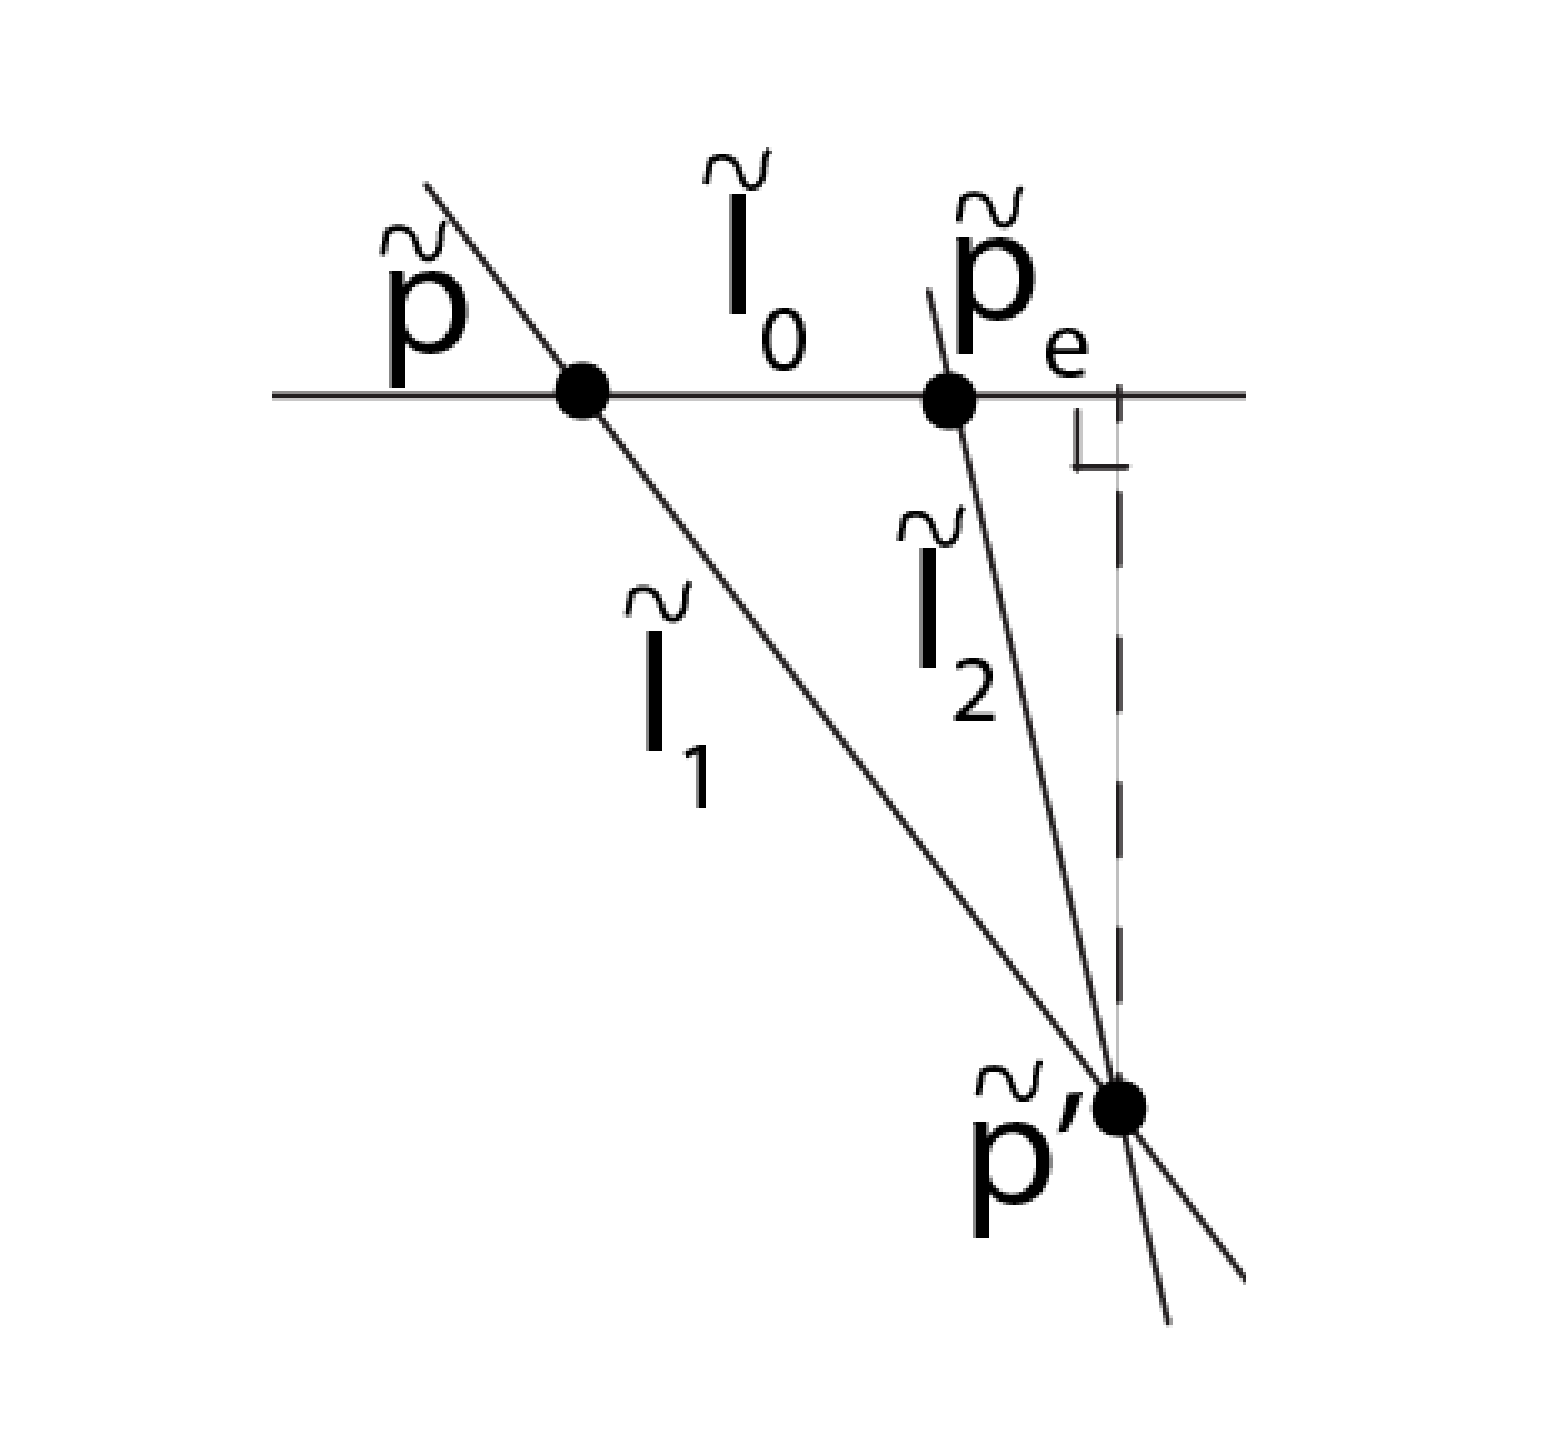
\includegraphics[width=0.42\textwidth]{figures/fig_3_1.png}
\caption{椭圆曲线情形中的三角形，以及 $T^4$ 情形的代表（原书 p.77）}
\label{fig:3-1}
\end{figure}

现在三角形已有三个点，我们要求它的面积。受椭圆曲线情形的图景启发（见图~\ref{fig:3-1}），
若把 $\tilde p_e$ 沿 $\tilde p_e$ 与 $\tilde p$ 的连线向远离 $\tilde p$ 的方向
延长同样的距离，便得到直角三角形。这可由三边构成勾股三元组看出：
\[
|\eta-\gamma_e/2|^2+|\lambda(\gamma_e-2\eta)|^2=(\text{第三边长})^2.
\]
于是取底边的一半与同样的高，得到三角形面积
\[
\frac12\int_\Delta\de\xi\wedge\de\theta
=\ip{(\eta-\gamma_e/2)}{\lambda(\eta-\gamma_e/2)}
=-2\kappa(\eta-\gamma_e/2).
\]
这与复侧 $\tau$ 的指数一致，断言证毕。

\transnote{面积公式把辛几何与复几何接了起来：左边是三角形在 $(\xi,\theta)$ 平面中
的辛面积，右边是二次型 $\kappa$ 在 $\eta-\gamma_e/2$ 处的取值。请注意 $\kappa$ 是
负定的（在第一 Chern 类的尺度下），故当 $\eta\ne\gamma_e/2$ 时右边为正，与面积
的符号一致；$-\!2\kappa$ 前面的负号正是由此而来。}

下面要证明乘法在更一般的情形 $i<j<k$ 下相符。先考虑线丛。有
$\Hom(\LL^i,\LL^j)\iso H^0(V,\LL^{j-i})$，故令 $l:=j-i$，$l':=k-j$。取
$\LL^l$ 的如下基：
\[
s_{e,l}:=\sum_\gamma\tau^{-l\kappa(\gamma+\frac{\gamma_{e,l}}{l})}
x^{-\lambda(l\gamma-\gamma_{e,l})}.
\]

% [Tutor Note: 与 p.74 的基是同一对象，原书此处印作 x^{−λ(lγ−γ_{e,l})}，括号内
% 符号应为 +（即 x^{−λ(lγ+γ_{e,l})}）。下方乘积公式与此不符时无法推出，故按原书
% 排印并加注；正确形式见原书 1.2.17。]

特别地，$\gamma_{e,l}=s\gamma'+t\gamma''$（$0\le s,t<l$），给出
$H^0(V,\LL^l)$ 的 $l^2$ 个基元素。我们希望用 $H^0(V,\LL^{l+l'})$ 的基表示两个
这样的截面之积，并把系数与另一侧的三角形计数比较。
\[
s_{e,l}\cdot s_{e,l'}=\sum_{\tilde\gamma,\tilde{\tilde\gamma}}
\tau^{-l\kappa(\tilde\gamma+\frac{\gamma_{e,l}}{l})
-l'\kappa(\tilde{\tilde\gamma}+\frac{\gamma_{e,l'}}{l'})}
x^{-\lambda(l\tilde\gamma+\gamma_{e,l}+l'\tilde{\tilde\gamma}+\gamma_{e,l'})}.
\]

% ===== 原书 p.78 =====
我们希望用 $H^0(V,\LL^{l+l'})$ 的类似基表示它：
\[
s_e:=\sum_\gamma\tau^{-(l+l')\kappa(\gamma+\frac{\gamma_e}{l+l'})}
x^{-(l+l')\lambda(\gamma+\frac{\gamma_e}{l+l'})}.
\]
把乘积中 $x$ 的幂与之比较，我们这样定义 $\gamma$：把和
$l\tilde\gamma+\gamma_{e,l}+l'\tilde{\tilde\gamma}+\gamma_{e,l'}$ 看作
$(l+l')\Gamma_B$ 中的元素加一个余项 $\gamma_e$。即令该元素为 $\gamma\in\Gamma_B$，
余项记为 $\gamma_e$：
\[
(l+l')\gamma+\gamma_e:=l\tilde\gamma+\gamma_{e,l}
+l'\tilde{\tilde\gamma}+\gamma_{e,l'}.
\]
类比上面的 $(i,j,k)=(0,1,2)$ 情形，我们希望用新变量 $A,B$ 作坐标变换，使 $\tau$
的指数满足等式
\[
\Bigl(\tilde\gamma+\frac{\gamma_{e,l}}{l},\ 
\tilde{\tilde\gamma}+\frac{\gamma_{e,l'}}{l'}\Bigr)
=\Bigl(A-\frac{B}{l},\ A+\frac{B}{l'}\Bigr),
\]
因为
$-l\kappa(A-\frac{B}{l})-l'\kappa(A+\frac{B}{l'})
=-(l+l')\kappa(A)-(\frac1l+\frac1{l'})\kappa(B)$。我们希望
$A=\gamma+\frac{\gamma_e}{l+l'}$，而它确实成立。$B$ 应当是变量 $\eta$ 与余项的
函数，使得 $\eta\in\Gamma_B$。我们作如下定义；它确实满足要求，其动机在下面的
三角形计数中会变得清楚：
\[
B=\frac{ll'}{l+l'}\Bigl(\tilde\gamma+\frac{\gamma_{e,l}}{l}
-\tilde{\tilde\gamma}-\frac{\gamma_{e,l'}}{l'}\Bigr)
=:\eta-\frac{l\gamma_e}{l+l'}.
\]

\begin{claim}\label{claim:eta-lattice}
$\eta\in\Gamma_B$。
\end{claim}

\begin{proof}
\[
\eta=\frac{ll'}{l+l'}\Bigl(\tilde\gamma+\frac{\gamma_{e,l}}{l}
-\tilde{\tilde\gamma}-\frac{\gamma_{e,l'}}{l'}\Bigr)+\frac{l\gamma_e}{l+l'}
\]
\[
=\frac{1}{l+l'}\bigl(ll'\tilde\gamma+l'\gamma_{e,l}
-ll'\tilde{\tilde\gamma}-l\gamma_{e,l'}-l(l+l')\gamma
+l^2\tilde\gamma+l\gamma_{e,l}+ll'\tilde{\tilde\gamma}+l\gamma_{e,l'}\bigr)
=l\tilde\gamma+\gamma_{e,l}-l\gamma\in\Gamma_B.
\]
\end{proof}

% [Tutor Note: 原书此证明以划掉符号标出相消的两项 ll′γ̃̃ 与 −lγ_{e,l′}，并靠
% l²γ̃ 与 l(l+l′)γ 两项合并。此处按展开式排印，划掉痕迹从略。]

\begin{corollary}\label{cor:product-basis}
\begin{align*}
s_{e,l}\cdot s_{e,l'}&=\sum_{\tilde\gamma,\tilde{\tilde\gamma}}
\tau^{-l\kappa(\tilde\gamma+\frac{\gamma_{e,l}}{l})
-l'\kappa(\tilde{\tilde\gamma}+\frac{\gamma_{e,l'}}{l'})}
x^{-\lambda(l\tilde\gamma+\gamma_{e,l}+l'\tilde{\tilde\gamma}+\gamma_{e,l'})}\\
&=\sum_{\gamma,\eta}\tau^{-l\kappa\bigl(\gamma+\frac{\gamma_e}{l+l'}
-\frac1l(\eta-\frac{l\gamma_e}{l+l'})\bigr)
-l'\kappa\bigl(\gamma+\frac{\gamma_e}{l+l'}+\frac1{l'}
(\eta-\frac{l\gamma_e}{l+l'})\bigr)}
x^{-(l+l')\lambda(\gamma)-\lambda(\gamma_e)}\\
&=\sum_\eta\tau^{-(\frac1l+\frac1{l'})\kappa(\eta-\frac{l\gamma_e}{l+l'})}
\sum_\gamma\tau^{-(l+l')\kappa(\gamma+\frac{\gamma_e}{l+l'})}
x^{-(l+l')\lambda(\gamma)-\lambda(\gamma_e)}.
\end{align*}
\end{corollary}

% ===== 原书 p.79 =====
\begin{claim}\label{claim:functor-composition}
左竖直函子 $\DBCoh(V)\to\mathrm{Fuk}(\Vdual)$ 与复合相容。
\end{claim}

\begin{proof}
我们把两个截面之积的表达式中的系数与三角形计数作比较。分别取 $p_1,p_2,p_3$ 为
$\ell_i\cap\ell_k$、$\ell_i\cap\ell_j$、$\ell_j\cap\ell_k$ 中的点。
$\ell_i\cap\ell_k$ 有 $(l+l')^2$ 种选择如下：
\[
p_1=\Bigl(\frac{\gamma_e}{k-i},-\frac{k}{k-i}\lambda(\gamma_e)\Bigr).
\]
则 $\overrightarrow{p_2p_1}$ 落在 $\tilde\ell_i$ 上，故形如
$(\xi,-i\lambda(\xi))$。又 $p_2$ 落在 $\ell_i$ 的提升上，故也是这种形式（我们用
$\eta/l$，使 $\eta\in\Gamma_B$ 最终与上面多 $\theta$ 函数中所用的 $\eta$ 一致），
至多相差一个格元素的平移，而该平移是 $(0,\lambda(\gamma_e))$：
\[
p_2=\Bigl(\frac\eta l,-i\lambda\Bigl(\frac\eta l\Bigr)-\lambda(\gamma_e)\Bigr),
\]
\[
\overrightarrow{p_2p_1}=\Bigl(\frac{\gamma_e}{k-i}-\frac\eta l,
-\frac{k}{k-i}\lambda(\gamma_e)+i\lambda\Bigl(\frac\eta l\Bigr)+\lambda(\gamma_e)\Bigr)
=(\xi,-i\lambda(\xi)).
\]
于是 $p_3(A,B)$ 有两个条件如下：
\begin{gather*}
\overrightarrow{p_2p_3}=\Bigl(A-\frac\eta l,
B+i\lambda\Bigl(\frac\eta l\Bigr)+\lambda(\gamma_e)\Bigr)\\
\therefore\ B+i\lambda\Bigl(\frac\eta l\Bigr)+\lambda(\gamma_e)
=-j\lambda\Bigl(A-\frac\eta l\Bigr)\\
\overrightarrow{p_1p_3}=\Bigl(A-\frac{\gamma_e}{k-i},
B+\frac{k}{k-i}\lambda(\gamma_e)\Bigr)\\
\therefore\ B+\frac{k}{k-i}\lambda(\gamma_e)
=-k\lambda\Bigl(A-\frac{\gamma_e}{k-i}\Bigr)
\Longrightarrow\ B=-k\lambda(A)\\
\Longrightarrow\ -k\lambda(A)=-j\lambda(A)+(j-i)\lambda\Bigl(\frac\eta l\Bigr)
-\lambda(\gamma_e)\\
\Longrightarrow\ (k-j)A=(i-j)\frac\eta l+\gamma_e\\
\therefore\ A=\frac{i-j}{k-j}\frac\eta l+\frac{1}{k-j}\gamma_e
=-\frac1{l'}\eta+\frac1{l'}\gamma_e,\qquad B=-k\lambda(A).
\end{gather*}
我们令 $\zeta:=-\frac\eta l+\frac{\gamma_e}{l+l'}$，因为这个表达式多处出现。为求
三角形的辛面积（在同伦不变性下相同，即对以这些点为顶点的任意全纯三角形相同），
我们取 $\frac12\int_P\de\xi\wedge\de\theta$，其中 $P$ 是由
\[
\vec a:=\overrightarrow{p_2p_1}
=\Bigl(\frac{\gamma_e}{l+l'}-\frac\eta l,
-i\lambda\Bigl(\frac{\gamma_e}{l+l'}-\frac\eta l\Bigr)\Bigr)
=(\zeta,-i\lambda(\zeta))
\]
张成的平行四边形；为定义另一向量 $\vec b:=\overrightarrow{p_1p_3}$，我们先化简
下面的表达式：
\[
-\frac1{l'}\eta+\frac1{l'}\gamma_e-\frac{\gamma_e}{l+l'}
=\frac{l}{l'}\Bigl(-\frac\eta l+\frac{\gamma_e}{l+l'}\Bigr)=\frac{l}{l'}\zeta.
\]

% ===== 原书 p.80 =====
于是定义
\[
\vec b:=\overrightarrow{p_1p_3}
=\Bigl(\frac{l}{l'}\zeta,-k\lambda\Bigl(\frac{l}{l'}\zeta\Bigr)\Bigr),
\]
因为我们已令 $\tilde\ell_k$ 过原点，故 $\tilde\ell_k$ 上的点以及与它平行的向量
都形如 $(\xi,-k\lambda(\xi))$。最后可以计算辛面积。
\begin{align*}
\frac12\int_P\de\xi\wedge\de\theta
&=\frac12(a_\xi\cdot b_\theta-a_\theta\cdot b_\xi)
=\frac12\Bigl\langle\zeta,-k\lambda\Bigl(\frac{l}{l'}\zeta\Bigr)\Bigr\rangle
-\frac12\Bigl\langle -i\lambda(\zeta),\frac{l}{l'}\zeta\Bigr\rangle\\
&=\Bigl(\frac{kl}{l'}-\frac{il}{l'}\Bigr)\kappa(\zeta)
=\frac{l+l'}{ll'}\kappa\Bigl(-\eta+\frac{l\gamma_e}{l+l'}\Bigr).
\end{align*}
我们得到与上面 $\tau$ 的指数相同的表达式，即
$-(\frac1l+\frac1{l'})\kappa(\eta-\frac{l\gamma_e}{l+l'})$，因为 $\kappa$ 是
偶函数。
\end{proof}

\transnote{$\frac12(a_\xi b_\theta-a_\theta b_\xi)$ 是平行四边形面积的一半，即
三角形的辛面积；这一步把向量运算换成 $\kappa$ 的取值。最后的表达式与
注~3.0.17 中 $\tau$ 的指数一致，故「三角形计数 = 截面乘积的系数」在一般
$i<j<k$ 情形也成立。}

注：把 $\eta$ 改名，以免与此前的 $\eta\ge\varphi(\xi)$ 冲突。后一个 $\eta$ 只在
$\widetilde Y$ 上有意义，不能下降到商。

\begin{claim}\label{claim:triangles-holomorphic}
上面描述的、以 $\ell_i,\ell_j,\ell_k$ 为界的三角形是全纯的。
\end{claim}

在证明之前，我们先回忆：在本文例子的设定下，拉格朗日 Floer 理论与 $J$ 的选取
无关（无论 $J$ 正则或一般），如下所述。

\begin{lemma}\label{lem:regular-j}
存在 $\omega$-相容近复结构构成的稠密集
$\cJ_{reg}\subset\cJ(Y,\omega)$，使得对所有满足适当拉格朗日边界条件的
$J$-全纯映射 $u\colon\mathbb{D}\to Y$，线性化 $\bar\partial$-算子 $D_u$ 都是
满射。
\end{lemma}

我们推迟到后面更一般地讨论正则性时给出该引理的证明。

\begin{lemma}\label{lem:independence-j}
在 $\Vdual$ 上，$J_1$ 与 $J_2$ 给出的计数 $\mu_2$ 相等。
\end{lemma}

\begin{proof}[略证]
这将依赖上一条陈述证明中的论证。论证相同，但我们的 Fredholm 问题在 Banach 丛的
配置中会多出一个 $[0,1]$ 因子，于是得到一维流形。预计没有其他边界，因为：
1) 球面泡发生在余维 $2$，不会出现在一维空间中；2) 条状断裂会断下一个双边形，
但环面上没有双边形——由参数平移的考虑以及维数/指标的理由（即所有交点指标相同，
而断裂条带的两段指标相差 $2$，参看 Morse 情形中流线的类比）；3) 盘泡不出现，
因为环面上的拉格朗日（子流形）不围出盘（取环面的万有覆盖后 $\pi_2$ 保持不变，
而后者没有 $\pi_2$）。由于一维流形的带符号边界为零，对正则的 $J_1,J_2$ 有
$\mathcal{M}(3\ \text{点},\text{同调类},J_1)
=\mathcal{M}(3\ \text{点},\text{同调类},J_2)$。正则道路的稠密集的存在性，与
上面关于正则 $J$ 存在性的证明类似。
\end{proof}

% ===== 原书 p.81 =====
现在可以证明上面计数的三角形对某个合适选取的正则 $J$ 是全纯的。

\begin{proof}[断言~\ref{claim:triangles-holomorphic} 的证明]
为计数三角形，我们选取最方便的 $J$。我们希望 $J$ 恰当地变换
$\partial_\xi$。若变动一个复坐标而保持另外两个不变，则不行，因为 $v_0$ 无法
保持不变，而它在纤维上应当不变。故改为变动一个复坐标，保持另一个复坐标与 $v_0$
不变。

取相对于 $\xi,\theta$ 坐标非对角的 $J$：其左下块与右上块分别为 $\lambda$ 与
$-\lambda^{-1}$，其中 $\lambda=\begin{pmatrix}2&1\\1&2\end{pmatrix}^{-1}$。
它与 $-I$ 的平方关系成立；可验证它是相容的，因为把来自
$\de\xi\wedge\de\theta$ 的标准辛形式与这个 $J$ 相乘，确实得到度量，即正定的。
取 $\Vdual$ 的万有覆盖，把所得线性空间分成两个平面的积：
$P:=\langle\zeta,\lambda(\zeta)\rangle$ 与辛正交补 $P^\omega$。特别地，按 $J$
的定义，$P$ 与 $P^\omega$ 都是 $J$-全纯平面。

然后我们证明上面那些三角形对这个 $J$ 是全纯的。这些三角形由 $\vec a$ 与
$\vec b$ 张成，而它们相差符号分别为 $(\zeta,0)\in\langle\partial_{\xi_i}\rangle_i$
与 $(0,\lambda(\zeta))\in\langle\partial_{\theta_i}\rangle_i$。于是 $\tilde\ell_i$
是一个积：在 $\zeta,\lambda(\zeta)$ 平面内是线性三角形，在辛正交补内是常值。
$\xi$ 方向与 $\theta$ 方向满足恰当的变量替换性质，因为 $\theta=-i\lambda(\xi)+c$。

既然可以在分量 $P$ 与 $P^\omega$ 中工作，在 $P$ 中我们有一个全纯盘，其中 $J$ 是
复结构（因为二维中每个近复结构都可积），并带有指定的拉格朗日边界条件，故由
Riemann 映射定理（Riemann mapping theorem）它唯一。又 $\tilde\ell_i$ 在
$P^\omega$ 中为常值，故三穿孔盘到该平面的投影的边界条件必须是常值。进一步的
推论是：由平面中的标准正则性论证，这些盘是正则的。
\end{proof}

% [Tutor Note: 原文「Take the J that is offdiagonal with λ = M^{−1}, −λ^{−1} in
% lower left and upper right」未明说哪一块在左下、哪一块在右上；此处按「左下 λ、
% 右上 −λ^{−1}」排印，与后文 θ = −iλ(ξ) + c 相容。保留原文的含糊。]

\begin{remark}\label{rem:soap-bubble}
与在每个分量上乘以 $i$ 的标准 $J_0$ 相比，这个 $J$ 有些不寻常。若把房间角落的
肥皂泡想象为面积最小的、即 $J_0$-全纯的曲面，它会被拉向角落顶点相当多。然而对
这里这个 $J$，面积最小的三角形是线性的。
\end{remark}

\transnote{这条注给出「选特殊 $J$」的直觉：通常的 $J_0$ 下，过三点的面积最小盘
会紧贴三角形的「顶点」弯曲；而对这里构造的 $J$，$P$ 本身是 $J$-全纯平面，
直线三角形直接落在 $P$ 中，故它就是全纯盘。于是计数三角形可以完全化为平面内的
线性问题。}

% EN48 c06 | 原书 p.82–91 上部（PDF 91–100） | 第 4 章 §4.1
% 边界调整：原定 p.82–90；§4.1 末尾（本块最后一条断言的证明）跨到 p.91 上半，
% 为使小节与编号完整，本块补译 p.91 上半至 §4.2 标题之前（§4.2 起属下一块）。
\section{深谷范畴}

\subsection{$Y$ 的 Fukaya--Seidel 范畴：引言}

% ===== 原书 p.82 =====
辛流形上的深谷范畴、辛纤维丛上的 Fukaya--Seidel 范畴，都是 $A_\infty$-范畴。下文考虑
$v_0\colon Y\to\C$ 的 Fukaya--Seidel 范畴的一个子范畴。随后我们过渡到上同调层面
（在此 $A_\infty$-范畴成为普通范畴），证明该子范畴等价于超曲面 $H=\Sigma_2$ 上相干层的
有界导出范畴。

\transnote{「过渡到上同调层面」指把 $A_\infty$-范畴的态射空间取上同调：当 $\mu^1=0$
时，$\mu^2$ 诱导出普通范畴的复合。下文的一切等价都在这个层面上陈述，故不必显式处理
更高的 $A_\infty$ 积。}

\begin{remark}[非正合、非紧，且不用哈密顿扰动方法]\label{rem:4-1-1}
在 [Sei08] 中，Lefschetz 纤维丛的深谷范畴以顶针（Lefschetz thimble）为拉格朗日对象：
把球面平行移动到 Morse 奇异纤维中的奇点处，球面在此被掐成一点。我们的情形不同：
$0$ 上的退化纤维不是 Lefschetz 奇点（即不是局部模型 $\sum_i|z_i|^2$），而是 $T^4$
沿一族 $S^1$ 收缩、并在两个点处再收缩一个 $T^2$ 而退化。因此我们改为考虑绕该奇异
纤维一周的拉格朗日对象，并令其在无穷远处有由超势 $v_0$ 控制的行为。这是因为它乃是
两个平行移动到中心纤维的纤维拉格朗日的磨光（smoothing）。这就是 [AS] 中 U 形曲线
（U-shaped curve）的概念。
\end{remark}

\transnote{顶针沿 Lefschetz 纤维丛的消失道路把球面收缩到奇点；本文的退化纤维不是
Lefschetz 奇点，而是 $T^4$ 的「薄化」，故拉格朗日对象要绕着奇异纤维走。U 形曲线可
设想为两条平行移动到中心纤维的纤维拉格朗日被磨光后连成的一条曲线。}

我们的设定与 [Sei08] 的第一点差别是：这里是非正合情形，因此会出现球泡
（sphere bubble）。另外，纤维丛 $v_0$ 的底空间所在的流形非紧；等价地，我们可以限制到
原点的一个邻域，此时流形带边界。第二点差别是：Seidel 在后来的若干论文中虽在 U 形
曲线上定义深谷范畴，但他使用的哈密顿扰动要求辛形式在底与纤维上是乘积形式。这里的
辛形式不是乘积形式，所以我们改用 [AS] 与 Ganatra 讲义中的范畴局部化
（categorical localization）概念。

\begin{example}[非单调]\label{ex:4-1-2}
我们也不处在单调（monotone）设定中，而这是另一套标准设定。为了说明单调性，我们
借用 Oh 关于 Clifford 环面的如下例子 [Oh93]。
\end{example}

% ===== 原书 p.83 =====
\begin{definition}[映射的 Maslov 指数]\label{def:4-1-3}
给定 $u\colon(\mathbb{D},\partial\mathbb{D})\to(M,L)$，先把 $u^*TM$ 在盘上平凡化。
于是 Maslov 指数（Maslov index）计算 $\R$ 在该平凡化拉回中绕边界的旋转圈数。
\end{definition}

\begin{definition}\label{def:4-1-4}
辛流形 $(M,\omega)$ 中的拉格朗日子流形 $L$ 称为\textbf{单调的}（monotone），若存在
常数 $k$ 使得对一切 $u\in\pi_2(M,L)$ 都有 $[\omega]=k\cdot[\mu(u)]$。也就是说，
盘的面积与这些盘的 Maslov 指数成比例。
\end{definition}

\transnote{单调性要求比例常数 $k$ 与盘 $u$ 无关；这是排除球泡、保证 Floer 理论良
定义的标准设定之一。本文既非正合也非单调，故须另行处理球泡。}

在 $L\iso T^n$ 为 Clifford 环面、$M:=\PP^n$ 的情形，为得到 $\pi_2(M,L)$，可用空间偶
的同伦正合列得到分裂正合列（之所以分裂，是因为边界同态有由包含诱导的逆映射）；
随后 $\pi_2(\PP^n)$ 由纤维丛 $S^1\to S^{2n+1}\to\PP^n$ 的同伦正合列给出。

由此得到 $H_2(M,L)$ 的一组基，在这组基上检验 Maslov 指数与面积成比例即可。事实上
只需检查两个元素，因为 Clifford 环面 $T^n$ 中其余元素由对称性给出同样的结果。在
$T^n$ 中，映射 $w_k(z)=[1:\cdots:0:z:0\cdots:0]$（$k>0$）的指数为 $2$，因为我们
转了一整圈，于是直线 $\R$ 被旋转了两次。

两条映射 $u$ 与 $u'$（满足 $u|_{\partial\mathbb{D}}=u'|_{\partial\mathbb{D}}$）的
Maslov 指数之差为 $\int_{u(\mathbb{D}^2)\cup u'(\mathbb{D}^2)}2c_1(M)$。于是由
$\{[z:0:\cdots:0]\}_{z\in\mathbb{D}}$ 定义的盘映射 $w_0\colon\mathbb{D}\to M$ 的
Maslov 指数为 $2c_1(\PP^n)=2(n+1)$；这是因为可把 $w_0$ 看作粘上一个常值盘，或等价地
看作把球面经由细管粘到 $T^n$ 上，所用的正是 $\pi_2(\PP^n)$ 的生成元在同伦长正合列
下的像。最终得到
\[
\frac{\operatorname{Area}(w_1)}{\operatorname{Area}(w_0)}
=\frac{1}{n+1}=\frac{\mu(w_1)}{\mu(w_0)}.
\]
本文所考虑的盘一律 Maslov 指数为 $2$，但面积按 [CO06] 的公式变化，这一点后文再详细
说明。

至此我们说明了本设定与现有文献中诸设定的差别，下面概述各节安排：先定义
Fukaya--Seidel 范畴，再证明 HMS 陈述。在 §4、§4、§4 三节中我们讨论绕
$v_0\colon Y\to\C$ 中心纤维的单值性，因为定义我们所考虑的 $FS(Y,v_0)$ 子范畴中的
拉格朗日对象需要它。随后 §4.2 建立定义 $H^0FS(Y,v_0)$ 中结构映射所需的背景，
§4.3 证明这些结构映射涉及的模空间满足可写入定义的条件。最后在 §4.4 给出定义，
并证明它在正则选取数据时良定义。

% [Tutor Note: 原书此处印作「In Sections 4, 4, and 4」，三个交叉引用编号在排版中
% 丢失（疑为 \ref 展开失败），保留原样并加译注。]

\medskip\noindent\textbf{单值性背景}\par
我们先定义单值性。我们正是靠它把纤维中的拉格朗日对象平行移动，从而得到全空间中的
拉格朗日对象。我们将在局部卡中定义 Darboux 坐标（也叫作用--角坐标），以便在深谷
范畴中做辛几何计算。

% ===== 原书 p.84 =====
\begin{definition}\label{def:4-1-5}
\textbf{辛纤维丛}（symplectic fibration）是指带有纤维丛结构的辛流形 $(Y,\omega)$，
且该纤维丛的纤维关于 $\omega$ 是辛的。
\end{definition}

\begin{example}\label{ex:4-1-6}
本文构造 $(Y,\omega)$ 时已使 $v_0\colon Y\to\C$ 成为辛纤维丛。
\end{example}

\begin{definition}\label{def:4-1-7}
辛纤维丛 $\pi\colon Y\to C$（底流形为 $C$）的\textbf{辛水平分布}
（symplectic horizontal distribution）是子丛 $H\subset TY$：若 $F$ 是 $\pi$ 的一般
纤维，则 $H=TF^{\omega}$ 为其 $\omega$-正交补，即
\[
\omega(H,TF)=0.
\]
\end{definition}

\begin{definition}\label{def:4-1-8}
给定两点 $p_0,p_1\in C$ 与连接它们的道路 $\gamma\colon I\to C$（即 $\gamma(0)=p_0$、
$\gamma(1)=p_1$），\textbf{平行移动映射}（parallel transport map）是辛同胚
$\Phi\colon F_{p_0}\to F_{p_1}$，定义如下：对 $x\in F_{p_0}$ 与 $v\in T_xF_{p_0}$，
令 $\Phi(x)$ 为 $\tilde\gamma(1)$，其中 $\tilde\gamma\colon I\to Y$ 满足
$\pi\circ\tilde\gamma=\gamma$、$d\pi(\tilde\gamma')=\gamma'$，且 $\tilde\gamma'$ 落在
水平分布中。
\end{definition}

\begin{remark}\label{rem:4-1-9}
上述最后一个条件保证 $\Phi$ 是辛同胚。
\end{remark}

\begin{definition}\label{def:4-1-10}
\textbf{单值性}（monodromy）是绕底空间中一个奇点一周的平行移动。
\end{definition}

本节的主要结果如下，见图~\ref{fig:4-1}：

\begin{lemma}\label{lem:4-1-11}
平行四边形 $T_B$ 的每个格中的单值性如下：远离热带曲线时，在上右角得到 $(0,0)$，
此处 $r_z^{-1}\gg r_x^{-1},r_y^{-1}$；在右侧得到 $(0,1)$，此处 $r_y^{-1}$ 最大；
在左侧得到 $(1,0)$，此处 $r_x^{-1}$ 最大；于是左下角得到 $(1,1)$。
\end{lemma}

\transnote{「远离热带曲线」指 $|x|,|y|,|z|$ 三者相对大小的三个区域，$r_x,r_y,r_z$
分别度量这三者。图~\ref{fig:4-1} 的四个格标出的正是单值性在 $H_1$ 中的像。}

\begin{remark}\label{rem:4-1-12}
我们对图~\ref{fig:4-1} 所画的几何作几句说明。$v_0$-纤维 $\Vdual$ 可用作用--角坐标
$(\xi_1,\xi_2,\theta_1,\theta_2)$ 描述。线性拉格朗日对象 $\ell_i$ 是 $\xi:=(\xi_1,\xi_2)$
上线性函数的图像；换言之，它以六边形为参数域。当我们把 $\Vdual$ 绕原点平行移动时，
$\phi(\ell_i)$ 仍以六边形为参数域，但角度按单值性发生了旋转。这一点下面会算。
\end{remark}

\begin{claim}\label{clm:4-1-13}
$\phi(\ell_i)$ 是 $(\Vdual,\restr{\omega}{\Vdual})$ 中的拉格朗日对象；由于 $v_0$ 关于
$\omega$ 是辛纤维丛，$\restr{\omega}{\Vdual}$ 也是辛形式。
\end{claim}

\begin{proof}
平行移动由取 $H:=(TF)^{\omega}$（纤维的辛正交补）定义。故单值性是辛同胚（参见
[MS17]），从而保持拉格朗日对象。
\end{proof}

\transnote{关键在水平分布的定义：$H$ 取纤维的辛正交补，故沿底空间道路的平行移动
保持 $\omega$；单值性作为绕奇点一周的平行移动，自然是辛同胚。}

\begin{remark}[记号]\label{rem:4-1-14}
令 $F:=\Vdual$；此后 $F$ 将指定义辛形式的凯勒势（Kähler potential）函数，而 $v_0$
的纤维记作 $\Vdual$。
\end{remark}

% [Tutor Note: 原书此注自相矛盾：先令 F:=V∨，随即又称 F 指凯勒势、纤维记作 V∨。
% 后文 p.86 中 F 确为凯勒势（ι_{Xi}((i/2π)∂∂̄F)），而最后一条断言的证明中 F 又指
% 纤维。保留原样并加译注，请读者按上下文判断。]

% ===== 原书 p.85 =====
\begin{figure}[htbp]
\centering
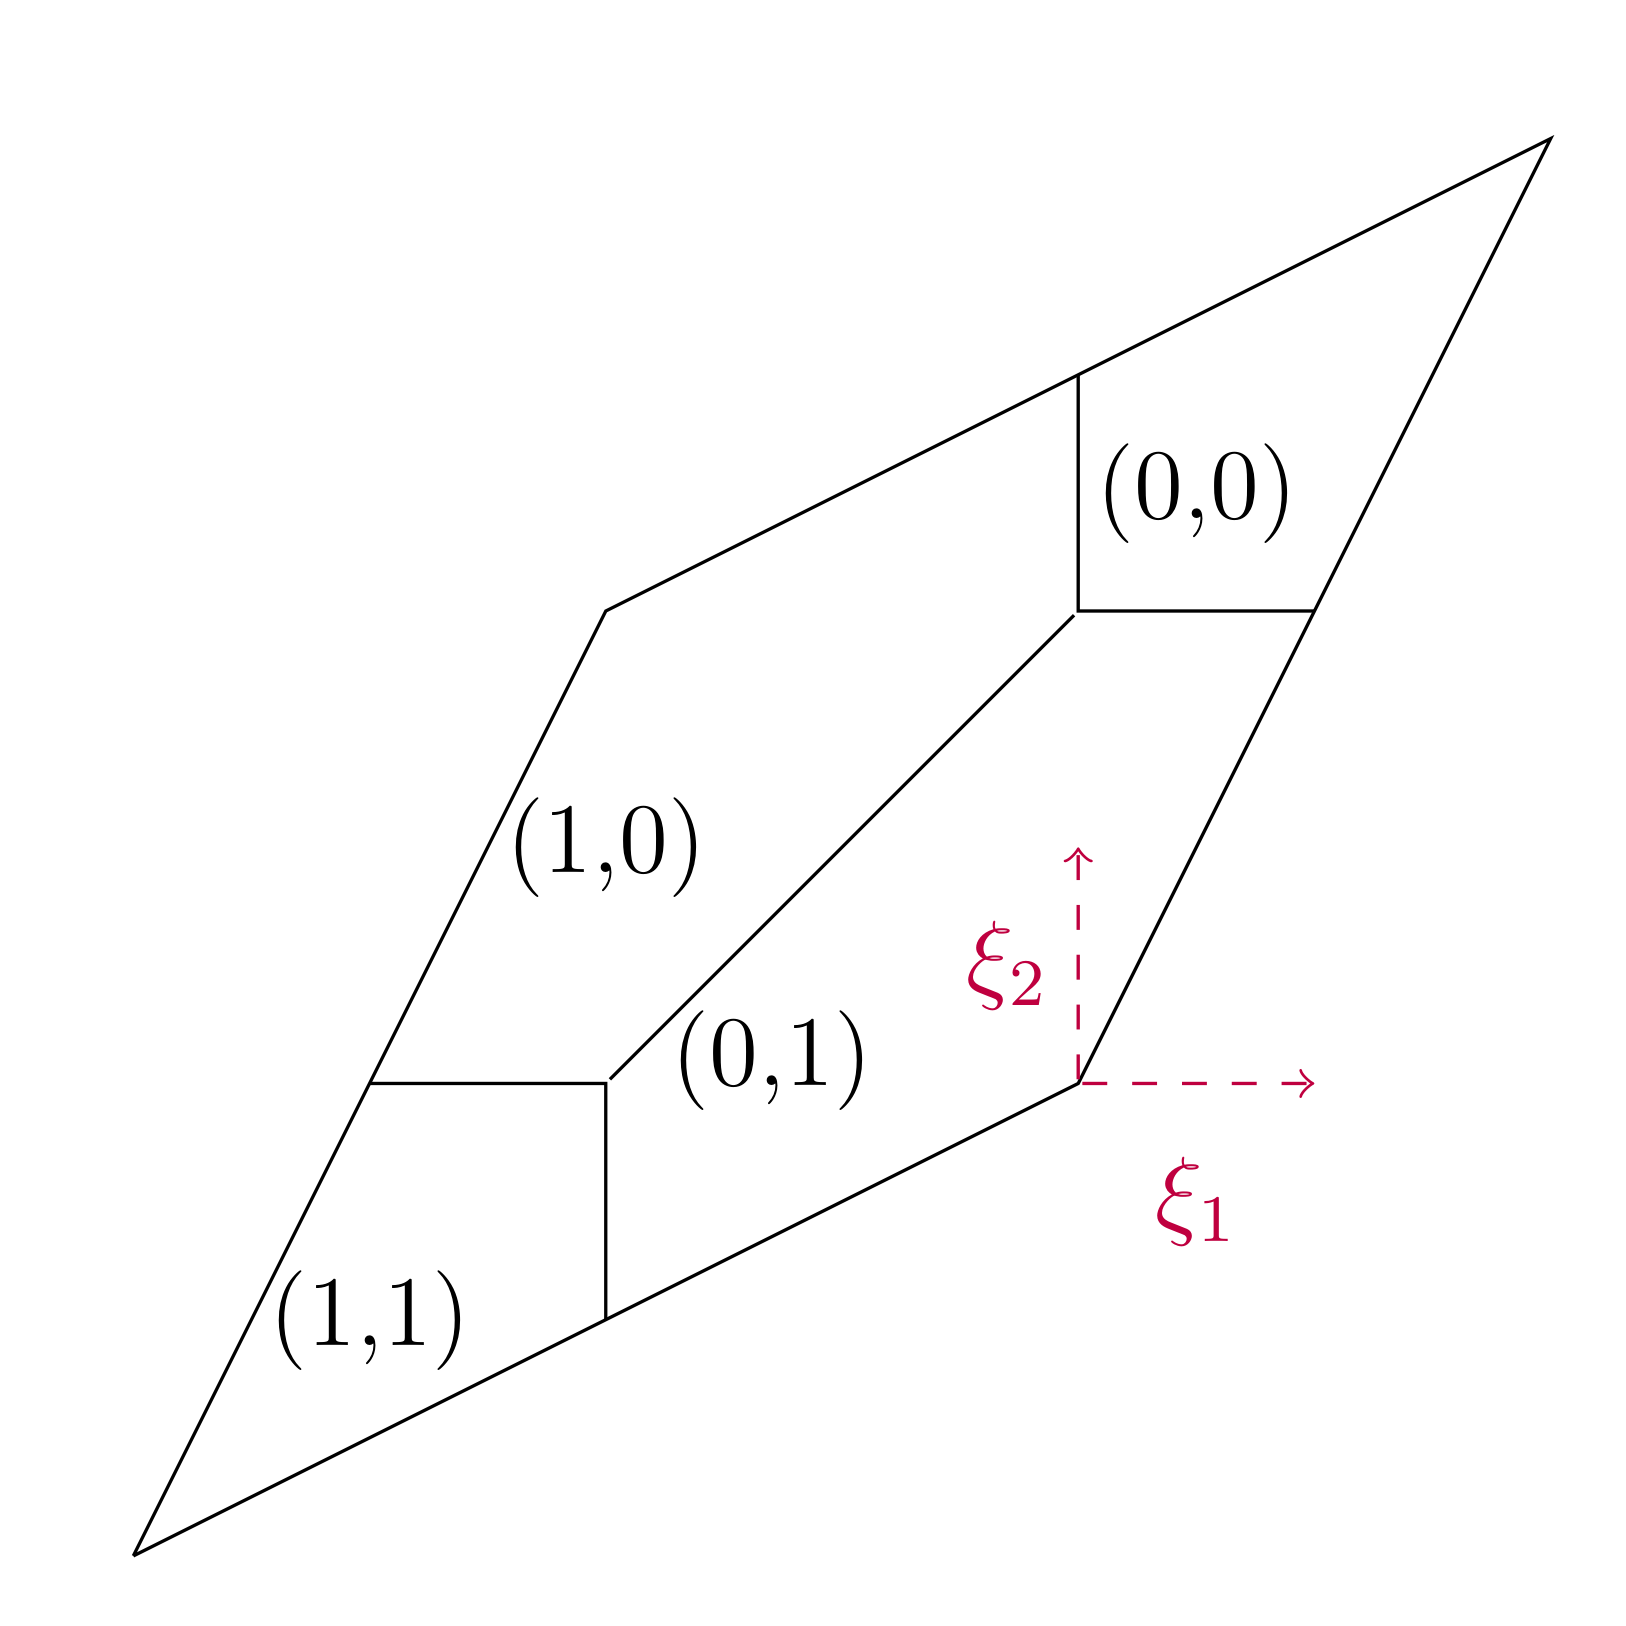
\includegraphics[width=0.40\textwidth]{figures/fig_4_1.png}
\caption{纤维中的单值性，看作平行四边形上的截面
$(\xi_1,\xi_2)\mapsto(\theta_1(\xi_1,\xi_2),\theta_2(\xi_1,\xi_2))$（原书 p.85）}
\label{fig:4-1}
\end{figure}

\begin{remark}[提醒]\label{rem:4-1-15}
下面定义由辛形式导出的作用--角坐标。我们将发现矩映射的像与环簇多面体
（toric polytope）相同，这是 Delzant 定理的一个实例，参见 [MS17]。注意通常的矩映射
落在 $\R^n$ 中（$n$ 为环面的维数），而这里的矩映射落在 $\R^3/\Gamma_B$ 中。
\end{remark}

\begin{claim}[作用--角坐标的定义]\label{clm:4-1-16}
令 $\theta_1:=\arg(x)$、$\theta_2:=\arg(y)$、$\theta_3=\arg(z)$，其中 $x,y,z$ 是复
环簇坐标。它们定义在如下区域中：$|v_0|=|xyz|\le T^\ell$（$\ell$ 充分大），并沿
$v_0\in\R_-$ 去掉一条分支割线；且 $x,y\in(\C^*)^2/\Gamma_B$。于是存在坐标
$\xi_1,\xi_2$ 使
\[
\restr{\omega}{\Vdual}=\de\xi_1\wedge\de\theta_1+\de\xi_2\wedge\de\theta_2,
\]
可简记为 $\de\xi\wedge\de\theta$。注意 $\xi_3,\theta_3$ 不是整体定义的，这正是需要
分支割线的原因。我们还有第三对坐标 $\eta$、$\theta_\eta:=\arg(v_0)$，其中
$\eta=\xi_1+\xi_2+\xi_3$。
\end{claim}

% [Tutor Note: 原书作 |v0|=|xyz| ≤ T^ℓ，其中 T 与 ℓ 的确切含义（阈值与幂次）未
% 说明；结合上下文应理解为 ℓ 充分大时的一个截断区域。保留原样并加译注。]

\begin{proof}
我们有局部 $T^3$-作用。由于 $\theta_i$ 已如上使用，这里改用符号 $\alpha_i$ 作坐标。
\[
\rho\colon T^3\times Y\to Y,\qquad
\rho((\alpha_1,\alpha_2,\alpha_3),(x,y,z))
=(e^{2\pi i\alpha_1}x,e^{2\pi i\alpha_2}y,e^{2\pi i\alpha_3}z).
\]
特别地，在坐标 $v_0$ 上这对应 $e^{2\pi i(\alpha_1+\alpha_2+\alpha_3)}v_0$。当 $v_0$
绕原点转满一圈时，$\theta_1,\theta_2$ 的值已按单值性改变，因此 $v_0$ 上的
$S^1$-作用不是整体定义的。这就是上面要沿割线去掉的原因。

$\alpha_1$ 与 $\alpha_2$ 在 $Y$ 上的无穷小作用由前推 $X_i:=\de\rho(\partial_{\alpha_i})$
（$i=1,2$）表示。若 $\iota_{X_i}\restr{\omega}{\Vdual}$ 是恰当的，比如等于某个函数
$H_i$ 的微分 $\de H_i$（$H_i$ 称为哈密顿量），则称该环面作用是\textbf{哈密顿群作用}
（Hamiltonian group action），而 $(H_1,H_2)$ 就是矩映射。这把我们引向
注~\ref{rem:4-1-15} 中的提醒。在当前设定中，$\omega$
% ===== 原书 p.86 =====
比较复杂，计算 $\iota_{X_i}\restr{\omega}{\Vdual}$ 并不容易。但我们知道：环面
$\R^4/\Lambda$（带 $\Lambda$-周期坐标 $a_1,a_2,a_3,a_4$）上的微分形式由
$\de a_1,\dots,\de a_4$ 在 $\C$ 上生成；由于 $a_i$ 不是整体定义的，这些形式不恰当。
因此存在 $\Gamma_B$-周期函数 $\xi_1,\xi_2$，使
\[
\begin{aligned}
\iota_{X_i}\restr{\omega}{\Vdual}&=\de\xi_i
\ \Longrightarrow\ \restr{\omega}{\Vdual}=\de\xi\wedge\de\theta\\
\Longrightarrow\quad
\iota_{X_i}\Big(\frac{i}{2\pi}\partial\bar\partial F\Big)
&=\frac{i}{2\pi}\de\iota_{X_i}\partial F=\de\xi_i\\
\therefore\quad \xi_1&:=\frac{i}{2\pi}\partial F(2\pi ix\partial_x)
=-\frac{1}{2}xe^{-i\theta_x}\frac{\partial F}{\partial|x|}\\
\therefore\quad \xi_1&=-\frac{1}{4}\frac{\partial F}{\partial|x|^2},
\qquad
\xi_2=-\frac{1}{4}\frac{\partial F}{\partial|y|^2}.
\end{aligned}
\]
其中用到 $\partial\bar\partial=-\bar\partial\partial=-\de\partial$、§2.2 的极坐标
换算，以及 $F$ 作为诸范数的函数在旋转 $x,y,z$ 下不变，故 Lie 导数
$\mathcal{L}_{X_i}\partial F=0$，且 $\partial_{\theta_x}F=0$。要点在于：矩映射
$(\xi_1,\xi_2)$ 给出周期的作用坐标，且由 $F$ 的定义方式，它们关于 $|x|$ 与 $|y|$
单调递增。（但请记住那条提醒：我们把它叫作矩映射，它取值于环面而非仿射空间，这里
是把矩映射的定义扩充到此情形。通常 $\xi_i$ 不应是周期的。）我们看到 $\Vdual$ 辛
同胚于 $(T^4,\omega_{std})$。

注意一条轨道恰为 $(\de\xi_1,\de\xi_2)$ 的核，故矩映射值的原像是一条 $T^2$-轨道。
换一种说法，环面作用保持矩映射。再换一种说法，矩映射纤维的切空间由
$\partial_{\theta_1},\partial_{\theta_2}$ 张成。

注意坐标 $(\xi_1,\xi_2,\eta)$ 以 $\xi\sim\xi+\gamma$ 与 $\eta\ge\varphi(\xi)$ 为周期，
而 $\varphi(\xi+\gamma)=\varphi(\xi)-\kappa(\gamma)+\ip{\xi}{\lambda(\gamma)}$，故当
$\gamma\in\Gamma_B$ 时 $\eta\sim\eta-\kappa(\gamma)+\ip{\xi}{\lambda(\gamma)}$。
\end{proof}

\transnote{$\xi_1,\xi_2$ 是周期的，这是本文「矩映射」一词的非标准之处：它取值于
$\R^3/\Gamma_B$ 而非 $\R^2$。提醒中的「扩充定义」即指此。}

\begin{corollary}\label{cor:4-1-17}
诸 $\ell_k$ 是纤维中的拉格朗日对象。
\end{corollary}

\begin{proof}
$\ell_k$ 是图 $\Gamma_{kM^{-1}(\xi)}$。于是
\[
T\ell_k=\big\langle\partial_{\xi_i}+kM^{-1}(\partial_{\theta_i})\big\rangle_{i=1,2},
\]
且
\[
\omega\big(\partial_{\xi_1}+kM^{-1}(\partial_{\theta_1}),
\partial_{\xi_2}+kM^{-1}(\partial_{\theta_2})\big)=0,
\]
因为 $\omega$ 只从 $\de\xi_1\wedge\de\theta_1$ 或 $\de\xi_2\wedge\de\theta_2$ 取项。
\end{proof}

\transnote{$T\ell_k$ 的两条切向量形如 $\partial_{\xi_i}+kM^{-1}(\partial_{\theta_i})$，
这是「$\ell_k$ 为 $\xi$ 上线性函数的图像」的微分表述：沿 $\xi_i$ 走一步，$\theta$
方向按斜率矩阵 $kM^{-1}$ 同步移动。}

\begin{remark}[记号]\label{rem:4-1-18}
$\mu_X$ 指最后一个坐标上的 $S^1$-作用。$\mu_Y$ 指局部 $T^3$-作用。
\end{remark}

\begin{claim}\label{clm:4-1-19}
（[AAK16]）函数 $\mu_X(x,y)$ 等于由 $(x,y)$ 的轨道所围的盘的面积。
\end{claim}

% ===== 原书 p.87 =====
\begin{proof}
我们断言 $\mu_X(x,y)=\int_D\omega$。这个盘上的积分（例如 $\PP^1$ 的矩映射像是线段，
可在该线段上画出拉长的球面，并把线段中的值映到球面中被扫过部分的面积）是沿如下盘
的积分：其边界分支为一条轨道（$X^{\#}$ 的积分流）以及从 $(x,y)$ 绕回原点的直线。
称该直线为 $C$。于是可把积分写成
\[
\int_C\iota_{X^{\#}}\omega=\int_C\de\mu_X=\mu_X(x,y)-\mu_X(0,0)=\mu_X(x,y).
\]
\end{proof}

\transnote{此处「盘的面积」按 $\PP^1$ 的矩映射像为线段来理解：线段上每个值对应球面
被扫过部分的面积，于是边界积分化为矩映射值之差。}

\begin{remark}\label{rem:4-1-20}
我们的出发点多面体，并希望它成为某个待构造辛形式下的矩映射像。特别地，我们要找
一个辛形式，使六边形的边界 $\PP^1$ 长度为 $1$。
\end{remark}

\medskip\noindent\textbf{单值性计算}\par
\begin{example}[降一维：二维局部情形]\label{ex:4-1-21}
$\C^2$ 带辛纤维丛 $(x,y)\mapsto xy$ 的情形即 Lefschetz 纤维丛的设定：奇异纤维由
$x=0$ 与 $y=0$ 给出的两份 $\C$ 构成，单值性是绕圆柱形纤维腰部 $S^1$ 的 Dehn 扭转。
Reference.
\end{example}

% [Tutor Note: 原书此处仅有「Reference.」一词，未给出具体文献，保留原样。]

\transnote{二维局部情形是 Lefschetz 纤维丛的标准图像：纤维是圆柱，奇异纤维为两份
$\C$ 沿原点粘合，单值性为绕腰部 $S^1$ 的 Dehn 扭转。下一例把这一图像逐坐标实现。}

$f(x,y)=xy$，$S^1$-作用为 $(e^{i\theta}x,e^{-i\theta}y)$。对应的全纯向量场是
$iz_1\partial_{z_1}-iz_2\partial_{z_2}$，它与
$\omega=\frac{i}{2}(\de z_1\wedge\de\bar z_1+\de z_2\wedge\de\bar z_2)$ 缩并给出
哈密顿向量场 $-\frac{1}{2}(|z_1|^2-|z_2|^2)$。我们在二维纤维上有一组新坐标：矩映射
坐标 $\mu$ 与作用的角坐标 $\theta$。当 $xy\to0$ 时，$\mu$-高度为 $0$ 的轨道，即
$|x|=|y|$ 处，趋于零。由此可以看出，为什么我们得到的是颈部收缩为零的圆柱图像。

\begin{example}[三维局部情形]\label{ex:4-1-22}
分几步来做。

\begin{itemize}[leftmargin=2.2em,itemsep=0.25em]
\item \textbf{全纯纤维丛的平行移动。} 设
\begin{equation}\label{eq:4-1}
\begin{aligned}
f&=xyz, & |f|^2&=(x_1^2+x_2^2)(y_1^2+y_2^2)(z_1^2+z_2^2)\\
\nabla_{\omega_0}f&=2\langle x|yz|^2,\;y|xz|^2,\;z|xy|^2\rangle\\
&\ \perp\ (|f|^2)^{-1}(c^2)=\{|xyz|=c\}
\end{aligned}
\end{equation}
于是 $|f|^2$ 的梯度向量场的投影与此情形中的圆垂直。特别地，乘以 $i$ 就得到与圆相切
的东西。乘以 $i$ 恰好给出正确的水平提升，这一点成立是因为 $f$ 全纯，从而与 $i$
交换。此外我们还会看到，梯度是水平子空间中元素的线性组合。

\transnote{这一步的三个算式各有分工：先求 $|f|^2$ 的梯度，它垂直于水平圆；乘 $i$
得切向；最后除以标量 $g$，使 $\de f(X_H)=iw\partial/\partial w$，从而 $X_H$ 覆盖
底空间中的圆。}

\item \textbf{求水平子空间。}
\begin{claim}\label{clm:4-1-23}
$X_{\Re(f)},X_{\Im(f)}\in H$，其中 $H$ 是水平分布。
\end{claim}

\begin{proof}
纤维恰为 $f$ 的水平集。
\begin{equation}\label{eq:4-2}
\begin{aligned}
\ker(d_pf)&=T_p(f^{-1}(c)),\qquad p\in f^{-1}(c)\\
\ker(\de f)&=\ker(\de\Re(f))\cap\ker(\de\Im(f))\\
\ker(\de\Re(f)(\cdot))&=\ker(\omega_0(X_{\Re(f)},\cdot))\ni X_{\Re(f)}\\
f\ \text{全纯}\ \Longrightarrow\ \nabla(\Re(f))&=-J\nabla(\Im(f))\\
\therefore\ \nabla(\Re(f))&=-JX_{\Re(f)}=X_{\Im(f)}
\ \Longrightarrow\ X_{\Im(f)}\in\ker(\de\Re(f))\\
\therefore\ H&=\big\langle X_{\Re(f)},X_{\Im(f)}\big\rangle
=\big\langle\nabla(\Re(f)),\nabla(\Im(f))\big\rangle
\end{aligned}
\end{equation}
\end{proof}

\item \textbf{平行移动的计算。} 把 $i$ 乘梯度作适当缩放后积分其水平提升，因为我们要
覆盖底空间中的圆。
\begin{equation}\label{eq:4-3}
\begin{aligned}
i\nabla(|f|^2)&=2i\langle\nabla\Re(f),\nabla\Im(f)\rangle\in Hor\\
&=2i\big\langle x_1|y|^2|z|^2,\;x_2|y|^2|z|^2,\;y_1|x|^2|z|^2,\;
y_2|x|^2|z|^2,\;z_1|x|^2|y|^2,\;z_2|x|^2|y|^2\big\rangle\\
\int_0^\theta i\nabla(|f|^2)&=\rho^{i\nabla(|f|^2)}(\theta)
=\big(e^{2i\theta|y|^2|z|^2}x,\;e^{2i\theta|x|^2|z|^2}y,\;
e^{2i\theta|x|^2|y|^2}z\big)
\end{aligned}
\end{equation}
\end{itemize}
\end{example}

% ===== 原书 p.88 =====
我们要找 $\frac{\partial}{\partial\theta}e^{i\theta}=iw\partial/\partial w$ 的水平提升。
即找一个适当的标量函数 $g$，使 $\de f(i(\nabla|f|^2)/g)=iw\partial/\partial w$。
\begin{align*}
\de f&=yz\,\de x+xz\,\de y+xy\,\de z\\
\nabla_{g_0}|f|^2&=2\langle x|yz|^2,\;y|xz|^2,\;z|xy|^2\rangle\\
|\nabla|f|^2|^2&=4|xyz|^2\big(|yz|^2+|xz|^2+|xy|^2\big)\\
\Longrightarrow\quad
\big(|yz|^2+|xz|^2+|xy|^2\big)&=\frac{|\nabla|f|^2|^2}{4|f|^2}\\
X_H&=\frac{2i}{g}\langle x|yz|^2,\;y|xz|^2,\;z|xy|^2\rangle
\quad\text{s.t.}\quad \de f(X_H)=iw\partial/\partial w\\
\therefore\quad
\frac{2i}{g}xyz\big(|yz|^2+|xz|^2+|xy|^2\big)&=iw=i(xyz)
\ \Longrightarrow\ g=2\big(|yz|^2+|xz|^2+|xy|^2\big)\\
\therefore\quad X_H&=\frac{i}{|yz|^2+|xz|^2+|xy|^2}
\langle x|yz|^2,\;y|xz|^2,\;z|xy|^2\rangle.
\end{align*}
于是
\begin{equation}\label{eq:4-4}
\begin{aligned}[b]
\therefore\quad \rho^{X_H}(x,y,z,\theta)
&=\Big(e^{i\theta\frac{|y|^2|z|^2}{|y|^2|z|^2+|x|^2|z|^2+|x|^2|y|^2}}x,\;
 e^{i\theta\frac{|x|^2|z|^2}{|y|^2|z|^2+|x|^2|z|^2+|x|^2|y|^2}}y,\\
&\qquad\qquad\qquad
 e^{i\theta\frac{|x|^2|y|^2}{|y|^2|z|^2+|x|^2|z|^2+|x|^2|y|^2}}z\Big)\\
&=\Big(e^{i\theta\frac{|x|^{-2}}{|x|^{-2}+|y|^{-2}+|z|^{-2}}}x,\;
 e^{i\theta\frac{|y|^{-2}}{|x|^{-2}+|y|^{-2}+|z|^{-2}}}y,\\
&\qquad\qquad\qquad
 e^{i\theta\frac{|z|^{-2}}{|x|^{-2}+|y|^{-2}+|z|^{-2}}}z\Big).
\end{aligned}
\end{equation}

% ===== 原书 p.89 =====
这里用到圆上 $w=xyz$，最后一步则除以 $|f|^2$，以便更容易看出 Dehn 扭转的行为。
这就给出本节开头的单值性结果，即引理~\ref{lem:4-1-11}。

\begin{example}[本文 $v_0\colon Y\to\C$ 的设定]\label{ex:4-1-24}
\end{example}

\begin{claim}\label{clm:4-1-25}
若 $\gamma(t)(v_0)=e^{2\pi it}v_0$，则 $\gamma'$ 的水平提升形如
\[
X_{hor}=\partial/\partial\theta_{v_0}+f(\xi)\partial/\partial\theta_1
+g(\xi)\partial/\partial\theta_2.
\]
\end{claim}

\begin{proof}
注意 $\operatorname{Lie}T^3$ 上的 Lie 括号为零，故标准理论给出
\[
\omega(X_{\zeta_1},X_{\zeta_2})=X_{[\zeta_1,\zeta_2]}=0.
\]
特别地，若取 $\zeta_1=(1,0,0)$ 或 $(0,1,0)$，即 $TF$ 的角切向（$F$ 为 $v_0$ 的
纤维），而 $\zeta_2$ 任意，则得零。又因 $\omega(X_{(1,0,0)},-)=\de\xi_1$，可见
$X_{\zeta_2}$ 不含 $\partial/\partial\xi_1$ 分量；换言之，它的流保持矩映射坐标
$\xi_1$ 与 $\xi_2$。

特别地，设 $X_{hor}$ 为断言中的水平提升。设 $X_{(1,0,0)}$ 为旋转 $x$ 坐标（保持
$y$ 与 $v_0$ 不动）的无穷小作用生成的向量场。于是 $X_{hor}$ 的水平性（按矩映射
$\xi_1$ 的定义）给出
\[
\de\xi_1(X_{hor})=\omega(X_{(1,0,0)},X_{hor})=0.
\]
因此若 $\phi_t$ 是 $X_{hor}$ 的流，由链式法则得
\[
\frac{\de}{\de t}(\xi_1\circ\phi_t)=0
\qquad\therefore\quad \xi_1\circ\phi_t=\xi_1,
\]
对 $\xi_2$ 同理。故平行移动保持矩映射坐标 $\xi_1,\xi_2$。它还保持 $\eta$，因为我们
考虑的是角向平行移动。于是在坐标
$\pi\colon(\xi_1,\xi_2,\eta,\theta_x,\theta_y,\theta_{v_0})\to(|w|,\theta_w)
:=(|v_0|,\theta_{v_0})$ 下（$w$ 为 $v_0\colon Y\to\C$ 底空间 $\C$ 上的坐标），
\[
\de\pi(X_{hor})=\partial/\partial\theta_{v_0}
\]
\[
\Longrightarrow\quad
\begin{pmatrix}
0&0&\partial|v_0|/\partial\eta&0&0&0\\
0&0&0&0&0&1
\end{pmatrix}
\begin{pmatrix}0\\0\\h\\f\\g\\a\end{pmatrix}
=\begin{pmatrix}h\,\partial|v_0|/\partial\eta\\ a\end{pmatrix}=(0,1),
\]
故 $a=1$、$h=0$，因为 $\eta$ 依赖于 $|v_0|$。于是水平提升取如下形式：
\[
X_{hor}=\partial/\partial\theta_{v_0}+f\partial/\partial\theta_1
+g\partial/\partial\theta_2.
\]
\end{proof}

% ===== 原书 p.90 =====
\begin{corollary}\label{cor:4-1-26}
$X_{hor}=\partial/\partial\theta_{v_0}+f\partial/\partial\theta_1
+g\partial/\partial\theta_2$，其中 $f$ 与 $g$ 只是 $\xi_1,\xi_2$ 的函数。
\end{corollary}

\begin{proof}
注意：由矩映射在径向平行移动下的不变性，可得与 $\eta$ 无关。设 $\rho^t$ 为来自
角向平行移动的水平向量场 $X_{hor}$ 的流：
\[
\rho^t(\xi_1,\xi_2,\eta,\theta_1,\theta_2,\theta_{v_0})
=(\xi_1,\xi_2,\eta,\theta_1+tf,\theta_2+tg,\theta_{v_0}+t).
\]
设 $\phi_\alpha$ 为 $T^2$-作用 $(e^{2\pi i\alpha_1}x,e^{2\pi i\alpha_2}y,v_0)$。它是
辛同胚：因为全纯且保持诸范数，故与 $\partial\bar\partial$ 交换并保持凯勒势 $F$，从而
$(\phi_\alpha)_*\partial\bar\partial F=\partial\bar\partial F$。它还是逐纤维的辛同胚，
因为它在纤维上作用。于是
\begin{align*}
0&=\phi_\alpha^*\omega(TF,H)=\omega((\phi_\alpha)_*TF,(\phi_\alpha)_*H)\\
&=\omega(TF,(\phi_\alpha)_*H)\\
&\qquad\therefore\quad (\phi_\alpha)_*H=H\\
\de\pi((\phi_\alpha)_*X_{hor})&=\de(\pi\circ\phi_\alpha)(X_{hor})=\de\pi(X_{hor})\\
&\qquad\therefore\quad (\phi_\alpha)_*(X_{hor})\circ\phi_\alpha^{-1}=X_{hor}\\
\Longrightarrow\quad \de\phi_\alpha\Big(\frac{\de}{\de t}\rho^t\Big)\circ\phi_\alpha^{-1}
&=\frac{\de}{\de t}(\phi_\alpha\circ\rho^t)\circ\phi_\alpha^{-1}\\
&=\frac{\de}{\de t}(\rho^t)\\
\Longrightarrow\quad \phi_\alpha\circ\rho^t&=\rho^t\circ\phi_\alpha\\
\Longrightarrow\quad
&(\xi_1,\xi_2,\eta,\theta_1+\alpha_1+tf(\xi,\theta+\alpha),\\
&\qquad \theta_2+\alpha_2+tg(\xi,\theta+\alpha),\theta_{v_0}+t)\\
&=
(\xi_1,\xi_2,\eta,\theta_1+\alpha_1+tf(\xi,\theta),\\
&\qquad \theta_2+\alpha_2+tg(\xi,\theta),\theta_{v_0}+t)\\
\Longrightarrow\quad f(\xi,\theta+\alpha)=f(\xi,\theta),\quad
g(\xi,\theta+\alpha)&=g(\xi,\theta)\quad\forall\alpha
\end{align*}
其中我们沿 $\frac{\de}{\de t}$ 积分得到下一行。于是 $f$ 与 $g$ 与 $\theta_1,\theta_2$
无关。类似的论证表明它们也与 $\theta_{v_0}$ 无关，即对 $v_0$ 坐标上的 $S^1$-作用
$\phi_\lambda$（$\lambda\in S^1$）有 $\phi_\lambda\circ\rho^t=\rho^t\circ\phi_\lambda$。
\end{proof}

\medskip\noindent\textbf{与线性拉格朗日哈密顿同痕的纤维拉格朗日}\par
\begin{definition}\label{def:4-1-27}
令 $L_i$ 为纤维中 $\ell_i$ 沿 U 形曲线的平行移动。
\end{definition}

\begin{claim}\label{clm:4-1-28}
平行移动后的 $\ell_i$ 与 $\ell_{i+1}$ 哈密顿同痕。
\end{claim}

\begin{proof}
我们在纤维中构造同痕 $\psi_t\colon F\to F$（坐标 $(\xi_1,\xi_2,\theta_1,\theta_2)$）。
它把 $\ell_1$ 映到 $\phi(\ell_0)$，其中 $\phi$ 是单值性。为证 $\psi_t$ 是哈密顿
同痕，即 $\iota_{\frac{\de}{\de t}\psi_t}\omega=\de H_t$ 对某 $H_t$ 成立，Banyaga
的结果（参见 Pascaleff 讲义）表明只须证明：$\omega$ 经由 $H_1(F)$ 的生成元扫出的
圆柱的通量为零。
\[
\Big\langle\int_t\iota_{X_t}\omega,[\gamma]\Big\rangle
=\ip{\operatorname{Flux}(\psi_t)}{[\gamma]}
=\int_{\psi_t(\gamma)}\omega
=\text{$\gamma$ 随时间扫出的圆柱的面积}.
\]
% ===== 原书 p.91 上部（§4.1 收尾；§4.2 起属下块） =====
先定义同痕，并令 $A:=M^{-1}$。
\[
\psi_t(\xi_1,\xi_2,\theta_1,\theta_2)
:=(\xi_1,\xi_2,\theta_1+t(f(\xi)-A_1\xi),\theta_2+t(g(\xi)-A_2\xi)).
\]

\transnote{减去 $A\xi$ 是为了去掉线性拉格朗日 $\ell_1$ 自身的斜率：$A=M^{-1}$ 正是
该斜率矩阵，故 $\psi_t$ 从恒等出发，在 $t=1$ 时把线性图拉成平行移动后的图。}
注意 $H_1(F)$ 的秩为四，因为 $F\iso T_B\times T_F$。若取 $\gamma$ 为
$(0,0,1,0)$ 或 $(0,0,0,1)$ 生成的两个角向中的回路，则 $\{\psi_t(\gamma)\}_t$ 是一维
的，因为 $\xi$ 为常数，故积分为零。今取
\[
\gamma(t)=(2t,t,0,0),\qquad -\frac{1}{2}\le t\le\frac{1}{2}.
\]
$\gamma(t)=(t,2t,0,0)$ 的情形类似。
\begin{align*}
\operatorname{flux}&=\int_{\psi_t(\gamma)}\omega=\int_\gamma\iota_{X_t}\omega
=\int_\gamma(\de\xi_1\wedge\de\theta_1+\de\xi_2\wedge\de\theta_2)
\big((f-A_1)\partial_{\theta_1}+(g-A_2)\partial_{\theta_2},-\big)\\
&=\int_\gamma(f-A_1)\de\xi_1+(g-A_2)\de\xi_2
=\int_{-1/2}^{1/2}2f(2t,t)\,\de t+g(2t,t)\,\de t,
\end{align*}
其中用到 $A$ 是线性映射这一事实所蕴含的关于零点的对称性；剩下要证上式为零，即
$f$ 与 $g$ 关于零点的对称性。只须证明 $f(-\xi)=-f(\xi)$，对 $g$ 同理。

为此回忆 $f$ 与 $g$ 由
\[
X_{hor}=\frac{\partial}{\partial\theta_{v_0}}
+f(\xi)\frac{\partial}{\partial\theta_1}
+g(\xi)\frac{\partial}{\partial\theta_2}
\]
定义。也回忆 $X_{hor}$ 被任何保纤维的辛同胚保持，正如上面 $T^2$-作用的例子所示。
另一个保纤维的辛同胚是纤维中的
$\phi_{neg}\colon(\xi,\theta)\mapsto(-\xi,-\theta)$。它是辛同胚，因为
$\de\xi\wedge\de\theta\mapsto\de(-\xi)\wedge\de(-\theta)=\de\xi\wedge\de\theta$。
于是
\[
(\phi_{neg})_*(X_{hor})=X_{hor}\circ\phi_{neg}
\qquad\Longrightarrow\quad f(-\xi)=-f(\xi),\quad g(-\xi)=-g(\xi).
\]
这就完成了证明。
\end{proof}

\transnote{「通量为零」是同痕可写成哈密顿流的判据（Banyaga 定理），本文只须对
$H_1(F)$ 的生成元验证。末尾的 $\phi_{neg}$ 论证把 $f,g$ 的对称性化归为 $X_{hor}$
在保纤维辛同胚下的不变性。}

% EN48 c07 | 原书 p.91 中部–110 上部（PDF 100–119） | 第 4 章 §4.2–4.3
% 块边界：p.91 上半属 §4.1 证明收尾（归 c06）；p.110 下半起为 §4.4（归 c08）。
\subsection{定义 $H^0(\mathrm{FS}(Y,v_0))$ 的背景}

% ===== 原书 p.91 =====

以下背景取自 [Sei08]。

% ===== 原书 p.92 =====

\begin{figure}[htbp]
\centering
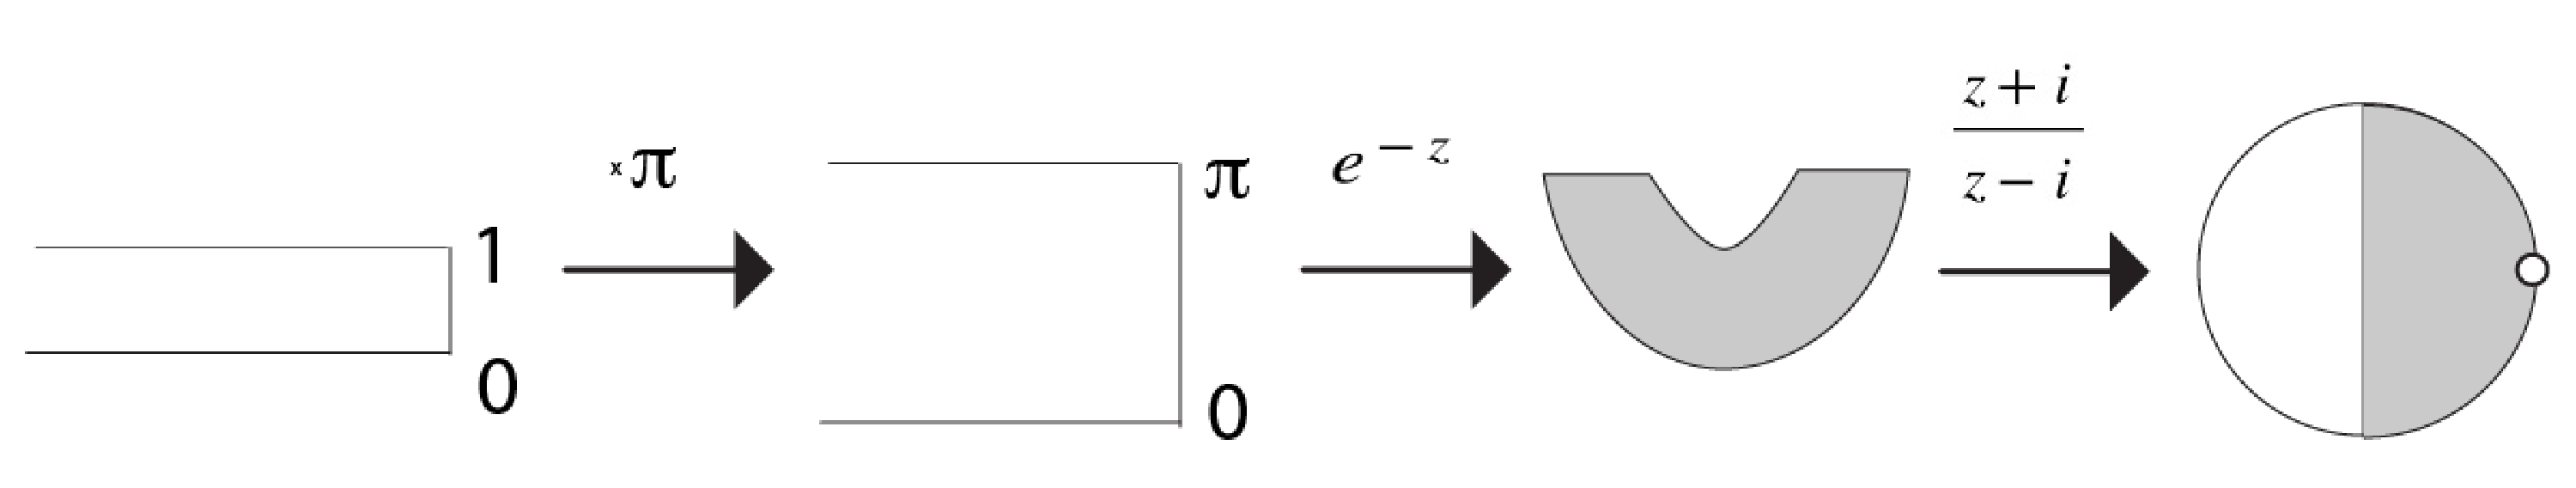
\includegraphics[width=0.8\textwidth]{figures/fig_4_2.png}
\caption{条状端的例子（原书 p.92）}
\label{c7:fig-strip-end}
\end{figure}

\begin{remark}[记号]\label{c7:rem-notation}
我们从辛纤维丛 $v_0\colon Y\to\C$ 讲起。它不是正合的，因为纤维是紧环面。
$Y$ 本身没有边界；不过下文会限制到原点附近的一个小圆盘，那里有边界。
按 [Sei08] 的术语，纤维是环面，所以没有水平边界；但取底空间中一个紧邻域的原像，就得到竖直边界。

我们考虑的近复结构满足两条：1）与上面定义的 $\omega$ 相容；2）在边界附近等于由复环面坐标诱导的标准结构 $J_0$。
这个集合记作 $\cJ_{\mathrm{reg}}(Y,\partial Y)$。它非空，因为含 $J_0$；它又可缩，论证与「全体 $\omega$-相容近复结构之集可缩」相同。
\end{remark}

\transnote{「水平边界 / 竖直边界」是 [Sei08] 的术语：水平边界指纤维方向的边界，竖直边界指底空间方向的边界。这里纤维是闭环面，没有水平边界；把底空间截成圆盘，才出现竖直边界。后文说「边界附近取 $J_0$」，指的是这个竖直边界。}

\begin{definition}[区域]\label{c7:def-domains}
带 puncture 的边界黎曼面 $S$，指这样一组数据：一个紧、连通、带边且边界非空的黎曼面，在其边界上挖去若干 puncture；再给 $\partial S$ 的每个连通分支指定一个正合拉格朗日。

我们再给 $S$ 加一层额外结构，称为「刚性化」。把 puncture 分为「正」「负」两类，并分别用嵌入
\[
\eps\colon(-\infty,0]_s\times[0,1]_t\to D,
\qquad
\eps\colon[0,\infty)_s\times[0,1]_t\to D
\]
定义负、正 puncture $\zeta^\pm$ 处的条状端，要求 $\lim_{s\to\pm\infty}\eps(s,t)=\zeta^\pm$。
这样的 $S$ 叫作带条状端的黎曼面。
\end{definition}

\begin{example}\label{c7:ex-strip-end}
本文中 $S$ 只会是三种情形之一：单位圆盘 $D$；两个圆盘沿边界上一点粘起来；一个圆盘与一族球之并。每种情形都可能带若干 puncture。

后文用来粘接两个圆盘的一个条状端是
\[
(-\infty,0]\times[0,1]\ni(s,t)
\mapsto
\eps_-(s,t):=\frac{e^{-\pi(s+it)}+i}{e^{-\pi(s+it)}-i}
=\frac{z+i}{z-i}\circ e^{-z}\circ\pi\cdot(s+it)\in D\setminus\{1\}.
\]
注意 $-\infty$ 就是该 puncture，它在圆盘中映到 $\zeta^-:=1$。见图~\ref{c7:fig-strip-end}。
\end{example}

\transnote{公式里的复合次序由图~\ref{c7:fig-strip-end} 读出：条带先经 $\pi$ 变成一条宽度为 $\pi$ 的方块，再经 $e^{-z}$ 变成下半圆环，最后经 $(z+i)/(z-i)$ 变成单位圆盘。原文没有单独定义 $\pi$，它的作用是把 $(-\infty,0]\times[0,1]$ 解释成标准方块坐标 $(-\infty,0]\times[0,\pi]$；照图理解即可。}

\begin{remark}\label{c7:rem-rigidify}
之所以叫「刚性化」，是因为对 $S$ 的任何操作都必须保持条状端这层额外数据，限制因此更严。
条带在 puncture 附近给出一组好坐标（即 $s$ 与 $t$），于是把两个截面沿 $(s,t)$ 坐标线性粘接，就是一种直接的做法。
参看 [Sei08, §(8i) 与 §(9k)]。
\end{remark}

\begin{definition}[映射]\label{c7:def-maps}
设 $J\in\cJ_{\mathrm{reg}}(Y,\partial Y)$。伪全纯映射指 $J$-全纯映射
\[
u\colon(S,\partial S)\to\Bigl(Y,\bigsqcup_{i\in\pi_0(\partial S)}L_i\Bigr).
\]
$J$-全纯曲线（伪全纯曲线）指这种映射的像。此外要求：对趋于 $L_i\cap L_j$ 中交点的条状端 $\eps_{ij}$，有
\begin{equation*}
\lim_{s\to\pm\infty}u(\eps_{ij}(s,t))\in L_i\cap L_j .
\end{equation*}
\end{definition}

\transnote{这里的极限条件就是「曲线的边界跑到两个拉格朗日的交点上」。$L_i$ 是 $\partial S$ 第 $i$ 个分支对应的拉格朗日。一个条状端只有一个极限方向：正 puncture 取 $s\to+\infty$，负 puncture 取 $s\to-\infty$。puncture 两侧的边界条件来自条状端的两条边 $t=0$ 与 $t=1$，它们分别映到 $L_i$ 与 $L_j$，故极限点必须同时在 $L_i$ 与 $L_j$ 中。}

\begin{remark}[有了辛纤维丛的数据，可以看截面]\label{c7:rem-sections}
上面这些可以看作某个平凡纤维丛的截面，边界条件固定为拉格朗日。现在推广到非平凡纤维丛。
在纤维丛的全空间里考虑全纯多边形，其边界落在「沿底空间中该多边形平行移动」所得的纤维拉格朗日里。
把它投影到底空间，得到的是全纯多边形。这提示我们应当看全纯截面。
\end{remark}

\begin{definition}[截面]\label{c7:def-sections}
伪全纯截面可以类似地定义。它的极限不再是横截拉格朗日的交点，而是一个函数 $u_\zeta(t)$。
对每个 $t$，这个函数给出 $M$ 中一个可能随 $t$ 变化的点；它满足适当的导数条件，并在 $\partial S$ 上落在两个拉格朗日边界条件的交叠处。
% [Tutor Note: 原文此处 M 未定义，疑指纤维；保留原符号，译文照录。]
\end{definition}

\begin{remark}\label{c7:rem-nontransverse}
上面的讨论假设拉格朗日横截相交。拉格朗日是半维的；横截相交时其交为 $0$ 维，是一离散点集。

处理非横截相交，文献中已有几种办法。一种是引入 Hamilton 函数，沿与该函数微分辛对偶的向量场推动其中一个拉格朗日，直到两者横截相交。
[Sei08] 用的就是这一种。这个操作可以在纤维丛的纤维上做，所以我们在此交代背景。

给定定义在纤维上的 Hamilton 函数 $H$，以及定义在 $v_0$ 的底空间上、在边界上为零的 $1$-形式 $\gamma$。
具体地，在没有问题的 puncture 附近取 $\gamma=0$；在两个拉格朗日不横截相交的 puncture 附近取 $\gamma\neq0$。
此时映射 $u$ 应满足修正的 Cauchy--Riemann 方程
\begin{equation*}
(\de u-X_H\circ\gamma)^{0,1}=0,
\end{equation*}
并在条状端上取修正的边界条件。等价地说，$u$ 的极限落在「该拉格朗日」与「另一与之非横截相交的拉格朗日在 $X_H$ 的 time-$1$ 流下之像」的交点上。
用这一套可以计算纤维中拉格朗日 $\ell_i$ 的自同态。

在全空间上则必须换一种扰动方法，因为辛形式不是底空间与纤维的乘积。我们改用 [AS] 的范畴局部化方法，后文再说。
\end{remark}

\transnote{$X_H$ 定义在纤维上，$\gamma$ 定义在底空间上；$X_H\circ\gamma$ 不能按字面直接复合。对截面 $u$ 应这样读：先用 $\gamma$ 把底空间中的点送到 $H$ 的参数，再取该处的竖直向量场。原文写法简略，读者不要被符号骗到。}

\begin{example}\label{c7:ex-tz}
设 $t_z$ 是矩映射值 $(c_1,c_2)\in T_B$ 的原像与某个纤维之交。于是
\[
t_z=\{(c_1,c_2,\theta_1,\theta_2)\}_{\theta_i\in[0,2\pi)} .
\]
它对平行移动不变，因为平行移动只是转动角度。
$\ell_i\cap t_z$ 是 $\ell_i$ 中满足 $(\xi_1,\xi_2)=(c_1,c_2)$ 的唯一点，所以任何伪全纯截面 $u$ 在该 puncture 上方必极限到这一点。
\end{example}

% ===== 原书 p.94 =====

\begin{example}\label{c7:ex-tz-self}
$t_z\cap t_z$ 的交不横截，所以要像上面那样引入非齐次 Hamilton 项。
它是纤维上的光滑函数（在纤维边界附近为零；环面没有边界，这一条不必操心）。
本例中 $X_H$ 的 time-$1$ 流是纤维的一个自同构，它是坐标实范数 $|x|,|y|,|z|$ 上的图，并选得可以下降为环面到自身的映射。
由 PSS 同构，$\mathrm{HF}^*(t_z,t_z)\cong H^*(t_z;\C)$，即 $2$-环面的上同调。
\end{example}

\transnote{这里能算出 $\mathrm{HF}^*(t_z,t_z)$，关键在 $t_z$ 是矩映射的一个纤维——它是 $2$-环面，且被 Hamilton 项推成的自映射可以下降为环面到自身的映射。PSS 同构把 Floer 同调与奇异上同调接起来，故右端是 $H^*(T^2;\C)$。}

\subsection{定义 $H^0(\mathrm{FS}(Y,v_0))$ 所需的模空间}

% ===== 原书 p.94 =====

\begin{remark}[深谷范畴里为何需要模空间]\label{c7:rem-moduli-reason}
深谷范畴是 $A_\infty$-范畴。意思是：它有对象、态射，以及对任意自然数 $k$ 的「$k$ 个态射上的结构映射」。
这些映射满足 $A_\infty$ 关系；可以把 $A_\infty$ 关系看成态射的高阶结合律。

对象是拉格朗日，态射是交点，结构映射数的是带边界 puncture 的伪全纯映射：这些 puncture 极限到 $k$ 个输入交点与 $1$ 个输出交点。
对 Fukaya--Seidel 范畴，输入换成辛纤维丛，上面的「映射」相应换成「截面」。

为了真能数清楚，先把映射收进一个集合，再对重参数化取商。Gromov 给这个商集配了拓扑，使之成为拓扑空间。
由于我们模掉了黎曼面 $S$ 的自同构，这个空间称为模空间。
他的 Gromov 紧性定理把这个拓扑空间紧化：办法是分析伪全纯曲线的极限可能出现哪些行为。
所用复分析结论（如唯一延拓、某处单射性）在伪全纯情形依然成立。

不过要数数，我们希望得到紧的 $0$ 维流形。于是用函数空间上的微分几何，给模空间安上「紧 $0$ 维光滑流形」的结构；这样它就化成一个可数的有限数。
下面是我们计划：先定义模空间，再把它们装进 Fukaya--Seidel 范畴的框架，最后完成 HMS 计算。

\begin{itemize}[leftmargin=1.6em,itemsep=0.2em]
\item 紧接着：确定曲线映到 $Y$ 中的哪些同调类。
\item 本节（§4.3）：证明正则 $J$ 存在，使深谷范畴中的模空间是紧 $0$ 维流形。
      这一步把 [MS12] 从 $S=\PP^1$ 的情形改写到 $S=D$、带拉格朗日边界条件的情形；[Sei08] 与 [Gan16b] 也有讨论。
% ===== 原书 p.95 =====
\item §4.4：按 [AS] 定义范畴，并用标准的连续映射论证证明：它不依赖正则 $J$ 的选择，也不依赖 $FS(Y,v_0)$ 中拉格朗日的 Hamilton 同痕类；到拟同构为止唯一。
\item 第 8 章：算出对象、态射、微分与复合，找出 $H^0(FS(Y,v_0))$ 的一个子范畴，并证明它与镜像上有界相干层导出范畴同构。
      这里需要真的数出模空间，而非只知道计数存在；为此要用非正则 $J$ 与 Gromov--Witten 理论的结果 [KL19]。
      抽象正则化理论把定义与计算接起来，见 §5.1。
\end{itemize}

后三步都牵涉模空间。图~\ref{c7:fig-flow} 是一张流程图，说明如何定义模空间、以及打算拿它们做什么。
\end{remark}

\transnote{本图按原图裁入，没有重绘；框内英文是原书的流程标签，保留不动。读法：右列六个框是「选同调类 $\beta$、选 $J$、取映射集、商掉 $\Aut$、配 Gromov 拓扑、Gromov 紧化」，
左框是所得紧模空间，中框是「数这些模空间才能定义 $A_\infty$ 结构映射」，底部两条路是几何正则化与抽象正则化。}

\begin{lemma}[$Y$ 的同调]\label{c7:lem-homology-Y}
\[
H_2(Y)\cong H_2(\C\PP^2(3)/\Gamma_B)\cong\Z^4,
\]
其中同调类都取 $\Z$ 系数。
\end{lemma}

\begin{proof}
注意 $Y$ 形变收缩到可缩底空间上的中心纤维，故 $Y$ 的同调就是中心纤维的同调。

把中心纤维看成 $T^4$ 纤维退化所得，于是可通过「胞腔分解里什么缩成一点」来算同调。
我们想要低一维情形的类比：$T^2$ 退化为两端粘在一起的球。
从环面看成正方形的商可见此：一对对边缩成一点。或用胞腔分解说：从 $1$ 个 $0$-胞腔、$2$ 个 $1$-胞腔、$1$ 个绕两圆束的 $2$-胞腔构造 $2$-环面时，缩掉其中一条 $1$-胞腔。

图~\ref{c7:fig-2skeleton} 想画出 $T^4$ 胞腔构造的 $2$-骨架，即把 $T^4$ 看成 $4$-立方体的商。
我们得到三个 $2$-环面，它们在一个 $S^1$ 处粘起来。算二阶同调只需 $2$-骨架，故同调是 $\Z^3$，每个 $T^2$ 贡献一个生成元。
退化到中心纤维时，这个 $S^1$ 缩成一点，得到带三个香蕉球的香蕉流形；回忆一下，它就是六边形给出的中心纤维的边界。
$S^1$ 缩点后多出一个生成元，故同调为 $\Z^4$。
注意纤维实际是 $T_B\times T_F$ 而非 $I^4$，但两者拓扑相同。
\end{proof}

\transnote{「香蕉流形」不是标准术语，是作者对三个球在同一点相粘所得空间的俗称（补一句译者按：[CLS11] 的环簇语言里，它是三次爆破后的中心纤维；此句原书未写）。
「每个 $T^2$ 贡献一个生成元」指的是 $H_2$ 的三个 $\Z$ 生成元，不是说每个 $T^2$ 的同调是 $\Z^3$。}

% ===== 原书 p.96 =====

\begin{figure}[tbp]
\centering
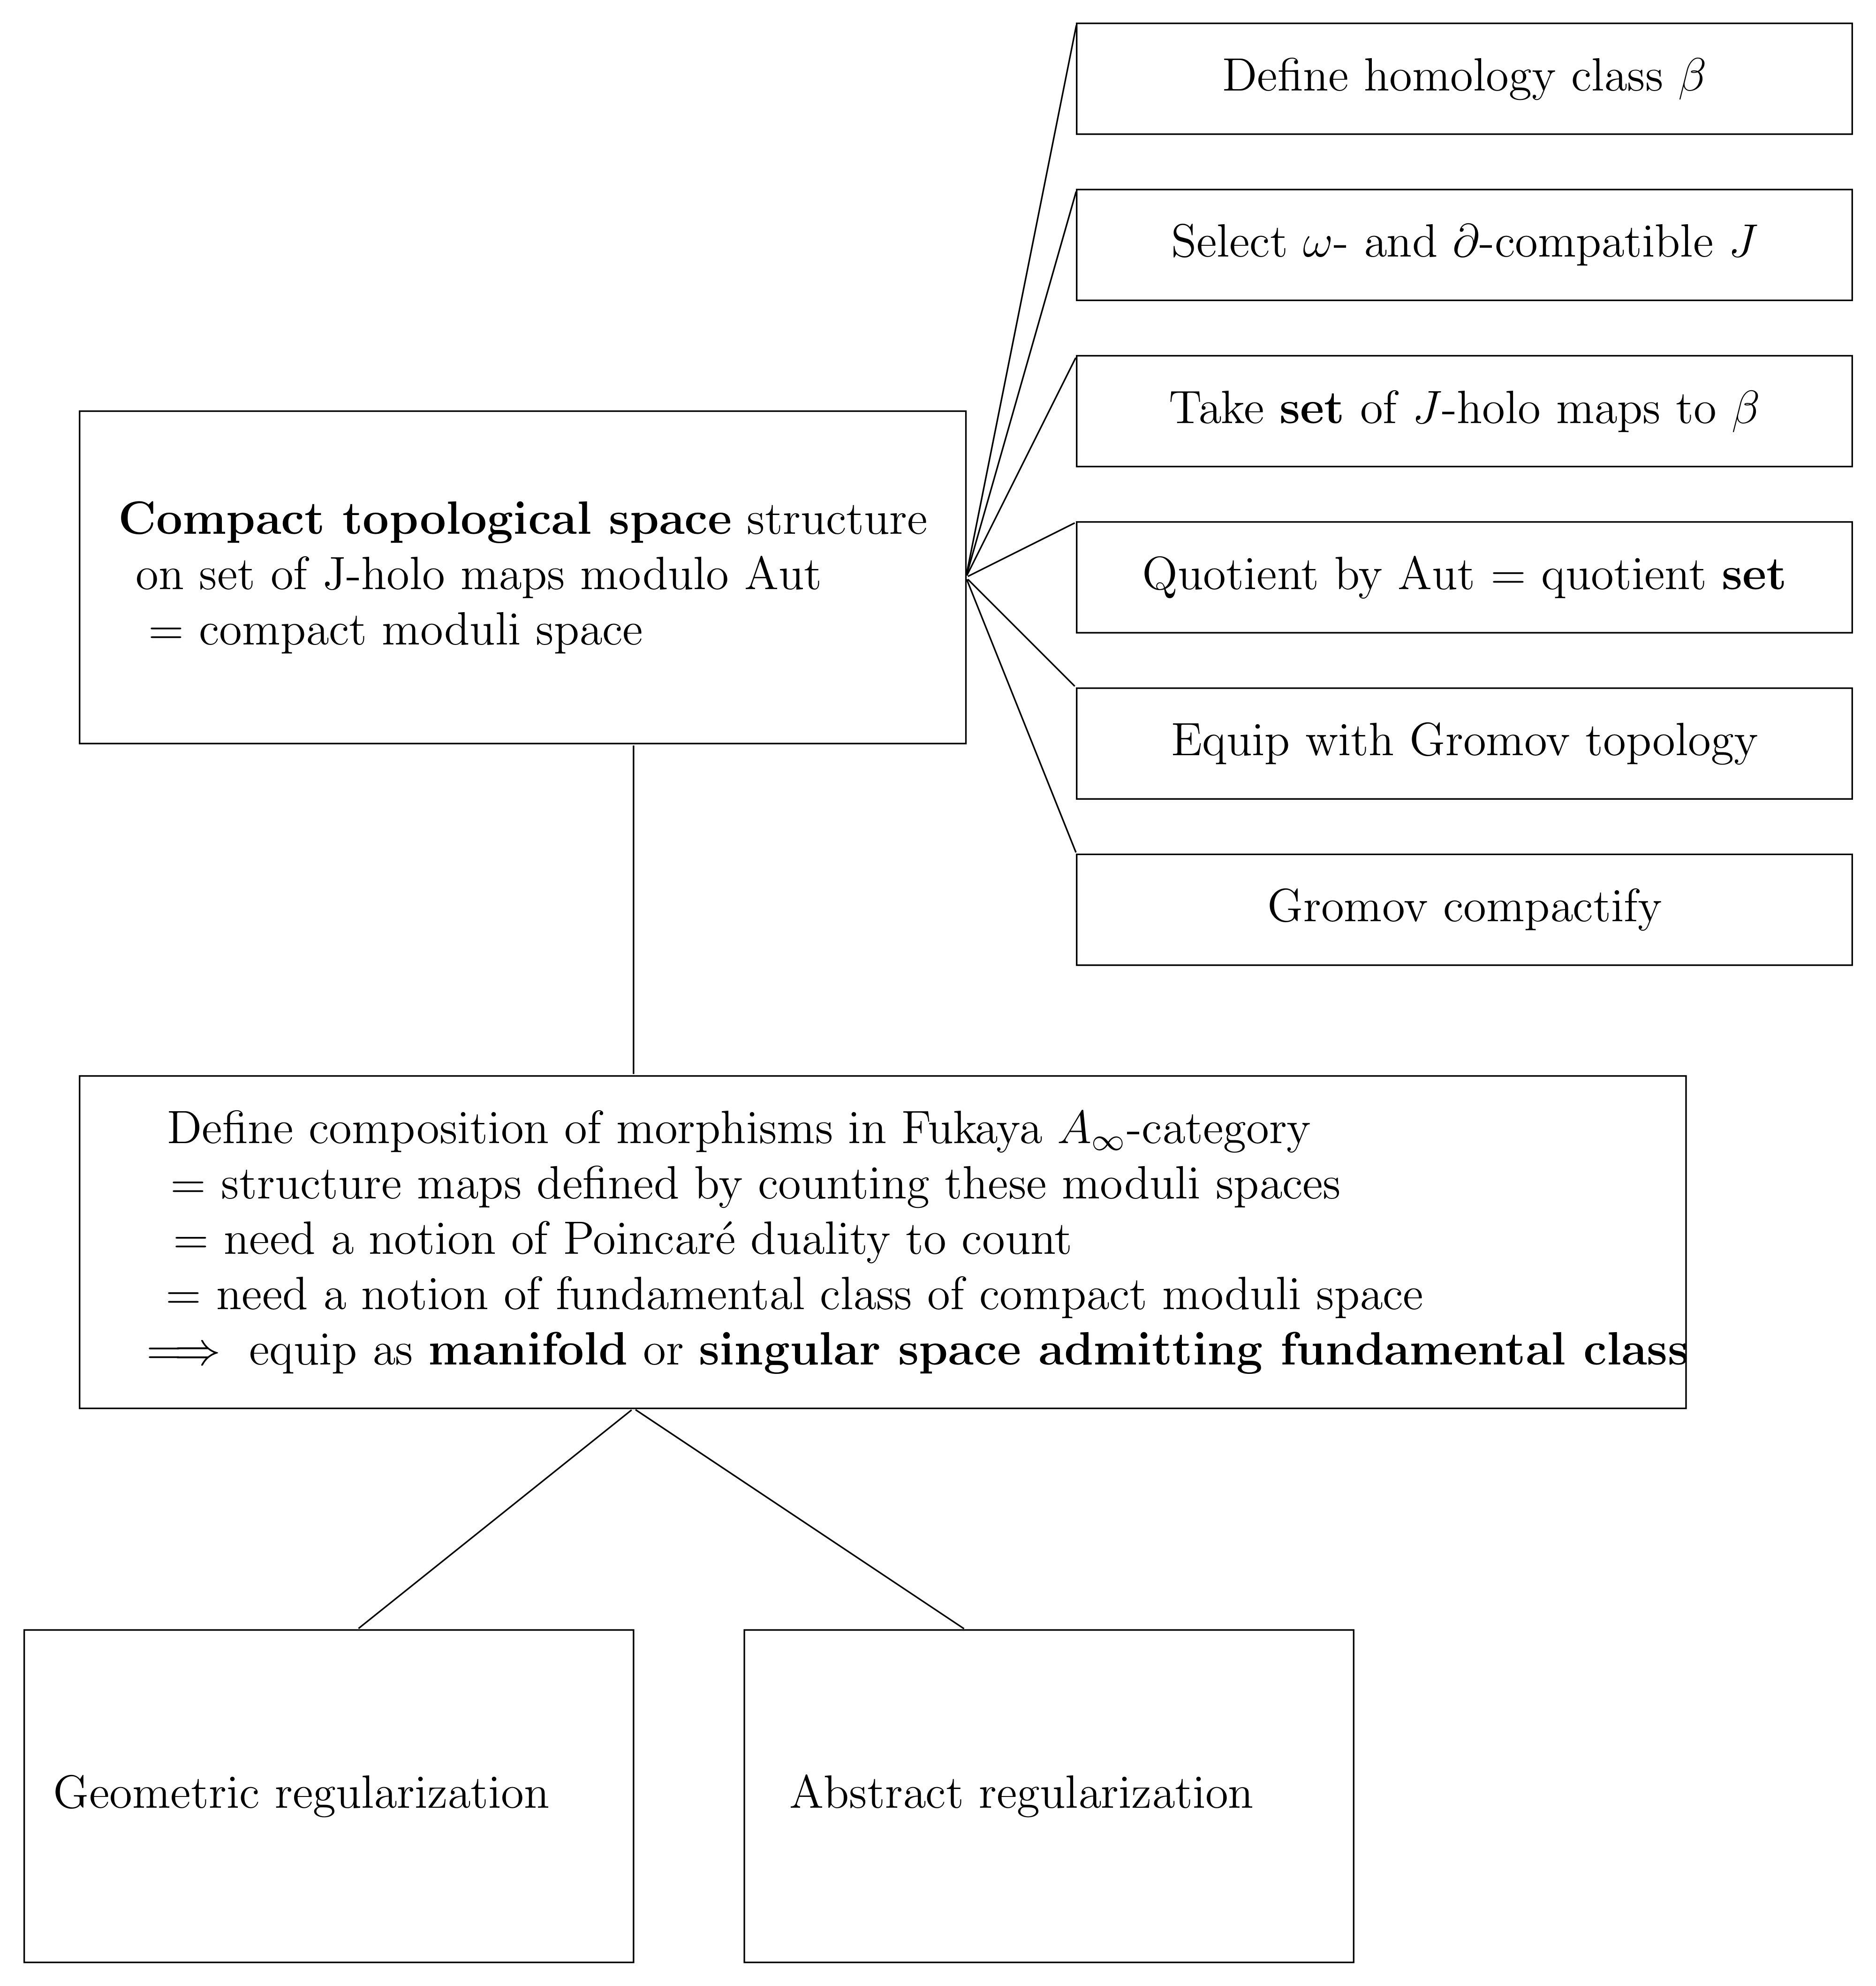
\includegraphics[width=0.84\textwidth]{figures/fig_4_3.png}
\caption{在深谷范畴中处理模空间的流程图（原书 p.96）}
\label{c7:fig-flow}
\end{figure}

% ===== 原书 p.97 =====

\begin{figure}[htbp]
\centering
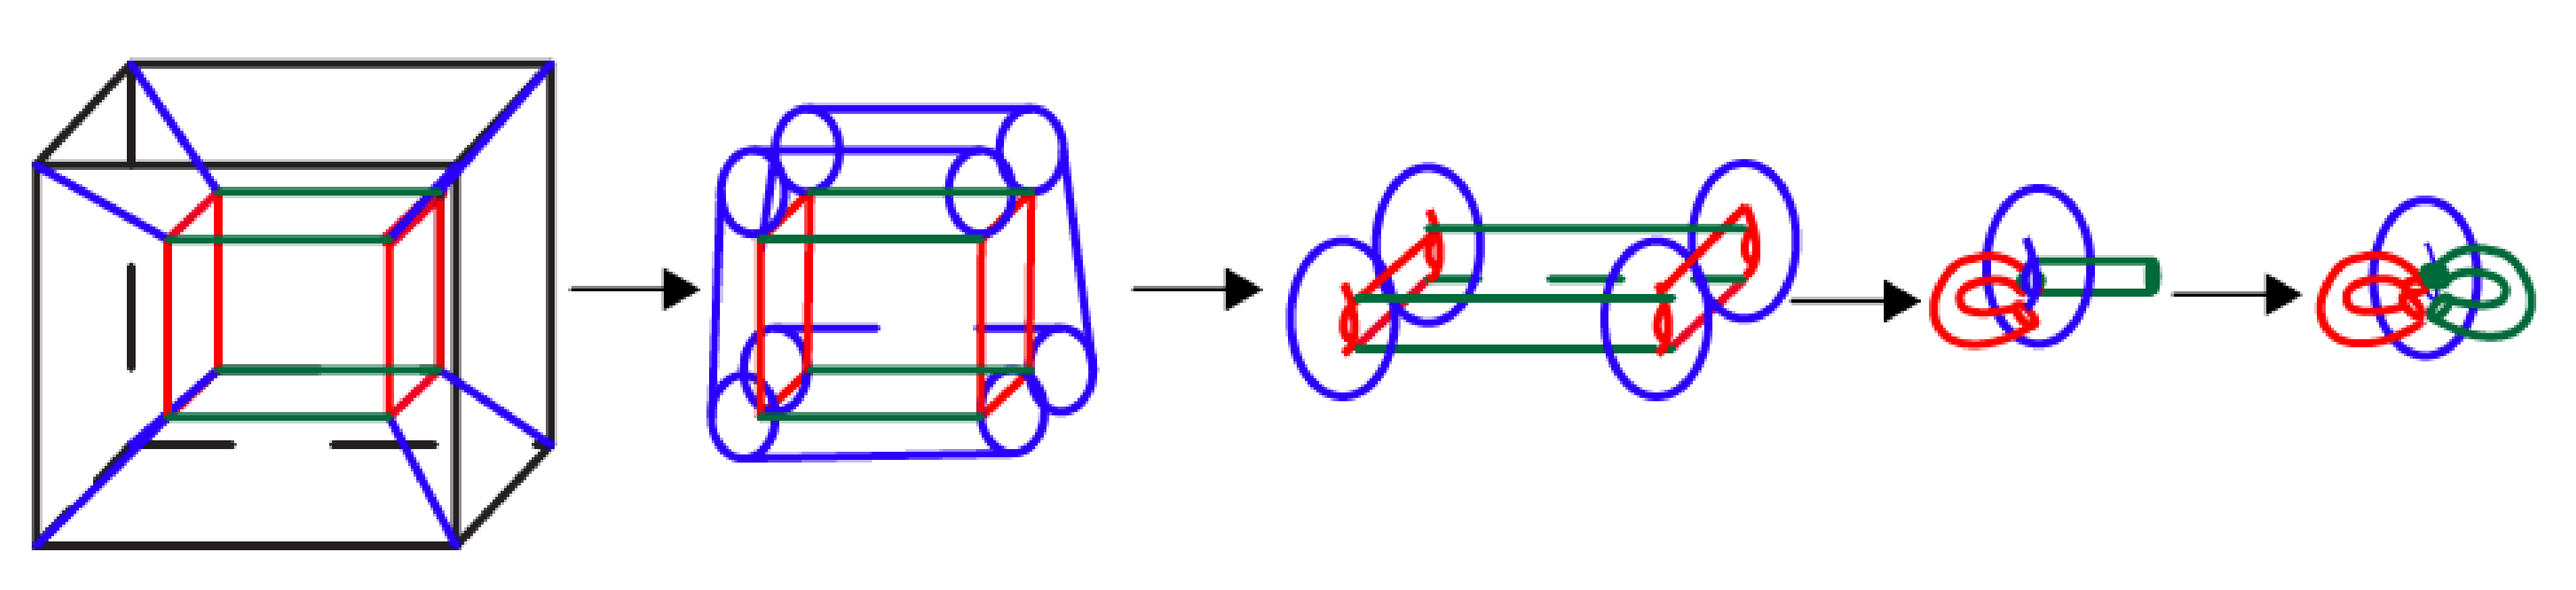
\includegraphics[width=0.95\textwidth]{figures/fig_4_4.png}
\caption{把 $T^4$ 看成 $4$-立方体的商所得胞腔复形的 $2$-骨架（原书 p.97）}
\label{c7:fig-2skeleton}
\end{figure}

\begin{remark}\label{c7:rem-spectral}
注意，我们把拓扑纤维化的谱序列直觉用到了纤维化 $v_0\colon Y\to\C$ 上。
它在代数几何意义下是纤维化，在代数拓扑意义下却不是，因为没有同伦提升性质。
例如取原点附近一个圆盘，由于奇点，把它提升上去有 $S^1$ 个选择。
也就是说，$T^4$ 与它的退化纤维 $\C\PP^2(3)/\Gamma_B$ 并不弱同伦等价。
若情形对得上，谱序列的第二页应是
\[
E^2_{p,q}=H_p(\C,H_q(T^4)).
\]

代数地看，带局部系统数的同调就是 $C_*(\tilde X)\otimes_\pi H_q(F)$。
这里 $\pi=\pi_1(\text{底空间})$ 作用在覆盖空间 $H_q(F_b)\mapsto b$ 上，取离散拓扑。
于是沿底空间中的单值性可以看见 $H_1(F_b)$ 的元素如何变化，这个变化给出 $\pi$ 的作用。
该链复形上的微分是 $\partial\otimes1$。
当万有覆盖 $\tilde X=\text{底空间}=\C$ 可缩时，$\pi_1$ 平凡，张量积就回到通常同调：$p>0$ 次为零，$p=0$ 次给出底空间的同调。
\end{remark}

\transnote{这里在解释「为什么不能直接用 Leray 谱序列算 $H_2(Y)$」：$v_0$ 只有代数几何的纤维化结构，没有同伦提升，故 $H_*(Y)$ 不能由 $H_*(\C,H_*(T^4))$ 的谱序列读出。作者的替代办法是先算中心纤维，再用 Mayer--Vietoris。}

\begin{remark}\label{c7:rem-toric}
另一种算法用 [CLS11] 的环簇理论。环簇 $X$ 内含一个稠密的 $(\C^*)^n$。
它是 $n$ 个柱面，可缩到 $n$ 个圆上，故 $\pi_1=\Z^n$。此外它满射到 $\pi_1(X)$，所以 $\pi_1(X)$ 总是 $\Z^3$ 的商。
本例在取商之前是 $\Z^4$：多面体中心给一个 $\PP^1$，三次爆破再给三个。
取商之后，香蕉流形中的三个 $\C\PP^1$ 加起来等于一个矩映射纤维与一个被捏的 $T^3$；特别地，第四个生成元是前三个之和。

令 $Z:=\widehat{\C\PP^2(3)}/\!\sim$，它的多面体由六边形的无限铺砌给出，正是 $\tilde Y$ 的中心纤维。
它是万有覆盖，理由是由环簇理论 $\pi_1(Z)=0$。
于是 Hurewicz 定理给出 $\pi_2(Z)=H_2(Z)$，进而 $\pi_2(\C\PP^2(3)/\!\sim)=\pi_2(Z)$。
因此要算 $H_2(\C\PP^2(3)/\!\sim)$，也可改用下面的 Mayer--Vietoris。

在六边形图中挖去一个开集，它会收缩到边界上。这样得到两个开集；在矩映射图像里，它们是一个圆盘与其补集，交于一个 $S^1$。

令 $B:=D^2\times T^2$ 对应矩多面体中的圆盘。令 $\tilde A$ 为其补集，是一圈 $6$ 个 $\C\PP^1$；再令 $A:=\tilde A/\Gamma_B$ 为香蕉流形。于是
\end{remark}

% ===== 原书 p.98 =====

\[
\begin{aligned}
0=H_3(\tilde A)\oplus H_3(B)&\longrightarrow H_3(Z)=0\\
&\longrightarrow H_2(\tilde A\cap B)=\Z^3
  \xrightarrow{\ (*)\ } H_2(\tilde A)\oplus H_2(B)=\Z^6\oplus\Z
  \longrightarrow H_2(Z)\longrightarrow 0\\
H_1(\tilde A\cap B)=\Z^3&\xrightarrow{\ \cong\ } H_1(\tilde A)\oplus H_1(B)=\Z\oplus\Z^2
  \longrightarrow H_1(Z)=0
\end{aligned}
\]
其中
\[
(*)=\begin{pmatrix}
1&0&0\\
0&1&0\\
-1&1&0\\
-1&0&0\\
0&-1&0\\
1&-1&0\\
0&0&1
\end{pmatrix},
\]
并且倒数第二个映射关于 $H_2(\tilde A\cap B)=H_2(S^1\times T^2)$ 的三个生成元是 $3\times3$ 恒等矩阵。
这三个生成元如下记：$b$ 记矩多面体中的 $S^1$，$T_1,T_2$ 记 $2$-环面纤维中的两个圈。
% [Tutor Note: 原文「倒数第二个映射」此处指 H_1 行的同构，却又说以 H_2(Ã∩B) 的生成元为基；H_1 与 H_2 的生成元一一对应，读者按后者理解即可。]

再对 $\C\PP^2(3)/\!\sim$ 取商，得到
\[
\begin{aligned}
0=H_3(A)\oplus H_3(B)&\longrightarrow H_3(\C\PP^2(3)/\!\sim)=0\\
&\longrightarrow H_2(A\cap B)=\Z^3
  \xrightarrow{\ (**)\ } H_2(A)\oplus H_2(B)=\Z^3\oplus\Z\\
&\longrightarrow H_2(\C\PP^2(3)/\!\sim)=\Z^4
  \longrightarrow \Z\cdot b\subset H_1(A\cap B)=\Z^3
\end{aligned}
\]
\[
\begin{pmatrix}
0&0&0\\
0&0&0\\
0&1&0\\
0&0&1
\end{pmatrix}
\longrightarrow H_1(A)\oplus H_1(B)=\Z^2\oplus\Z^2
\longrightarrow H_1(\C\PP^2(3)/\!\sim)=0,
\]
其中
\[
(**)=\begin{pmatrix}
0&0&0\\
0&0&0\\
0&0&0\\
0&0&1
\end{pmatrix}.
\]
% [Tutor Note: 原书此处自相矛盾：序列中的 4×3 矩阵第三行为 (0 1 0)，而页面下方「where (**)=」给出的矩阵第三行全零。译文照录两处，未作统一；请读者以序列中实际出现的矩阵为准，此点已登记疑点。]

所以最终我们看的是 $6$ 个 $\PP^1$ 射到三个粘起来的 $\PP^1$ 上的投影。同调仍是 $\Z^4$。

到这儿，我们知道了 $Y$ 中可以出现球泡像的同调类。还需要知道：边界落在给定拉格朗日上的圆盘的相对 $H_2$。
回忆背景一节中对映射与截面的讨论。下面定义本文要用的圆盘。
我们考虑的 $\pi_2(Y,L)$ 中的类覆盖底空间中 $0$ 附近的一个圆盘，并以一个点穿过中心纤维。
变动这个点，借助中心纤维的环簇几何可以枚举所有同调类，见 [CO06]。
这一点留到下文对某个 $J$ 计算圆盘计数时再说。这里只证明：给定 $H_2(Y,L)$ 中的同调类 $\beta$，相应模空间存在。

% ===== 原书 p.99 =====

\begin{definition}[类截面映射]\label{c7:def-section-like}
取原点附近的一个开集，记为 $U$。只考虑在 $U$ 外恒等于 $J_0$ 的近复结构。于是在 $U$ 外，圆盘就是截面。
由 Riemann 映射定理：若处处取 $J_0$，把该处的 $J_0$-全纯映射经也全纯的 $v_0$ 复合到底空间，这样的映射唯一。

为了得到足够好的正则性，需要允许 $J$ 在 $U$ 内部偏离 $J_0$。
具体地，下文所有拉格朗日都要求经过底空间中的点 $-1$。于是取 $U$ 为半径小于 $1$ 的圆盘，就可断定没有多重覆盖的圆盘，因为这类圆盘绕不过边界。
就取 $U$ 为以原点为心、半径 $1/2$ 的圆盘。

还能排除盘起泡与条带断裂：纤维中没有圆盘，因为环面中的线性拉格朗日相对 $\pi_2$ 为零，即它们不围出圆盘。
也不会有绕原点附近开集上圆盘边界的盘，因为它在 $-1$ 附近必须是一一的。
因此另一个盘或条带只能落在底空间圆周的真子集上方，而纤维化在那里可平凡化。
假设圆盘的边界落在 $U$ 外（但此时还需证明它对 Hamilton 同痕不变）；或者把盘在 $-1$ 附近的 $1$-$1$ 性质延拓到盘边界的其余部分。
两种做法都给出：由 $1$-$1$ 性质，这种盘的边界缩成一点；而环面中没有球，故该盘必为常值（或再次使用 $1$-$1$ 性质）。

若真出现多重覆盖，可以要求 $J$ 依赖 $z\in S$，即把 $J$ 换成 $J_z$。
[MS12] 为拉格朗日边界情形奠定了这一基础，[Aur14] 有具体描述，其中涉及条带上的一族 $\R$-参数 $J$。不过我们这里用不上。
\end{definition}

\transnote{取「半径 $<1$、圆心在原点」的 $U$，配合「拉格朗日过 $-1$」这条要求，是为了让任一多重覆盖盘都绕不到 $U$ 的边界上，从而被排除。若把 $U$ 取大，这条论证就断了。后文所有 $L_i$ 都过底空间中的 $-1$，原因也在此。}

\begin{corollary}\label{c7:cor-J-curve}
$J$-全纯曲线有一些与复曲线类似的性质。例如 Carleman 相似原理：一条近似满足 CR 方程的曲线，可经后复合一个映射，改为满足以 $J_0$ 写出的 CR 方程。这是辛流形 $\R^{2n}$ 的情形。
其余推论包括：唯一延拓，即两个 $J$-全纯映射若在开集上相等，或在一点处所有导数相等，则两者相等；原像中只有有限个点，临界点也只有有限个；简单曲线的单射点集是开稠密的。
\end{corollary}

曲线的像落在 $Y$ 的哪些同调类，前面已经讨论完。接下来证明正则 $J$ 存在。
有了它，就能构造一个 Fredholm 问题：Cauchy--Riemann 算子 $\bar\partial_J$ 作为 Banach 丛的截面切出模空间，再由隐函数定理得知零点的原像是流形。
这样就能给模空间安上光滑结构。

% ===== 原书 p.100 =====

\begin{example}\label{c7:ex-banach-analogy}
这是无穷维 Banach 空间中的一个类比。先看有限维的例子：$f\colon\R^3\to\R$，$f(x,y,z)=x^2+y^2+z^2$，在 $(x,y,z)\neq0$ 处正则，因为
\[
\de f|_{(x,y,z)}=(2x,2y,2z)^{\mathsf T}
\]
满射。于是 $f$ 是正则函数，$1$ 的原像是光滑流形（球面）。
在 Banach 丛的设定中，「正则」不仅要求满射，还要求右逆存在。
\end{example}

区别在于这里的微分算子以函数为输入，于是进入无穷维 Banach 空间的世界。
下面的理论沿用 [MS12, 第 3--10 章] 的论证，但针对带边曲线；[Sei08] 也有讨论。
[Weh13] 用几何正则化理论处理 Gromov 非挤压定理，示范了如何证明随 $J_t$ 变化的模空间族是 $1$ 维的（Fredholm）、是流形（横截/正则）、是紧的（Gromov 紧性），且有边界。
抽象正则化理论的好参考是 [Weh14]。

下面证明正则 $J$ 存在。

\begin{lemma}[几何正则化]\label{c7:lem-geometric-reg}
存在稠密子集 $\cJ^1_{\mathrm{reg}}\subset\cJ(Y,\omega)$，由在 $U$ 外恒为 $J_0$ 的 $\omega$-相容近复结构 $J$ 组成，使得对一切 $J$-全纯映射
\[
u\colon(D,\partial D)\to(Y,L|_\gamma),
\]
线性化 $\bar\partial$ 算子 $D_u$ 满射。这里的拉格朗日边界条件由「在底空间中从 $-1$ 出发绕 U 形平行移动纤维拉格朗日」给出。
\end{lemma}

\begin{remark}\label{c7:rem-superscr}
上标 $1$ 是为了后文：还要更小一些的 $\cJ^2_{\mathrm{reg}}$ 与 $\cJ^3_{\mathrm{reg}}$，分别对「盘接盘」「盘接球」正则，边界条件类似，标号取 $2$、$3$。
它们不仅要求线性化算子满射，还要求交点处的取值行为相容。
\end{remark}

\begin{proof}[{略证，改写自 [MS12] 第 2 版第 55 页编号 3.1.6(ii) 那条定理的证明}]
我们给一张路线图，把 McDuff--Salamon 的做法改写到带拉格朗日边界条件的情形。
相关背景也取自 [Weh14, 第 9 讲]；细节在 2017 年 9 月 8 日的 Denis 讨论班上讲过。
[MS12] 的定理 C.1.10 证明：带边界情形确有 Fredholm 问题。

\textbf{引言。}「正则化」指扰动 $\bar\partial_J$ 算子，使它等变横截于某个 Fredholm 丛的零截面；该丛可造得让这个算子成为其截面。
「几何正则化」指扰动来自对近复结构 $J$ 的扰动，因而具有几何来源。也就是说，$J'$ 变动时 $\bar\partial_J$ 的扰动是 $\bar\partial_{J'}-\bar\partial_J$。
在这种设定下，等变性自动成立，下文会说明。
注意后文计算要用非正则的 $J$；那时改用「抽象正则化」，即加抽象扰动 $\nu$。
$\nu$ 仍是同一 Fredholm 丛的截面，但不必是 $\bar\partial_{J'}-\bar\partial_J$ 的形式。
\end{proof}

\transnote{「几何正则化」与「抽象正则化」的区别是本节的主线：前者扰动 $J$ 本身，后者在 Fredholm 丛上加抽象截面 $\nu$。前者能做是因为 $J$ 的空间足够大且在边界附近已固定；后者在计算时不得不用，因为圆盘计数只需要 $J$ 的拓扑信息，而不需要它正则。}

% ===== 原书 p.101 =====

为证明「映到沿 U 形曲线平行移动所得纤维拉格朗日」的圆盘存在正则 $J$，我们证明这类 $J$ 在
\[
\cJ^\ell_\omega(Y,U):=\{J\in\Gamma(TY)\mid J^2=-1,\ J|_{Y\setminus U}\equiv J_0,\ J\in C^\ell\}
\]
中稠密。
在 [Sei08] 中它记作 $\cJ^\ell_F$，其中 $F$ 指「平行移动纤维拉格朗日」所得的拉格朗日边界条件，他称之为运动边界条件（moving boundary condition）。
带边界情形需要的正是这个 $J$ 集，参看 [MS12, Remark 3.2.3]。

先定义由变 $J$ 编码的「全体 $W^{k,p}$ 映射 $u$ 与几何扰动」之集：
\[
\cM_J:=\{(u,J)\mid J\in\cJ^\ell_\omega(Y,U),\ W^{k,p}\ni u\colon(D,\partial D)\to(Y,L)\}.
\]

$k$ 充分大时 $W^{k,p}\subset C^\ell$。再由椭圆自举可知 $J$-全纯映射 $u$ 属于 $C^\ell$。
这个模空间称为「万有的」，因为允许 $J$ 变动。
用 $W^{k,p}$ 是因为它完备，即 Banach 空间；在函数空间的无穷维设定里调用 Sard--Smale 与椭圆正则正需要这一点。
特别地，我们希望 $\cM_J$ 是 $C^{\ell-1}$ 的可分 Banach 流形。
然后对投影 $(u,J)\mapsto J$ 用 Sard--Smale，就得到圆盘的正则 $J$ 构成稠密集。

\textbf{Banach 丛的搭建。}
我们要把 $\cM_J\subset\cB^{k,p}\times\cJ^\ell_\omega(Y,U)\ni(u,J)\mapsto J$ 看成某个 Banach 丛的 Fredholm 截面，以便用 Sard--Smale 得到稠密的正则值集。
Fredholm 是满射的推广。在无穷维设定中还要求右逆存在；最近那篇 polyfold 文章里就有右逆不存在、且仅此不够的例子。
随后隐函数定理给出：该截面的零点切出的 $(u,J)$ 之集是底空间的 Banach 子流形，而不只是子集。
注意零点集正是使 $u$ 为 $J$-全纯的那些 $(u,J)$。

$\cB^{k,p}\ni u$ 上的 Banach 流形结构：在任意映射 $u$ 附近构造局部 Banach 图。
局部模型是 $T\Gamma(u^*TY,u^*TL)\ni\xi$，映射为 $u\mapsto\exp_u\xi$。
这是良定义的：总存在度量使一个拉格朗日全测地 [MS12, Lemma 4.3.4]；也就是说，从某个度量看，一个拉格朗日（或两个）是全测地的。
所考虑的点处至多有两个拉格朗日相交，所以够用。
带拉格朗日边界条件时，正需要全测地性来保证这给出图：给定 $\partial D$ 上一点，沿该点处放置的向量 $\xi$ 走，结果仍切于 $L$，于是测地线留在 $L$ 中。

$\cJ^\ell_\omega(Y,U)\ni J$ 上的 Banach 流形结构（它是所造 Banach 丛底空间的第二个因子，参看 [MS12, §3.2]）：同样用指数映射得到 $\dot J$。
$J$ 的三个条件线性化：1）$J|_{Y\setminus U}\equiv J_0$ 给出 $\dot J|_{Y\setminus U}\equiv0$，这是拉格朗日边界情形特有的；2）$J^2=-1$ 给出 $\dot JJ+J\dot J=0$；3）$\omega(\cdot,J\cdot)>0$ 且对称这一条也线性化。
图由 $J\mapsto J\exp(-\dot JJ)$ 构造。参看 [Sei08]。
丛的纤维不带边界条件，因为它由 $(du)^{0,1}=\frac12(du+J\circ du\circ j)$ 的落点空间给出，与边界无关。
至于切于边界的方向会发生什么，则不得而知，因为 $J$ 与 $j$ 可能把它们拧来拧去。

% ===== 原书 p.102 =====

下面说明如何在底空间的开集上搭起 Banach 丛的结构。这部分照抄 [MS12] 的做法，因为纤维上没有边界条件。
在 $\cB^{k,p}\times\cJ^\ell_\omega(Y,U)$ 的第一个因子上，用指数映射在邻域 $\cN(u)$ 上平凡化丛；在第二个因子上，用平行移动在邻域 $\cN(J)$ 上平凡化。
两者合起来把丛在底空间的一个邻域上平凡化；这些平凡化复合得到的过渡映射满足 Banach 丛的条件，见 [MS12] 与 [Sei08]。

\textbf{Fredholm 问题。}
Fredholm 问题就是 Banach 丛的 Fredholm 截面。
所谓 Fredholm 截面，指线性化为 Fredholm 算子的截面：$\dim\Ker-\dim\Coker$ 有限（例如到纤维切空间的投影满射），且像闭。
更一般地，它把模空间（主体部分，以及作为纤维积出现的 Gromov 紧化成分）搭成若干 Fredholm 截面的零点集。

我们断言截面 $(u,J)\mapsto\bar\partial_J(u)$ 是 Fredholm 的。
要取 $\bar\partial$ 算子在映射 $u$ 处的线性化，须看 $u$ 沿切向量 $\xi$ 作无穷小变动时会发生什么。
也就是把 $\bar\partial$ 算子放在一族中求导，再取零处的导数，见 [MS12, Proposition 3.1.1]。
同理，$J$ 沿切向量 $\dot J$ 作无穷小变动。
\[
\cF_u\colon W^{k,p}(S,u^*TY)\to W^{k-1,p}(S,\Lambda^{1,0}\otimes_j u^*TY).
\]

$D_u$ 的定义如下：对 $u$ 的指数邻域中附近的 $u'$，取 $D_{u'}\bar\partial_J$，把它沿平行移动送回 $u$ 处图的原点，作用 $\bar\partial_J$，再沿平行移动推回纤维上。
线性化算子 $D_u\xi$ 就是这一操作在 $0$ 处的导数。由上面全测地的条件，这是良定义的。
以上只变 $u$。若同时变 $J$，得到 [Weh14, 第 9 讲]：
\[
D_u\xi+\frac12\dot J\,\de u\,j .
\]

特别地，它满射且有右逆，从而是 Fredholm 的。理由如下。
反设像不稠密，取像的正交补中一个非零线性泛函 $\eta$。
令 $\dot J=0$，可见 $\eta$ 也正交于 $\mathrm{im}(D_u)$。于是它对一切 $\dot J$ 都正交于 $\dot J\,\de u\,j$。
但用鼓包函数，由 $\eta\neq0$ 可构造扰动 $\dot J$，使 $\eta$ 作用在其上的积分非零，矛盾。见 [MS12, 第 65 页]。

在拉格朗日边界情形中这个构造仍可行：所构造的 $\dot J$ 支在某个「某处单射」点附近的小邻域内，因此在边界附近为零，正合要求。
某处单射点稠密，故可在 $\eta$ 非零的给定点附近找到一个；特别地，这类点有邻域。
用鼓包函数构造 $\dot J$，使 $\int_D\eta(\dot J\,\de u\,j)>0$。这推出矛盾。

% ===== 原书 p.103 =====

于是 $\eta$ 在单射点的开集上为零，由唯一延拓 [MS12, Theorem 2.3.2] 恒为零。
这又与 $\eta\neq0$ 矛盾。故原假设「像不稠密」不成立。
像稠密；又因它闭，故满射且有右逆。

\textbf{Sard--Smale 与反函数定理。}
有了 Fredholm 问题，就可以用 [MS12, 附录 A：Fredholm 理论] 中关于 Banach 空间的结果。
特别地，我们满足 [MS12, Theorem A.5.1（Sard--Smale 定理）] 的假设，而该定理依赖无穷维反函数定理 [MS12, Theorem A.3.1（反函数定理）]。
Sard--Smale 的结论是：正则 $J$ 之集在全体 $J$ 中稠密，正是我们的目标。于是正则 $J$ 存在。

\begin{remark}[记号]\label{c7:rem-notation-Jdot}
注意：记号 $\dot J$ 并不意味着只能在某个方向上变 $J$，通常点记号有此含义。
这里只是把 $\dot J$ 当作「复结构空间切向量」的象征性写法。
文献中这个空间常记作 $Y$，但本文 $Y$ 指 A 侧的流形。
\end{remark}

\begin{lemma}\label{c7:lem-param-discs}
对 $J\in\cJ^1_{\mathrm{reg}}(Y,\partial Y)$，参数化的 $J$-全纯圆盘 $u\colon(D,\partial D)\to(Y,L|_\gamma)$ 之集是有限维流形。
\end{lemma}

\begin{proof}[{取自 [MS12, Theorem 3.1.6(i)] 的证明}]
图由
\[
\cF_u\colon W^{k,p}(S,u^*TY)\to W^{k-1,p}(S,\Lambda^{1,0}\otimes_j u^*TY),
\qquad
\xi\mapsto\exp_u\xi
\]
给出：把 $\cF_u^{-1}(0)$ 中 $u$ 附近的开集微分同胚到 Banach 空间中 $0$ 附近的相应开集。
$J$ 的正则性给出 $\de\cF_u(0)=D_u$ 满射。
隐函数定理 [MS12, Theorem A.3.3] 说明，适当缩小开集后这些就是光滑流形的图。
这与 $k,l$ 无关，因为由椭圆正则 [MS12, Proposition 3.1.10]，$J$-全纯映射 $u$ 是光滑的。
注意 [MS12, 附录 B（椭圆正则）] 已就全实边界条件（例如这里的拉格朗日边界条件）备好所需背景。
此处不重写证明，只定义该节用到的术语，另见 [Weh13, 第 4--6 讲]。
\end{proof}

\begin{itemize}[leftmargin=1.6em,itemsep=0.2em]
\item $C^k_0$：$k$ 次连续可微，且到该阶为止的导数在无穷远处趋于零。
\item 检验函数的 Schwartz 空间 $\zeta$：满足 $f\cdot(\sqrt{1+|x|^2})^k\in C_0$ 的 $f$。
      它对卷积封闭，且结合。缓增分布（tempered distributions）$\zeta'$ 指其对偶空间。
      特别地，$\zeta\hookrightarrow\zeta'$，嵌入由连续稠密单射 $f\mapsto\int_{\R^n}f\cdot(\cdot)\,\de^nx$ 给出。
\item 说一个等式「弱意义下成立」，意思是「对所有缓增分布积分后成立」。
\end{itemize}

% ===== 原书 p.104 =====

\begin{itemize}[leftmargin=1.6em,itemsep=0.2em]
\item Fourier 变换在 Schwartz 空间上是连续映射，并把卷积变成乘法。
\item Sobolev 空间 $W^{s,2}$：满足 $F.T.(f)\cdot(\sqrt{1+|x|^2})^k\in L^2$ 的 $\hat f\in\zeta'$。
      $W^{k,p}$：到 $k$ 阶的导数弱意义下属于 $L^p$。
      特别地，$k\gg l$ 时有紧支的 Sobolev 嵌入 $W^{k,p}\subset C^l$。
\item 函数 $u$ 的支集是「$u=0$ 处」在弱意义下的补集。
      分布 $u$ 的奇支集，指弱意义下挖掉那些具有局部紧光滑性的 $u\in\zeta$ 之后剩下的部分。
% [Tutor Note: 原文这句「The singular support of a distribution means we remove, in a weak sense, u ∈ ζ with no local compact smoothness」表述含混，字面如此照译，请读者按标准定义（奇支集 = 光滑性失效处的闭集）理解。]
\item 椭圆正则：$p(D)u$ 光滑，当且仅当 $p(D)$ 的奇支集为空，当且仅当 $u$ 光滑。
      特别地，$\bar\partial u=0$ 推出 $u$ 光滑。
      当 $p>2$ 时，导数的 $L^p$ 界给出紧模空间。
      $p=2$（即 $L^2$ 范数）时这一点失效，于是可能起泡，泡不在模空间里。
      要紧化，就商掉区域的自同构群，并确定可能起什么泡。
      随后需要把泡现象粘回主体，才能得到紧流形。这些 Gromov 紧性现象见 [Weh13, 第 7--9 讲]。
\end{itemize}

\begin{remark}\label{c7:rem-nonregular-J}
即使 $J$ 非正则，仍可用上面的办法，借助 [MS12, Theorem C.1.10（Riemann--Roch）] 构造 Fredholm 问题；该定理已在拉格朗日边界情形下证明。
但光滑结构从何而来是另一回事，因为 $J$ 不正则。抽象扰动可能正是在这里派上用场。
\end{remark}

\begin{example}[区域的模空间]\label{c7:ex-dm-space}
Deligne--Mumford 空间：把稳定曲线（亏格 $g$、$k$ 个标记点）映到一点，再对重参数化取商。
要紧化并纳入所有可能的余维 $1$ 构型，即稳定曲线的极限，需考虑合适的对偶图。参看 [Sei08, §9] 与 Liu 关于对偶图的文献。

一棵树记录如何粘接：内部边配一个粘接长度，两端半无限边给出最终粘好的圆盘的标记点。
想法是：我们有一族圆盘，由底空间中可能的循环构型参数化；每条内部边还配一个粘接参数。
内部边越多，底空间维数越高，因为泡占掉的余维越多。

再把所有 $d$ 叶树添进去，就得到该族底空间的紧化。
只要 $\overline\cR^{d+1}$ 上第二可数与 Hausdorff 两条成立，就能定义连续性、拓扑与光滑性。
按 FOOO 的说法，这些性质是从 Deligne--Mumford 空间 $\overline{\cM}_{0,d+1}$ 的实轨迹子集继承来的，因为粘接参数是实的。
多边形正则性与层论解释另见 [Sei08, §13]。
\end{example}

% ===== 原书 p.105 =====

\begin{claim}\label{c7:claim-expected-dim}
给定 Fredholm 截面，可以算出参数化曲线流形的预期维数；未参数化曲线的模空间维数比它少三。此外还有诱导定向。
\end{claim}

Morse 理论中的类比：有了 Morse--Smale 数据，数特征值就知道模空间的维数。
$x^-$ 的不稳定流形与 $x^+$ 的稳定流形横截相交；投影映射从不稳定流形打到稳定流形的正交补。
Fredholm 截面的指标是 Hessian 的谱流（Morse 情形则是数 Hessian 矩阵的特征值）。
谱流来自 $(J_0\partial_t+S_s)_{s\in\R}$；$D_u$ 等于它加上 $\partial_s$ 再加一个紧扰动。

\begin{claim}\label{c7:claim-aut-action}
$\Aut$ 光滑地作用在参数化曲线流形上，故模空间 $\widehat\cM/\Aut$ 是光滑流形。
\end{claim}

\begin{claim}\label{c7:claim-gluing}
用粘接可以给紧化后的模空间安上光滑结构。所粘接的构型正是 Gromov 紧性中出现的那些。
于是得到光滑紧 $0$ 维流形的结构，可以数了。
\end{claim}

\begin{proof}[{略证，参看 [MS12] 与 [Weh13]}]
Gromov 紧性由若干结果推出，例如等周不等式
\[
|a(\gamma)|\le C|\mathrm{length}(\gamma)|^2,
\]
可去奇点定理与能量衰减。
这些结果告诉我们圆盘可能的极限构型有哪些：边界点处的盘泡、球泡，或条带断裂。
\end{proof}

\textbf{作为拓扑空间紧化。}
然后说明任一盘泡、球泡或条带断裂都是某列 $J$-全纯曲线的极限。
做法是先预粘接：把这些映射拼起来，拼出的可能不是 $J$-全纯的；再用 Newton 迭代把它变成 $J$-全纯映射。

结论是：未参数化模空间的边界，即 $\widehat\cM/\Aut\setminus\cM/\Aut$，是若干模空间在交点处取纤维积的结果。
例如会出现一个成分，由盘的模空间与球的模空间在公共交点上取纤维积，用以计入球起泡。
% [Tutor Note: 原文文字层两处均写作带帽的 M/Aut；页图上第一项的 M 除 hat 外还多一条上划线，第二项只有 hat，原书此处上划线疑为排版残留。译文第一项取 \widehat\cM、第二项取 \cM（据上下文应为未紧化部分，此时两项不同，差集非空）。]

\textbf{作为光滑流形紧化：极限构型的正则 $J$ 存在。}
要完成「模空间是紧光滑 $0$ 维流形」的略证，还需为这些额外的纤维积构型证明正则 $J$ 存在。
如上所述，靠 $Y$ 的几何可以排除盘起泡与条带断裂，于是只需考虑中心纤维中的球起泡。
盘与球相接处多出一个点，意味着需要「额外数据」的概念来记账这些特殊点。

\begin{definition}[稳定映射的模空间]\label{c7:def-stable-maps}
稳定映射由一棵树给出，树的每个顶点 $\alpha$ 是一个球泡，只有原本的主球例外。
「稳定」指的是没有非平凡自同构；特别地，固定三个点后就没有非平凡自同构。
伪闭链（pseudocycle）指模空间边界的像在全空间中余维至少为 $2$。
虚拟维数等于 Maslov 指标减去稳定树的边数的两倍。也就是说，每多一个起泡的球，维数降 $2$。
半正（semipositive）指对一般的 $J$，不存在负 Chern 数的 $J$-全纯球；本文正是这种情形，因为是 Calabi--Yau。
所得模空间的定义是：取一族映射，对重参数化取商，再紧化。
\end{definition}

% ===== 原书 p.106 =====

\begin{lemma}[有界能量曲线收敛到树的 Bolzano--Weierstrass 类比]\label{c7:lem-bolzano}
稳定映射的模空间具有 Gromov 收敛性。
\end{lemma}

参看 [MS12, 第 5 章]。记 u.c.s.\ 为「在紧子集上一致收敛」。
若固定同调类中各曲线的导数在某个 $p>2$ 的 $W^{1,p}$ 中有界，则得到 Bolzano--Weierstrass 型结论：任何序列都有收敛子列。
但在临界情形 $p=2$（本文即是），极限可能不在原来的曲线类中。
Gromov 收敛到稳定映射的意思是：对树的每个顶点 $\alpha$，有一族重参数化 $\phi^\nu_\alpha$；标记点保持不动，至少在极限中不动。

我们用下面的术语引入「纳入曲线极限」所需的物件，也就是得到紧模空间。
有限能量仍可能起泡，因为能量在缩放不变：自变量反比缩放，微分形式则按比例缩放。
不过导数可以爆破，例如 $\C\PP^1\to\C\PP^2$，$[x:y]\mapsto[x^2:\eps y^2:xy]$。
它参数化的是 $\C\PP^2$ 中由 $ab=\eps c^2$ 给出的全纯曲线。
$\eps\to0$ 时只得到曲线 $[x:0:y]$。但像的极限其实是两个球 $ab=0$，而不只是 $b=0$，因为 $\C\PP^2$ 中做了重整化：看 $ab=\eps c^2$，令 $\eps\to0$ 得 $ab=0$。

去掉起泡点后，曲线列 u.c.s.\ 收敛到主成分。
要找其余泡成分，取由 $z/R_n$（$R_n\to\infty$）定义的新曲线，并添上一列趋于泡点的点。
主体与各泡的能量之和应等于原能量；极限中能量不变。

$e_i$ 记 $\frac12|\de u_i|^2$。为得到到主成分的 $C^\infty_{\mathrm{loc}}$ 收敛，我们在能量上用 Bolzano--Weierstrass 定理。
主成分在 $S$ 上完全有定义（尽管我们挖掉了泡点），理由是伪全纯映射的可去奇点性质。

\begin{lemma}[稳定映射的 Gromov 紧性，参看 [MS12, Equation (5.1.5)]]\label{c7:lem-gromov-compact}
未参数化曲线（即等价类）模空间的紧化，是「各种可能的泡树对应的未参数化曲线」之并。
\end{lemma}

% ===== 原书 p.107 =====

\begin{proof}[{略证}]
理由是这些就是可能的极限构型。式 (5.1.5) 在特殊点情形给该集合配上拓扑，随后讨论粘接与该设定下的 Fredholm 问题。
\end{proof}

特别地，我们需要粘接，并讨论「一个盘加一个球」的 Fredholm 问题。
然后证明：某处单射的盘与简单球之并的模空间是负维数的流形，即空集，可以排除。

\begin{lemma}[排除本文设定中的起泡]\label{c7:lem-excluding-bubbling}
存在稠密子集 $\cJ^2_{\mathrm{reg}}(Y,\partial Y;D\cup\PP^1)$，其中的 $J$ 对「中心纤维中的简单球与某处单射的盘之并」的模空间正则；该盘是类截面的，故必为简单盘。
\end{lemma}

\begin{corollary}\label{c7:cor-no-bubbling}
上述正则 $J$ 对应的模空间维数为负，即空集。
特别地，任何经过开集 $U$ 的某处单射盘与任意「多重覆盖球与简单球」构型之并，其模空间都可排除。
\end{corollary}

\begin{proof}
Riemann--Roch 定理 [MS12, 附录] 给出：该正则 $J$ 切出的流形维数为负，具体是 $-2$。
Lazzarini 的结果 [Laz11] 说明任何盘都可分解为简单盘；他的另一篇 [Laz00] 证明任何 $J$-全纯盘都含一个简单 $J$-全纯盘。
于是若推论所述构型非空，则「简单盘与简单球之并」给出非常值映射——做法是经多重覆盖分解，取一个穿过该球的简单盘。
这与维数为负矛盾，故这样的非空模空间本就不存在。
\end{proof}

\begin{proof}[{引理 \ref{c7:lem-excluding-bubbling} 的证明}]
对每个成分（盘与球）分别有稠密的正则 $J$ 之集：盘的情形前面已述，球的情形见 [MS12, 第 3 章]。
要证的是：这两个稠密集之交中仍有稠密子集，且在 $0$ 上方盘球相交处行为良好。

\textbf{分别对球与盘的正则 $J$ 稠密集取交。}
考虑
\[
\cU\subset\cJ^2_{\mathrm{reg}}(Y,\partial Y;D\cup\PP^1)\times\cJ^1_{\mathrm{reg}}(Y,\partial Y),
\]
并要求 $u_D(D)\nsubseteq u_{\PP^1}(\PP^1)$；只有球的情形要求像不相等，与此相对。
我们有点态约束：球与盘在一点相接。因此需要赋值映射 $\cU\to Y\times Y$ 的横截性。

用 Sard--Smale 可以推出 $\cU$ 是流形；另需一项检查，涉及各成分上的零化子，如下。这取自 [MS12, 第 6 章]。
设 $L^q$ 形式 $\eta$ 在「盘球交点处取零」的 $W^{1,p}$ 测试向量 $\xi$ 上零化 $D_u\xi$。
无论把该交点看成球上的点（McDuff--Salamon 的做法）还是盘上的点（与 [MS12] 同一证明，只是几何约束更多、空间更小，需要测试的更少），$\eta$ 实际都有 $W^{k,p}$ 正则性。
回忆 [MS12] 的椭圆自举结论是对拉格朗日边界条件证明的。分部积分给出 $D^*\eta=0$。

% ===== 原书 p.108 =====

这是把 Stokes 定理与乘积法则用到 $\ip{\eta}{\xi}$ 上：$\eta$ 与 $\xi$ 在 $1$-形式上作赋值、在丛上作内积。
特别地，$\eta$ 与测试向量 $\xi$ 在边界处都切于拉格朗日，这保证相应的积分为零。

隐函数定理给叉积
\[
\cJ^2_{\mathrm{reg}}(Y,\partial Y;D\cup\PP^1)\times\cJ^1_{\mathrm{reg}}(Y,\partial Y)
\]
安上 Banach 子流形结构；此时再用赋值映射保证横截。
于是对角线的原像不只是子集，而是子流形，正是引理所要的稠密正则 $J$ 之集。
这些在 [MS12, §3.4] 的一系列引理中完成；由于附录中的定理都是对拉格朗日边界条件证的，这些引理适用。

\begin{itemize}[leftmargin=1.6em,itemsep=0.2em]
\item 要赋值映射横截。盘与球须在定义域中的 $0$ 处相交，因为 $v_0$ 的中心纤维正是 $H_2$ 非零之处。
      另外固定盘边界上一点，以消去非平凡自同构。
\item 要证赋值映射横截，只需构造支在小球中的 $\dot J$，每个成分一个球；每个球不与该成分之外的部分相交。
      因为前面看的是各成分模空间乘积中的 $\cU$（那个「半程步骤」），这样的开集找得到。
\item 这可行，因为：1）拉格朗日边界条件给出 $\dot J$ 在边界附近为零，故只支在内部小球上就是这种形式；2）各 $\dot J$ 零延拓后可以相加。
      要检查横截性，需线性化映射满射。于是在余空间 $(0_D,0_{\PP^1})$ 处取两个切向量，再在交点附近的两个小球上构造两个 $\dot J$，即得横截。
\item 要证这样的 $\dot J$ 存在，需要关于「在 $D_u$ 上为零的形式 $\eta$」的正则性与消失性结果。
      因为有了它，$D_u\xi+\frac12\dot J\,\de u\,j$ 就满射到 $W^{k-1,p}$ 空间，我们有足够自由度找到上面的向量。
      带边界条件时，附录中的引理与分部积分都成立：取伴随后边界项是 $\de\ip{\eta}{J\xi}_\omega$；边界上拉格朗日与 $\omega$-相容性一起使该项为零。故这一切在此设定下都行得通。
\end{itemize}

在万有空间中满足点态约束的子集上用 Sard--Smale，得到稠密的正则 $J$ 之集，使盘与球在其交点处的赋值映射横截。
引理 \ref{c7:lem-excluding-bubbling} 证毕。
\end{proof}

\textbf{极限构型构成光滑流形。}
极限构型的正则 $J$ 已有，下面证明 $\bar\partial_J$ 横截地切出
\[
\widehat\cM_D/\Aut\times_0\widehat\cM_{\PP^1}/\Aut,
\]
从而是流形。要得到流形结构，仍需 Banach 丛的一个 Fredholm 截面，且其线性化算子满射、有右逆。

% ===== 原书 p.109 =====

令 $\Sigma$ 为「圆盘在一个固定边界点处与球在原点相接」所得的黎曼面。
如上，给 $W^{k,p}(\Sigma,Y)$ 安 Banach 流形结构：用以切空间为模型的图；切空间是 Banach 流形。
也就是说，用指数映射描述「接近」给定映射 $u$ 的映射：给一点 $u$ 及该点处切方向 $\xi$，沿 $\xi$ 方向的测地线（即所需作用量最小的路径）走时间 $1$，得到新的 $W^{k,p}$ 映射 $\exp_u\xi$，它把 $u$ 处处沿 $\xi$ 方向略微推动。

我们要保持 $u_D\colon D\to Y$ 上的拉格朗日边界条件：若 $\xi$ 切于 $L$、$z\in\partial D$，则 $u_D(z)\in L$，并要求 $\partial D$ 上的 $\exp_{u_D}\xi$ 仍在 $L$ 中。
换言之，若沿切于 $L$ 的方向 $\xi$ 把 $u$ 推开，新映射的边界仍要落到指定的拉格朗日上。
换一种说法：测地线若起点在 $L$、初速切于 $L$，就应留在 $L$ 中。这正是全测地的定义。故 $L$ 必须全测地。
注意测地线与「作用量最小」只有在 $Y$ 上给定度量后才有意义。所以需要 $Y$ 上的一个度量，使涉及的所有拉格朗日都全测地。
使一个拉格朗日全测地的度量，其存在性由 Urs Frauenfelder 的学位论文证明，见 [MS12, Lemma 4.3.4]。
交点处至多有两个拉格朗日；使两者都全测地的度量，其存在性见 [Mil65, Lemma 6.8]。
Whitney Trick 讲义 [Fra10, Lemma 0.6, 第 11 讲] 有自足的陈述，证明续于 [Fra10, 第 12 讲]。

Banach 丛的纤维不必操心边界条件，参看 [Sei08, §(8h)]。

正则 $J$、以及从带点态约束的曲线的 $\bar\partial_J$ 零点集得到光滑流形这两件事，比之前只处理圆盘时多几项检查。
列举如下，依 [MS12, §3.4]。

\begin{itemize}[leftmargin=1.6em,itemsep=0.2em]
\item 局部构造一个 $\eta$，它落在 Banach 丛的纤维中。
\item 证明 $\eta$ 有 $W^{k,p}_{\mathrm{loc}}$ 正则性；上一步之所以局部地看，正为此。
\item 有了正则性，就可积分得到 $D^*_u\eta=0$。
\item 然后写出 $D^*_u\eta$，用 Carleman 相似原理：若 $\eta$ 在开集上为零，则它恒为零。
\item 由此可证某个空间的零化子为零；Hahn--Banach 于是给出稠密性，再结合 Fredholm 性质带来的闭性，
      得：含 $J^l$ 的线性化算子实际满射到 $W^{k-1,p}$。
\end{itemize}

% ===== 原书 p.110 =====

\begin{itemize}[leftmargin=1.6em,itemsep=0.2em]
\item 仍在单个成分（$\PP^1$ 或 $D$）上。满射性说明：可以找到 $\xi$，在指定点处指向指定方向，且切于模空间。
      先做前者，再用上一条改成后者。
\item 而且可在指定点附近的小邻域内做到。于是可以叠加作用于不同成分的向量。现在引入 $\PP^1\cup D$。
\item 由于（线性化的）赋值映射在向量上满射，万有模空间是流形，故正则 $J$ 稠密；于是取正则 $J$ 的模空间是流形。
\item 完毕：椭圆自举与隐函数定理在 [MS12] 附录中对拉格朗日边界条件已有覆盖。
\item 注：可用 $C^\infty_\eps$ 拓扑编码渐近行为，见 [Sei08, Remark 9.9]。
\end{itemize}

至此所有类型的起泡行为都排除了。所以模空间 $\widehat\cM/\Aut$ 已是紧流形，证明完毕。
现在可以取它们的 $0$ 维部分，用于下文深谷范畴的构造。

\begin{corollary}\label{c7:cor-general-disc}
上述结论对带任意多个拉格朗日、以及带条状端的 puncture 的盘都成立，理由如下：使两个拉格朗日都全测地的度量存在，见 [Mil65, Lemma 6.8]。
\end{corollary}

\transnote{原书 4.3.22 那条推论把前面「两个拉格朗日」的讨论推广到任意多个：每个交点至多涉及两个拉格朗日，逐个用 [Mil65] 的度量再把它们粘起来，就得到使所有涉及的拉格朗日都全测地的度量（粘法为译者补足，原文只说度量存在）。原文只用一句话带过，未展开粘法。}

% EN48 c08 | 原书 p.110 下部–113（PDF 119–122） | 第 4 章 §4.4
% 块边界：p.110 上半的 §4.3 收尾归 c07；本块从 §4.4 正文起（\subsection 标题已在骨架中）。
\subsection{$H^0(\mathrm{FS}(Y,v_0))$：定义与选择的无关性}

% ===== 原书 p.110 =====

现在进入深谷--Seidel 范畴的定义。所考虑的拉格朗日都是线性的，因此带有提升，可用斜率给出 Maslov 分次；它们还带有 Spin 结构。

\transnote{「用斜率给出 Maslov 分次」是本文一切计数的前提：拉格朗日在紧集外投影成射线，射线的角度就给出一个整数分次。若没有这个分次，$\hom$ 只是 $\Z/2$-分次的，式~\eqref{c8:eq-hom} 里的 $0$ 次交点也就无从谈起。}

\begin{definition}\label{c8:def-fs}
深谷--Seidel 范畴 $FS(Y,v_0)$ 的定义如下。这里用范畴局部化的方法，取代 [Sei08] 的 Hamilton 扰动方法：
\begin{itemize}[leftmargin=1.6em,itemsep=0.25em]
\item 对象：$FS(Y,v_0)$ 中的拉格朗日，也就是全空间中的拉格朗日，允许非紧。
      拉格朗日 $L_i$ 的取法：在 $v_0$ 的底空间中取 $-1$ 上方的 $\ell_i$，沿 U 形曲线绕过零上方的奇异纤维，作平行移动（图~\ref{c8:fig-Li}）。
      具体地说，在原点周围某个紧集之外，这些拉格朗日必须投影为平面中的射线，并且是纤维化的——即纤维中拉格朗日的平行移动。
\item 态射：定义一个有向范畴
\begin{equation}\label{c8:eq-hom}
\hom(K,L)=
\begin{cases}
CF(K,L), & K>L,\\
\C\cdot 1, & K=L,\\
0, & \text{其他},
\end{cases}
\end{equation}
      其中序 $>$ 指：在紧集之外，$K$ 的所有射线都在 $L$ 的所有射线之上。
      若 $K=L$，则把其中一份的射线推高，使其位于另一份的射线之上（图~\ref{c8:fig-Li}），单位 $e_L$ 就是以这些拉格朗日为边界条件的盘的计数。
      这一推的过程给出 $L^\eps$。随后在这些 $e_L$ 处局部化，也就是把它们设为同构。
      回忆一下，形式地反转态射要取 roofs 的等价类
      \[
      K\leftarrow K^\eps\rightarrow L ;
      \]
      当 $K<L$ 时，这就是箭头 $K\to L$ 的定义：先把 $K$ 推到 $K^\eps>L$，使 roof 的第一个箭头是拟同构，而 $K^\eps\to L$ 按上面的方式定义。
\item 微分（$\mu^1$）、复合（$\mu^2$）与高阶 $\mu^k$ 分别数二边形、三角形与 $(k+1)$ 边形。
      这些映射是原书 4.3.5 意义下的类截面映射，带有这些 $L_i$ 给出的通常拉格朗日边界条件，并对某个正则 $J$ 全纯（其存在性见上文）。
      这些模空间可用上一节的理论来数。
\item 注意，这里把 $T_z$ 排除在所考虑的子范畴的对象之外——它是 $t_z$ 绕底空间中一个圆作平行移动所得——以免因盘起泡而在定义 $\hom(T_z,T_z)$ 时动用 bounding cochains。
\end{itemize}
\end{definition}

\transnote{数边形的对应关系容易数错：$\mu^k$ 有 $k$ 个输入、$1$ 个输出，故对应 $(k+1)$ 边形。$\mu^1$ 是二边形（条带）、$\mu^2$ 是三角形、$\mu^3$ 是四边形。这里的「边」按边界分支数算，不按顶点数算。}

\transnote{把 $T_z$ 排除在外，是本文避免 bounding cochains 的办法。$T_z$ 在底空间中是一个圆上的平行移动，围绕它的盘会起泡；一旦起泡，$\hom(T_z,T_z)$ 的计数就不能只数模空间，还得先选 bounding cochain 作「增广」。本文的子范畴不需要这些对象，故直接略去。}

% ===== 原书 p.111 =====

\begin{figure}[tbp]
\centering
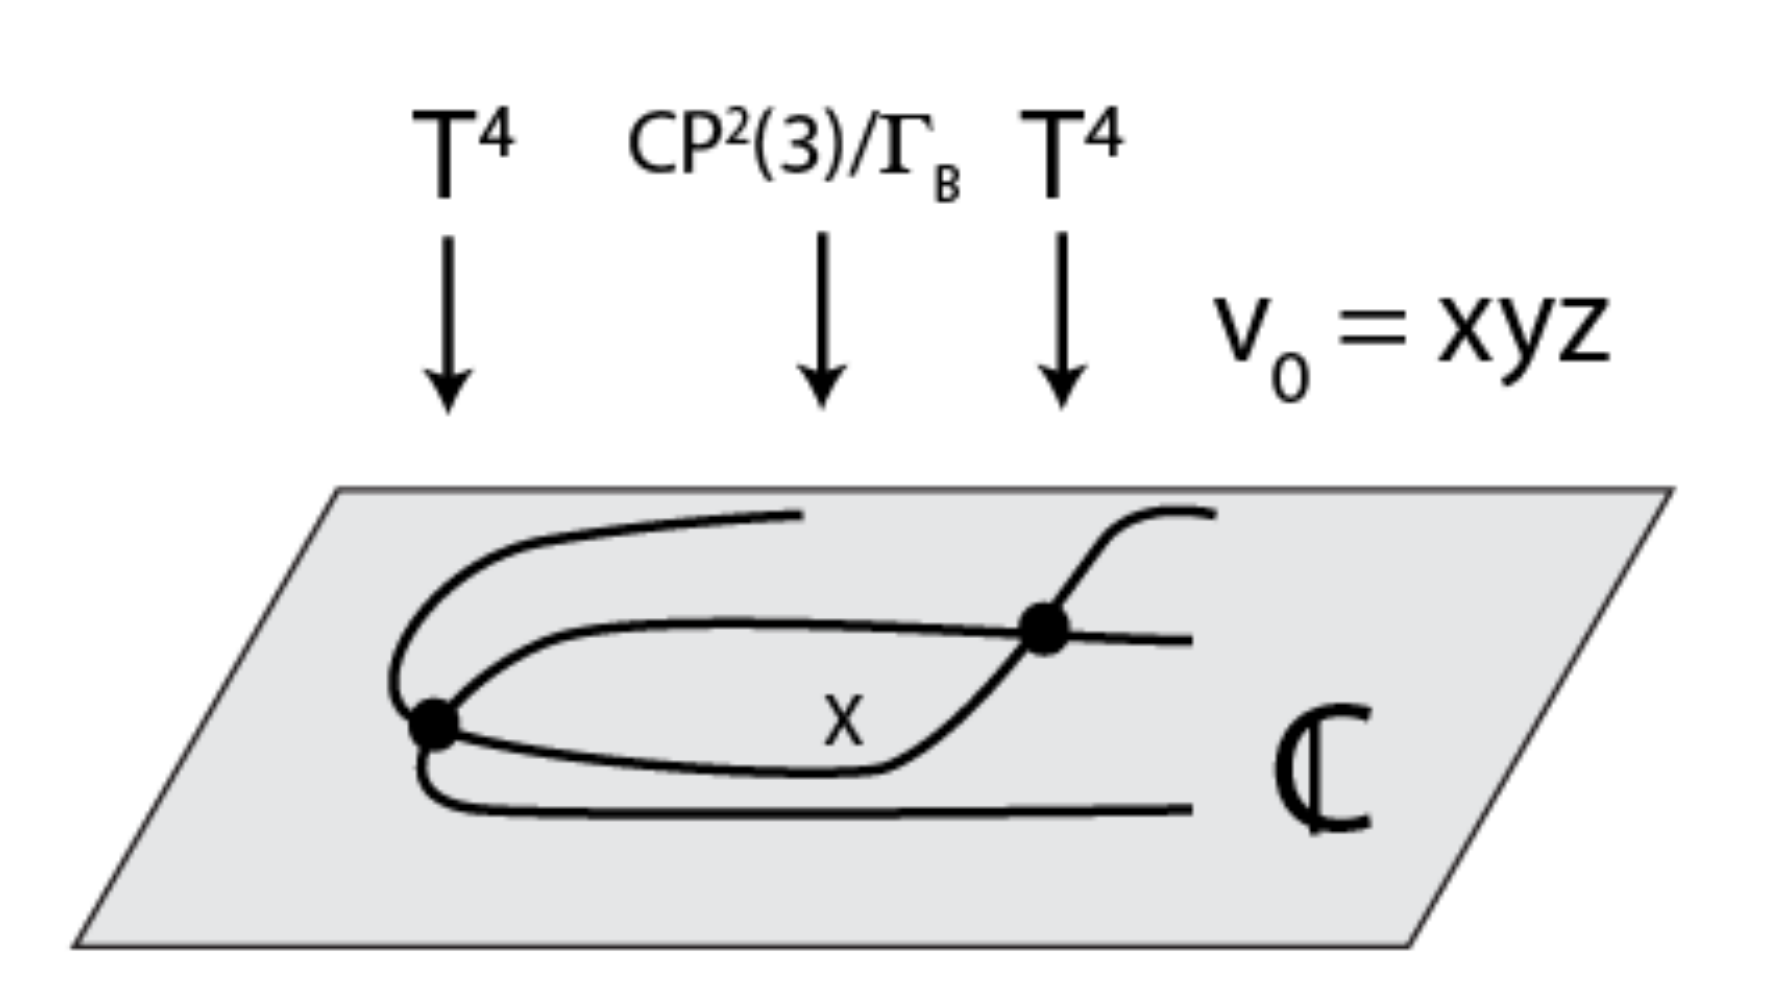
\includegraphics[width=0.64\textwidth]{figures/fig_4_5.png}
\caption{$L_i$：把 $\ell_i$ 沿 $v_0$ 底空间中的 U 形曲线平行移动（原书 p.111）}
\label{c8:fig-Li}
\end{figure}

\transnote{对象的「纤维化」要求是本文与 [Sei08] 的关键差别。这里只允许沿 U 形曲线平行移动所得的拉格朗日，它们在紧集之外投影成射线；正因为如此，才能像式~\eqref{c8:eq-hom} 那样按射线的上下位置定义一个序，而不必先做 Hamilton 扰动。}

\begin{lemma}\label{c8:lem-hom-position}
局部化范畴中 hom 的落位正确；论证见 Abouzaid--Seidel、Ganatra 的笔记与 Abouzaid--Auroux。
\end{lemma}

\begin{lemma}\label{c8:lem-roof}
roofs 的复合仍是 roof。
\end{lemma}

\begin{proof}
参见 M. Jeffs 的硕士论文。
\end{proof}

\transnote{读 roof 时注意箭头的方向与谁是拟同构。$K<L$ 时，先沿推射线把 $K$ 抬成 $K^\eps$，使它高于 $L$；此时按式~\eqref{c8:eq-hom}，$K^\eps\to L$ 才有定义（因为 $K^\eps>L$），而 $K\to K^\eps$ 是拟同构。原文说「形式地反转态射」，指的就是把本不存在的 $K\to L$ 用这条 roof 来表达。}

% ===== 原书 p.112 =====

\begin{remark}[单位]\label{c8:rem-units}
在 Floer 理论中 $\mathrm{HF}(V,V)\cong H(V;\KK/2)$。
$2$-环面（$T^4$ 纤维中「高度为零」的部分）的上同调环：$0$ 次与 $2$ 次为 $\Z$，$1$ 次由 Künneth 公式为 $\Z\oplus\Z$。
上链层面的生成元个数确实相同。
\end{remark}

\transnote{$\KK/2$ 不是把系数域除以 $2$，而是半整数分次：单位所在的次数可以落在 $\frac12\Z$ 里。对照下一句「上链层面生成元个数相同」，作者是在说：$V$ 的上同调按 $\Z$ 分次算出的生成元，与按 $\frac12\Z$ 分次算出的相同。}

\begin{definition}\label{c8:def-donaldson-fukaya}
Donaldson--Fukaya 范畴：对态射链复形取上同调即得。
它是拓扑量子场论的一个例子，即从流形到向量空间、把配边映到向量空间同态的函子。
\end{definition}

\begin{lemma}\label{c8:lem-J-indep}
设 $J_1$ 与 $J_2$ 是两个正则近复结构，则它们给出拟等价的 Fukaya $A_\infty$-范畴。
\end{lemma}

\begin{proof}
见 Seidel §8 与 §(10c)。
\end{proof}

\transnote{「拟等价」与「拟同构」要分清：两个范畴之间的 $A_\infty$ 函子若每个态射复形上都诱导拟同构，就称拟等价；两个对象之间的态射若在同调上诱导同构，才叫拟同构。本条的结论是在范畴层面说的，故用「拟等价」。}

\begin{remark}\label{c8:rem-indep-discussion}
[Sei08] 的 (10a) 与 (10b) 讨论了这件事，但超出我们的需要。[Sei08] 的 (10c) 含 Donaldson--Fukaya 范畴同构的论证。

我们可以构造一个 $A_\infty$ 函子（如前所述，它就是恒等），见 [Sei08] 开头；于是不必考虑同伦。
一般情形下这不对，因为 $\mu^2$ 可能跳；但这里不会，因为所有交点都在 $0$ 次。
我们有线性的连续映射，高阶的都是恒等。

FOOO 与 Floer 的经典做法是构造同伦。见 [FOOO09a, p 244]：同伦的代数背景在第 4.2 节；引入虚拟基本链之后，定理用于 Fukaya 范畴情形，见该书 Corollary 4.6.3 或他们 2000 年预印本的 Theorem 15.19。

Seidel 把 $J$ 的各选择所对应的所有 Fukaya 范畴打包成一个「总」Fukaya 范畴，从而把这一套升级到 $A_\infty$ 情形。
他证明每个 $\cF(Y)_i$ 都全忠实嵌入总范畴，并借助 Salamon--Zehnder 对实际范畴的工作，在上同调上诱导同构。
于是所有 $\cF(Y)_i$ 都拟同构于同一个对象，从而彼此拟同构，证明完成。

注意，[FOOO09a, p 244] 讨论了 $J$-不变性。代数同伦不变性在第 4.2 节讨论，主定理在第 4.6 节。
两者之间，他们把几何基本链搭成第 4.2 节代数理论的一个应用。

一般地，用单个 PDE 在两个 $J$ 之间插值的连续映射论证，给出每个选择下 Floer 群的同构；Seidel 在 [Sei08, §(10c)] 讨论了如何把它升级到 $A_\infty$-范畴。
\end{remark}

\transnote{这里说「不必考虑同伦」，前提是所有交点都在 $0$ 次，故 $\mu^2$ 不会跳。一般情形下 $\mu^2$ 是可能跳的，那时必须像 FOOO 与 Floer 那样显式构造同伦；原文特意点出这一点，读者不要把它当成普遍结论。}

% ===== 原书 p.113 =====

\begin{corollary}\label{c8:cor-well-defined}
此范畴与正则数据的选择无关，故良定义。
特别地，足够小的不同 $T$ 值给出拟同构的 Fukaya 范畴——定义复结构时 $\Gamma_B$ 有可商的正纯全纯群作用。
\end{corollary}

\begin{proof}
对正则 $J$ 的不变性已如上。纤维中 Hamilton 扰动下的不变性，文献中已有。
这就完成了「良定义的 Fukaya 范畴」的证明。
\end{proof}

\begin{remark}\label{c8:rem-family}
技术上，我们会有一个 $T$ 上一族 Fukaya 范畴之间的镜像对应，故复结构 $J_T$ 涉及缩放标准 $J$，并缩放 A 侧的辛形式。
要证不变性，得看近复结构空间中的一条连通路径，即缩放这个 $T$ 所得的路径。
\end{remark}

\transnote{最后这条注把视野放大到 $T$ 上的整族范畴。$T$ 是复结构的参数，缩放 $T$ 同时缩放两侧：$B$ 侧的复结构、$A$ 侧的辛形式。原文说「看近复结构空间中的连通路径」，就是要在缩放过程中逐点比较范畴，而不是孤立地比两个 $T$ 值。}

\transnote{本块收束第 4 章。原书把「不依赖选择」这件事分成两层：正则 $J$ 的选择，与纤维中 Hamilton 扰动的选择。前者靠上一节的 Sard--Smale 与模空间理论，后者在文献里已有；两者合起来才得到良定义的 $H^0(FS(Y,v_0))$。}

% EN48 c09 | 原书 p.114–130（PDF 123–139） | 第 5 章 §5.1–5.2
% 骨架文件：标题行已设定，正文由译者填写。每页起首用 % ===== 原书 p.N ===== 注释标记。
\section{主定理}

\subsection{HMS 计算}

% ===== 原书 p.114 =====
\begin{remark}\label{rem:tqft}
在物理中，函子 $(Y,v_0)\mapsto H^0(\mathrm{FS}(Y,v_0))$ 可称为\emph{拓扑量子场论}（topological quantum field theory），简称 TQFT。也就是说，TQFT 的第一部分是从某些流形到向量空间的函子。更多背景可见 Segal 的讲义 [Seg]。本文考虑的是 Donaldson--Fukaya 范畴，完整的 $A_\infty$-范畴等价是未来的方向。要过渡到 $H^0$，我们需要知道微分。
\end{remark}

\begin{remark}\label{rem:diff}
回忆上文给出的 Fukaya--Seidel 范畴的定义。然而，要在上同调层面证明全忠实的 HMS 嵌入，我们需要计算 $\mathrm{FS}(Y,v_0)$ 上的微分，以求出 $H^0(\mathrm{FS}(Y,v_0))$ 中的态射群；仅知道微分存在还不够。此外，上文的定义使用正则 $J$，排除了球泡（sphere bubbling）；这一结论来自对 McDuff--Salamon 结果的改造。其哲学是：假设「一般的 $J$」对应「一般相交」中的一般性，则 0 维球族中所有点之并为两点，1 维圆盘族中所有点之并为三点；因此在 6 维流形中，二者一般不相交。
\end{remark}

然而，下文计算微分时我们使用标准 $J_0$，即环面坐标中乘以 $i$ 的复结构。此时无法排除球泡。原因在于 $H_2(v_0^{-1}(0))$ 非平凡：$v_0^{-1}(0)$ 是 $Y$ 的中心纤维，它来自 $J_0$-复子流形，因为 $v_0$ 关于 $J_0$ 全纯。非零的 Dolbeault 上同调说明这些球不正则；具体说，由 Riemann--Roch，$\bar\partial$ 算子的余核正是 Dolbeault 上同调。我们用 Gromov--Witten 不变量理论描述 [KL19] 中给出的球计算；再用 polyfold 理论对 $\bar\partial_J$ 作抽象扰动 [BFW17]，说明非正则 $J$ 下 Fukaya 范畴不变。于是 polyfold 给出的 Fukaya 范畴，与直接用 $J_0$ 算出的范畴拟同构。

\transnote{这里的要害是：正则性只对「一般的 $J$」成立，而 $J_0$ 是特殊的复结构。$J_0$ 下出现的全纯球并不正则，因此不能把它们当作 $J$-全纯曲线来数；作者改用 polyfold 的抽象扰动绕开这一点。阅读下文时，凡出现 $J_0$ 的计算，都应理解为「先对 $J$ 计数，再取极限」。}

% ===== 原书 p.115 =====
于是，用 $J_0$ 直接计算微分，即可把 HMS 两边的范畴对应起来。

\begin{remark}[记号]\label{rem:notation-M}
大写 $M^k$ 表示 $Y$ 全空间上的结构映射；小写 $M^k$ 表示环面纤维上的结构映射。
\end{remark}

\begin{lemma}\label{lem:compute-d}
$\partial:CF(\ell_{i+1},\ell_j)[-1]\to CF(\ell_i,\ell_j)$ 可由全体 $z$ 的 $\partial:CF(t_z,\ell_i)\to CF(t_z,\ell_i)$ 数据算出。
\end{lemma}

\begin{proof}
设 $p_j$ 为 $\ell_j$ 与 $t_z$ 的交点；设 $t^k_{i,j}$ 为 $\ell_i\cap\ell_j$ 的第 $k$ 个交点，其中 $0\le k<(i-j)^2$，如上面 Fukaya--Seidel 范畴定义所述。下图的第一与最末竖直箭头可以算出，我们要算中间的箭头。设微分把 $p_j$ 送到 $C(z)\cdot p_j$；这里 $C(z)$（count）是一个待计算的计数，它依赖 $z$ 而不依赖 $j$。这个图让我们求出中间的竖直箭头。注意：大写指沿底空间中的曲线平行移动小写纤维拉格朗日。论证的关键是 Leibniz 法则。见图 5.1。
\[
\begin{tikzcd}[column sep=2.8em, row sep=3.4em]
\hom(\ell_j,t_z)\otimes\hom(\ell_{i+1},\ell_j)\ni p_j\otimes t^k_{i+1,j}
  \arrow[r,"M^2"] \arrow[d,"\partial"'] &
\hom(\ell_{i+1},t_z)\ni M^2(p_j,t^k_{i+1,j}) \arrow[d,"\partial"] \\
\hom(\ell_j,t_z)\otimes\hom(\ell_i,\ell_j)\ni C p_j\otimes\partial(t^k_{i+1,j})
  \arrow[r,"M^2"'] &
\hom(\ell_{i+1},t_z)\ni \partial(M^2(p_j,t^k_{i+1,j}))
\end{tikzcd}
\]

特别地，由乘积求导的 Leibniz 法则，有
\[
M^1(M^2(p_j,t^k_{i+1,j}))
=M^2(M^1(t^k_{i+1,j}),p_j)+M^2(t^k_{i+1,j},M^1(p_j))
=M^2(M^1(t^k_{i+1,j}),p_j),
\]
因为 $M^1(p_j)=0$：$p_j$ 的次数为 0，而两拉格朗日的其他交点处没有 1 次元；注意 $p_i$ 的次数为 $-1$。注意 $M^1(t^k_{i+1,j})$ 正是我们要求的对象。又因在米色区域纤维丛平凡，可在纤维中数以 $p_i,p_j,t^k_{i+1,j}$ 为顶点的三角形，得 $M^2(p_j,t^k_{i+1,j})=D(z)\cdot p_i$，其中 $D(z)$ 是某个函数。再由同伦论证算得 $M^1(p_i)=C(z)\cdot p_j$。于是上式给出
\[
C(z)\cdot D(z)\cdot p_j=M^2(M^1(t^k_{i+1,j}),p_j),
\]
由此可算出 $M^1(t^k_{i+1,j})$。
\end{proof}

\transnote{图中两行并不是两个独立命题：上排是「按定义」的一侧，下排是「按计算」的一侧。竖直箭头 $\partial$ 把上排元素送到下排，横向的 $M^2$ 是乘积。作者先算出首末两条竖直箭头，再用交换性反求中间一条。读图时注意 $M^2$ 的两个自变量顺序：在 $M^2(p_j,t^k_{i+1,j})$ 中 $p_j$ 在前。}

\transnote{$M^1(p_j)=0$ 的理由是次数：$p_j$ 是 0 次交点，而同处没有 1 次交点，故微分的 0 次分量作用在 $p_j$ 上为零。相对地，$p_i$ 的次数为 $-1$，所以 $M^1(p_i)$ 不必为零。这一处最易把 $p_i$ 与 $p_j$ 的次数记反。}

我们愿意用 $t_z$ 而不用某个 $\ell_j$，是因为这样可以数边界落在矩映射原像中的圆盘，如 [CO06]。把 $t_z$ 沿 U 形曲线平行移动得到的拉格朗日 $T_z$，对应镜像侧点 $z$ 处的赋值截面。因此，一旦知道全体 $t_z$ 的态射群，就知道了任意 $\ell_i$ 与 $\ell_j$ 之间的 hom。

% ===== 原书 p.116 =====
\begin{figure}[!htbp]
\centering
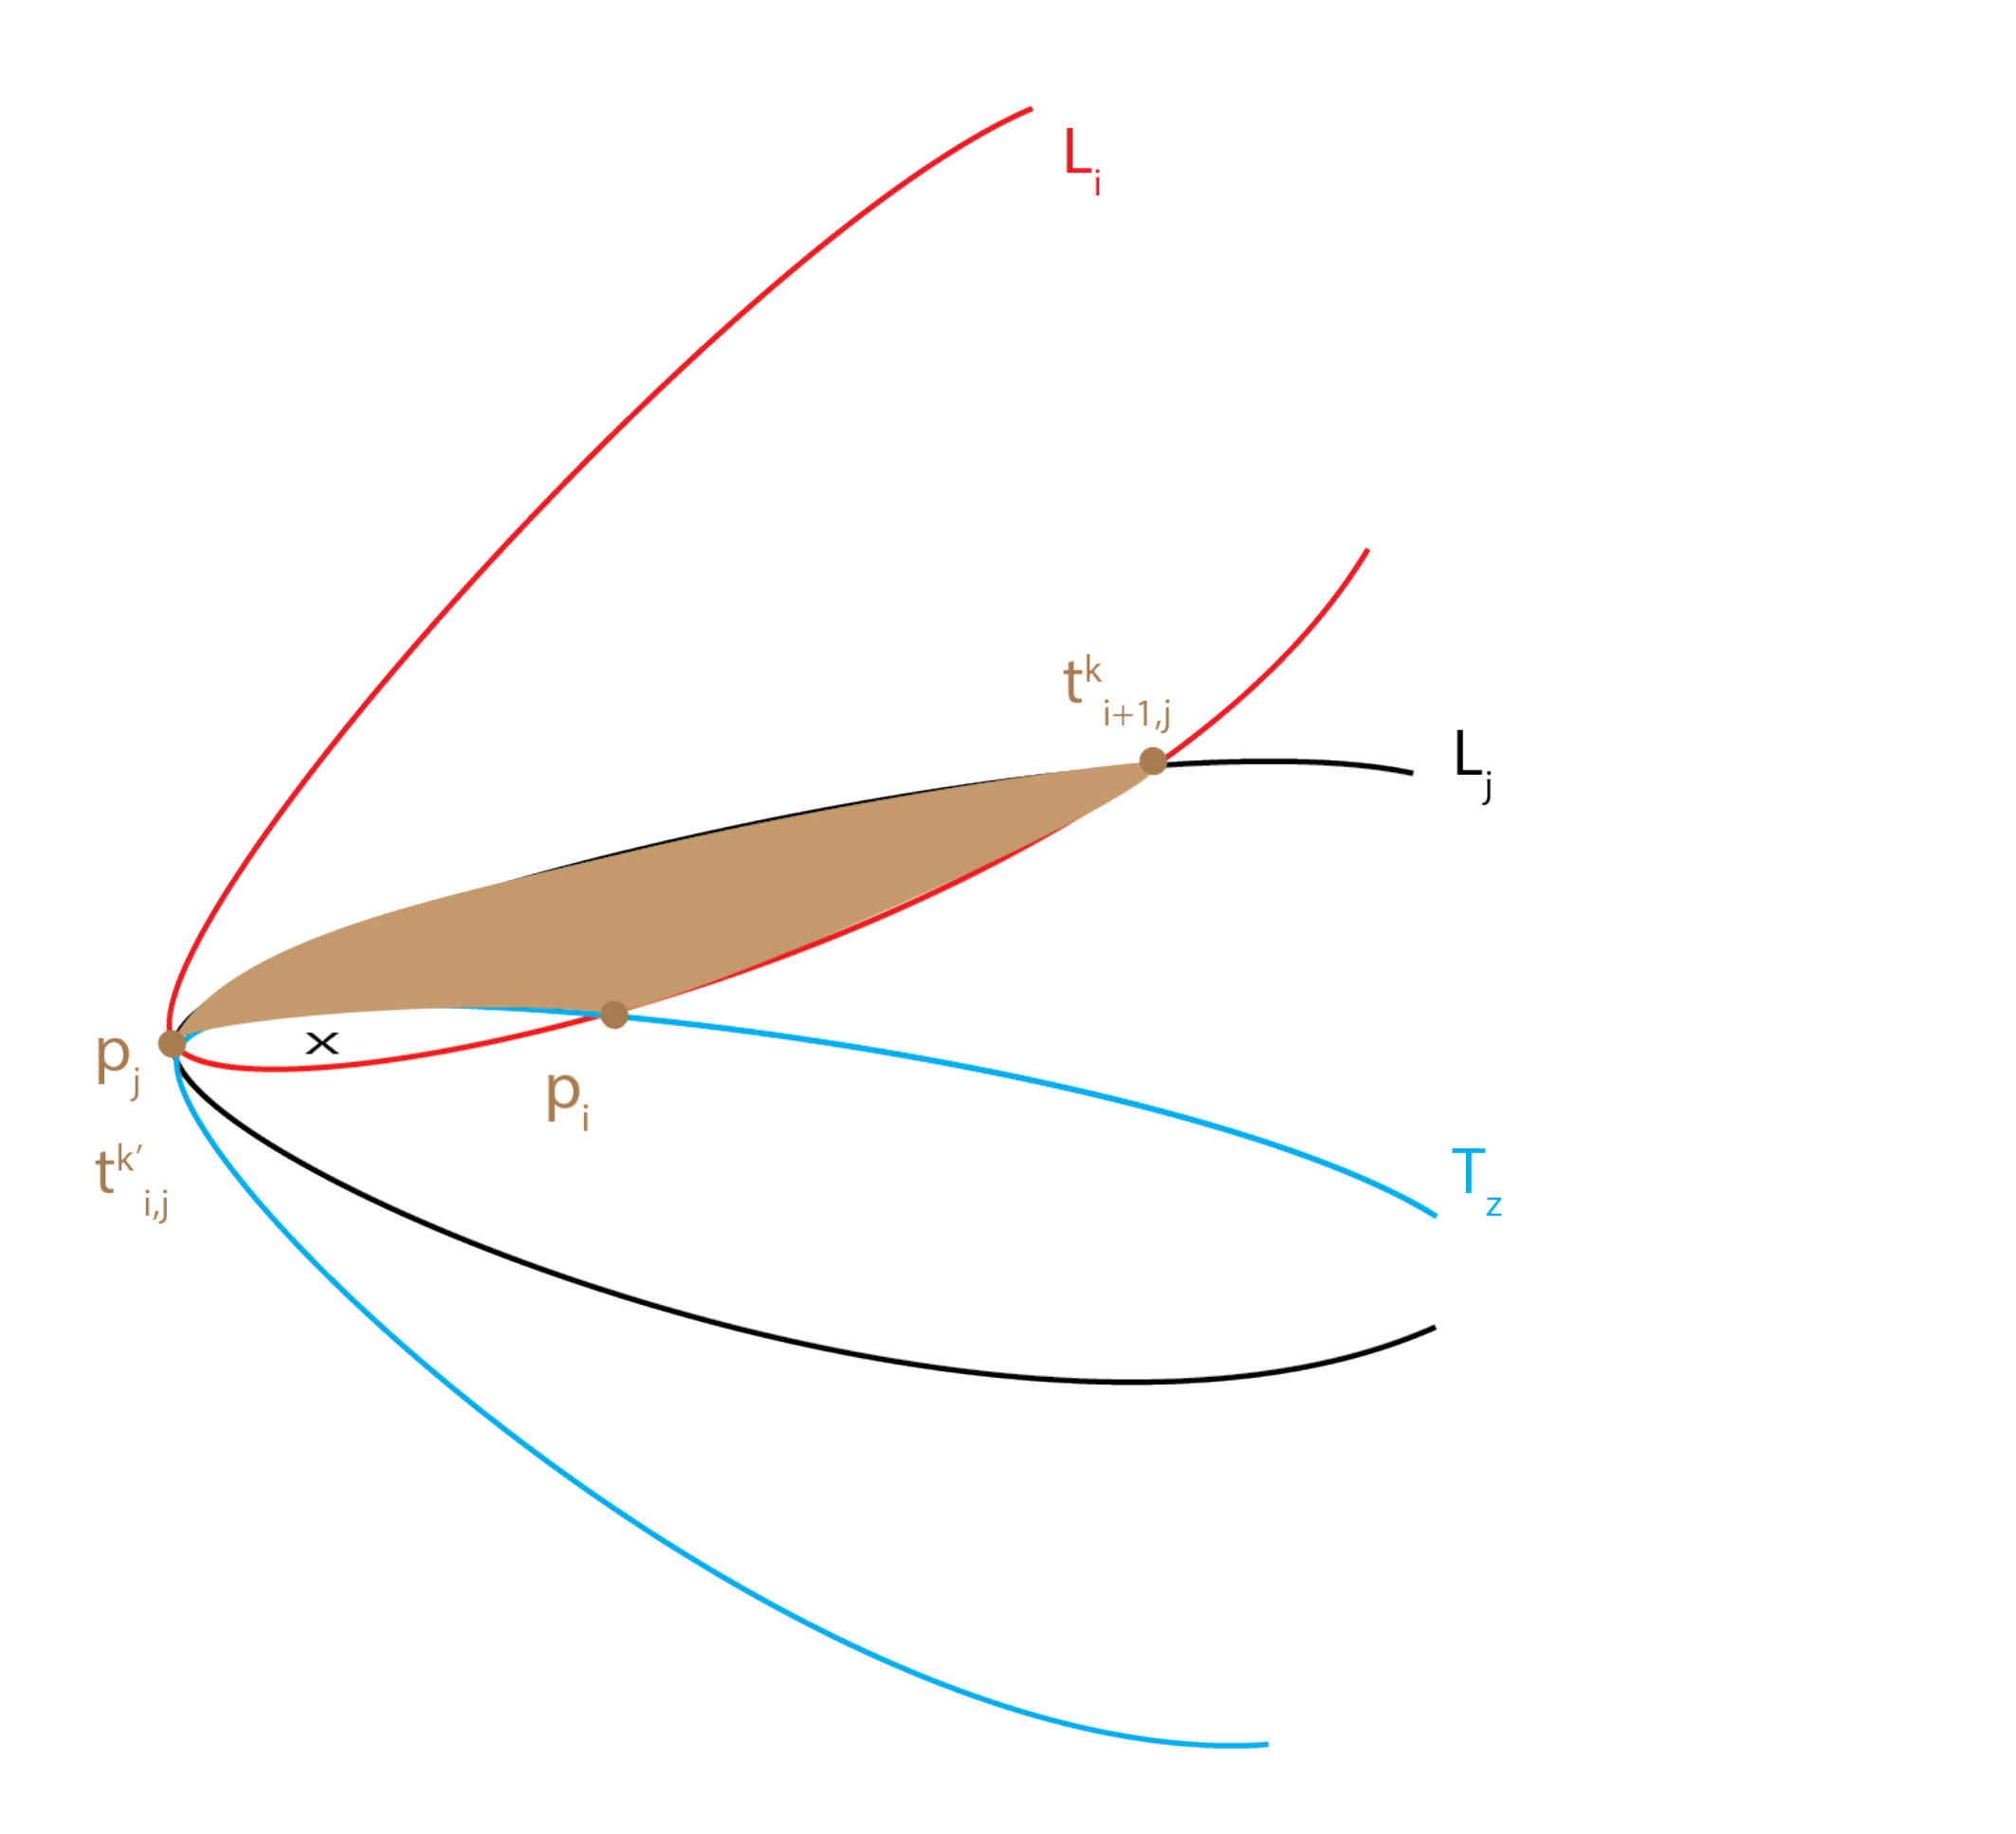
\includegraphics[width=0.40\textwidth]{figures/fig_5_1.png}
\caption{Leibniz 法则（原书 p.116）}\label{fig:leibniz}
\end{figure}

下面描述同伦论证，它将使我们求出 $M^1(p_i)$。见图 5.2 与 5.3。

\begin{figure}[!htbp]
\centering
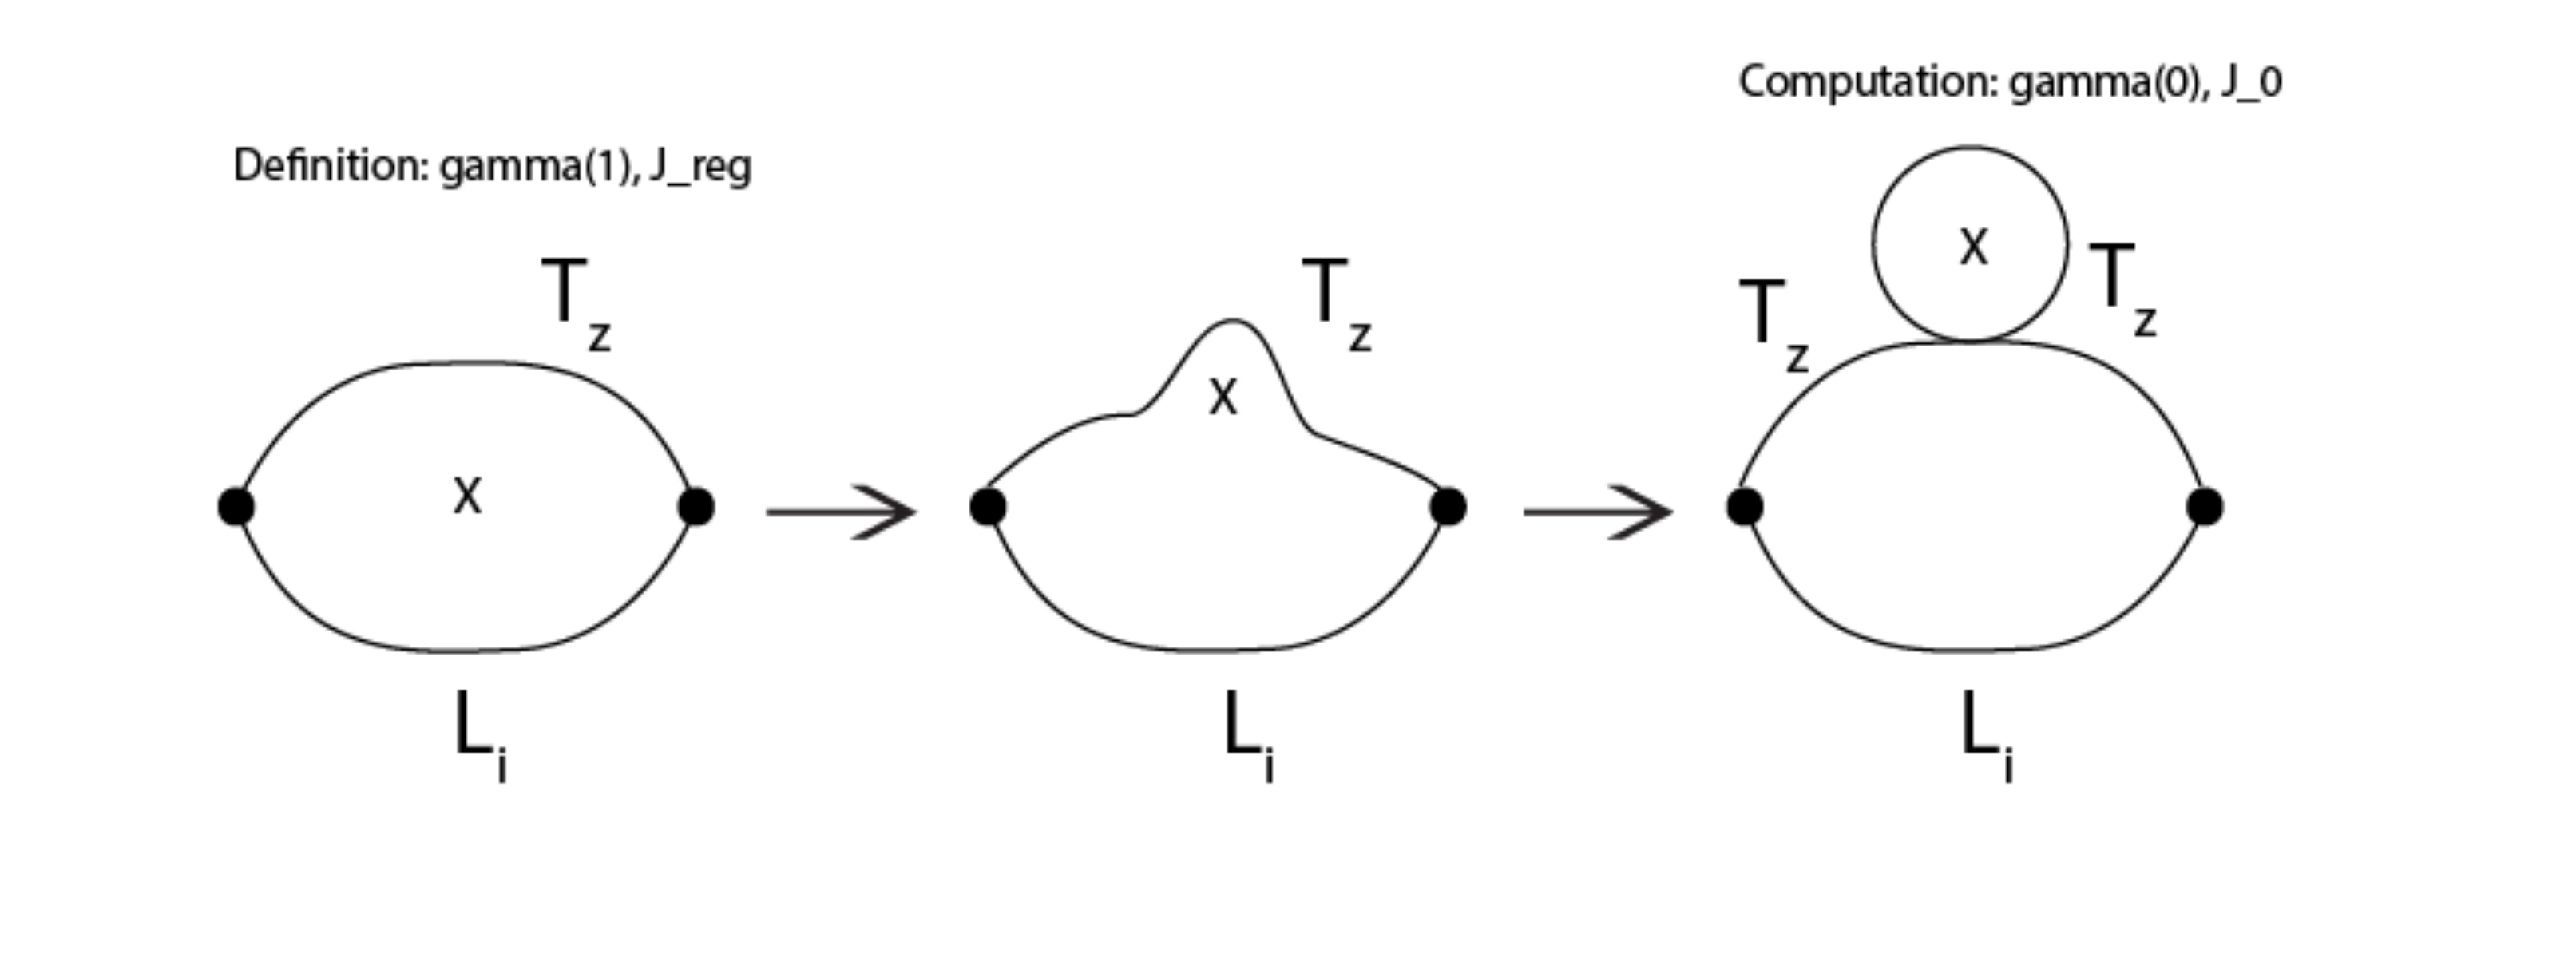
\includegraphics[width=0.84\textwidth]{figures/fig_5_2.png}
\caption{$\partial$（左）与我们所计算的圆盘计数（右）之间的同伦（原书 p.116）}\label{fig:homotopy}
\end{figure}

\transnote{图 5.2 左边标着「Definition: gamma(1), J\_reg」，右边标着「Computation: gamma(0), J\_0」。左图是定义侧：$T_z$ 与 $L_i$ 之间夹一个圆盘 $x$。右图是计算侧：同一圆盘在 $r=0$ 处多出一个球泡。两者之间的箭头表示同伦，而不是相等。}

\begin{remark}\label{rem:abstract-perturb}
用 $J_0$ 计算时，我们使用的是非正则 $J$。因此需要一套关于 $J$ 的不变性论证，它要涵盖非正则 $J$ 下的不变性。为此我们采用 polyfold 的抽象正则化方法：用 Banach 丛的一个截面扰动 $\bar\partial_{J_0}$；该截面未必由扰动 $J_0$ 诱导，故称「抽象」。
\end{remark}

[KL19] 中 Gromov--Witten 不变量的计算，需要证明开 Gromov--Witten 与闭 Gromov--Witten 具有同构的 Kuranishi 结构；

% ===== 原书 p.117 =====
\begin{figure}[!htbp]
\centering
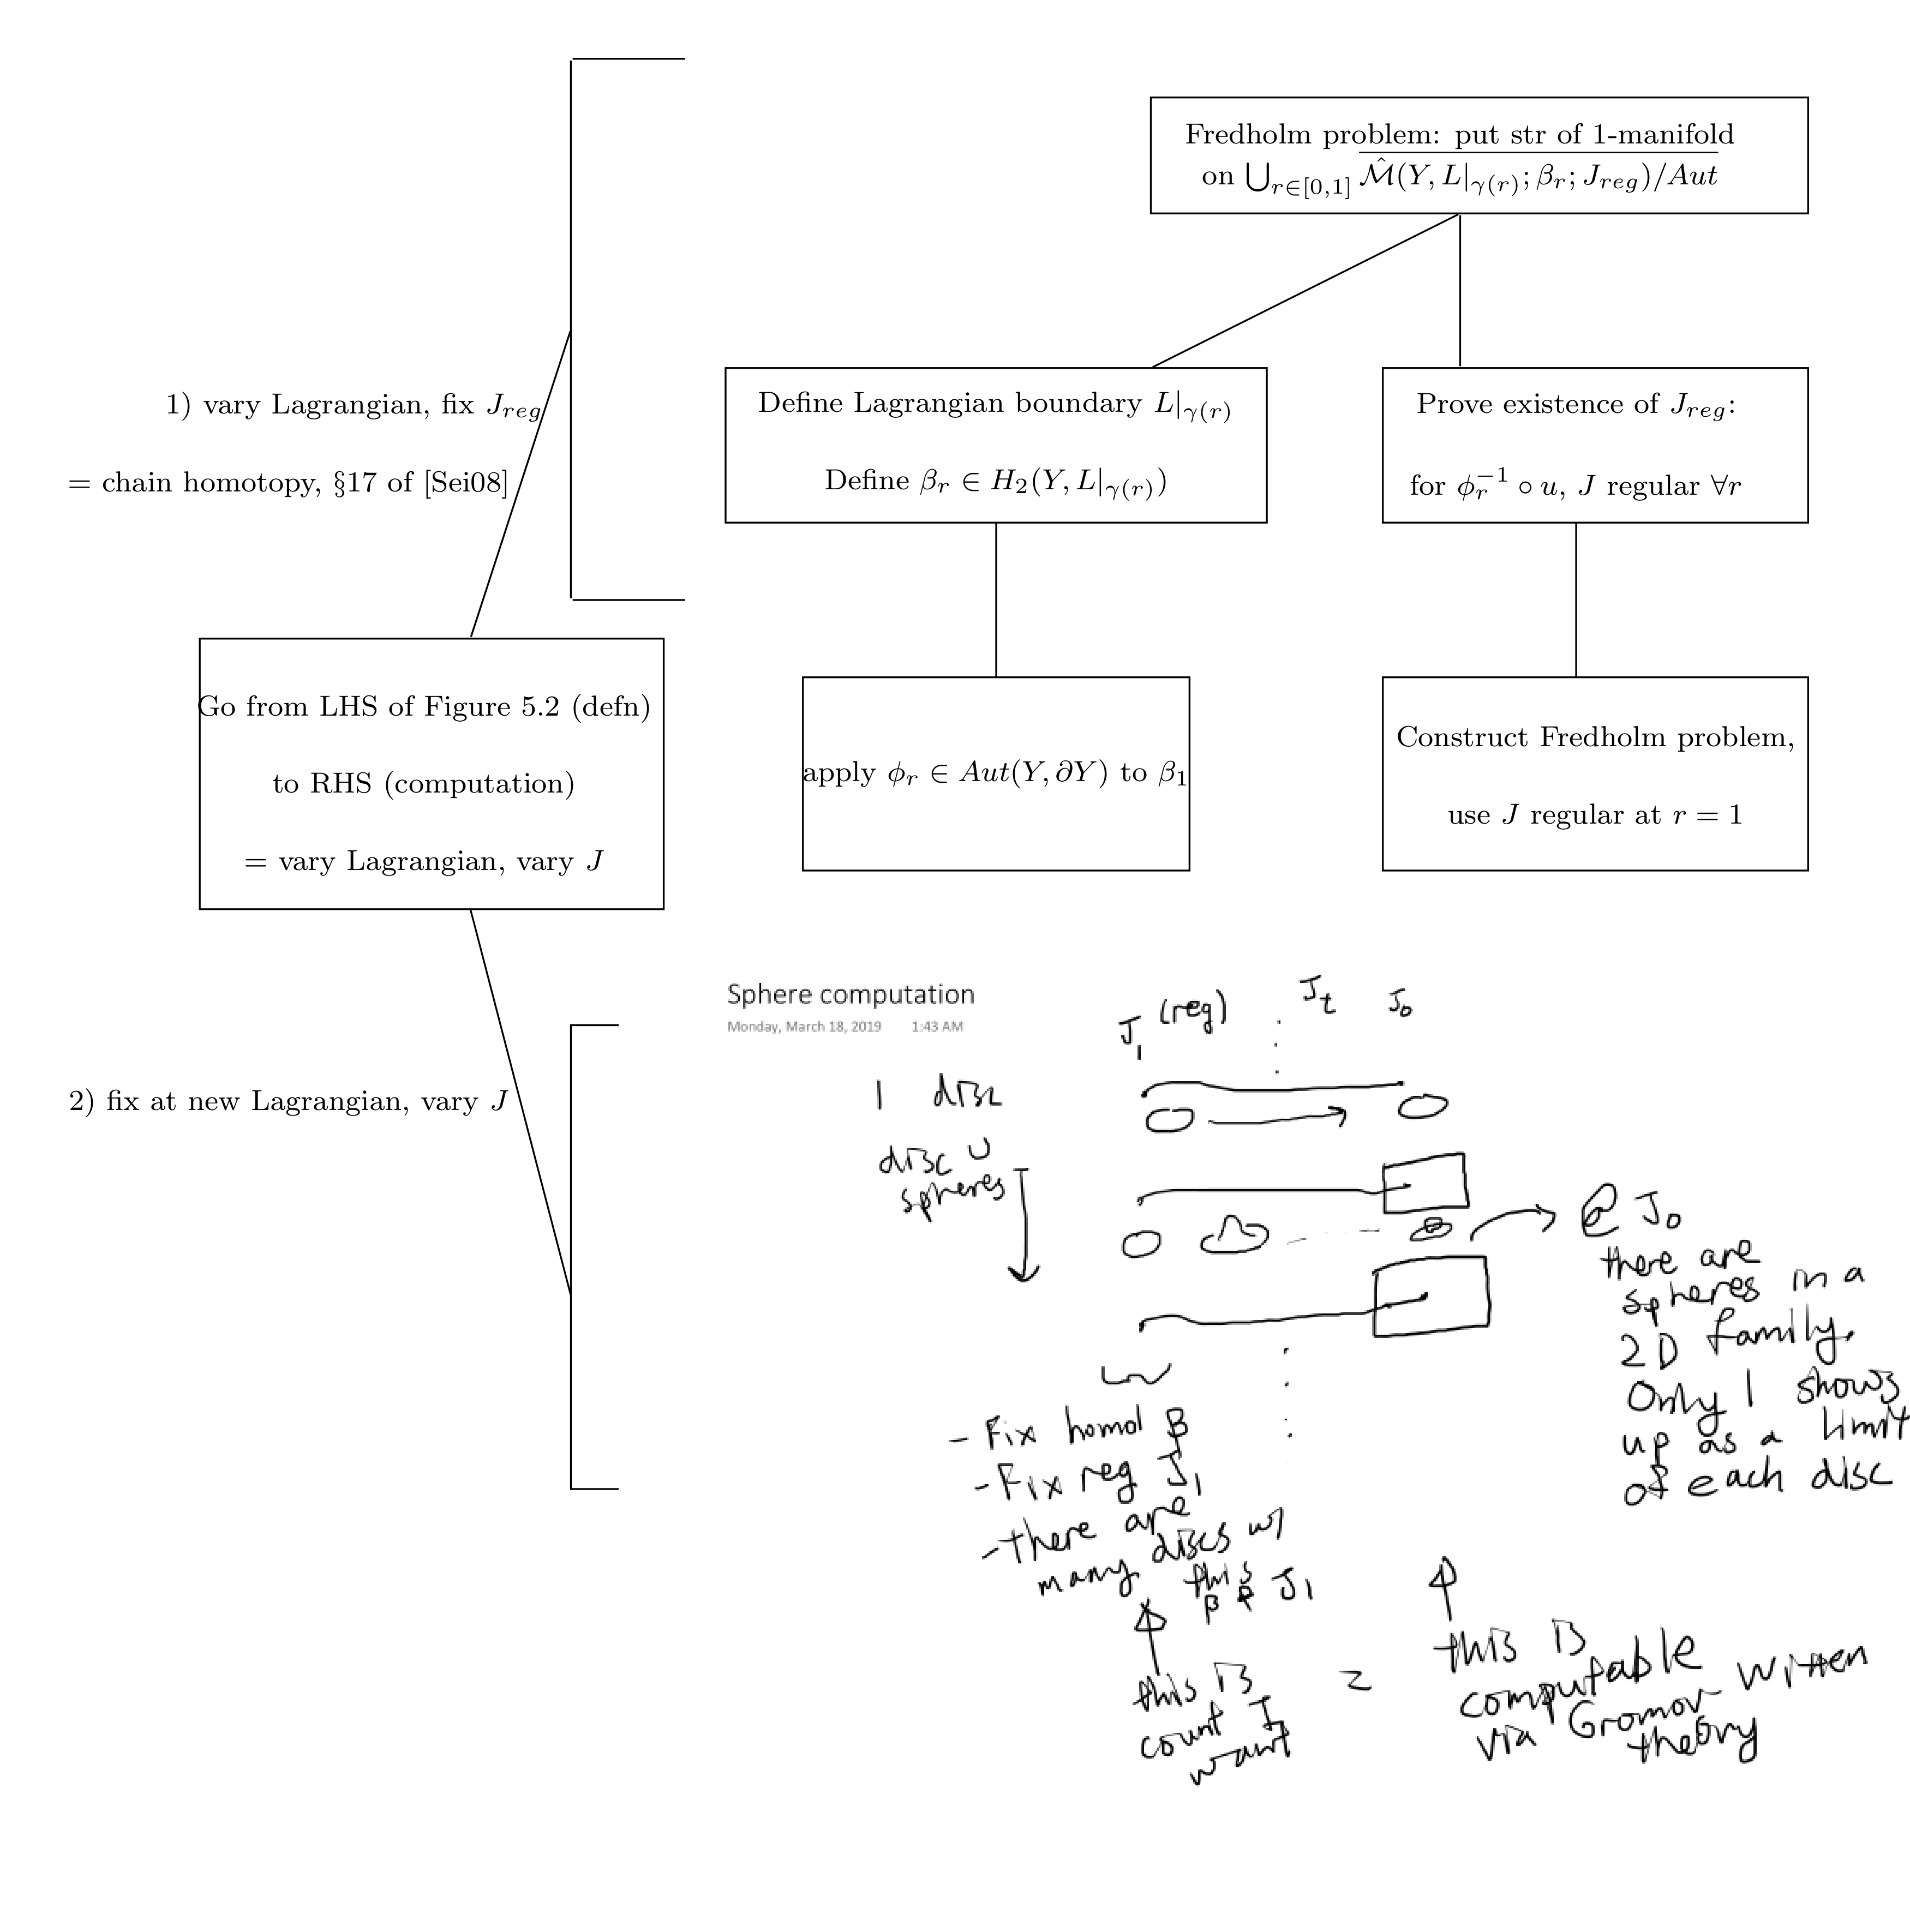
\includegraphics[width=0.46\textwidth]{figures/fig_5_3.png}
\caption{计算计划（原书 p.117）}\label{fig:plan}
\end{figure}

\transnote{图 5.3 是作者手写的流程图，页面上没有可排版的正文。图中左侧是两条路线：1）变拉格朗日、固定 $J_{reg}$；2）在新拉格朗日处固定，变 $J$。右侧上方是从 $J_{reg}$ 到 $J_0$ 的 Fredholm 问题构造，下方手写部分是球泡计算的草稿。中间的 $\widehat{\mathcal{M}}(Y,L|_{\gamma(r)};\beta_r;J_{reg})$ 表示带 $r$ 参数族的模空间。}

% ===== 原书 p.118 =====
这一点用到 [Cha11]，下文还会讨论。本节先讨论同伦论证；然后讨论圆盘与球泡的计算；最后用 polyfold 论证说明计算与定义的关系。

\begin{remark}[记号]\label{rem:notation-seidel}
本节使用 [Sei08, §17g] 中发展起来的理论，用于数穿过奇异纤维的伪全纯多边形截面。在该节中，$d$ 在这里称为 $M^1$。Seidel 的 $L_1,L_2$ 在本设定中为 $t_z$，且 $Q=\ell_i$；这由 $L_2$ 同痕于 $\phi(L_1)$ 得到。此处的其他映射应与 Seidel 的记号同名。
\end{remark}

\transnote{读本节必须同时翻开 [Sei08, §17g]。那里的 $d$ 是微分，此处改称 $M^1$；那里的 $L_1,L_2$ 是拉格朗日，此处是环面纤维 $t_z$；那里的 $Q$ 此处是 $\ell_i$。作者只保留了结构，不保留字母，稍不留神就会把两套记号混在一起。}

\begin{lemma}\label{lem:M1-homotopic}
$M^1:CF(T_z,L_i)\to CF(T_z,L_i)$ 同伦于 $M^2(c,-)$，其中 $c$ 是圆盘计数乘以合适的交点 $p$。
\end{lemma}

\begin{proof}
首先注意
\[
M^1:CF(t_z,\ell_i)\to CF(t_z,\phi(\ell_i))
\xrightarrow[\phi^{-1}]{C}F(\phi^{-1}(t_z),\ell_i)=CF(t_z,\ell_i)\cong\C,
\]
其中 $\phi$ 是单值性。这里用到：微分同胚 $\phi^{-1}$ 给出交点之间的双射；而 $t_z$ 在平行移动下不变，因为它只旋转角度。于是得到 $CF(t_z,\ell_i)$，而它只有一个交点。

开 Gromov--Witten 不变量理论可以数 $J_0$-全纯圆盘：边界在矩映射纤维上，有一个标记点，并且穿过 $Y$ 的奇异纤维一次（确实如此，因为按定义它们是 1-1 的，且在 $J_0$ 下实际得到 $v_0$ 的截面）。然而，$M^1$ 按定义是在 $T_z$ 与 $L_i$ 上边界、穿过奇异纤维的 bigon 计数。于是仿照 [Sei08, §17g]，我们形变 $M^1$。把边界在 $T_z$、标记点为 $p$ 的 $J_0$-全纯圆盘计数记为 $c\cdot p$。该形变构造同伦 $l$，使
\[
M^2(c,\cdot)-M^1(\cdot)=M^1\circ l-l\circ M^1=0,
\]
其中为零是因为在环面纤维上 $M^1=0$。见图 5.2。下面我们叙述他书中的细节，并按本文略有不同的设定补足所需信息。在本设定中，Seidel 作 Dehn 扭转所对的 vanishing cycle，其类比是三族退化为交于一点的 $S^1$ 的 $T^2$。不过，应用他的理论需要一条性质：单值性 $\phi$ 保持 $t_z=\{(\xi_1,\xi_2,\theta_1,\theta_2)\}_{\theta_1,\theta_2\in[0,2\pi)}$；这一点在这里仍成立。

我们先定义 $k$，它是 $\tilde d:=M^2(c,-)$ 与零映射之间的同伦；这里 $c$ 是闭的，从而是 Floer 同调的代表类。令 $\tilde l=M^2(k(\cdot),\cdot)+M^3(c,\cdot,\cdot)$。
\end{proof}

\begin{claim}\label{claim:boxed}
$(\tilde d,\tilde l)$ 满足 [Sei08, (17.15)] 中的框内方程；这些方程表示 $\tilde d$ 是纤维上两个 $CF$ 群之间的链映射，而 $\tilde l$ 是 $\tilde d\circ M^2$ 到零的同伦。
\end{claim}

此外，同痕 $L_1,L_2$，并取满足同一组方程的不同 $(d,l)$ 选择，所得映射彼此同伦。因此有唯一性陈述；取选择的极限不改变理论。

% ===== 原书 p.119 =====
\begin{proof}
方程 (17.15) 由 $(\tilde d,\tilde l)$ 的定义即得满足。下面看 $(d,l)$ 如何依赖 $L_1$，带 tilde 的情形同理。用 continuation maps $a$ 与 $b$，分别从 $CF(Q,L_1)$、$CF(L_0,L_1)$ 走到 tilde 版本。于是这些映射良定义，即输入相同。Seidel 还断言：continuation maps 与三角积相容，至多差一个链同伦。continuation maps 的模空间中的映射，其边界条件在 $Q$ 或 $L_1$ 上为常值，并在条状端的时间 1 侧实现 $L_1$ 到 $\tilde L_1$ 的同痕。三角积相容性所需链同伦 $h$ 的模空间如下：取边界为 $Q,L_0,L_1$ 的平凡纤维丛，粘上 $a$ 的模空间；对 $(Q,L_0,\tilde L_1)$ 同样做，粘上 $b$。链同伦 $h$ 定义为在这两者之间。由于 continuation maps 是拟同构，上同调上得到同构。同样，同痕 $L_2$ 仍得上同调同构。

先看插值于 Floer 复形之间的模空间。具体说，$\delta$ 是两端交点 $t_z\cap\ell_i$ 上两个 Floer 复形之间的映射；$\lambda$ 是积映射。新对象 $\delta,\lambda$ 满足与 (17.15) 类似的方程，但分别多出 $d+\tilde d$ 与 $l+\tilde l$ 项。这些方程说的是：链复形 $C'\oplus C\oplus C''$ 与 tilde 版本同构。注意 $(\delta,\lambda)$ 是更一般地变 $(\tilde d,\tilde l)$ 的构造；而 $(\alpha,\beta)$ 是特别地通过变 $L_1$ 来变 $d$ 的构造，后者比前者引入更多项。

再看为何满足 (17.15) 的不同 $(d,l)$ 选择给出同伦的结果（这比「同痕 $L_1,L_2$ 得到不同选择」更一般）。取这样的 $(d,l)$。我们构造 $d$ 与 $\tilde d\circ a$ 之间的同伦，记为 $\alpha$；同样，记 $\beta$ 为 $l$ 与 $\tilde l$ 之间的链同伦。continuation maps 是拟同构，而 $\alpha,\beta$ 给出 $D$ 与 $\tilde D$ 之间的映射，它也是拟同构。
\end{proof}

\begin{claim}\label{claim:compute-M1}
我们可用 $M^2(c,-)$ 计算 $M^1$，并得到拟同构的 Fukaya 范畴。
\end{claim}

\begin{proof}
这是唯一性陈述的极限情形。这里 $\xi$ 与 $\psi$ 分别对应变微分与变乘积；$\xi$ 在 Seidel 所称的 $d$ 与 $M^2(c,-)$ 之间插值。我们取 $L_1$ 上同痕的极限。理由是：上一节正是这样变 $L_1$ 的，因此也正是这样变 $d$ 的。于是 $\tilde d$ 是上一节的极限情形，因为它是同痕 $\tilde L_1$ 的极限情形：这里 $\tilde d=M^2(c,-)$。
\end{proof}

% ===== 原书 p.120 =====
现在构造三角积的不同选择之间的同伦：考察一个由五部分组成的参数族。第一部分是原 $(d,l)$ 对中的 $l$。第二族关联于 $\xi(M^2)$：把 $\xi$ 纤维丛粘到一个平凡的 3 点圆盘。回忆 $\xi$ 是插值于两个「类微分」选项 $d$ 与 $M^2(c,-)$ 之间的 1 参数族。于是把这个族粘到 3 点圆盘上，又得到一个族。这样做实际上是把 $\xi$ 族变成作用于乘积层面的族。「大粘合长度」意味着它就是 $\xi(M^2)$。注意在 $r=0$ 处得到 $r=1$ 的 $l$ 族。在第二 $\xi$ 族的另一端，当 $r=1$ 时得到 $M^2(c,M^2(,))$。取足够大的闭区间 $[0;1]\subset\R^4$。
% [Tutor Note: 原文作 [0; 1] ⊂ R^4，与上下文不合；疑为 [0,1] ⊂ R 或 [0,1]^4 之误。译文保留原样，登记于报告。]

\transnote{原文此处作「$[0;1]\subset\R^4$」，分号与 $\R^4$ 都显得突兀。按上下文，作者只是要一个足够大的参数区间，故疑为 $[0,1]\subset\R$ 或 $[0,1]^4$ 的笔误。译文保留原样，未作改动。}

\begin{remark}\label{rem:gluing}
同伦的一侧有映射复合，即 $M^2(c,-)$。Fukaya 范畴中两个结构映射复合时，几何上对应把产生各自模空间的 Fredholm 问题粘起来。因此本设定下需要讨论粘合。这也是本设定与 Seidel 不同之处：书中他形变纤维丛；而此处丛不变，变的是拉格朗日边界条件。于是需要粘合论证，以推出模空间
\[
\bigcup_{r\in[0,1]}\mathcal{M}(J_{reg},L_r)
\]
是一维光滑流形。以下理论依照 [Weh14, Lecture 9]；另见 Wehrheim 2013 年秋季 topics 课程第 14 讲及 McDuff--Salamon：先用 $J_z$ 做，§10.9 处理只有 $J$ 的情形。
\end{remark}

\begin{claim}\label{claim:1dim}
$\displaystyle\bigcup_{r\in[0,1]}\mathcal{M}(J_{reg},L_r)$ 是 1 维流形。
\end{claim}

\begin{proof}[证明梗概]
为证光滑结构存在，构造一个 Fredholm 问题。设 $\gamma_r$ 为图 5.2 所示纤维丛底空间中的变动路径。设 $\{\phi_r\}_{r\in(0,1]}$ 是微分同胚的同痕
\[
\phi_r:(Y,L_i\cup T_z|_{\gamma_1})\xrightarrow{\cong}(Y,L_i\cup T_z|_{\gamma_r}),
\]
它在相应的相对第二同调群上诱导同构 $\phi_{r*}$。注意当 $r=1$ 时，用上面的方法已有曲线模空间的正则 $J$，且几何条件允许排除泡泡，于是得到紧的一维空间。这个 $J$ 又让我们定义一个 Banach 丛，作为 Fredholm 问题的底：
\[
\tilde{\mathcal{B}}^{k,p}:=\{(\phi_r^{-1}\circ u,r)\mid u:\R\times[0,1]\to(Y,L_i\cup T_z|_{\gamma_r})\in W^{k,p}\}.
\]
\end{proof}

% ===== 原书 p.121 =====
换一种说法，可把 $\tilde{\mathcal{B}}$ 中一条路径的切空间刻画为：路径在边界处的导数等于一个向量，该向量是拉格朗日边界切空间中的向量与同痕 $\phi_r$ 的流向量之和。由此，满足 $\bar\partial_J(\phi_r^{-1}\circ u)=0$ 的映射 $u$ 之集合得到 1 维流形结构，其中 $J$ 是上面定义的正则 $J$。

下一步在 $r=0$ 端作 Gromov 紧化。注意 $\phi_r$ 在 $r=0$ 处没有极限：它变得高度退化，不再是微分同胚。所以我们改把模空间中的元素看作 $u$，而不看作 $\phi_r^{-1}\circ u$。然后修改粘合论证，把 $r=0$ 处的两个同调类粘起来，使粘好的曲线成为 $r>0$ 曲线的极限。反过来，由 Gromov 紧性论证可以重参数化，推出 $r>0$ 映射的极限正是图 5.2 所示的三角形粘到圆盘上。更具体地说，见下文。

\medskip\noindent\textbf{粘合区域}\par
预粘合的做法是：在要粘合处的一个邻域内平凡化法丛，然后在两个映射之间线性插值。见 [Weh14, lec 3, 1 hr]。注意即使不做平凡化，法丛上也有缩放函数。取 $r$ 为底空间中两个圆盘的粘合参数；它将是颈部周围四个点的交比，而颈部正被掐成一点。注意粘合参数为 $e^{-\ell}$，当粘合长度 $\ell$ 趋于无穷时它趋于零，这就是两个圆盘的构型。

我们如下预粘合区域。先去掉 puncture 的一个邻域。在条状端的 $(s,t)$ 坐标中，把 $(s-\ell,t)$ 粘到 $(s,t)$。也就是说，在一个条带上沿 $\R$ 方向放一段长度 $\ell$，重叠到另一条带上。两部分分别给出 $r=0$ 的情形；两部分粘在一起则给出 $r=\epsilon>0$ 的情形。给出条状端嵌入的映射如下：1）用乘以 $\pi$ 把 $(-\infty,0]\times[0,1]$ 映入 $(-\infty,0]\times[0,\pi]$；2）再用 $e^{-z}$ 映入圆环的下半部分；3）最后用 $\frac{z+i}{z-i}$ 映入在 $1$ 处有一个 puncture 的圆盘的右半部分。预粘合映射之所以接近 $J$-全纯的粘合映射，是因为由连续性，粘合映射的 $\bar\partial_J$ 仍然很小；若它在粘合部分为常值，则实际上全纯。由于我们缓慢插值，它确实接近常值。注意存在 Gromov 拓扑，它在此空间上给出距离度量；而可度量化空间是 Hausdorff 的。

接着对预粘合圆盘作 Newton 迭代，以得到 $J$-全纯曲线。粘合过程如下：在预粘合映射处，对拉回切丛取指数映射，在纤维中可以相加向量。切向量 $\xi$ 由 Newton 迭代得到（这是压缩映射原理的论证），它在 Banach 空间上适用。

% ===== 原书 p.122 =====
我们的几何设定保证：对每个 $0<r\le1$，$J$-全纯圆盘的模空间不会极限到圆盘泡、条断裂或球泡。在 $r=0$ 处确实会形成一个圆盘泡，由 Gromov 紧性可知这必然发生。也就是说，我们作紧化，把边界上的纤维积作为 Fredholm 截面的零点集。注意我们也能找到在 $r=0$ 构型处同样正则的 $J$。我们在每个圆盘分量上用通常的 $\bar\partial$ 算子，并在两赋值映射应当相遇处取其差。这同样有 Fredholm 设定，参看 [Weh14, Lecture 3, 22 mins]。

此后，我们考虑把映射粘到 $v_0:Y\to\C$ 的底空间上，而不只是像上面那样粘区域；最后用矩映射坐标 $(\xi_1,\xi_2,\eta,\theta_1,\theta_2,\theta_3)$ 把映射 $u$ 粘到全空间。

于是得到 $r=0$ 与 $r=1$ 两种选择之间的紧一维配边结构。

这就完成了证明：$M^1$ 与 $M^2(c,-)$ 之间的同伦良定义，它是一维模空间的边界。

\medskip\noindent\textbf{圆盘的计算}\par
本节取 $J=J_0$，只考虑圆盘的模空间；对这些模空间 $J_0$ 是正则的。换言之，我们只考虑来自圆盘的同调类 $\beta$。注意：对所有构型都正则的 $J$ 之集合非空且稠密，而映射在零点的一个邻域之外是 $J_0$ 截面；由正则 $J$ 的稠密性，可以断言 $J_0$ 是这类 $J$ 的极限。也就是说，有一串 $J$ 收敛到 $J_0$，这些 $J$ 只在零纤维附近扰动 $J_0$。见 5.3 中的球图。

\transnote{「$J_0$ 是正则 $J$ 的极限」这句话是本节所有计算的合法性来源。作者并不是直接在 $J_0$ 上数圆盘，而是把 $J_0$ 看作一列正则 $J$ 的极限，再用不变性把计数搬到 $J_0$。若忽略这一层，会把「$J_0$ 下不正则」与「不能计数」混为一谈。}

\begin{remark}\label{rem:M0}
若把绕 $v_0:Y\to\C$ 的底空间一圈平行移动所得的 $t_z$ 作为拉格朗日纳入所考虑的子范畴，则这个拉格朗日界定非常值的全纯圆盘。一个未来的方向是把它纳入，并为包含该拉格朗日的范畴定义 $M^0$。注意 $M^0$ 在 $\Z/2$ 中的指标为 2。本文不把它纳入所考虑的子范畴。我们仍然要数圆盘与 $J_0$-球，但它们只出现在 $M^2(c,-)$ 的 $c$ 中，而 $M^2(c,-)$ 看作 Floer 群上的映射。
\end{remark}

以下内容依据 [Aur07] 与 [CO06]。

\begin{definition}[拉格朗日的 Maslov 类]\label{def:maslov}
$HF(L_0,L_1)$ 有 $\Z/N$ 分次，至多差平移。可以取相对分次（至多差平移），也可以取绝对分次（无平移）。例如 $N=2$。设 $2c_1(M)=0$，于是反典范丛的平方可由某个截面 $s$ 平凡化。
\end{definition}

% ===== 原书 p.123 =====
对每个拉格朗日的基取 $\det^2$，得到从 $LGr$ 到 $K^{-2}$ 的单位丛的映射。用上述平凡化截面 $s$，可把这个单位丛等同于 $S^1$。结果得到映射 $LGr\to S^1$。「Maslov 类」就是 $[S^1]$ 的拉回，于是得到 $LGr$ 中的一个同调类。

\begin{lemma}[{[Aur07, §3.1]}]\label{lem:maslov}
设 $(X,\omega,J)$ 是光滑、紧的凯勒流形。设 $\Omega\in\mathcal{M}^0(X,(T^{*(1,0)}X)^n)$ 是全局亚纯 $n$-形式，其极点沿反典范除子 $D$（例如用对数坐标）。换言之，$\Omega^{-1}$ 是 $X\setminus D$ 上反典范丛的非零全纯截面。

设 $L$ 是 $X\setminus D$ 中的拉格朗日子流形，且是特殊的，即 $\Omega|_L$ 在局部全纯坐标函数中辐角为常值。设 $\beta\in\pi_2(X,L)$ 非零。

则：对这个特殊拉格朗日 $L$，$M(\beta)$ 是代数相交数 $\beta\cdot[D]$ 的两倍。
\end{lemma}

\begin{proof}
$L$ 的切空间是实的，因为拉格朗日的定义是 $(TL)^\perp=JTL$（关于 $\omega(-,J-)$）。取一组实基，得到 $K_X^{-1}|_L$ 的一个非零截面；可把它缩放到单位长度。由于已归一化，这个截面与基的选择无关。特别地，它的平方平凡化反典范丛的平方，即 $2c_1(X\setminus D)=0$。也就是说，回忆 $M(\beta)$ 度量的是：把 $L$ 上这个归一化截面的平方延拓到代表 $\beta$ 的圆盘上的障碍。由 [Sei00]，我们总可以得到分次 $M$，因为对特殊拉格朗日有到 $\R$ 的提升，如下。最终 $TL$ 上有两个非零的单位实截面，故二者必相同；其中之一是（对应除子 $D$ 的）截面的平方。于是 $\beta$ 的 Maslov 类，经由这个平方截面，等于 $D$ 与 $\beta$ 的相交数的两倍。
\end{proof}

\begin{theorem}[{[CO06], [Aur07]}]\label{thm:dimension}
考虑边界在 $L$ 中、属于类 $\beta$ 的 $J$-全纯圆盘的模空间。其虚拟维数为 $n-3+M(\beta)$。断言是：这些模空间中各有一个圆盘。
\end{theorem}

\begin{proof}
维数断言的依据是：由 Fredholm 理论，维数应为 $M(\beta)$；但随后要加上 $n$ 个标记点，并减去重参数化的作用（3 点决定圆盘的一个自同构）。
\end{proof}

从维数上我们预期：由于看的是截面，它们穿过中心纤维，而中心纤维也是除子 $D$。它们与 $D$ 横截相交一次，故 Maslov 指标为 2。然后假设有一个边界标记点。于是期望维数为：Maslov 指标贡献 2，加上标记点贡献 1，再减去商掉重参数化的 3，结果期望维数为零。（边界在 $T_z$ 上、并固定边界上一点的圆盘是零维族；否则可用 $T^3$ 作用旋转圆盘，得到一族圆盘。固定边界点把维数降到零，从而可以计数。）

% ===== 原书 p.124 =====
$T_z$ 可看作对应点层（skyscraper sheaf）。回忆此前 $\ell_i$ 的含义：沿角度方向旋转，在底空间每个矩映射方向绕一圈。只在角度方向旋转、不在底空间旋转，就得到 $T_z$。具体说，固定矩映射坐标、让角度变化。这给出矩映射坐标 $A=(a_1,a_2,a_3)$ 的原像；令 $z=e^{2\pi iA}$ 为指数化坐标。选用字母 $A$ 的理由是：这类圆盘的计数公式在 [CLL12] 的一篇文中讨论过，而其记号与这里一致。

回忆 $Y$ 作为环簇带有复坐标，因此带有自然的 $J_0$。额外的复杂之处在于它有全纯球。这将在下文考虑。我们将描述 $J_0$ 下出现的圆盘，证明该计数与 theta 函数相符；然后讨论变 $J_0$ 的几何正则化论证，用指标与维数理由排除邻近 $J$ 下球的存在。

带 1 个标记点的圆盘模空间的复维数为：标记点贡献 1，减去自同构群的 3，再加上圆盘类 $\beta$ 的 Maslov 指标。我们要维数为零，故要求 $1-3+2\beta\cap D=0$；这里回忆 Maslov 指标 $M(\beta)=2\beta\cap D$，而 $D$ 是 $v_0^{-1}(0)$ 中环簇除子之并。于是 $\beta\cap D=1$ 意味着我们只需考虑与中心纤维相交一次的 Maslov 2 圆盘。没有非常值的 Maslov 0 圆盘，因为纤维中的拉格朗日不界定圆盘。

我们可以在卡 $\C^*\times\C^*\times\C$ 中看这个圆盘（拉回到万有覆盖；由环簇几何知 $\pi=1$）。于是，边界在 $S^1(r_1)\times S^1(r_2)\times S^1(r_3)$ 中的圆盘不能出现在前两个分量上（由极值原理），从而得到最后一个 $v_0$ 坐标中的圆盘。它不能多重覆盖，因为 Maslov 指标 2 既是最小值也是最大值。所以我们数的圆盘对应于：在矩多面体中取一点 $A$，画一条线到某个面，这意味着 $|v_0|$ 降到 0。

\begin{theorem}\label{thm:disc-count}
圆盘计数等于定义 theta 函数，至多差一个坐标变换。
\end{theorem}

\begin{proof}
回忆计数中以 $e^{-\int\omega}$ 加权；现在显式求出面方程。
\end{proof}

在 3 维中，我们得到面方程
\[
\left\langle\nu(F_{m_1,m_2}),\begin{pmatrix}\xi_1\\ \xi_2\\ \eta\end{pmatrix}\right\rangle
+\alpha(F_{m_1,m_2})
=\langle-m_1,-m_2,1\rangle\cdot\langle\xi_1,\xi_2,\eta\rangle
+m_1^2+m_2^2+m_1m_2=0.
\]

% ===== 原书 p.125 =====
而两个级数为（其中 $x_i$ 是 $V$ 复侧的坐标，$z_i$ 是 $e^{2\pi i a_i}$；多面体中所量的点为 $(a_1,a_2,a_3)$，面积为 $2\pi(\langle a,\nu(F_{m_1,m_2})\rangle+\alpha(F_{m_1,m_2}))$，或带 $T$ Novikov 参数）：
\[
\theta\text{-function}=\sum_{n\in\Z^2}x_1^{n_1}x_2^{n_2}e^{\frac12 n^T\begin{pmatrix}2&1\\1&2\end{pmatrix}n},
\]
\[
\text{按面积的圆盘计数}=z_3\sum_{n\in\Z^2}z_1^{n_1}z_2^{n_2}e^{\frac12 n^T\begin{pmatrix}2&1\\1&2\end{pmatrix}n}.
\]

把原点移到多面体中瓦片的中心，即可消去 $m_1,m_2$ 的附加项。$(m_1,m_2)$ 瓦片的法向为 $\langle-m_1,-m_2,1\rangle$。在 $(m_1,m_2)$ 处，瓦片沿 $(1,0)$ 方向移动意味着加上 $\langle2,1,z\rangle$；它必须垂直于 $\langle-m_1,-m_2,1\rangle$，故 $z=2m_1+m_2$。同样，从 $(m_1,m_2)$ 瓦片沿 $(0,1)$ 方向移动，加上 $\langle1,2,m_1+2m_2\rangle$。要求每个面的方程，除了法向，还需要六边形上的一点。取左下角；在 $(0,0)$ 瓦片中它从 $(-1,-1,0)$ 开始。我们刚求出它沿每个方向如何增加。

于是，从 $(0,0)\to(1,0)\to\cdots\to(m_1,0)$ 瓦片，依次加上 $\langle2,1,0\rangle$、$\langle2,1,2\rangle$，直到 $\langle2,1,2(m_1-1)\rangle$，故总计为 $\langle2m_1,m_1,m_1(m_1-1)\rangle$。再从 $(m_1,0)$ 瓦片到 $(m_1,1)$ 瓦片，加上如上所得的 $\langle1,2,m_1\rangle$，依次类推，最后到 $\langle1,2,m_1+m_2(m_2-1)\rangle$。故总共增加 $\langle m_2,2m_2,m_1m_2+m_2(m_2-1)\rangle$。因此我们的特征点为
\[
\langle2m_1+m_2-1,\ m_1+2m_2-1,\ m_1(m_1-1)+m_2(m_2-1)+m_1m_2\rangle,
\]
而我们知道它满足
\[
\langle-m_1,-m_2,1\rangle\cdot\langle\xi_1,\xi_2,\eta\rangle+\alpha(F_{m_1,m_2})=0.
\]
解之得 $\alpha(F_{m_1,m_2})=m_1^2+m_1m_2+m_2^2$，或
\[
\frac12 m^T\begin{pmatrix}2&1\\1&2\end{pmatrix}m
=\frac12 m^T(2m_1+m_2,\ m_1+2m_2)
=m_1^2+m_1m_2+m_2^2,
\]
这与 theta 函数相同。

\transnote{矩阵 $\begin{psmallmatrix}2&1\\1&2\end{psmallmatrix}$ 不是凭空出现的：它的元素是两个瓦片移动向量的内积，也可以理解为该二次型的 Gram 矩阵。第 125 页的推导正是要说明：面方程中的 $\alpha$ 恰好等于这个二次型，因此按面积加权的圆盘计数逐项等于 theta 级数。}

\begin{remark}\label{rem:finish-plan}
我们完成图 5.3 中计算计划的剩余部分。在 $J_0$ 下、同调类中没有 $\alpha$ 球时，由不变性知模空间中有 1 个圆盘。$J_0$ 下各个圆盘自身都是正则的。然后看 $J_t$-全纯圆盘 $u_t$ 当 $t\to0$ 时的极限；也就是说，它们解 $J_t$ 的 Cauchy--Riemann 方程。
\end{remark}

% ===== 原书 p.126 =====
在可能取子列之后，$\lim_{t\to0}u_t=:u_0$ 在 Gromov 拓扑下存在。由 Gromov 紧性并排除圆盘泡与条断裂，可知 $u_0$ 或是一个圆盘，或是圆盘并上一些球。这在 [CLL12, Proposition 4.30] 中讨论过。特别地，本应可能像上面变选择找链同伦那样，得到二者之间的代数关系。但我们改用 polyfold 理论，在已有计数之后证明良定义性；它擅长处理非正则 $J$，办法是对 $\bar\partial_J$ 算子作抽象扰动。

\begin{remark}\label{rem:more-discs}
$J$ 下的圆盘比 $J_0$ 下多，因为有些圆盘在 $J$ 下必须收敛到 $J_0$ 下的圆盘并泡。[MS12] 讨论了变 $J$ 时映射的变化。而在本设定中，变拉格朗日时同调类也变。用不变性：要得到 $J$ 下的模空间，只需对 $J$ 施加作用；然后利用 Fukaya 范畴与 $J$ 的选择无关这一性质。
\end{remark}

\medskip\noindent\textbf{$J_0$ 下球泡的计算：Gromov--Witten 不变量}\par
\begin{claim}\label{claim:nonregular-spheres}
存在对 $J_0$ 不正则的球。
\end{claim}

见 [Aur07, §4]。远离 0 上除子的 $T^3$-轨道，关于 $\wedge_i d\log x_i$ 形式是特殊拉格朗日。注意：若 $J$ 可积，则 $\bar\partial_J$ 复线性，故导数 $Du$ 相同。于是对没有 $(0,2)$ 形式的东西（例如本情形中源空间为黎曼面时确实如此），其余核恰是一个次数为 1 的 Dolbeault 上同调群。若它不为零，则不满射。因此零上的那些问题球泡不正则。指标算子给出 $n-3+c_1$，即 $2-3+0=-1$；维数 $-1$ 本不该出现，若出现就意味着这些球不出现——但我们知道它们确实出现，所以它不可能正则。它们出现在更高维的族中，故不是期望维数。变 $J_t$ 时，只有部分构型作为模空间的极限出现。

\begin{corollary}\label{cor:equivariance}
由等变性，本设定中出现一个常数因子，它不影响所得 Fukaya 范畴的拟同构类。
\end{corollary}

\begin{proof}[证明]
等变性在 [KL19] 中讨论。此外，任何产生这些模空间的设定都在群作用下不变。注意 [KL19] 定义的环簇凯勒形式与这里不同，但复结构（即 $J_0$）相同。我们将计算无限型环簇边界中球的面积。因此不同的辛形式只意味着 $\C\PP^1$ 可被不同地缩放。变辛参数会把 Gromov--Witten 理论中出现的凯勒参数纳入进来，[KL19] 称之为 $q$。由于这里固定辛形式，我们也就固定了凯勒参数 $q_i$。
\end{proof}

\medskip\noindent\textbf{球计数证明的思路}\par
下图给出理解 [KL19] 中球计数所需的背景。注意他们所用 $J=J_0$，与这里相同。

% ===== 原书 p.127 =====
\begin{center}
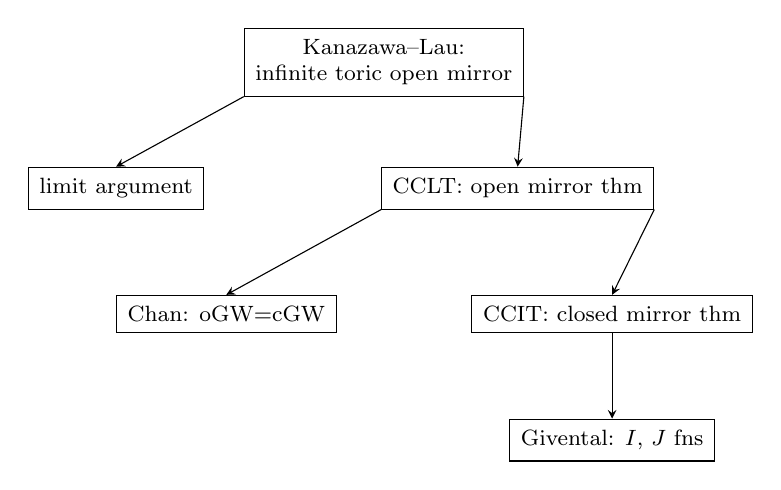
\begin{tikzpicture}[
  box/.style={draw, fill=white, inner sep=4pt, font=\footnotesize, align=center},
  arr/.style={->, >=stealth, thin}]
\node[box] (kl) at (0,0) {Kanazawa--Lau:\\infinite toric open mirror};
\node[box] (limit) at (-3.4,-1.6) {limit argument};
\node[box] (cclt) at (1.7,-1.6) {CCLT: open mirror thm};
\node[box] (chan) at (-2.0,-3.2) {Chan: oGW=cGW};
\node[box] (ccit) at (2.9,-3.2) {CCIT: closed mirror thm};
\node[box] (giv) at (2.9,-4.8) {Givental: $I$, $J$ fns};
\draw[arr] (kl.south west) -- (limit.north);
\draw[arr] (kl.south east) -- (cclt.north);
\draw[arr] (cclt.south west) -- (chan.north);
\draw[arr] (cclt.south east) -- (ccit.north);
\draw[arr] (ccit.south) -- (giv.north);
\end{tikzpicture}
\end{center}

\begin{lemma}[Givental]\label{lem:givental}
Picard--Fuchs 可计算 GWI，并且镜像于 Hodge 结构中周期的组合概念。Givental 引入了 $I$ 函数与 $J$ 函数。
\end{lemma}

\begin{remark}[闭镜像定理：{[CCIT15]}]\label{rem:closed-mirror}
我们提供一组资源，以说明理解 Gromov--Witten 不变量的时间线与背景。一侧的 $J$ 函数（Gromov--Witten 不变量）对应另一侧的 $I$ 函数（组合的）。这建立在 Givental 的工作上：镜像映射是 $1/z$ 的系数。见 [CK99, §6.3]。凯勒模与复模同构；镜像映射在凯勒大极限点的邻域与复侧的极大单值性之间。Picard--Fuchs 用于极大单值性附近的复模，[CK99] 记作 $y_k$；而 $q_k$ 用于凯勒模。GKZ 系统见 [CK99, §5.5]，Picard--Fuchs 见 §5.1.2。变复模给出 Hodge 结构的变分。§2.6.2 引入 Givental 的 $I,J$ 函数。§11.2.5 是环簇完全交的 Givental 镜像定理。第 10 章：模空间的 stack 定义。方程 (10.4) 给出微分/相交论与 GW 的关系。stack 入门的参考是 [Fan01]。[CK99, Proposition 10.3.4] 给出 $J$ 函数与 GW 势的关系。镜像定理的例子：11.2.1.3。Theorem 10.3.5：QM 微分算子当且仅当 Picard--Fuchs 算子。第 7 章给出 GW 的定义。$1/z$ 系数的陈述：[CK99, page 151]，[KL19] 中的 $z$ 即 [CK99] 中的 $y_0$。注意：据 [CK99]，Givental 镜像定理的等变性在原论文 [Giv98] 中并不完整；这正是 [CCIT15] 所讨论的。随后 [CCLT16] 加入 [Cha11] 的结果：
\[
M_X^{open}(\beta+\alpha)=M_X^{closed}(\beta+\alpha).
\]
等变性在 [CCIT15] 中讨论，因为那里是环簇设定。
\end{remark}

% ===== 原书 p.128 =====
\begin{definition}[Kuranishi 结构]\label{def:kuranishi}
$p$ 的 Kuranishi 邻域具有以下性质：
\begin{itemize}[leftmargin=2.2em,itemsep=0.25em]
\item $V_p$ 是光滑有限维\emph{流形}，可带角；
\item $V_p\times E_p\to V_p$ 称为\emph{障碍丛}（$E_p$ 是有限维实\emph{向量空间}）；
\item $\Gamma_p$ 是有限\emph{群}，光滑且有效地作用在 $V_p$ 上（无非平凡元素平凡作用），并在 $E_p$ 上线性地表示该群；
\item \emph{Kuranishi 映射} $s_p$ 是 $V_p\times E_p$ 的光滑\emph{截面}（光滑映射 $V_p\to\Gamma_p$），且是 $\Gamma_p$-等变的；
\item $\psi_p$ 是\emph{拓扑卡}，即从局部模型 $s_p^{-1}(0)/\Gamma_p$ 到 $X$ 中 $p$ 的一个邻域的同胚；
\item $V_p/\Gamma_p$ 也可称为一个 \emph{Kuranishi 邻域}（而不是指上述所有数据之集）。事实上 $V_p$ 也可称为 Kuranishi 邻域。于是有三样不同的东西都可叫邻域；
\item $o_p$ 是一个点，Kuranishi 映射把它送到零，卡把它送到 $p$。
\end{itemize}
\end{definition}
% [Tutor Note: 原文第三条括号内作「smooth map V_p → Γ_p」，与 Kuranishi 映射为 V_p × E_p 的截面不合；按定义应为 V_p → E_p。译文保留原样，登记于报告。]

\transnote{本页 Kuranishi 结构定义的第三条最易读错：原文括号里写 $V_p\to\Gamma_p$，但 Kuranishi 映射是障碍丛 $V_p\times E_p\to V_p$ 的截面，因此应理解为 $V_p\to E_p$。$\Gamma_p$ 是作用在 $V_p$ 与 $E_p$ 上的有限群，不是映射的靶。译文保留原文写法并在报告中登记。}

Gromov--Witten 不变量是具有 Kuranishi 结构的一个例子，因为该结构的定义刻画的正是这类模空间的局部图景。另见 [MTFJ19]。

[KL19] 中有取极限以到达无限环簇情形的概念，本文也如此。它建立在 CCLT 开镜像定理之上。Kanazawa--Lau 做球计数：$1/z$ 的系数就是镜像映射。

\begin{theorem}[{[KL19, Theorem 3.10]} 中的开镜像定理]\label{thm:open-mirror}
设 $Y$ 是无限型的环簇 Calabi--Yau 流形。则
\[
\sum_{\alpha}n_{\beta_l+\alpha}q^{\alpha}(\check q)=\exp(g_l(\check q)),
\]
其中 $q(\check q)$ 是镜像映射，且
\[
g_l(\check q):=\sum_d\frac{(-1)^{(D_l\cdot d)}(-(D_l\cdot d)-1)!}{\prod_{p\ne l}(D_p\cdot d)!}\check q^d.
\]
\end{theorem}

至此，[KL19] 球泡计数的证明梗概结束。

% ===== 原书 p.129 =====
\medskip\noindent\textbf{在定义中计入计算时所用的非正则 $J$}\par
此时我们使用 polyfold（感谢 Benjamin Fillippenko 的协助）。我们要考虑的 $\overline{\mathcal{M}}_\beta(J)$ 为
\begin{align*}
\overline{\mathcal{M}}_\beta(J):=\bigl\{(u,\underline{v})&:(\mathbb{D},(S^2)^k)\to Y \bigm| u(\partial\mathbb{D})\subset T_z|_{C_r},\\
&[u\#v]=\beta,\ (u,\overline{v})\in C^\infty,\ ev_{z_0}(0)=ev(z_1)(z),\ \overline{\partial}_J(u,v)=0\bigr\}\times\{p\}/\operatorname{Aut}(Y,p),
\end{align*}
它目前只是一个集合。定义集合 $\mathcal{B}_\beta$ 为去掉 $J$-全纯条件后上述对象的完备化。这与几何情形类似，区别在于维数与构型不同。整个设定具有 polyfold 结构，见 Jiayong Li 的学位论文。它以光滑映射之集为稠密子集。$\mathcal{B}_\beta$ 上的丛也应有 polyfold 结构，其定义就是使 $\overline{\partial}_J$ 逐纤维落入其中的那个正确对象。

这有 Fredholm/polyfold 设定与合适的截面。我们可以扰动；不同扰动之间有配边，故它关于扰动不变。变 $J$ 之间也有配边。特别地，若从正则 $J$ 出发，则扰动为零，于是得到它与扰动后模空间（实际上是一个流形）之间的配边。最后，我们用 W. Schmaltz 学位论文的结果：可容扰动的拉回仍是可容的，只要映射满足适当条件，而这里的映射满足。于是我们发现，不同圆盘的所有模空间都出现相同的球构型。这里用到 polyfold 中 EP groupoid 的机器。

由 [CLL12] 的结果，紧化中可能出现的同调类只有形如 $D_{ij}+\sum_i n_i\alpha_i$ 的稳定树，其中 $n_i$ 是整数，$\alpha_i$ 是球。目标是证明：固定 $D_{ij}$ 并紧化后，对任意其他 $D_{ij}$ 都得到相同的紧化。也就是说，变同调类时所有模空间同构；施加群作用，得到与 $J_0$ 相同的同构模空间，而这些模空间的存在性已由上述讨论知道。这样，无论含 $D_{ij}$ 的紧化中的计数是什么，含 $\gamma(D_{ij})$ 的紧化都涉及同构的模空间；故计数相同，可以提出一个公因子：
\[
\mathcal{M}(D+\alpha_i,J_0)\cong\mathcal{M}(\gamma(D+\alpha_i),\gamma^*J_0),
\]
其中同构由在 $Y$ 的覆盖上（取 $\Gamma_B$ 商之前）与 $\gamma$ 复合给出。注意结果全纯，因为我们用的是 $\gamma^*J_0$；但数乘是全纯映射，故 $\gamma^*J_0=J_0$，两模空间同构。

于是 GW 理论与 polyfold 理论给出的 FS 范畴，与只考虑无球圆盘所算出的 FS 范畴等价。而圆盘计数给出 theta 函数。

\transnote{$\overline{\mathcal{M}}_\beta(J)$ 的定义里符号混用：$(u,\underline{v})$ 中的 $v$ 带下划线，而 $(u,\overline{v})$ 中的 $v$ 带上横线，$ev_{z_0}(0)=ev(z_1)(z)$ 中的赋值映射也未说明靶空间。作者是在记笔记，不是给正式定义。译文照原样排出，读者不必在符号上深究，抓住「圆盘、球、边界在 $T_z$、过奇异纤维一次、再商去 $\operatorname{Aut}(Y,p)$」即可。}

% ===== 原书 p.130 =====
\subsection{证明：全忠实嵌入 $\DBCoh(H)\into H^0(\mathrm{FS}(Y,v_0))$}

在对象上，我们映射 $\mathcal{L}|_H^{\otimes i}\mapsto L_i$。若 $\phi$ 是辛纤维丛 $v_0:Y\to\C$ 绕原点的单值性，则 $\omega$ 定义的对称性保证 $\phi(\ell_i)$ 哈密顿同痕于 $\ell_{i+1}$。由于 Floer 上同调在哈密顿同痕下不变，我们可以只考虑纤维中的线性拉格朗日。当 $j\ge i+2$ 时，由此得到下图中下面一行。当 $j<i+2$ 时还要考虑 Ext 群，得到的是长正合列；也就是说，最右的水平映射不再满。

\[
\begin{tikzcd}[column sep=4.4em, row sep=3.6em]
\Hom(\mathcal{L}^{i+1},\mathcal{L}^j)
  \arrow[r,"\otimes s"] \arrow[d,"\cong"] &
\Hom(\mathcal{L}^{i},\mathcal{L}^j)
  \arrow[r] \arrow[d,"\cong"] &
H^0(\mathcal{L}^{i},\mathcal{L}^j\otimes\iota_*\mathcal{O}_H)
  \arrow[r] \arrow[d] & 0\\
CF(\ell_{i+1},\ell_j)
  \arrow[r,"\partial"] &
CF(\ell_i,\ell_j)
  \arrow[r] &
HF(L_i,L_j)
  \arrow[r] & 0
\end{tikzcd}
\]

映射 $\partial$ 是 $CF(L_i,L_j)\cong CF(\ell_{i+1},\ell_j)[-1]\oplus CF(\ell_i,\ell_j)$ 上 Floer 微分的一部分，它数 $v_0:Y\to\C$ 的、具合适拉格朗日边界条件的全纯截面。左侧前两个竖直同构来自阿贝尔簇情形。作者的结果是：图中左侧方块交换，于是最右的竖直箭头也是同构。更精确地说，在所选同构下，Floer 微分 $\partial$ 与乘 $s\in H^0(V,\mathcal{L})$ 一致，至多差一个乘性因子（即 [KL19] 中特定凯勒参数选择下的开 Gromov--Witten 不变量）。这就给出函子 $\DBCoh(H)\to\mathrm{FS}(Y,v_0)$ 的态射群之间所要的同构。

\transnote{此图的两行分别是代数和辛几何：上排是 $H$ 上相干层的 Hom 与 $H^0$，下排是 Floer 链复形与 Floer 上同调。作者已把上排的最右项写成 $0$（当 $j\ge i+2$）；$j<i+2$ 时这一项要换成 Ext 群，图变成一条长正合列。判定全忠实的关键就是左侧方块的交换性。}

% EN48 c10 | 原书 p.131（PDF 140） | 第 6 章 记号
% 骨架文件：标题行已设定，正文由译者填写。每页起首用 % ===== 原书 p.N ===== 注释标记。
\section{记号}

% ===== 原书 p.131 =====
\medskip\noindent\textbf{1.2 节}\par
\begin{itemize}[leftmargin=2.2em,itemsep=0.25em]
\item $H=\Sigma_2$：亏格 2 曲线；
\item $V=(\C^*)^2/\Gamma_B$：阿贝尔簇，$H$ 是它的超曲面；
\item $\mathcal{L}\to V$：$V$ 上次数为 $(1,1)$ 的线丛；
\item $s:V\to\mathcal{L}$：多 theta 函数（multi-theta function），即 $\mathcal{L}$ 的截面；
\item $\lambda$：线性形式，决定 $\mathcal{L}$ 的 Chern 类；
\item $\kappa$：二次形式，决定 $\mathcal{L}$ 的全纯结构。
\end{itemize}

\medskip\noindent\textbf{1.3 节}\par
\begin{itemize}[leftmargin=2.2em,itemsep=0.25em]
\item $M$：特征格，或环簇上的函数格；
\item $N$：余特征格，或环簇的单参数子群格；
\item $M_\R=M\otimes_\Z\R$，$N$ 同理；
\item $m$：$M$ 或 $M_\R$ 的元素；
\item $u$：$N$ 中的格元素。
\end{itemize}

\medskip\noindent\textbf{1.4 节}\par
\begin{itemize}[leftmargin=2.2em,itemsep=0.25em]
\item $\widetilde{\Delta}_Y$：定义 $\widetilde{Y}$ 的多面体；
\item $\Delta_Y=\widetilde{\Delta}_Y/\Gamma_B$；
\item $(\xi_1,\xi_2,\eta)\in M_\R/\Gamma_B\cong\R^3/\Gamma_B$：表示多面体上的坐标；
\item $v_0:Y\to\C$：超势；
\item $V^\vee\cong(\C^*)^2/\Gamma_B$：$v_0$ 的纤维。
\end{itemize}

\transnote{$\Gamma_B$ 是第 1 章引入的格，作用在 $(\C^*)^2$ 上；本页是记号表，只列出记号而不重复定义。阅读此处时应回头参看第 1 章的相应约定。}

\transnote{本节的小标题「1.2 节」「1.3 节」「1.4 节」指向原书正文的章节，不是本译注的章节编号。列出的是各节所用记号的汇总，条目顺序照原文，未重新分类。}

\transnote{$\Delta_Y$ 与 $\widetilde{\Delta}_Y$ 只差一个商：$\widetilde{\Delta}_Y$ 是万有覆盖上的多面体，$\Delta_Y$ 则是取 $\Gamma_B$ 商之后的多面体。两者在原文中都用 $\Delta$ 系记号，容易混淆；凡出现商的情形，本文保留下标与 tilde 的区别。}

% EN48 c11 | 原书 p.132–136（PDF 141–145） | 参考文献
% 骨架文件：标题行已设定，正文由译者填写。每页起首用 % ===== 原书 p.N ===== 注释标记。
\section*{参考文献}
\addcontentsline{toc}{section}{参考文献}

\begingroup
\small
\begin{description}[leftmargin=7.4em, labelwidth=6.8em, labelsep=0.6em,
                   font=\normalfont, itemsep=0.35em, parsep=0pt]

% ===== 原书 p.132 =====
\item[{[AAK16]}] Mohammed Abouzaid, Denis Auroux, and Ludmil Katzarkov, \emph{Lagrangian fibrations on blowups of toric varieties and mirror symmetry for hypersurfaces}, Publ. Math. Inst. Hautes \'Etudes Sci. \textbf{123} (2016), 199--282.
\item[{[Abo09]}] Mohammed Abouzaid, \emph{Morse homology, tropical geometry, and homological mirror symmetry for toric varieties}, Selecta Math. (N.S.) \textbf{15} (2009), no. 2, 189--270.
\item[{[ACGK12]}] Mohammad Akhtar, Tom Coates, Sergey Galkin, and Alexander M. Kasprzyk, \emph{Minkowski polynomials and mutations}, SIGMA Symmetry Integrability Geom. Methods Appl. \textbf{8} (2012), Paper 094, 17.
\item[{[APS]}] Nicolas Addington, Alexander Polishchuk, and Ed Segal, \emph{Summer graduate school, derived categories}, \url{https://www.msri.org/summer_schools/821}.
\item[{[AS]}] Mohammed Abouzaid and Paul Seidel, \emph{Lefschetz fibration methods in wrapped Floer cohomology}, in preparation.
\item[{[AS10]}] Mohammed Abouzaid and Ivan Smith, \emph{Homological mirror symmetry for the 4-torus}, Duke Math. J. \textbf{152} (2010), no. 3, 373--440.
\item[{[Aur07]}] Denis Auroux, \emph{Mirror symmetry and T-duality in the complement of an anti-canonical divisor}, J. G\"okova Geom. Topol. GGT \textbf{1} (2007), 51--91.
\item[{[Aur14]}] ---, \emph{A beginner's introduction to Fukaya categories}, Contact and symplectic topology, Bolyai Soc. Math. Stud., vol. 26, J\'anos Bolyai Math. Soc., Budapest, 2014, pp. 85--136.
\item[{[BD16]}] Marco Bonatto and Dikran Dikranjan, \emph{Generalize Heisenberg Groups and Self-Duality}, arXiv e-prints (2016), arXiv:1611.02685.
\item[{[Bej18]}] Dori Bejleri, \emph{The SYZ conjecture via homological mirror symmetry}, Superschool on derived categories and D-branes, Springer Proc. Math. Stat., vol. 240, Springer, Cham, 2018, pp. 163--182.

% ===== 原书 p.133 =====
\item[{[BFW17]}] Nate Bottman, Joel Fish, and Katrin Wehrheim, \emph{Polyfold theory towards the fukaya category, june 12-16, 2017 at uc berkeley}, \url{http://www.polyfolds.org/index.php?title=RTG_workshop_program}, 2017.
\item[{[BJ07]}] B.H. Bransden and Charles Joachain, \emph{Quantum mechanics (second edition)}, Prentice Hall-Pearson, Harlow, England, January 2007.
\item[{[BL04]}] Christina Birkenhake and Herbert Lange, \emph{Complex abelian varieties}, second ed., Grundlehren der Mathematischen Wissenschaften [Fundamental Principles of Mathematical Sciences], vol. 302, Springer-Verlag, Berlin, 2004.
\item[{[Can]}] Catherine Cannizzo, \emph{Homological mirror symmetry for the genus 2 curve in an abelian variety and its generalized Strominger-Yau-Zaslow mirror}, Ph.D. thesis, University of California, Berkeley, in preparation: \url{https://math.berkeley.edu/~cannizzo/Cannizzo_draft_Oct_31}.
\item[{[CCIT15]}] Tom Coates, Alessio Corti, Hiroshi Iritani, and Hsian-Hua Tseng, \emph{A mirror theorem for toric stacks}, Compos. Math. \textbf{151} (2015), no. 10, 1878--1912.
\item[{[CCLT16]}] Kwokwai Chan, Cheol-Hyun Cho, Siu-Cheong Lau, and Hsian-Hua Tseng, \emph{Gross fibrations, SYZ mirror symmetry, and open Gromov-Witten invariants for toric Calabi-Yau orbifolds}, J. Differential Geom. \textbf{103} (2016), no. 2, 207--288.
\item[{[CdlOGP91]}] Philip Candelas, Xenia C. de la Ossa, Paul S. Green, and Linda Parkes, \emph{A pair of Calabi-Yau manifolds as an exactly soluble superconformal theory}, Nuclear Phys. B \textbf{359} (1991), no. 1, 21--74.
\item[{[Cha11]}] Kwokwai Chan, \emph{A formula equating open and closed Gromov-Witten invariants and its applications to mirror symmetry}, Pacific J. Math. \textbf{254} (2011), no. 2, 275--293.
\item[{[CK99]}] David A. Cox and Sheldon Katz, \emph{Mirror symmetry and algebraic geometry}, Mathematical Surveys and Monographs, vol. 68, American Mathematical Society, Providence, RI, 1999.
\item[{[CLL12]}] Kwokwai Chan, Siu-Cheong Lau, and Naichung Conan Leung, \emph{SYZ mirror symmetry for toric Calabi-Yau manifolds}, J. Differential Geom. \textbf{90} (2012), no. 2, 177--250.
\item[{[CLS11]}] David A. Cox, John B. Little, and Henry K. Schenck, \emph{Toric varieties}, Graduate Studies in Mathematics, vol. 124, American Mathematical Society, Providence, RI, 2011.

% ===== 原书 p.134 =====
\item[{[CO06]}] Cheol-Hyun Cho and Yong-Geun Oh, \emph{Floer cohomology and disc instantons of Lagrangian torus fibers in Fano toric manifolds}, Asian J. Math. \textbf{10} (2006), no. 4, 773--814.
\item[{[Fan01]}] Barbara Fantechi, \emph{Stacks for everybody}, European Congress of Mathematics, Vol. I (Barcelona, 2000), Progr. Math., vol. 201, Birkh\"auser, Basel, 2001, pp. 349--359.
\item[{[FOOO09a]}] Kenji Fukaya, Yong-Geun Oh, Hiroshi Ohta, and Kaoru Ono, \emph{Lagrangian intersection Floer theory: anomaly and obstruction. Part I}, AMS/IP Studies in Advanced Mathematics, vol. 46, American Mathematical Society, Providence, RI; International Press, Somerville, MA, 2009.
\item[{[FOOO09b]}] ---, \emph{Lagrangian intersection Floer theory: anomaly and obstruction. Part II}, AMS/IP Studies in Advanced Mathematics, vol. 46, American Mathematical Society, Providence, RI; International Press, Somerville, MA, 2009.
\item[{[For91]}] Otto Forster, \emph{Lectures on Riemann surfaces}, Graduate Texts in Mathematics, vol. 81, Springer-Verlag, New York, 1991, Translated from the 1977 German original by Bruce Gilligan, Reprint of the 1981 English translation.
\item[{[Fra10]}] J Francis, \emph{Math 465, spring 2010: Topology of manifolds}, \url{http://math.northwestern.edu/~jnkf/classes/mflds/}, 2010.
\item[{[Fuk02]}] Kenji Fukaya, \emph{Mirror symmetry of abelian varieties and multi-theta functions}, J. Algebraic Geom. \textbf{11} (2002), no. 3, 393--512.
\item[{[Ful93]}] William Fulton, \emph{Introduction to toric varieties}, Annals of Mathematics Studies, vol. 131, Princeton University Press, Princeton, NJ, 1993, The William H. Roever Lectures in Geometry.
\item[{[Gan16a]}] Sheel Ganatra, \emph{Automatically generating Fukaya categories and computing quantum cohomology}, arXiv preprint arXiv:1605.07702 (2016).
\item[{[Gan16b]}] ---, \emph{Math 257b: Topics in symplectic geometry -- aspects of fukaya categories}, \url{https://dornsife.usc.edu/sheel-ganatra/math-257b/}, 2016.
\item[{[GH94]}] Phillip Griffiths and Joseph Harris, \emph{Principles of algebraic geometry}, Wiley Classics Library, John Wiley \& Sons, Inc., New York, 1994, Reprint of the 1978 original.
\item[{[Giv98]}] Alexander Givental, \emph{A mirror theorem for toric complete intersections}, Topological field theory, primitive forms and related topics (Kyoto, 1996), Progr. Math., vol. 160, Birkh\"auser Boston, Boston, MA, 1998, pp. 141--175.

% ===== 原书 p.135 =====
\item[{[GP90]}] B. R. Greene and M. R. Plesser, \emph{Duality in Calabi-Yau moduli space}, Nuclear Phys. B \textbf{338} (1990), no. 1, 15--37.
\item[{[Huy05]}] Daniel Huybrechts, \emph{Complex geometry}, Universitext, Springer-Verlag, Berlin, 2005, An introduction.
\item[{[KL19]}] Atsushi Kanazawa and Siu-Cheong Lau, \emph{Local Calabi-Yau manifolds of type $\widetilde{A}$ via SYZ mirror symmetry}, J. Geom. Phys. \textbf{139} (2019), 103--138.
\item[{[Kon95]}] Maxim Kontsevich, \emph{Homological algebra of mirror symmetry}, Proceedings of the International Congress of Mathematicians, Vol. 1, 2 (Z\"urich, 1994), Birkh\"auser, Basel, 1995, pp. 120--139.
\item[{[KS01]}] Maxim Kontsevich and Yan Soibelman, \emph{Homological mirror symmetry and torus fibrations}, Symplectic geometry and mirror symmetry (Seoul, 2000), World Sci. Publ., River Edge, NJ, 2001, pp. 203--263.
\item[{[Laz00]}] L. Lazzarini, \emph{Existence of a somewhere injective pseudo-holomorphic disc}, Geom. Funct. Anal. \textbf{10} (2000), no. 4, 829--862.
\item[{[Laz11]}] Laurent Lazzarini, \emph{Relative frames on J-holomorphic curves}, J. Fixed Point Theory Appl. \textbf{9} (2011), no. 2, 213--256.
\item[{[Mil65]}] John Milnor, \emph{Lectures on the h-cobordism theorem}, Notes by L. Siebenmann and J. Sondow, Princeton University Press, Princeton, N.J., 1965.
\item[{[MS12]}] Dusa McDuff and Dietmar Salamon, \emph{J-holomorphic curves and symplectic topology}, second ed., American Mathematical Society Colloquium Publications, vol. 52, American Mathematical Society, Providence, RI, 2012.
\item[{[MS17]}] ---, \emph{Introduction to symplectic topology}, third ed., Oxford Graduate Texts in Mathematics, Oxford University Press, Oxford, 2017.
\item[{[MTFJ19]}] Dusa McDuff, Mohammad Tehrani, Kenji Fukaya, and Dominic Joyce, \emph{Virtual fundamental cycles in symplectic topology}, American Mathematical Society, 2019.
\item[{[Oh93]}] Yong-Geun Oh, \emph{Floer cohomology of Lagrangian intersections and pseudo-holomorphic disks. I}, Comm. Pure Appl. Math. \textbf{46} (1993), no. 7, 949--993.
\item[{[Pol03]}] Alexander Polishchuk, \emph{Abelian varieties, theta functions and the Fourier transform}, Cambridge Tracts in Mathematics, vol. 153, Cambridge University Press, Cambridge, 2003.
\item[{[PZ98]}] Alexander Polishchuk and Eric Zaslow, \emph{Categorical mirror symmetry: The Elliptic curve}, Adv. Theor. Math. Phys. \textbf{2} (1998), 443--470.

% ===== 原书 p.136 =====
\item[{[Seg]}] Graeme Segal, \emph{July-august 1999 itp workshop on geometry and physics: Topological field theory (`stanford notes')}, \url{http://web.math.ucsb.edu/~drm/conferences/ITP99/segal/}.
\item[{[Sei00]}] Paul Seidel, \emph{Graded Lagrangian submanifolds}, Bull. Soc. Math. France \textbf{128} (2000), no. 1, 103--149.
\item[{[Sei08]}] ---, \emph{Fukaya categories and Picard-Lefschetz theory}, Zurich Lectures in Advanced Mathematics, European Mathematical Society (EMS), Z\"urich, 2008.
\item[{[Sei11]}] ---, \emph{Homological mirror symmetry for the genus two curve}, J. Algebraic Geom. \textbf{20} (2011), no. 4, 727--769.
\item[{[SYZ96]}] Andrew Strominger, Shing-Tung Yau, and Eric Zaslow, \emph{Mirror symmetry is T-duality}, Nuclear Phys. B \textbf{479} (1996), no. 1-2, 243--259.
\item[{[Weh13]}] Katrin Wehrheim, \emph{Berkeley math 278: Analysis of pseudoholomorphic curves}, \url{https://piazza.com/berkeley/fall2013/berkeleymath278/resources}, 2013.
\item[{[Weh14]}] ---, \emph{Regularization of moduli spaces of pseudoholomorphic curves}, \url{https://math.berkeley.edu/~katrin/teach/regularization/lectures.shtml}, 2014.

\end{description}
\endgroup

\transnote{按工程约定，参考文献条目保留原文，不译成中文；方括号内的是原书条目标签，顺序与原文一致。同一作者的多条文献，原书用长破折号代替作者名，这里排作「———,」。期刊名与书名保持原书写法，卷号用粗体。}


\end{document}
